\documentclass[11pt]{report}
\usepackage{projectreport}

\newcommand{\name}{John W. Holden}
\newcommand{\course}{Doctor of Philosophy}
\newcommand{\projecttitle}{Mathematical and Computational Modelling of Infectious Tree Diseases}
\newcommand{\submissiondate}{September 2020}
\newcommand{\submissionyear}{2020}

\setcounter{tocdepth}{4}
\setcounter{secnumdepth}{4}
\begin{document}

\maketitle

% 0) abstract, intellectual property and acknowledgements
\chapter*{Intellectual Property}
\addcontentsline{toc}{chapter}{Intellectual Property}
The candidate confirms that the work submitted is his/her own and that appropriate credit has been given where reference has been made to the work of others.

This copy has been supplied on the understanding that it is copyright material and that no quotation from the thesis may be published without proper acknowledgement.

© \submissionyear\ The University of Leeds, \name

\vspace{2cm}
Signed 
\makebox[4cm][c]{\raisebox{-2ex}{\includegraphics[width=3cm, height=1cm]{example-image}}} % replace with your signature

\chapter*{Acknowledgements}
\addcontentsline{toc}{chapter}{Acknowledgements}
This research has been carried out by a team which has included (name the individuals). My own contributions, fully and explicitly indicated in the thesis, have been......(please specify)” The other members of the group and their contributions have been as follows: (please specify).

\chapter*{Abstract}
\addcontentsline{toc}{chapter}{Abstract}

Presently, tree populations worldwide face unprecedented threats from invasive pests and pathogens endangering ecological function, timber production and human wellbeing. 
From first principles, this thesis incrementally extends a simple percolation model of forest-based epidemics into a more involved stochastic dispersal framework combined with host data. 
% The research aims to construct robust epidemic models of tree disease over the landscape of Great Britain and afterwards optimise a novel epidemic control strategy.
The approach developed here couples two spatially-explicit epidemic models at different scales. 
First, a non-local stochastic model of pathogen dispersal between trees is constructed. 
Then, the small-scale epidemic model is projected onto a large-scale distribution of host abundance, resulting in an $R_0$-map across Great Britain. 
Subsequently, a clustering algorithm is employed to identify high-risk regions in the $R_0$-map. 
Initial results indicate a global epidemic phase transition across the distribution, conditional on an infectivity parameter.
The approach to `spatially scale' an epidemic model over the entire landscape is computationally efficient, flexible and adaptable to many pests and pathogens. 
Numerous studies have sought to understand and optimise epidemic control in botanical populations. 
The mainstream control paradigm generally seeks to optimise an `eradication radius' about infected symptomatic trees over a relatively small spatial scale. However, large-scale epidemic control based solely on the spatial distribution of hosts has yet to be explored in depth. 
As such, this thesis will also examine how host heterogeneity, combined with targeted epidemic control, can give rise to natural `pinch-points' that may slow the epidemic spread between regions. 
Ultimately, this investigation intends to help policymakers reach informed decisions about where to focus control in the landscape of Great Britain.

% Ultimately, this investigation intends to help policymakers reach informed decisions about \textit{where} to focus control in the landscape.

\newcommand{\RNum}[1]{\uppercase\expandafter{\romannumeral #1\relax}}
. 

\tableofcontents 
\listoffigures
\listoftables
\gls{alb} \gls{acb} \gls{cca} \gls{com} \gls{slm}  \gls{adb} \gls{opm} \gls{ldd}
\printglossary[title={Abbreviations},type=acronym,style=long]
\newpage
\setcounter{page}{0}
\pagenumbering{arabic}

% Uncomment to see a chapter:
% 1)  A introduction to the problem of tree disease
\chapter{Introduction}

Currently, pests and pathogens threaten the survival of numerous tree species around the globe. 
An upsurge in the trade and transport of non-native plants and the widespread adoption of monoculture plantations have drastically increased the risk of large-scale outbreaks in native tree populations.
Moreover, following the effects of climate change and increased temperatures, the threats posed by invasive non-indigenous pathogens are only set to increase. Accordingly, efforts to understand the precise mechanisms that underpin epidemics in tree populations are essential for human wellbeing and ecosystem stability.

When an epidemic takes hold, numerous challenges complicate an effective on-the-ground response. In addition, epidemic drivers are multifaceted, hard to quantify, and often unknown. 
Consequently, epidemic models are significantly challenging to parameterise. 
Further still, communicating research insight to policymakers and stakeholders poses a significant challenge for modellers even with accurate parameterisation.

Despite the complex challenges that threaten tree health, scientists, policymakers, and stakeholders can cooperate to prevent the spread of emergent infectious tree diseases within a country.
Notably, the output from mathematical models can help advise practical management strategies to control epidemics through rural and urban tree populations.
Accurate epidemic models can also help forest and woodland managers structure plantations to minimise epidemic impact. 
Aiding forest managers with mathematical models has become particularly vital given the UK government's recent measures to sequester carbon from the atmosphere with land-use change and afforestation, thereby increasing tree coverage throughout Great Britain.

This Chapter introduces the reasons, challenges, and value in modelling tree disease epidemics.
First, the overarching rationale behind researching tree disease models is highlighted, followed closely by reviewing the most pressing epidemic drivers.
Second, the challenge of implementing epidemic control is summarised, along with the principal socioeconomic relationships between modellers, policymakers and stakeholders. Finally, the Chapter concludes by outlining the topics covered in this thesis.


\section{Invasive tree diseases}

The modern world relies heavily on imports and exports characterised by global trade networks. 
Unfortunately, the trade and transport of foreign plant material can introduce invasive pests and pathogens into non-native landscapes. 
As such, crops, flowering plants and tree populations that lack evolutionary adaptations 
to these invasive (pathogenic) species face unprecedented perils \cite{doi:10.1002/9781444329988.ch8}.
Epidemics through botanical populations can be devastating.
Classic historical examples include Irish potato blight, Dutch elm disease (\acrshort{ded}) \cite{doi:10.1111/j.1365-3059.2010.02391.x} 
and North American chestnut blight \cite{doi:10.1002/9780470535486.ch7}.
Two high-profile epidemics currently underway in the UK include ash dieback (\acrshort{adb}) affecting European ash \textit{Fraxinus excelsior} (\acrshort{fe})
\cite{ash-dieback-costs}, and \textit{Phytophthora ramorum} (\acrshort{pr}), a prevalent disease affecting over 150 plant species, including oak, 
larch, and sweet chestnut \cite{p.ramourum}.

Given the fundamental significance of tree populations in terrestrial ecosystems, ensuring tree health forms a critical challenge for society to address.
In particular, policymakers can lead control initiatives to help impede the spread of disease \cite{Gilligan-disease-management}.
However, implementing an uninformed and ineffective management strategy is costly and does little to stop the spread.
Accordingly, research into optimal disease management underpins the central issue of botanical epidemiology, 
where research should ideally seek to minimise both epidemic and economic impact \cite{ash-dieback-costs, freer2017tree, boyd2013consequence, tyrvainen2005benefits}. 
Frequently, control strategies include reducing tree densities \cite{pietzsch2021effect, resiliency-density-reductions} and planting genetically diverse host distributions \cite{doi:10.1094/PD-89-0969, genetic-heterogeneity, huang1980importance}.

\subsection{Epidemic drivers}

The terms `pest' and `pathogen' describe a broad spectrum of taxonomically diverse organisms. Pests denote any organism that harms humans or human interests, such as crops or livestock \cite{buckle2015rodent, oerke2006crop, de1964biological}. Overwhelmingly, insects constitute the main
pest threats to tree species \cite{metcalf1994introduction}. In Great Britain (\acrshort{gb}), the Asian longhorn beetle (\acrshort{alb}) \cite{haack2010managing}, and oak processionary moth (\acrshort{opm}) \cite{tomlinson2015managing} are two such pests that currently threaten tree health.
In contrast, the term `pathogen' describes any organism that induces disease. In the context of tree populations, diseases include fungi, bacteria, viruses, and oomycetes \cite{balloux2017q, Boyd1235773}. Presently, the oomycete \textit{P. ramorum} \cite{brasier2005phytophthora}, and ADB
caused by the fungus \textit{H. fraxineus} (\acrshort{hf}) \cite{ash-dieback-costs, mitchell2014ash} are two pathogens that threaten tree-health in GB.

Tree pathogens have evolved diverse reproductive modes and epidemiologies,  characterising a distinctive challenge when controlling tree-based pathogens. Two contrasting examples include chestnut blight caused by the bark pathogen fungus \textit{ Cryphonectria parasitica} and the xylem inhibiting bacterium \textit{Xylella fastidiosa}\footnote{Several diseases are symptomatic expressions of \textit{X. fastidiosa}, including phoney peach disease, quick olive decline, coffee leaf scorch, and most notably, Pierce's disease affecting Grapes and citrus variegated chlorosis \cite{hopkins2002xylella}.}. 
Chestnut blight devastated American chestnut populations in the 1930s \cite{doi:10.1002/9780470535486.ch7}, and more recently, infections have been spreading through European chestnuts, albeit to a lesser extent \cite{heiniger1994biological}.
The principal infection mechanism of \textit{ C. parasitica} occurs through windborne spore dispersal into wounds or openings in bark. 
In contrast, transmission of the bacterium \textit{X. fastidiosa} is thought to occur exclusively through sap-sucking insect vectors, e.g leafhoppers of the genus \textit{Homoptera} \cite{redak2004biology}. 
One remarkable facet of \textit{X. fastidiosa} is its ability to infect numerous tree species. Current estimates indicate the host range of \textit{X. fastidiosa} is upwards of 611 different plant species \cite{european2022update}, whereas \textit{C. parasitica} predominantly infects chestnut species and occasionally nearby oak \cite{rigling2018cryphonectria}. 

The trade and transport of non-native plant material are widely recognised to risk introducing invasive pests and pathogens into native landscapes \cite{POTTER201761, lovett2016nonnative, roy2014increasing}.
Ensuing epidemics can overwhelm botanical species lacking genetic resistance to the invasive species \cite{desprez2016evolutionary}, better understood from an evolutionary perspective: in a natural environment unaltered by human transportation, tree species co-evolve with invasive pathogens in a `gene-for-gene' arms race \cite{Thrall1735, dangl2001plant, flor1971current}.
The spread of Dutch elm disease in the UK \cite{doi:10.1111/j.1365-3059.2010.02391.x} and chestnut blight
in North America \cite{doi:10.1002/9780470535486.ch7} are two classic examples that shook the world.

Trade regulations on plant imports are essential to prevent the initial introduction of invasive pathogens \cite{rodoni2009role}, exemplified by the Dutch elm disease epidemic in the UK. 
Had more stringent regulations been active in the 1960s, elm timber infected with scolytid bark beetles (carrying the fungus \textit{Ophiostoma novo‐ulmi}) might have prevented the devastating outbreak \cite{doi:10.1111/j.1365-3059.2010.02391.x}. 
Ordinarily, these preventative measures take the form of customs checks on imported/exported timber, crops or horticultural goods. 
Recently, the European Commission enacted plant passports to regulate how growers and traders can transport plant material between countries \cite{wulfert2010implementation}.

If checks and policy implementations fail, a pathogen might be introduced into the landscape and spread through natural
dispersal pathways. Alternatively, a pathogen might be transported into foreign ecosystems through atmospheric 
long distance dispersal (\acrshort{ldd}) \cite{brown2002aerial}. In any case, biological control becomes necessary. 
The biological control of plant-based disease
can be achieved in numerous ways. Commonly, this involves chemical agents such as pesticides, predatory insects or planting
genetically resistant cultivars \cite{pal2006biological, baker1974biological}. 

In this work, we aim to construct epidemic models and investigate eradication strategies
entailing the removal of trees through sanitation felling. 
In this pursuit, three questions are vital to consider: 
(1) How do we effectively identify an infected tree? 
(2) How can we optimise tree felling to slow the spread of disease given limited resources/budgets?
(3) What is the risk that a large-scale epidemic will result from the initial observations of diseased trees?

\section{Modelling and policy}
\label{sec:modelling-and-policy}

The benefit of controlling an epidemic should outweigh the costs of letting an outbreak spread unchecked. 
Plant disease modellers can help infer well-designed control policies that maximally reduce epidemic impact and minimise the expenditure
of resources\textemdash both natural and economic. However, achieving this in practice is problematic due to various unknowns \cite{13-challenges}, and history gives examples of insufficient control policies that fail to halt pathogen spread. 
Prominent examples include the mismanagement of Dutch elm disease in the late 1960s and early 1970s \cite{dutch-elm-mismanage}, and more recently citrus canker in Florida \cite{schubert2001meeting}.

We can attempt to understand what dictates the optimal control of tree disease epidemics with mathematical models. 
Control strategies have been explored on both smaller \cite{risk-potential-control} and larger landscapes \cite{large-scale-control2}. 
On all spatial scales, consensus agrees that the effort and resources required to control an epidemic depend significantly on the scale of the epidemic at hand. That is, \textit{'aggressive pathogens should be met with aggressive control'}, as confirmed by modelling studies \cite{control-scale-matching, WEBIDEMICS}. 
In any scenario, an on-the-ground response must be carried out swiftly. Otherwise, the likelihood of successful management decreases rapidly, and the cost of inaction  soars.

The management of citrus huanglongbing (HLB) disease epidemics in California provides an insightful example of how mathematical models can be used to determine practical regulations to suppress the spread of disease, see \cite{mcroberts2019using}. Another relevant example comes from sudden oak death (SOD) management in California.
In particular, modelling SOD epidemics in California indicates that culling infested trees on the disease front's leading-edge is more effective \cite{large-scale-control}\textemdash see section \ref{sec:lr-large-scale-spread} for a more in-depth discussion of the manuscript. Subsequently, this finding helped inform targeting control in the work plan put forward by the California Oak Mortality Task Force\footnote{The reader can find further information on the California Oak Mortaility Task Force here \cite{palmieri2006california}, and download the work plan by visiting https://www.suddenoakdeath.org/} for 2017-2022.

Conventional eradication strategies involve detecting symptomatic trees and culling neighbours within a radius, e.g. \cite{WEBIDEMICS}.
A naive strategy that indiscriminately culls hosts can be fine-tuned and optimised to maximally reduce the epidemic impact. 
For example, one strategy prioritises targets by ranking hosts according to expected number of secondary infections \cite{risk-potential-control}.
Over larger spatial scales, models of sudden oak death (\acrshort{sod}) in California indicate that epidemics are most effectively controlled by targeting infected trees either at or ahead of the infectious wave-front \cite{large-scale-control}.
Nevertheless, various factors complicate eradication regardless of the spatial scale, such as the cryptic nature of tree diseases and fluctuating government budgets \cite{control-theory, control-theory-application}.

Enhanced surveillance and monitoring strategies also seek to optimise resource allocations. 
Surveillance aims to detect infected individuals and disease incidence, generally requiring the collection and analysis of epidemic data \cite{surveillance-review}.
Ultimately, surveillance and monitoring comprise the last line of defence after preemptive border checks and inspections have failed to prevent the introduction of disease. 
Statistical approaches have been adopted to optimise the number of samples/surveys required to infer disease incidence accurately \cite{yamamura2016sampling}.
Moreover, optimal surveillance strategies have been examined with logistic \cite{parnell2012estimating} and mechanistic \cite{WEBIDEMICS} epidemic models\textemdash the next Chapter offers a more in-depth review of these modelling paradigms. 

Several governmental bodies have a stake in the surveillance and monitoring of tree health in the UK, often collaborating their efforts. For example, the National Forest Inventory (NFI) conduct general surveys to determine tree distributions and woodland composition\textemdash discussed more in section \ref{ch2:hostdata}. Subsequently, output from NFI surveys is utilised by  'Forestry Research' (FR), the research agency of the Forestry Commission (FC). In addition, the FC plays a vital role in surveying landscapes for infectious tree diseases in the UK \cite{ryle1969forest, james1990history}, often responding to high-risk invasions in a more targeted capacity. Historically, the UK government has tasked the FC to undertake comprehensive large-scale surveys in response to Dutch elm disease in the 1960s-1970s \cite{potter2011learning} and ash dieback in 2012 \cite{tomlinson2016discovery}. 
However, citizen science-based approaches have become increasingly utilised to monitor tree health \cite{brown2020role}, exemplified by the monitoring tool 'TreeAlert', a website owned by FR designed to collect information about tree health in woodlands and forests through user reports.

Even supposing an accurate and well-informed control strategy,
a response on the ground only ensues when stakeholders implement control initiatives \cite{reed2018theory}. Here, the term `stakeholder' is extensive, reflecting any interested individual, collective, or organisation with a stake in tree health that has the potential to influence or affect a policy direction or control decision \cite{brugha2000stakeholder}. The UK's stakeholder landscape for tree health is equally broad, encompassing diverse governmental and private sector organisations and individuals. A conceptual framework for stakeholder categorisation was put forward by \cite{dandy2017has}, alongside a case study of who had a stake in ash dieback in the UK. In their analysis, \cite{dandy2017has} listed various affected stakeholders:
\begin{itemize}
    \item \textbf{governmental}: DEFRA, FERA, FC, FR and various local authorities
    \item \textbf{civil society/third sector}: National Trust, Wildlife Trust, Woodland Trust
    \item \textbf{private sector}: private land managers, outdoor recreationists, forest owners, citizen scientists, and the general public
\end{itemize}


%Todo:tidy up below paragraph in relation to updated diagram
Figure \ref{fig:modelling-and-policies} presents a simplified view of the interactions which dictate research output, public awareness, 
policymaking and the eventual epidemic control in the UK\footnote{
In part, Figure \ref{fig:modelling-and-policies} was informed by interviewing civil servants, researchers and policymakers at DEFRA and FERA as part of this thesis.}. Scientists in several disciplines,
from molecular biology to mathematics, receive funding from and collaborate with policymakers and other research bodies, e.g. the Department for Environment Food \& Rural Affairs (\acrshort{defra}). Policymaker-led control initiatives, resource allocation and recommendations then help to direct on-the-ground stakeholder
responses. However, it is worthwhile to remark that stakeholder participation can be either voluntary or compelled by law in the UK. Typically, if the pest or pathogen possesses a significant risk, plant health authorities (e.g. FC and DEFRA) may serve a statutory plant Health notice (SPHN) to the landowner, thus mandating action.

\begin{figure}
    \centering
    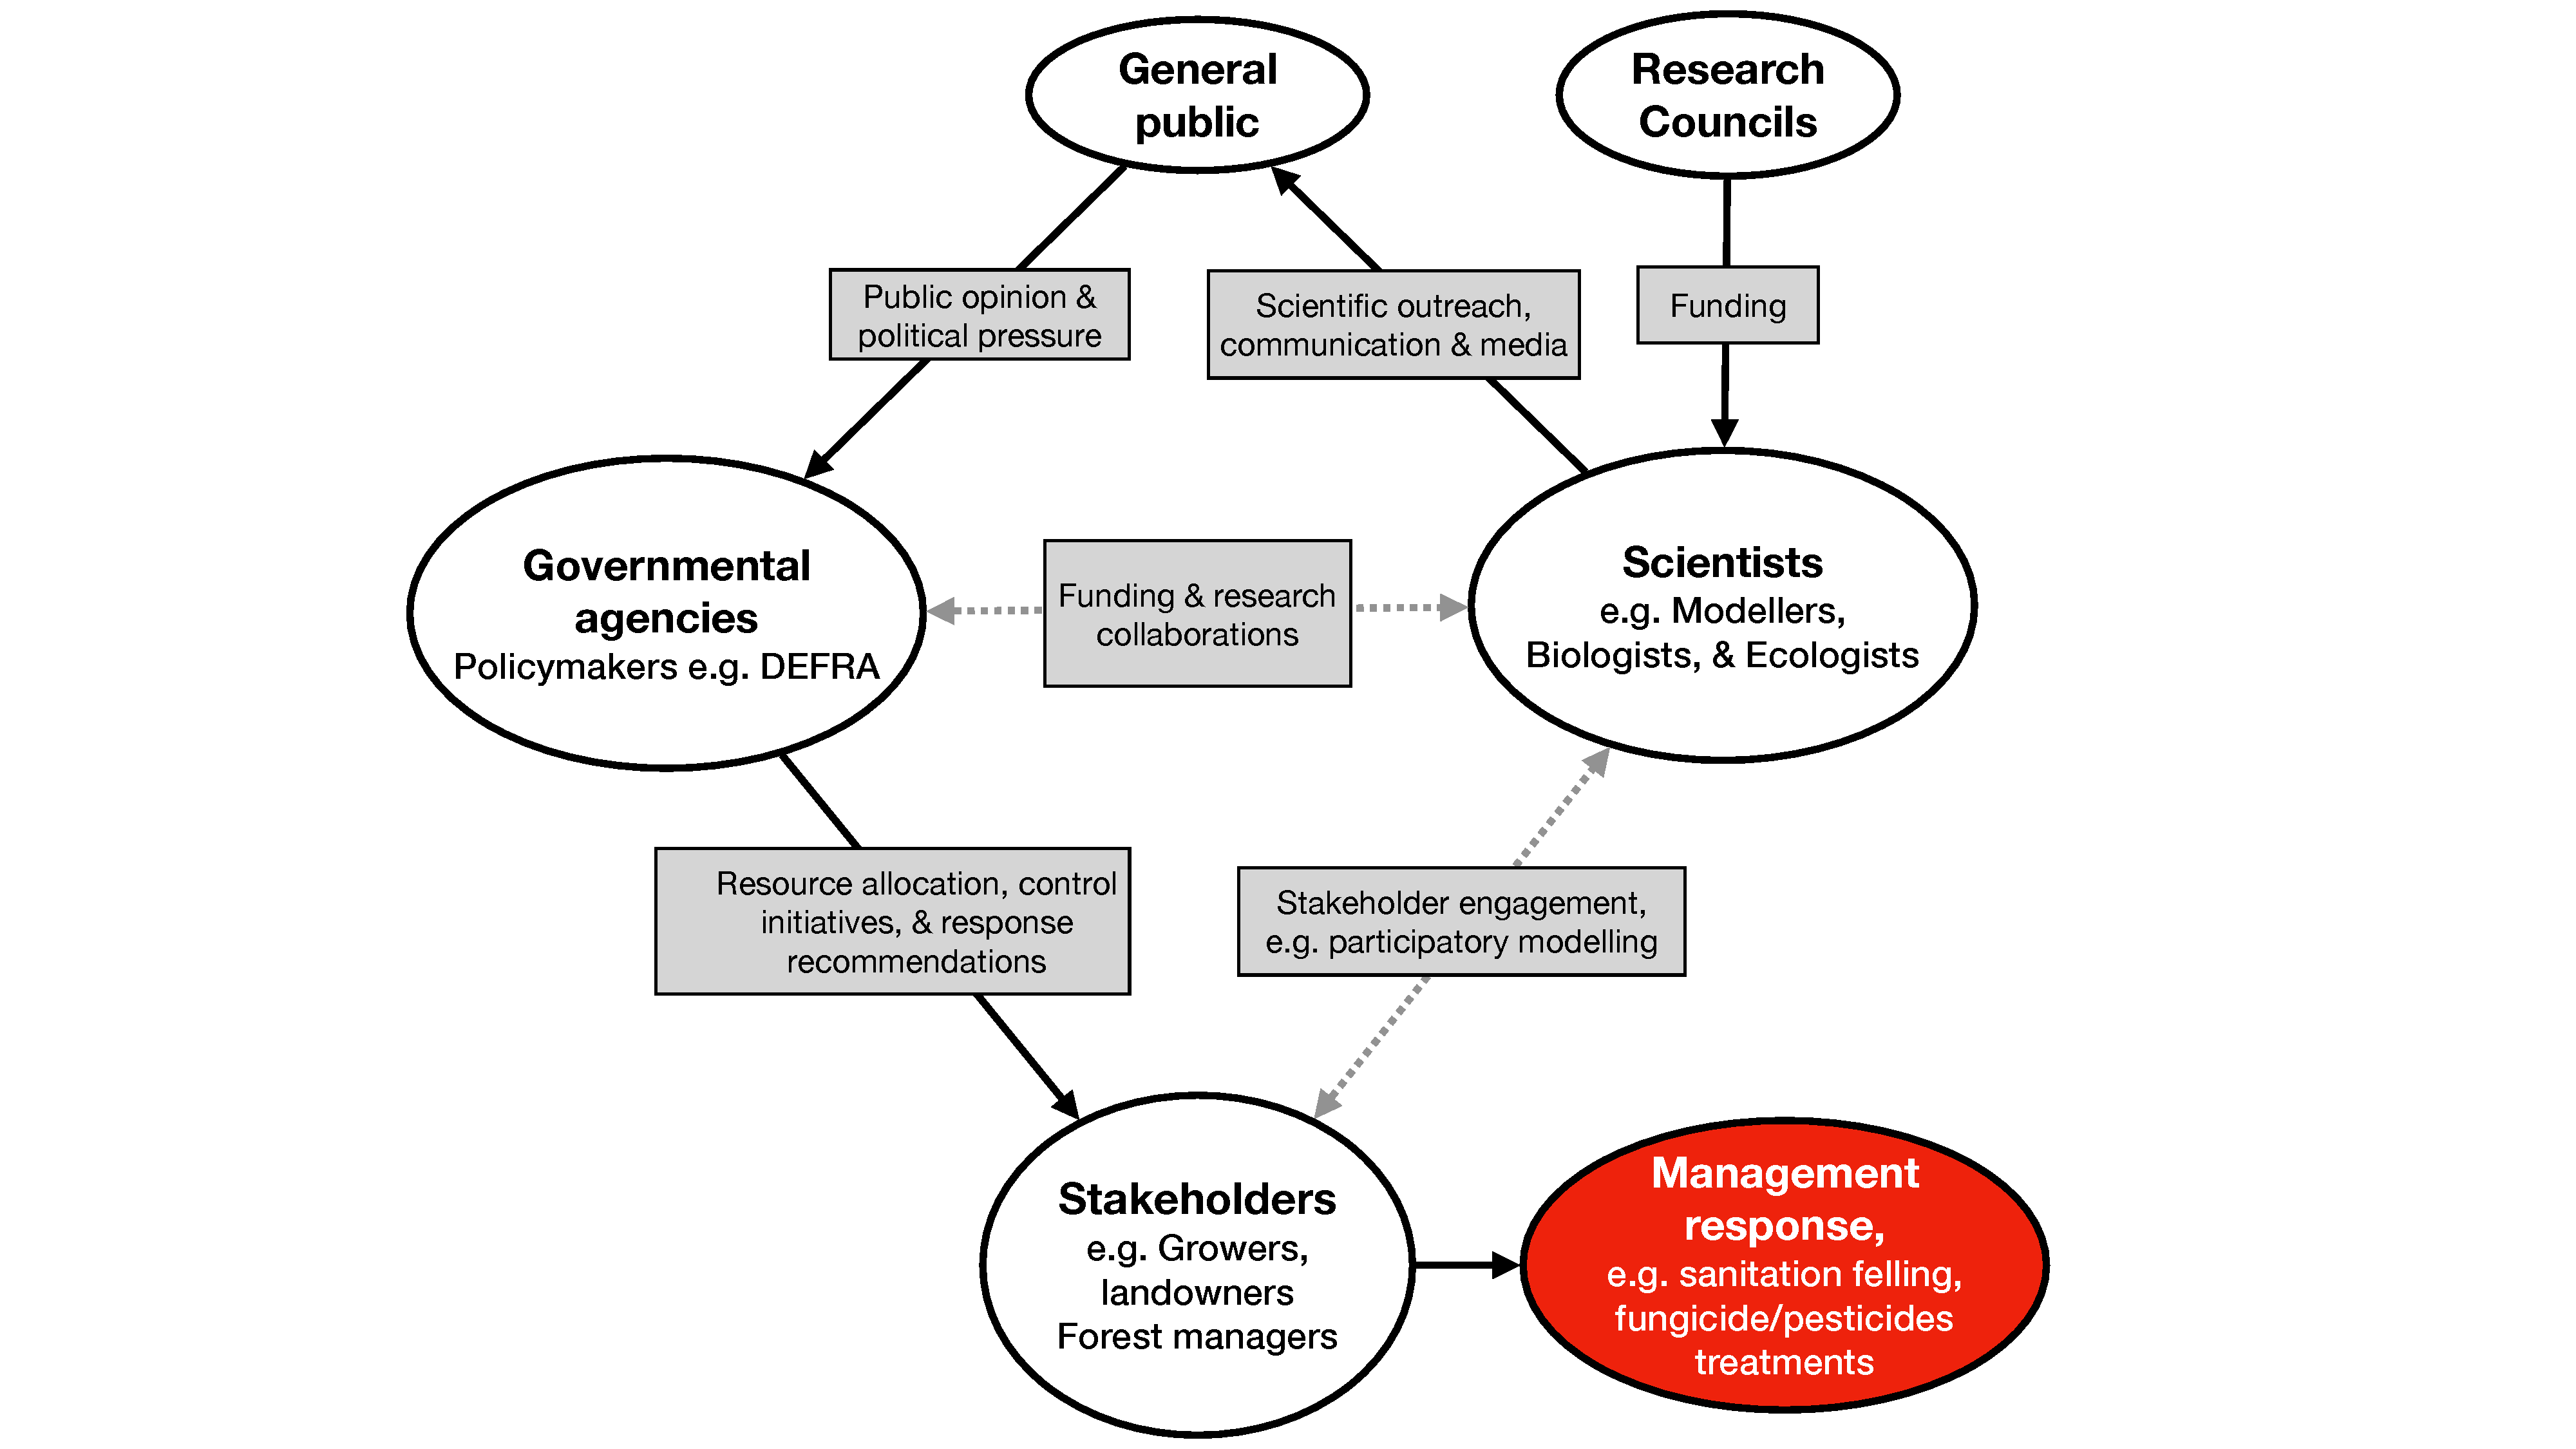
\includegraphics[scale=0.35]{chapter1/figures/modelling-and-policy.pdf}
    \caption{A simplified model representing the major socioeconomic interactions between the general public, scientists, policymakers and stakeholders in the UK. Scientists receive funding from and collaborate with Governmental bodies/policymakers. Policymakers make decisions and allocate resources to lead control initiatives to protect tree health. Affected stakeholders in the UK can choose to join voluntary control initiatives or be legally obliged to take action if served a statutory plant health notice. }
    \label{fig:modelling-and-policies}
\end{figure}

Alternatively, scientists can engage stakeholders directly (discussed more below) or influence public opinion through outreach and
scientific communication. In turn, the public can influence the decisions of policymakers by
mounting sufficient political pressure \cite{fuller2016public}.
Unfortunately, several obstacles inhibit a well-informed, timely and effective response. 
In particular, poor accessibility to scientific research is widely-known to inhibit policy adoption, 
primarily because disseminating scientific information requires in-depth domain knowledge and technical skill \cite{jones2020modelling}.
In a bid to make their work more accessible to policymakers and stakeholders, modellers have endeavoured to construct user-friendly interfaces\footnote{
The reader can find the user-friendly modelling interface constructed by \cite{WEBIDEMICS} at \nolinkurl{http://www.webidemics.com}} \cite{WEBIDEMICS}.
Other strategies to leverage scientific output involve directly facilitating discourse between modellers and stakeholders, categorised as `participatory modelling' (\acrshort{pm}).

Recently, PM has become popular in `risk and natural disaster' modelling research \cite{hamalainen2020leadership, ravera2020participatory, hedelin2017participatory}. Nonetheless, PM approaches are rare in the context of plant disease, as reviewed by \cite{gaydos2019forecasting}.
In addition to a literature review, \cite{gaydos2019forecasting} held an interactive workshop with stakeholders regarding the spread of \textit{P. ramorum} in the United States. The workshop facilitated stakeholder engagement with an epidemic model \cite{tonini2017tangible}\textemdash reviewed in Chapter \ref{chapter2:litreview}. In particular, the authors reported that the stakeholders engaged well with the model and confirmed that the results were broadly consistent with observations in the field. However, and most interestingly, stakeholders with expert knowledge of the landscape remained sceptical of the host distributions' accuracy and resolution. In particular, stakeholders with domain knowledge on the ground thought that these inaccuracies could influence spatial dynamics in the simulation. Such insights are hard to deduce for modellers who generally remain less connected to the actual landscape. As such, \cite{tonini2017tangible} demonstrated a positive motivation to facilitate the collaboration 
between plant-health modellers and stakeholders through PM.

An effective response generally relies on widespread adoption of policies among multiple stakeholders, which is thought to depend on several additional factors. As an example, \cite{milne2020makes} coupled an epidemic model of citrus huanglongbing disease (HLB) and stakeholder opinion dynamics. In the behaviour model, stakeholder
opinions depended on research, other citrus growers, consultants, and the media. The perception of risks and trust in area-wide control led the stakeholders to join an area-wide control initiative. Subsequently, the analysis of \cite{milne2020makes} suggests that the efficiency of epidemic control led to more stakeholder-engagement than the perceived risks, and that frequent contact between stakeholders and advisors increases the probability of successful control.
% In the UK, stakeholders can either join control initiatives on a voluntary basis, or for certain pathogens be required by law to remove infected trees 
% as noted by \cite{tomlinson2015managing} in reference to oak processionary moth in London.

\newpage

\section{Chapter summary}

In this thesis, our motivation is to develop robust epidemic models of infectious tree disease epidemics to predict epidemic severity over GB and help guide policymakers. Firstly, we begin with a simple two-parameter percolation, from which more realistic and elaborate dispersal models follow. 
In particular, previous large-scale investigations have focused on specific pathosystems in a dynamic metapopulation-like setting
\cite{large-scale-control, meentemeyer2011epidemiological, harwood2009epidemiological}. We take an alternative approach and develop a general-purpose framework to spatially scale up a small-scale epidemic model (between individual trees) over large areas. The result is an $R_0$-map across GB with closer parallels to the emerging field of Infectious Disease Cartography in human and livestock diseases \cite{otieno2021modeling, KRAEMER201619, messina2016mapping}.

Chapter \ref{chapter2:litreview} begins by outlining several requisite modelling themes. First, the review examines
several seminal works that founded the field of quantitative botanical epidemiology. Following this,
a suite of small, large and multi-scale spatial epidemic models are reviewed. Additionally,
the Chapter provides an account of host distribution datasets available in GB. Lastly, a case study of the emerging
ash dieback epidemic is presented.

Chapter \ref{chapter:SLM} sets the scene with a percolation-based simple lattice model (\acrshort{slm}) of tree
disease spreading through a dense forest \cite{OROZCOFUENTES201912}. The model is compartmentalised
into a susceptible-infected-removed (\acrshort{sir}) framework and demonstrates a sharp transition threshold above which an epidemic will propagate. 
Above the threshold of transition, a travelling wave-like behaviour is demonstrated.

Chapter \ref{chapter:SLM-applications} builds on the percolation model constructed in Chapter \ref{chapter:SLM}.
Firstly, we extend the work of \cite{OROZCOFUENTES201912} and present an alternative method to detect an early
warning signal in two-dimensional parameter space. Lastly, the epidemic model is coupled to a map of predicted
oak abundance over GB \cite{hill.data} to outline a large-scale `toy' model of tree disease. 
Primarily, Chapter \ref{chapter:SLM-applications} demonstrates that nearest-neighbour interactions are problematic
for realistic tree densities, which motivates an improved dispersal model. 

Chapter \ref{ch5:dispersal-model} introduces a generic Gaussian dispersal kernel into the epidemic model, denoted as the non-local model (\acrshort{nlm}). 
Ensuing epidemics in the NLM are demonstrated to spread at lower tree densities, frequent across GB, thereby overcoming the inherent nearest-neighbour limitations witnessed in Chapters \ref{chapter:SLM}-\ref{chapter:SLM-applications}.
Disease spread is then examined over a range of dispersal scale parameters and compared to the standard SIR model. Next, a spatially-explicit analytic expression for $R_0$ is derived and compared to a `\textit{contact tracing}' method of calculating $R_0$.
Both methods of determining the reproductive ratio are shown to demonstrate a threshold at $R_0=1$.

Chapter \ref{ch:6-adb} develops the dispersal model of Chapter \ref{ch5:dispersal-model} towards a mechanistic model reflecting the life cycle of ash dieback. The model involves susceptible-exposed-infected-removed (\acrshort{seir}) compartments that repeat annually according to the sexual reproduction of ash dieback. Consequently, a method is presented to compose $R_0$-maps
across GB using the map of predicted ash abundance given by \cite{hill.data}. Lastly, a connected-component-analysis
(\acrshort{cca}) algorithm is used to visualise  clustering and risk in the $R_0$-map. Examining the clustering as a function
of infectivity reveals behaviour akin to a global epidemic phase transition across the map. That is, below a certain infectivity threshold, 
the pathogen would not be able to invade GB.

Chapter \ref{ch7:landscape-level-control} proceeds from observations discussed in \ref{ch:6-adb}. 
Namely, Chapter \ref{ch7:landscape-level-control} presents the first steps toward a novel landscape-level
control strategy based on the large-scale host structure. More specifically, the epidemic control strategy targets
natural pinch-points and fault lines in the spatial distribution of hosts to bottleneck the epidemic
spread between at-risk regions. The Chapter ends by discussing the major assumptions in the control method and presents
a series of research questions that need to be addressed before the control method is demonstrated sufficiently.

Chapter 8 discusses the limitations and future developments of the work presented in this thesis.

% 2) A method of control at the landscape level 
\chapter{Interdisciplinary tree disease epidemics}
\label{chapter2:litreview} 

Understanding modern-day tree disease epidemics requires a holistic, interdisciplinary
approach, made possible only by the convergence of numerous scientific fields. 
Consequently, this Chapter reviews several key modelling themes.

Models of tree disease aim to help design effective control policies and inform policymakers.
Well-informed policymakers can then help to maintain tree health in rural, urban and commercial environments. 
Although myriad environmental, biological and anthropomorphic factors complicate the scientific understanding 
and thus effective disease control. 

Here, the review begins by narrating some early historical developments in human and botanical epidemiology before presenting
a variety of present-day modelling frameworks. After introducing the mainstream paradigm of plant-based epidemic models,
an inspection of dispersal, thresholds, and epidemic control follow naturally. Then, several tree distribution datasets in Great Britain are presented and compared. Finally, the Chapter ends with a case study of ash dieback, reflecting the multi-faceted 
difficulties posed by a recent emergent epidemic.

\section{Historical perspectives}

Historically, the fields of plant pathology and mathematical epidemiology existed in different spheres.
Plant pathology researchers furthered biological understanding of pathogen growth (e.g. \cite{doi:10.1146/annurev.py.01.090163.000245}), not predictive mathematical theories.
Although, pioneering discoveries in mathematical epidemiology permitted a more quantitative treatment of botanical diseases. 
In particular, the seminal $SIR$ model of \cite{kermack-model} 
provided a foundation to examine plant-based epidemics mathematically.

\subsection{Standard $SIR$}

The \cite{kermack-model} (K \& M) model involves three compartmentalised fields, 
susceptible $S(t)$, infected $I(t)$ and removed $R(t)$.
Each field models the evolution of a closed population of size $N$, where $N = S(t) + I(t) + R(t)$. 
A coupled system of ODEs then follow:
\begin{align}
\label{eq:SIR-model1}
    &\frac{dS}{dt} = -\beta SI \\
    &\frac{dI}{dt} = \beta SI - \mu I \\
    \label{eq:SIR-model3}
    &\frac{dR}{dt} = \mu I
\end{align}
where the term $\beta S I$ dictates the flow of susceptible hosts into the infected compartment according 
to the rate $\beta$. Likewise, $\mu I$ controls the transition of infected hosts into the removed compartment
through a removal rate $\mu$. Figure \ref{fig:SIR-vs-plank}(a) illustrates the coupled $SIR$ system for 
fixed $\mu$ and four values of $\beta$.

The coupled differential system of Equations (\ref{eq:SIR-model1}-\ref{eq:SIR-model3}) rely on several assumptions, including:
1) a closed population with no births or deaths 2) no exposed/incubation period 3) lifetime immunity following recovery
4) mass action population mixing, where contact mixing rates between individuals in $S$ and $I$ are proportional 
to the number of individuals in either field.

Today, countless articles have relaxed these assumptions to extend the standard $SIR$ framework\footnote{
Indeed, following the COVID-19 pandemic, $SIR$-type models remain an active field of research 
and dominate present-day epidemic literature \cite{atkeson2020using}.}.
Nevertheless, a keystone result emerged from Equations (\ref{eq:SIR-model1}-\ref{eq:SIR-model3}), namely 
the existence of a critical epidemic threshold, captured through either:
\begin{align}
    \label{eq:R0-SIR}
    & R_0 = \frac{\beta}{\mu}\\
    \label{eq:R0-effective}
    & R_e = \frac{S(t)}{N} \frac{\beta}{\mu}
\end{align}
where $R_0$ and $R_c$ are referred to as the basic and effective reproduction numbers, respectively.
Following the introduction of one infected host at $t=0$, $N\sim S(0)$ and 
we have $R_e=\big((N-1)/N\big) \beta / \mu$. Therefore, in the limit of a large population at $t=0$, 
$\big((N-1)/N\big)$ approximates unity and $R_e = R_0$, otherwise $R_e=\big(S(t)/N\big) R_0$.

Both quantities $R_0$ and $R_e$ describe an epidemic threshold, though $R_e$ captures a threshold in the face
of a declining susceptible population by including the ratio $S(t)/N$.
Equation \ref{eq:R0-effective} defines a critical threshold by the simple criterion\footnote{
For a more comprehensive mathematical proof of $SIR$
model thresholds, the reader is directed towards \cite{weiss2013sir}}:
1) when $R_e > 1$, then $I(t)$ rises sharply, culminating in an epidemic before declining in the absence of newly
infected hosts
2) if $R_e \leq 1$, then $I(t)$ quickly declines to zero as $t\rightarrow 0$ and the outbreak subsides.


\subsection{Logistic growth}

The seminal work of \cite{van2013plant} firmly established ties between plant pathology and 
mathematical epidemiology.
Fundamentally, Van der Plank equated the growth of plant pathogens (or `inoculum') to logistic growth of the form:
\begin{equation}
    \label{van-plank}
    \frac{dI}{dt} = rI(1 - I)
\end{equation}
where $r$ describes the rate of pathogen growth and $I$ reflects the proportion of infected tissue.
In Equation \ref{van-plank}, the amount of infected tissue $I$ snowballs at first, 
in proportion to the amount of inoculum. Then, as time passes and $I$ grows, $(1-I)$ approximates zero, 
and the system plateaus as all susceptible tissue becomes infected.
The essential model behaviour is shown in Figure \ref{fig:SIR-vs-plank}(b) over $10$ values growth rates $r$.
From Equation \ref{van-plank}, a simple method to determine the rate $r$ follows:
\begin{equation}
    \label{eq:van-plank-r}
    r =\frac{1}{t_2 - t_1} \log \Big(\frac{I_2}{1 - I_2} - \frac{I_1}{1 - I_1}\Big)
\end{equation}
where $I_1$ and $I_2$ are the proportions of infected tissue at times $t_1$ and $t_2$ respectively\textemdash 
see \cite{van2013plant} Chapter 3. Importantly, both $I_1$ and $I_2$, and by extension the infection rate $r$,
are measurable in laboratory conditions. 
In Equation \ref{van-plank}, newly infected tissue becomes infectious immediately following infection.
Realistically, infectious tissue (and symptom expression) takes time to develop, described by an `incubation period'.
Accordingly, Van der Plank adapted Equation \ref{van-plank} to a delay differential equation (DDE):
\begin{equation}
\label{van-plank-incubation}
    \frac{dI_t}{dt} = RI_{t-p}(1 - I_{t})
\end{equation}
where $I_t$ and $I_{t-p}$ describe the infectious tissue at times $t$ and $t-p$ and $p$ is the incubation period. 
Hence, infectious tissue grows in response to the factor $R I_{t-p}$, and saturates
according to the logistic term $(1 - I_t)$. The parameter $R$ now describes pathogen
growth at step $t-p$, as opposed to $r$ that describes the spread of disease at step $t$, leading to the ratio:
\begin{equation}
    \frac{R}{r} = \frac{x_t}{x_{t-p}}
\end{equation}
\begin{figure}
     \centering
     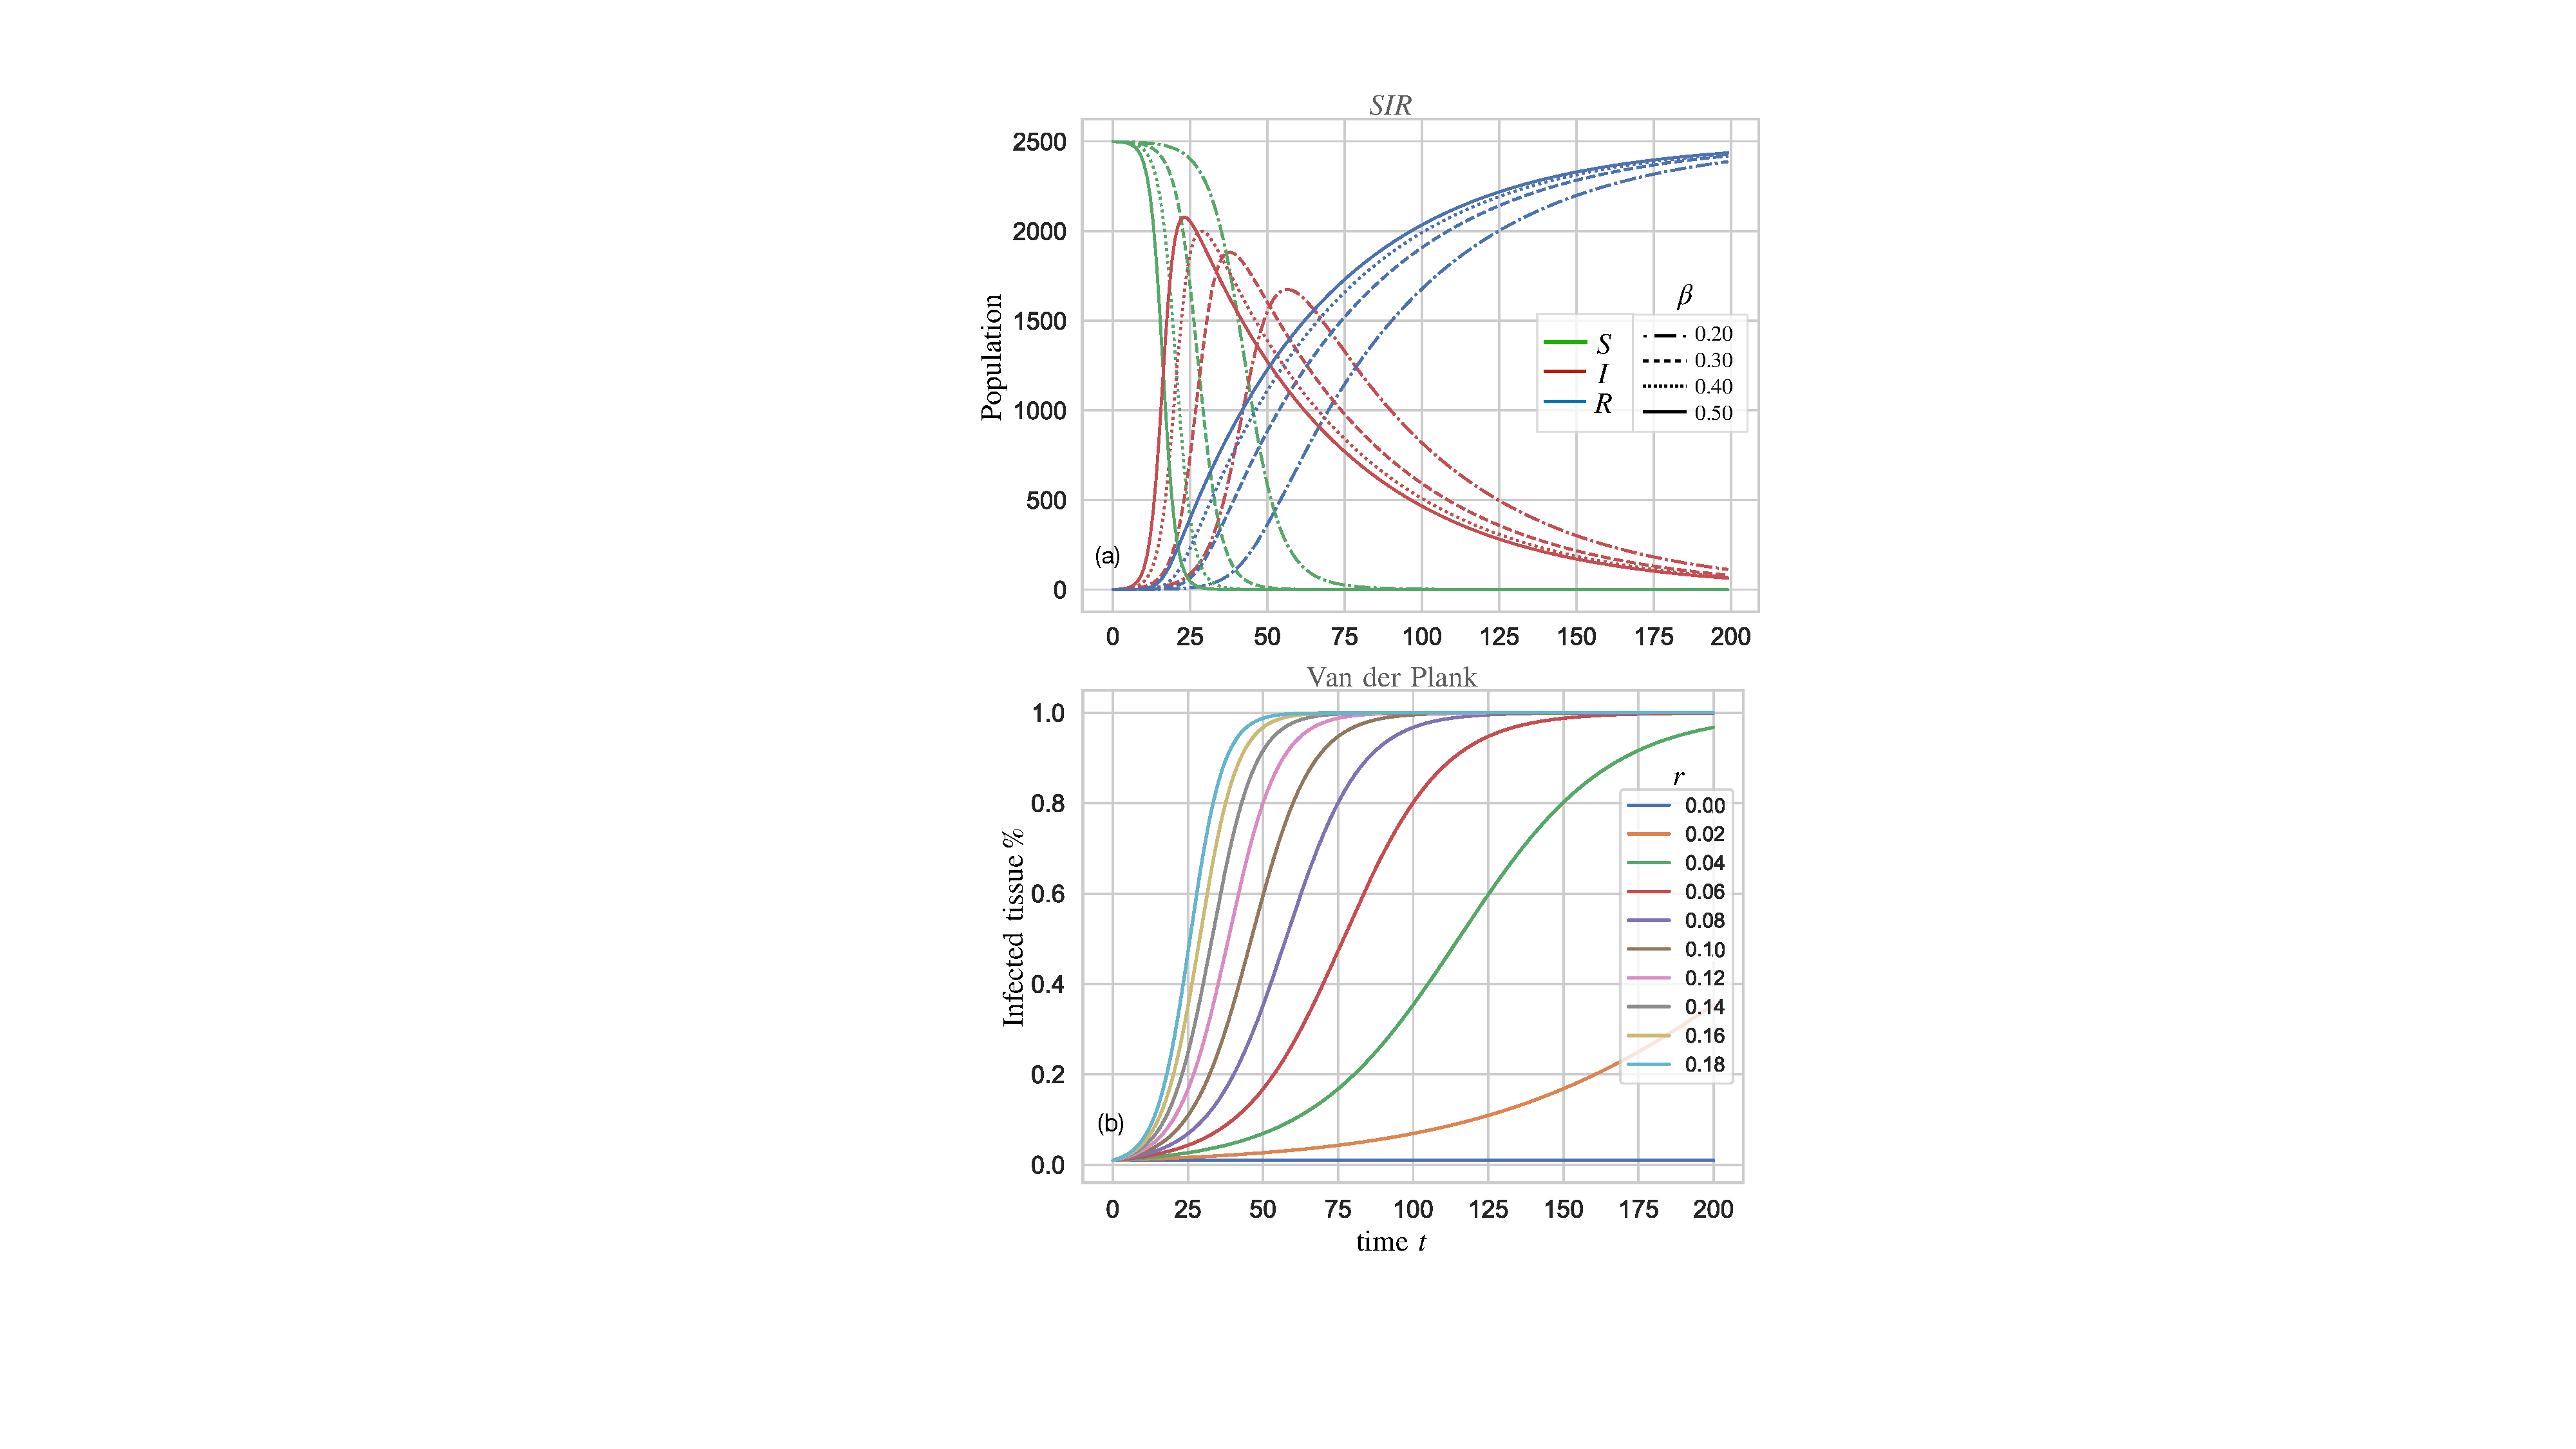
\includegraphics[scale=0.55]{chapter2/figures/SIR-vs-Plank.pdf}
     \caption{(a) The $SIR$ model as presented by \cite{kermack-model} is shown for fixed removal rate $\mu = 0.20$ and variations of $\beta$. 
                  The coupled system of ODEs can be solved numerically with Euler's method. Here, simulations begin with 
                  $2500$ susceptible and one infected individuals, and evolve for $t=200$ steps.
                  (b) The logistic growth model \cite{van2013plant} used to describe the growth of infected plant material.
                  Simulations are numerically computed with a forward-time finite difference method for $10$ different growth rates $r$.
       } 
     \label{fig:SIR-vs-plank}
 \end{figure}
where $r$ represents an `apparent' infection rate (measurable in laboratories from Equation \ref{eq:van-plank-r}),
and $R$ denotes the `basic' infection rate. As Plank explained, one usually seeks
to determine $R$ from the constant $r$. Assuming that $r$ indeed stays constant over the epidemic:
the basic infection rate $R$ must decrease as $x_t/x_{t-p}$ gets progressively smaller as $x_{t-p}\rightarrow x_t $.
At this point, the basic infection rate $R$ begins to resemble the effective reproduction ratio $R_e$
from Equation \ref{eq:R0-effective}. 

Equation \ref{van-plank-incubation} describes a system where
infections incubate for a period $p$ before inducing the growth of more infectious plant tissue.
However, it does not describe the infectious period (where infected tissue remains before becoming epidemiologically inert),
which lead Plank to extend Equation \ref{van-plank-incubation} to:
\begin{equation}
\label{van-plank-infectious-p}
    \frac{dI_t}{dt} = R_c(I_{t-p} - I_{t-i-p})(1 - I_{t})
\end{equation}
where $R_c$ is the basic infection rate `corrected' for removals and $i$ is the infectious period.
In this DDE, a unit of latently infectious tissue starts becoming infectious after $p$ steps, and stops becoming infectious $i$ steps.
More formally, as $I_{t-i-p} \rightarrow I_{t-p}$, the rate of infectious tissue growth approaches zero, $dI_t/dt \rightarrow 0$.

\subsection{Contrasting approaches}

The $SIR$ model does not include an incubation period, and therefore differs from the delayed differential formulation 
of Equation \ref{van-plank-infectious-p}. Nonetheless, the compartmentalised approach is easy to extend, leading to an 
$SEIR$ system:
\begin{align}
\label{eq:SEIR-model1}
    &\frac{dS}{dt} = -\beta SI \\
\label{eq:SEIR-model2}
    &\frac{dE}{dt} = \beta SI - \gamma E\\
    &\frac{dI}{dt} = \gamma E - \mu I \\
    \label{eq:SEIR-model3}
    &\frac{dR}{dt} = \mu I
\end{align}
where Equation \ref{eq:SEIR-model2} describes the population of latently (or exposed) infected hosts.
Susceptible hosts transition into the exposed compartment at the same rate as before, namely $\beta SI$, but now have an
exponentially distributed latency period of $\gamma^{-1}$ before transitioning into $I$.

Both Equations \ref{eq:SEIR-model1}-\ref{eq:SEIR-model3} and Equation \ref{van-plank-infectious-p} outline similar systems,
though infected tissue in Equation \ref{van-plank-infectious-p} remains infectious for precisely $i$ units.
This contrasts with the exponentially distributed exposed lifetime implicit within Equation \ref{eq:SEIR-model2}.
Nevertheless, \cite{segarra2001epidemic} illustrated how Plank's DDE and the $SEIR$ system are both special cases of
the $SIR$ model proposed by \cite{kermack-model}, when the $SIR$ model incorporates a sporulation function, $\phi(\tau)$. 
The sporulation function appropriately models spore production in plant pathogens. 
In particular, if $\phi(\tau) = 0$ for small $t$, $\phi(\tau)$ can model incubation periods. 
Similarly, if $\phi(\tau) = 0$  for large $t$, we recover an infectious period. 
More recently, \cite{time-varying-infectivity} simplified the analysis of \cite{segarra2001epidemic}, showing that 
both Plank's DDE and the $SEIR$ model can be recovered with an $SE_nI_mR$ model.
In an $SE_nI_mR$ framework, both $n$ and $m$ represent an arbitrary number of distinct exposed and infectious compartments:
\[
    S\rightarrow E_1 \rightarrow E_2 \rightarrow ... \rightarrow E_n \rightarrow I_1 \rightarrow I_2 \rightarrow ... I_m
\]
Trivially, the $SEIR$ model is recovered when $n=1$ and $m=1$. However, when $n,m \rightarrow \infty$,
\cite{time-varying-infectivity} demonstrated that we recover an expression equivalent to the DDE in Equation \ref{van-plank-infectious-p}.
Despite the sameness of both DDE and $SEIR$ formulations, the overarching theme of modern epidemiology is overwhelmingly compartmentalised,
owing to the increased flexibility and easier analysis of compartmental models.

\subsection{Progressive botanical epidemiology}
\label{sec:prog-epi}
After \cite{van2013plant} moved the field of botanical diseases into a more quantitative discipline,
theoretical investigations (alongside the adoption of computer simulations) characterised the next few decades.
Plank's DDE was applied to numerous pathosystems, halo blight in beans \cite{doi:10.1111/j.1744-7348.1979.tb06527.x} 
and grape powdery mildew \cite{sall1980epidemiology} to name a few. In particuar, \cite{sall1980epidemiology} adapted Plank's
logistic approach to include a time-varying infection rate $r(t)$. Moreover, diverse mathematical techniques, 
including multiple  regression analysis, were incorporated into mainstream plant epidemiology \cite{butt1974multiple}. 
Subsequently, \cite{zadoks1979epidemiology} consolidated various early mathematical models of plant disease 
alongside \cite{jeger1984use}.

Developments in computing compounded advances in plant epidemiology through this period. 
Improved accessibility and computer architectures permitted faster calculations and more intensive models. 
The first epidemic simulator (EPIDEM) written in FORTRAN IV came by \cite{waggoner1969epidem}. 
EPIDEM modelled the fungi `Alternaria solani' spreading through infected potato and tomato leaf tissue under different environmental conditions. 
    
An interesting early simulator (EPIMUL76) developed by \cite{zadoks1977role} adapted Van der Plank's logistic growth model into a spatio-temporal framework of two spatial dimensions. 
EPIMUL76 simulated the spread of disease on a two-dimensional domain, subdivided into $20\times 20$ host units referred to as `compartments', that took place inside a computer with $128\mathrm{K}$ of memory.
Arguably, subdividing the domain into separate compartments could be considered as an early agent-based model. 

In their analysis, \cite{zadoks1977role} alluded to the problem of scale in plant disease, as spatial scales
were conceptualised as `microscales' ($\leq 1\mathrm{m}$), `mesoscales' ($10^2\mathrm{m}$) and `macroscales' ($10^6\mathrm{m}$).
In this picture, microscales ranged from plant leaves to individual plants, mesoscales reflected crop fields, and macroscales
described large regional expanses over an entire country. Moreover, the probability of dispersal between infected hosts assumed a
Gaussian distribution\textemdash in contrast to \cite{doi:10.1146/annurev.py.06.090168.001201}.

In general, the ability to simulate more intricate models grew in proportion to the amount of computer memory available.
For a review of early plant disease simulators, see \cite{doi:10.1146/annurev.py.23.090185.002031}.

\subsection{Percolation: from forest fires to epidemics}
\label{section:lit-rev-perc}

Research on percolation occurred alongside the developing field of plant disease modelling.
The development of percolation theory marked an early approach to modelling epidemic systems that are
both spatially-explicit and stochastic.
The original formulation of percolation theory was first used to describe properties of a fluid and the 
bonds which form between molecules \cite{perco_origin} (a more formal account of 
percolation is undertaken in section \ref{ch3:invasions_and_persistence}). The problem was posed on a 
graph\textemdash illustrated in terms of vertices and edges. However re-interpretations were subsequently 
put forward by physicists studying material sciences, naturally on a lattice. \cite{Essam_1980}. 
The attractive feature of this new paradigm was that percolation demonstrated a phase-transition. 
Thus, percolation could be treated with scaling theory used in the study of critical-phenomena. 
Accordingly, early work rigorously ensued to map out the behaviour of percolation around criticality in 
terms of critical exponents \cite{STAUFFER19791}. 

Different flavours of percolation models, such as site or bond percolation, were described
to model different processes. Nevertheless, percolation proved a convenient theory and various phenomena including gelation, 
magnetism and telecommunications were described \cite{trove.nla.gov.au/work/26493727}. In particular, 
forest fire models were related to percolation \cite{MacKay_1984}, 
with only a short conceptual jump from time-dependent percolation used to study the growth of crystals \cite{Family_1985}. 

A fire spreading through a population of trees is not too different to a disease spreading through 
a population, thus leading to a general epidemic-formalisation within a percolation-based framework
\cite{pub.1059067807}; the researchers proposed that epidemics might be in the same universality class
as percolation. Beginning with a simple $SIR$ framework put forward by \cite{kermack-model}, the field 
of epidemiology was already well-established around the time percolation theory was conceived \cite{baily1975mathematical}. 
Naturally, percolation models could relax assumptions about population mixing and serve as a helpful tool
when developing spatially structured epidemic models.

A fractal-like pattern of epidemics was observed by \cite{GRASSBERGER1986273}, shown in Figure \ref{fig:1d_perc_basis}. 
In Figure \ref{fig:1d_perc_basis}, lighter grey sites represent removed individuals, 
black sites indicate actively infected sites, and white sites indicate unaffected sites. 
All lattice sites in the bottom row were initially infected, and the infection can be seen to propagate
from the bottom up. The lattice was initialised at the critical-density $p\sim p_c$ culminating in a fractal-like pattern.
\cite{GRASSBERGER1986273} did not attribute the hosts of this model to be trees, but instead a general host-population with low mobility. 
The authors noted that local interactions between hosts and infected were vast simplifications and proposed 
generalising the system with long-range interactions following a power law. 
Although, it must be remarked that including long-range interactions would cease to describe a percolation based system.

\begin{figure}
    \centering
    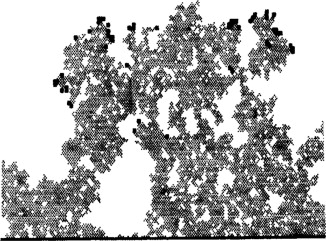
\includegraphics{chapter2/figures/perc1.jpg}
    \caption{A space-time representation of an epidemic spreading at the critical threshold. 
    The spatial (horizontal) and time (vertical) axis show self-similar propagation of diseased 
    individuals in grey, produced by \cite{GRASSBERGER1986273}}
    \label{fig:1d_perc_basis}
\end{figure}

Percolation models of epidemics were investigated by several means, 
e.g. renormalisation-groups \cite{pub.1060474189} and Monte-Carlo methods \cite{pub.1059069981}. 
Studies generally focused on finding the systems critical exponents and categorising phase
transition graph that characterised an epidemic (super-critical) or extinction (sub-critical) 
regimes \cite{GRASSBERGER1986273}. The properties of both epidemics and forest fire percolation 
models were studied together in \cite{pub.1052857560}, highlighting their similarity.
One of the first ecological applications was put forward by \cite{pub.1031591030}, 
who studied the effects of landscape distributions and percolation models 
(reflecting both forest fire and epidemics). In their study, \cite{pub.1031591030} 
combined $SIR$-like mechanics inside a percolation-based distribution of hosts and subsequently 
found a narrow regime where disease epidemics would spread, thus mirroring the threshold-like 
behaviour witnessed in the $SIR$ model. Although, here, the authors considered the possibility of host recovery.
% \textemdash \cite{GRASSBERGER1983157} <- reference for early considerations towards percolation as a model for tree diseases and percolation
% \textemdash \cite{SANDER2002293}, read and get more info + research links
\newpage

\section{Spatially-explicit epidemic models}
\label{ch2:lit-rev-compartmentalised-models}

Emergent infectious diseases (EIDs) in tree populations are multi-scale,
they can span regional, country or continental spatial scales. Considerable variations in landscape composition,
tree densities, population aggregation, and the climatic factors give rise to diverse spatio-temporal
patterns of disease spread \cite{he2019integrating, suzuki2003spatial}. Incorporating spatial structure
in tree-disease models is therefore vital to accurately capture the environmental influences upon host-pathogen 
interactions and dispersal \cite{liu2007characterizing}. This section outlines several approaches to modelling
the spread of tree disease.

\subsection{Small-scale: stochastic dispersal}
\label{ch2:dispersal}

Pathogen dispersal through wind, watercourse or human trade underpins a key feature of EDIs. 
Numerous functions have been used to model dispersal, but generally, all describe a continuous 
non-negative (real-valued) function that is normalisable: $\int_{-\infty}^{\infty}  D(x)dx = 1$.
Various review articles provide comprehensive functional examples \cite{bullock2017synthesis, nathan2012dispersal, howe1982ecology}; 
however, the general class of dispersal kernels include thin-tailed Gaussian and 
exponential alongside fat-tailed inverse power law variants.

Early plant disease simulators (e.g. EPIDEM and EPIMUL76) included stochastic dispersal\textemdash 
discussed at length in section \ref{sec:prog-epi}. A more recent article by \cite{parnell2010effect} 
modelled stochastic dispersal in Citrus canker to investigate the effects of landscape aggregation 
patterns and disease progression.
\cite{parnell2010effect} studied landscape patterns of two kinds: 
1) varying degrees of randomly distributed densities 
2) varying degrees of host aggregation.
The epidemic model was based on a series of prior Citrus canker works
\cite{parnell2009optimal, gilligan2008epidemiological, cook2008constructing}.
The epidemic model is described by:
\begin{equation}
\label{eq:prob-trans}
    Pr(S_i \rightarrow I_i)_{\Delta t} = 1 - \exp\big[- \beta \sum_j^N\exp^{-\alpha d_{ij}} + \epsilon \big]
\end{equation}
Here, a transition probability describes the $i^{th}$ susceptible tree becoming infected 
during the step $t \rightarrow t + \Delta t$ on account of $N$ infected trees.
Equation \ref{eq:prob-trans} assumes that dispersal exponentially decreases with distance (i.e. $\exp^{-\alpha d_{ij}}$), 
where $\alpha$ denotes the dispersal scale parameter. Infection pressure from the $j^{th}$ infected tree is multiplied by an
infection rate, $\beta$. The last parameter to consider in Equation \ref{eq:prob-trans}
is the primary infection rate $\epsilon$. The primary infection rate reflects the chance of infection from sources outside
the immediate system, i.e. at time $t=0$, distant infected populations external to the
closed host population under consideration.

The outside exponential term of Equation \ref{eq:prob-trans} depicts a cumulative exponential threshold above which 
trees become infected. Interestingly, this threshold is based on the `Skelle construction' \cite{sellke1983asymptotic}. 
More specifically, Skelle assumed that susceptive hosts need an arbitrary (cumulative) degree of infection
exposure before becoming infectious. Using Equation \ref{eq:prob-trans}, \cite{parnell2010effect} proceeded to define 
a control radius and found that both landscape aggregation and (randomly distributed) high host densities increase the
optimal control radius. 

A later paper by \cite{WEBIDEMICS} proceeded to generalise the Citrus canker model.
Primarily, the authors examined an $SECIR$ model\footnote{
Here, compartments are (S)usceptible, (E)xposed, (C)ryptic and (R)emoved) where $C$ 
denotes unobservable cryptic infections.}, though several other model variants were included. 
\cite{WEBIDEMICS} contrasted both Gaussian and Cauchy dispersal kernels.
Cunniffe et al. included dispersal parameters provided by \cite{neri2014bayesian}, who
assessed Cauchy kernels\textemdash in addition to exponential kernels.
The general model followed:
\begin{equation}
\label{eq: webidemics}
     \phi_i(t) = w(t)\big[\beta \sum_j K(d_{ij}; \alpha) + \epsilon \big]
\end{equation}
where $w(t)$ is a time-dependent infectivity function, $\epsilon$ is the primary infection 
(set to zero in the manuscript), $\beta$ is the rate of secondary infection, and $K(d_{ij}; \alpha)$
is the dispersal function. This time, Equation \ref{eq: webidemics} presents a rate of transition for a single
susceptible tree (from $S_i \rightarrow E_i$) under the influence of all infected neighbours (represented by the $j^{th}$ index),
as opposed to the probability of Equation \ref{eq:prob-trans}.

Cunniffe et al. examined the effects of a cull radius, similar to \cite{parnell2010effect}. 
However, this time, results were aimed towards assessing control when there is epidemic uncertainty.
Consequently, \cite{WEBIDEMICS} assessed different epidemic serveries by varying $\beta$, alongside
numerous control parameters, e.g. eradication response time, detection probabilities and revisit/survey intervals. 

All in all, \cite{WEBIDEMICS} highlighted an intuitive result, namely, that the scale of control should
reflect the "intrinsic epidemic scale". More succinctly, \textit{aggressive pathogens should be met with 
an aggressive control strategy}. Moreover, Cunniffe et al. suggested that thick-tailed dispersal kernels
(in this case, a Cauchy distribution) prove more challenging to control.

The Citrus canker models developed in Equations \ref{eq:prob-trans} and \ref{eq: webidemics} 
contrast with non-spatial analytical systems. For example, the model of pine wilt disease (PWD)
constructed by \cite{khan2020modelling}, who coupled a differential system of pine (H)osts and beetle (V)ectors 
following:
\begin{align}
    \label{eq:PWD-model1}
    &\frac{dS_H}{dt} = \lambda_H - \beta_1\Psi S_H I_V - \beta_2\Phi\alpha S_H I_V - \gamma_1 S_H \\
    &\frac{dE_H}{dt} = \beta_1\Psi S_H I_V - \beta_2\Phi\alpha S_H I_V  - (\gamma_1 + m)E_H \\
    &\frac{dA_H}{dt} = m(1 - \omega)E_H - \gamma_1 A_H \\
    \label{eq:PWD-model-H}
    &\frac{dI_H}{dt} = m \omega E_H - (\gamma_1 + \mu ) I_H \\
    \label{eq:PWD-model-V}
    &\frac{dS_v}{dt} = \lambda_V - K S_v I_H - \gamma_2 S_V \\
    &\frac{dE_v}{dt} = K S_v I_H - (\gamma_2 + \eta) E_V \\
    \label{eq:PWD-model7}
    &\frac{dI_v}{dt} = \eta E_V - \gamma_2 I_V
\end{align}
In this system, pine tree hosts interact with beetle vectors that carry pathogenic nematodes 
(\textit{Bursaphelenchus xylophilus}). Stepping through the system:
Equations \ref{eq:PWD-model1}-\ref{eq:PWD-model-H} describe the host population;
births and naturally occurring deaths in the host population occur at rates $\lambda_H$ and $\gamma$, 
respectively. Pine trees become infected by two mechanisms: $\beta_1\Psi$ that describes the incidence
rate with infected mature beetles, and $\beta_2\Phi$ that describes the incidence rate with beetle offspring.
Once pine hosts become exposed, a fraction ($\omega$) transition into the infectious symptomatic state $I$, 
while the remaining fraction ($1 -\omega$) become asymptomatic\textemdash both pathways occur at rate $m$. 
Disease induced death happens at a rate $\mu$. Equations \ref{eq:PWD-model-V}-\ref{eq:PWD-model7} outline a 
($SEI$) dynamic for beetle vectors. Natural births and deaths in the beetle population happen with rates 
$\lambda_V$ and $\gamma_2$, respectively. Furthermore, susceptible beetles become exposed by feeding infected
hosts at rate $K$ and transitioning into the infected beetle class at rate $\eta$.

Equations \ref{eq:PWD-model1}-\ref{eq:PWD-model-H} assume mass action population mixing of beetles 
without stochasticity. Presumably, this assumption led \cite{khan2020modelling} to model PWD as a non-spatial
system on account of the migratory population of Beetle vectors. In reality, a dispersal kernel is likely to 
describe beetle movements more accurately than the well-mixed system presented in Equations 
\ref{eq:PWD-model1}-\ref{eq:PWD-model-H}. Case in point, the spatio-temporal dynamics of Asian longhorned
beetle was examined by \cite{smith2004dispersal} who inferred a median dispersal rate of $30\mathrm{m/day}$
according to an exponential dispersal kernel (with only $2\%$ of beetles exceeding $920\mathrm{m}$).
Linear stability analysis was performed on the deterministic system of Equations \ref{eq:PWD-model1}-\ref{eq:PWD-model-H}. 
Whereas the stochastic spatio-temporal framework of Equations \ref{eq:prob-trans} and \ref{eq: webidemics} 
were analysed by repeating simulations inside an ensemble.

% \begin{itemize}
%     \item The importance of dispersal
%     \item How is dispersal treated mathematically ?
%     \item What type of dispersal kernels have been studied?
%     \item What parameter-values have been inferred ?
%     \item How long-range can dispersal be ? Talk about long-range inter-Continental dispersal
%     \item see \cite{nathan2012dispersal} for a review of dispersal kernels
% \end{itemize}


\subsection{Large-scale}
% -\cite{doi:10.1098/rstb.1986.0072}
% -item \cite{large-scale-control}

Ultimately, microscopic (host-pathogen) interactions propagate the spread of disease. 
Although once disease-establishment has taken place, large-scale outbreaks can spread through vast
areas, e.g. the spread of ash dieback through Europe \cite{alsop2015ash}.
As a result, contemporary modes of tree disease have examined the large-scale spread over entire landscapes.
The previous section outlined some small-scale models (on the order of $1 \sim 10 \mathrm{km}$), 
however, in this section, we focus on large-scale epidemic models.

Over large scales, disease drivers include long distance dispersal (LDD) through wind \cite{golan2017long, gross2014h} and
trade \cite{ash-dieback-costs, perrings2016options, harwood2009epidemiological, doi:10.1098/rsif.2005.0051}.
However, linking human trade networks and dispersal in one large-scale model is challenging due to numerous complex parameters 
and epidemiological drivers. 

A framework constructed by \cite{harwood2009epidemiological} incorporated the growth and reproduction, dispersal and trade
of infectious plant material into a single model. The study conducted by \cite{harwood2009epidemiological} aimed
to assess the risk of \textit{Phytophthora ramorum} and \textit{Phytophthora kernoviae} in the UK by
employing a linked network approach. 
In the linked network, single grid cells of area $\mathrm{1km \times 1km}$ were coupled together by a (wind-borne)
dispersal kernel and a trade network. 
Following earlier earlier work \cite{madden2007study}, the population inside each grid cell evolved according
to an $SEIS$ model:
\begin{align}
    \label{eq:phyt-model1}
    &\frac{dS}{dt} = \mu E + \mu I - \beta S i\\
    &\frac{dE}{dt} =  \beta S i - k E - \mu E   \\
    \label{eq:phyt-model3}
    &\frac{dI}{dt} = k E - \mu I
\end{align}
where host introductions were assumed to balance the total number of removals $\mu (S + E + I$).
Then, dispersal between $\mathrm{1km \times 1km}$ grids took place inside a domain of size $\mathrm{700km \times 1300km}$ 
covering the UK. Here, the host population was informed by the Country side survey data\textemdash discussed more 
below in section \ref{ch2:hostdata}. An inverse square power law described wind-borne dispersal (with a scale constant
of $2\mathrm{m}$), though parameterisation was qualitative and uniformed by experimental data.

In addition, a simulated trade network linked $\mathrm{1km \times 1km}$ cells. 
In the trade network, plant nurseries and retailers were connected by LDD trade and transport. 
In this manner, \textit{Phytophthora ramorum} and \textit{Phytophthora kernoviae} could jump 
between cells. The same linked-network approach was later used to reconstruct the highly 
popularised 1970s Dutch elm disease epidemic in Great Britain \cite{doi:10.1111/j.1365-3059.2010.02391.x, potter2011learning}.

A similar construction was put forward by \cite{meentemeyer2011epidemiological} to 
forecast the spread of sudden oak death (SOD) in California from (1990-2030).
A distribution of host\footnote{In this context, `host' refers to a wide-range
species susceptible to \textit{P. ramorum} \cite{tooley2004susceptibility}.
} abundance was derived from previous SOD modelling work 
\cite{meentemeyer2004mapping} and comprised $\mathrm{250 \times 250}$ grid cells
weighted by the relative susceptibility to \textit{P. ramorum} from 1-100. As a result,
a high-resolution map of `host index' was produced throughout the state of California.

The large-scale SOD model included several epidemiological drivers of \textit{P. ramorum}: 
forest-type, local weather conditions, oak density, local pathogen growth and transmission
and longer-range transmission. Local-scale dispersal were estimated
using Markov chain Monte Carlo (MCMC) methods from aerial surveys \cite{valachovic2008wildland} 
of \textit{P. ramorum}, and positive sites (2001–2007) confirmed by the California Department of
Food and Agriculture were used to estimate the long-range dispersal. \cite{meentemeyer2004mapping}
found that a long-range Cauchy distribution fitted the data most appropriately over both spatial scales.
Hence, a multi-scale kernel was given as:
\begin{equation}
\label{eq:multi-scale-kernel}
    K(d; \alpha_1, \alpha_2, \gamma) = \gamma( 1 + (d/\alpha_1)^2 )^{-1} + (1 - \gamma)( 1 + (d/\alpha_2)^2 )^{-1}
\end{equation}
where $\alpha_1 = 20.57\mathrm{m}$ and $\alpha_2 = 9.5\mathrm{km}$ represent the short and long range dispersal
kernels respectively, and the ratio $\gamma=0.99$ estimates the total contribution to short and
long-range dispersal. Using the multi-scale dispersal kernel in Equation \ref{eq:multi-scale-kernel},
the epidemiological model between $\mathrm{250 \times 250}$ grid cells assume the form:
\begin{equation}
\label{eq:large-scale-model}
    \Psi_{ijt} = \beta \sum_i \big(\chi_t (f_i) m_{it} c_{it} I_{it} \big) \big( \chi_t(f_j) m_{jt} c_{jt} S_{jt} /N_{max} \big) \times K(d_{ij}; \alpha_1, \alpha_2, \gamma)
\end{equation}
where $\Psi_{ijt}$ represents the infection pressure from grid $i$ to grid $j$ in one week $t$ intervals. 
Equation \ref{eq:large-scale-model} includes multiple component-functions and parameters: 
\begin{itemize}
    \item A binary-valued function $\chi_t(f_i)$ that indicates if forest type $f_i$ can infect and become infected at time $t$
    \item two indices $m_{it}$ and $c_{it}$ that indicate moister and temperate of patch $i$ at time $t$
    \item $I_i$ and $S_j$, the number of infected in grid $i$ and susceptibles at $j$
    \item $K(d_{ij})$, the dispersal kernel from Equation \ref{eq:multi-scale-kernel}
    \item $\beta$ that models the rate of spore production per site per week.
\end{itemize}

From the model, \cite{meentemeyer2004mapping} predicted which areas in California
had the highest secondary infection risk of SOD over $40$ years.
Simulations were ensemble-averaged based on predicted weather conditions from 2008–2030.
Climatic variations were classified as `favourable', `random' and `unfavourable'.
In all variations, SOD was predicted to spread through California and effect $1000$s
of square kilometers. However, considerable spatial and temporal variation were witnessed
across different Californian states. Additionally, \cite{meentemeyer2004mapping} 
observed that $93\%$ of short-range dispersal occurred within the range of a single $\mathrm{250 \times 250}$ and 
$95\%$ of infrequent long-range spread remain within $100\mathrm{km}$ in their model.
Although, most dispersal remained localised $<1\mathrm{km}$.

The manuscript authored by \cite{meentemeyer2004mapping} emphasises the multi-faceted 
parameters and processes that one needs to consider before modelling a large-scale epidemic
outbreak; these included, host data, dispersal, and climate.
\cite{large-scale-control} subsequently extended the analysis of \cite{meentemeyer2004mapping}
to assess the large-scale effects of epidemic control. 
In particular, \cite{large-scale-control} examined how to optimise eradication of SOD with 
limited resources. When resources are low, the authors suggested that small localised 
eradication zones around \textit{known} foci optimise control; justified by the fact that
small, but more numerous, control areas about diseased areas reduces the risk of failing 
to treat a high-risk site that causes many secondary infections. 

\cite{large-scale-control} also tested management strategies based on targeting:
1) hosts irrespective of disease 
status (the "host" strategy)
2) local areas with high prevalence ("hazard" strategy)
3) areas with high basic reproduction numbers ("susceptible" strategy)
4) regions ahead of the wavefront ('wavefront" strategy).
Of all the management scenarios tested, \cite{large-scale-control} found
that 4), treating areas ahead of the wavefront, reduced epidemic spread the most.
In this scenario, the affected area was reduced by $\sim 2400\mathrm{km^2}$ and 
the optimal culling radius was determined to be $362.5\mathrm{m}$.

All the large-scale models discussed above split the population into smaller (sub)girds.
As such, they share noticeable similarities to a metapopulation\footnote{
Metapopulation dynamics generally aim to deconstruct a spatial population into separate sub-populations contained within a `patch'. Then, between-patch interactions aim to model population migrations, connectedness and fragmentation, while within-patch
dynamics aims to model colonisation, persistence, competition, coexistence, and habitat suitability.} commonly used by ecologists studying spatially-structured animal and plant populations \cite{hanski1998metapopulation}. 
However, plant-disease modellers increasingly utilise metapopulation settings to study the effects of landscape features on disease progression, e.g. \cite{beninca2020trade, soubeyrand2009spatiotemporal, doi:10.1046/j.1461-0248.2002.00378.x}.
 
% WORK IN PROGRESS
%     \item  \cite{https://doi.org/10.1111/jbi.13642}
%     \item  \cite{pautasso2013european}, search for 'modelling' in this review paper. It contains references to LDD models.
%     \item LDD is an important factor of the scale of spread. Long distance dispersal has been considered for many biological processesd distance between patches can...


\subsection{Disease fronts}

\blindtext

\blindtext

\begin{figure}
    \centering
    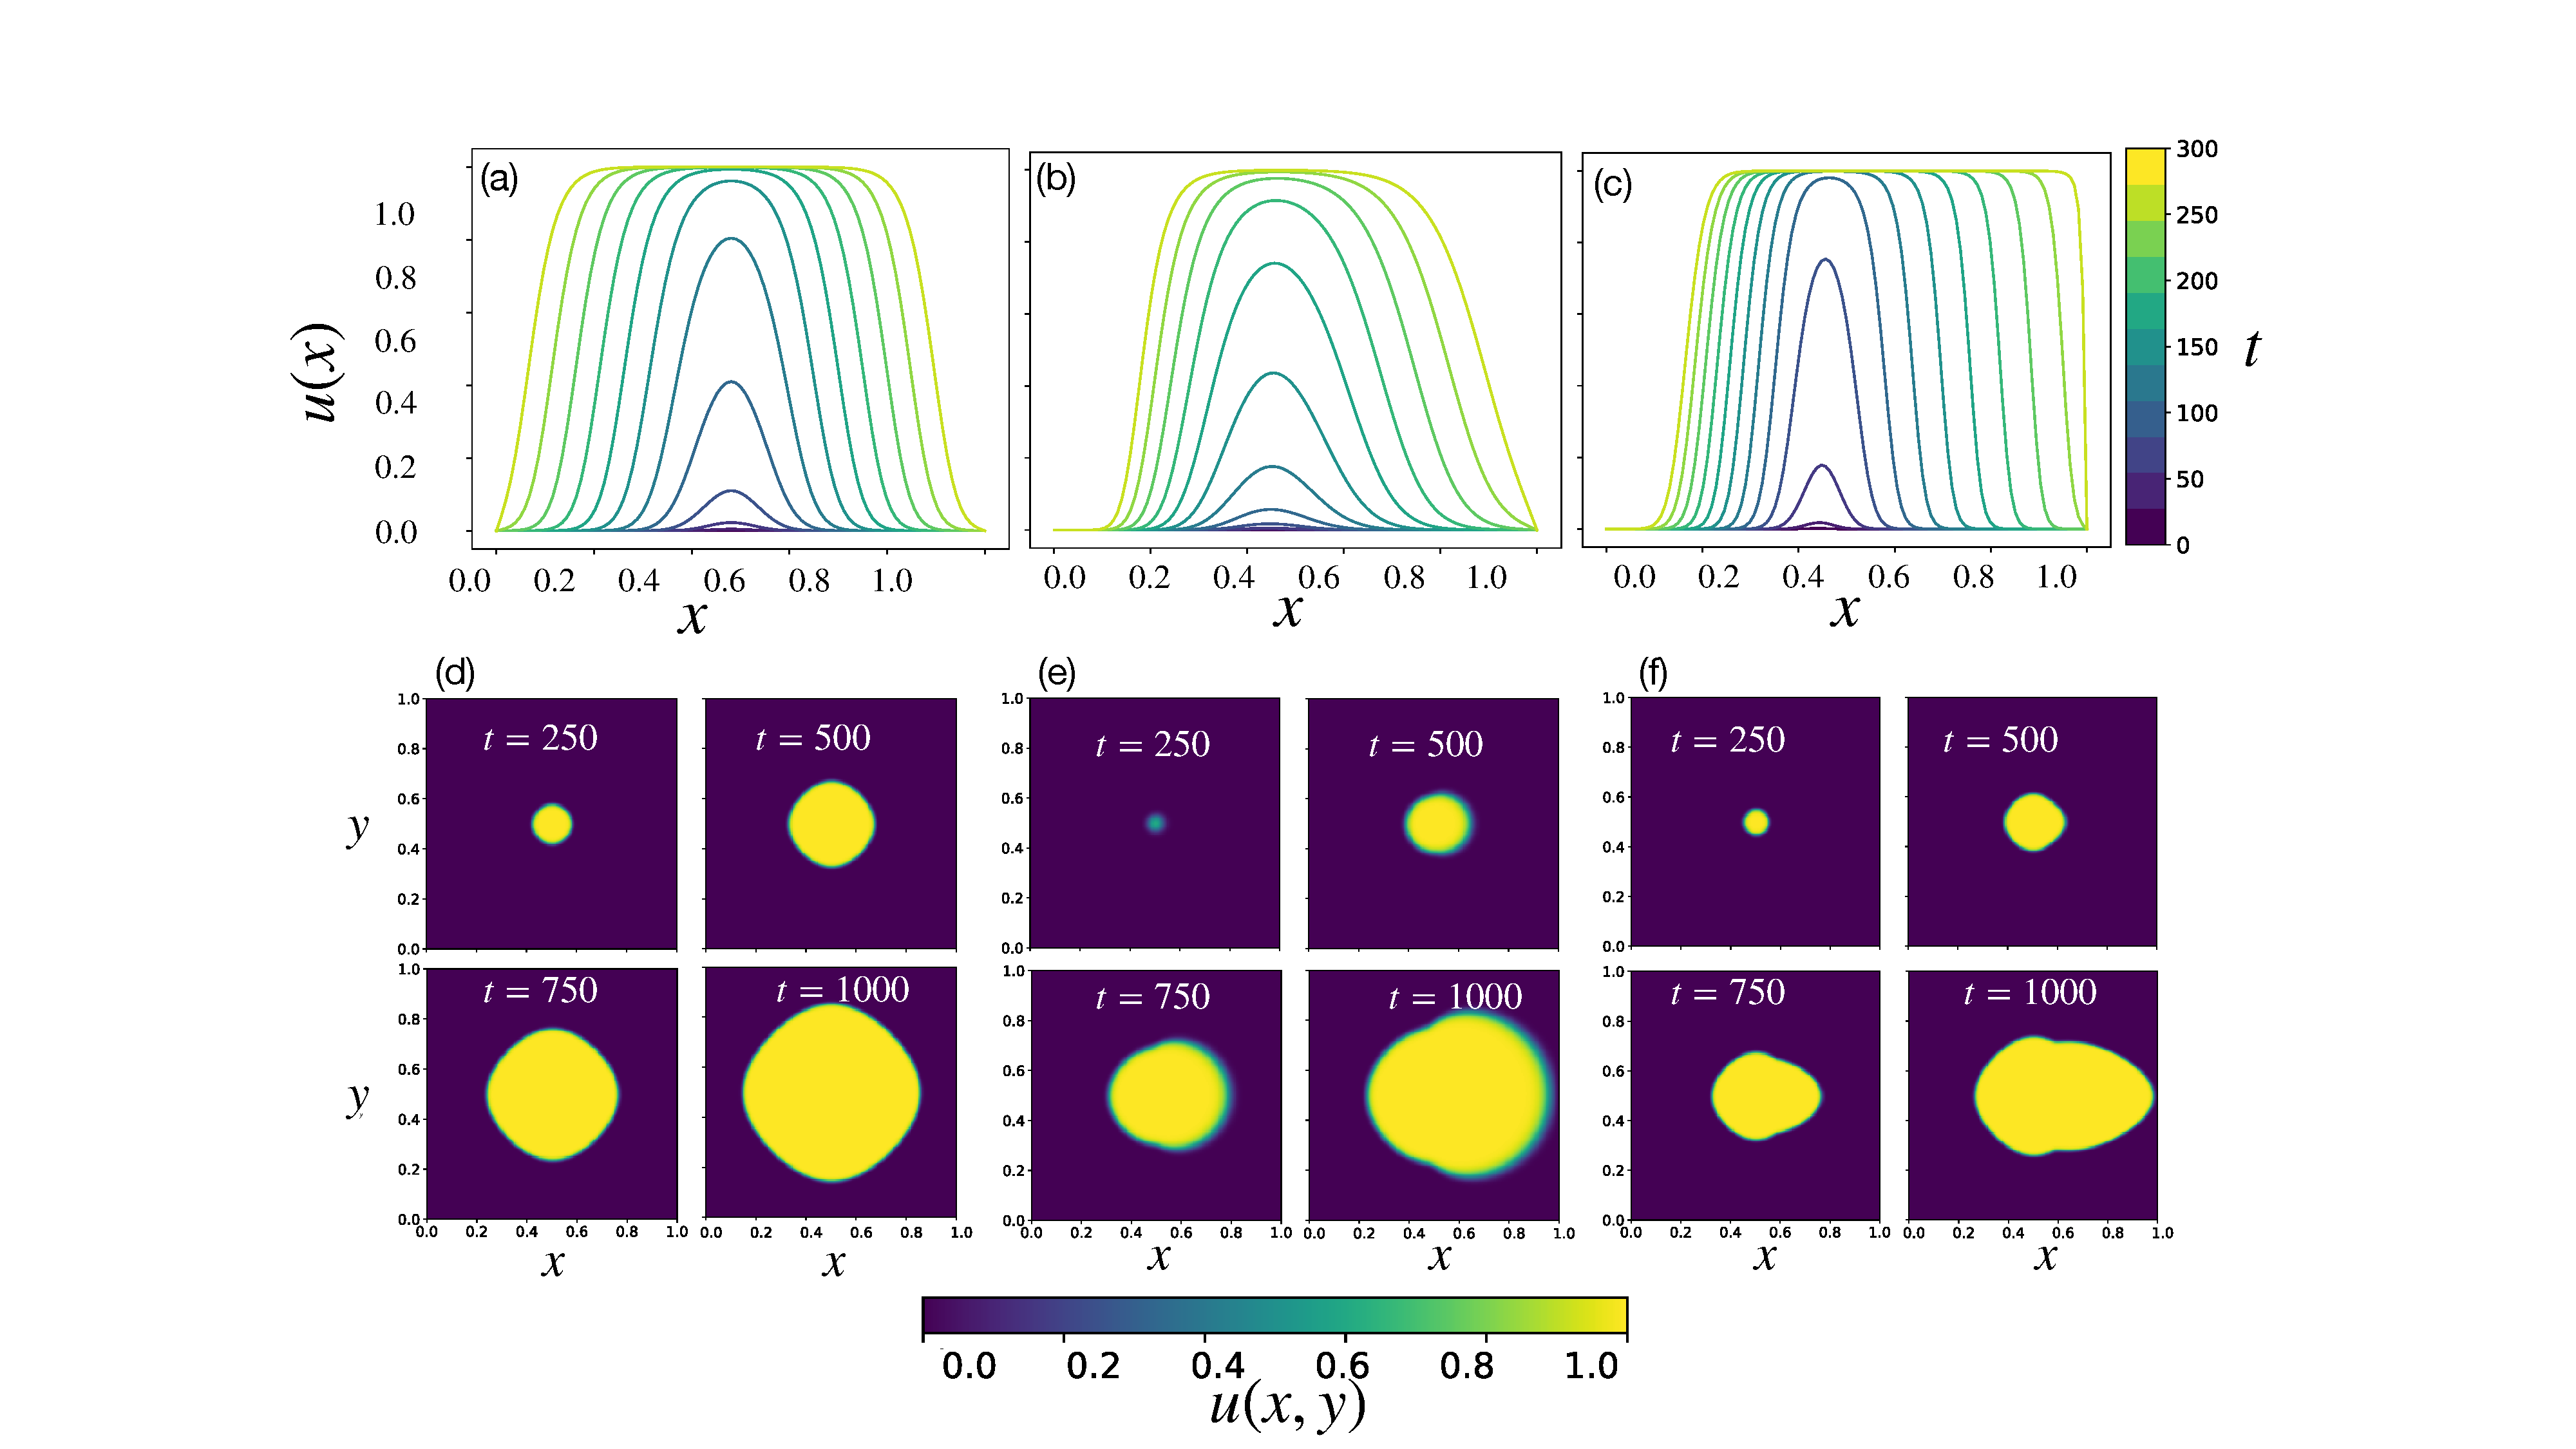
\includegraphics[scale=0.325]{chapter2/figures/FKPP.pdf}
    \caption{
    A simulations of the FKPP model for $r=0.10$ and $\mathcal{D}=0.10$ in one spatial dimension. 
    A non-zero field value is initialised at $x=10$ at time $t=0$. Uniform growth and diffusion 
    give rise to a wave-front that propagates with constant speed.}
    \label{fig:fkpp-expo1D}
\end{figure}

\blindtext


% initially travelling waves... 
% describe FKPP...
% power law dispersal... \cite{severns2019consequences} accelerating fronts...


% \textcolor{red}{
% \begin{itemize}
%     \item review \cite{doi:10.1098/rsif.2005.0051}
% \end{itemize}}

% \subsection{Diffusion}

% \cite{mundt2009long}  \cite{mundt2009aerial}

% In one spatial dimension, the FKPP model is given by:
% \begin{equation}
%     \frac{\partial u}{\partial t} = \mathcal{D}\nabla u + ru(1 - u/K)
% \end{equation}
% where $\mathcal{D}$ is a diffusion coefficient measured in units $\mathrm{m^2 t^{-1}}$ 
% and $r$ is a growth constant (or rate) with units $t^{-1}$. 
% This model assumes logistic growth and diffusion, where the field $u$ represents a `concentration',
% and $K$ represents the carrying capacity, when $u=K$, the system growth goes to zero.

%\item \cite{doi:10.1098/rstb.1998.0226} gave a three population (host, parasite and hyperparasite), which considered transmission via a reaction-diffusion process.

% \textcolor{red}{
% \begin{itemize}
%     \item Spatial SIR model
%     \item Agent-based modelling
%     \item A good place to talk about Percolation models
%     \item \textcolor{red}{Murray}: travelling waves that do not change shape
% \end{itemize}}

\section{Tree distribution datasets in Great Britain}
\label{ch2:hostdata}

Large-scale epidemic models of tree disease rest on robust, high-quality host data.
Data-driven approaches are crucial for predicting disease spread over country-wide scales, 
though collecting high-quality host data involves myriad challenges. 
Most notably, large-scale species distributions require vast datasets that demand significant economic resources
and person-hours to assemble and maintain over time. 
However, satellite-based remote sensing technologies pose an attractive solution\textemdash see \cite{camarretta2020monitoring} for a recent review of remote sensing technologies.
Despite the significant advances of remote sensing technologies, most freely available data sets still rely on traditional surveying methods to collect data throughout Great Britain (GB).
Consequently, the most widely known and widely used datasets are reviewed below.
Following this, statistically-generated species distribution models, typically based on surveyed data, are reviewed.

\subsection{National Surveys}

Surveyed data predominantly describes either: abundance, presence-only, presence-absence data. 
Generally, abundance data describes percentage canopy cover per $\mathrm{km^2}$.
In contrast, presence-only and presence-absence data that record if a species is present or present and absent, respectively.
Abundance captures significantly more information than presence-only data, yet unfortunately, they are in short supply.

\subsubsection{Countryside Survey}

The countryside survey (CS) is a long-running, national survey of diversity and species abundance in GB \cite{wood2017long}.
The UK Centre of Ecology and Hydrology (UKCEH) undertakes the surveys, primarily funded by the Natural Environmental Research Council alongside other government agencies.
Individual surveys have been undertaken in: $1978$, $1990$, $1998$, $2007$, and $2019$. 
Random stratified sampling captures a representative species abundance\footnote{
A useful (unpublished) project merged abundance data from CS with myForest. The abundance data can be found at the Oxford University research archive: \nolinkurl{https://ora.ox.ac.uk}.} 
over of all land cover compositions, e.g. lowland acid grassland, freshwater, and broad-leaf forest.

Abundance data is collected for numerous dominant species, including trees, shrubs, ground flora and soil type, 
making the scope of CS data vast. Moreover, long-running records spanning decades reveal ecosystem trends imperative for ecological monitoring.
More recently, $100$ $1\mathrm{km^2}$ plots of vegetation and soil data were collected\footnote{
The data is free to download on the UKCEH website: \nolinkurl{https://catalogue.ceh.ac.uk}} \cite{10.5285/fd6ae272-aeb5-4573-8e8a-7ccfae64f506}.
The dataset constitutes the first of five planned surveys, part of a rolling monitoring strategy collected every five years.

\subsubsection{National Forest Inventory}

\begin{figure}
    \centering
    \includegraphics[scale=0.2]{chapter2/figures/NFI-figure.pdf}
    \caption{NFI data super imposed onto a Google earth image, taken from a report (unpublished) by S. Orozco-Fuentes et al.
             NFI data covering Thetford Forest Park ($16.684 \mathrm{km}^2$) is shown as a polygon in the NFI `woodland' category.
             Data is interpreted as the conifer forest type. Here, surveys comprises presence-only data, and no tree species percentage cover
             is reported. NFI data extends throughout $\sim 13\%$ of land coverage in GB and large non-woodland areas remain un-surveyed.}
    \label{fig:NFI-data}
\end{figure}

The National Forest Inventory (NFI) collects and maintains forest and woodlands data in GB.
Originally, the NFI was established to help restore and expand Britain's woodlands following the First World War \cite{james1990history}.
Regular programs ($10$-$15\mathrm{year}$ intervals) implement surveys of woodland and forest size, distribution, composition and condition across GB.
Records cover areas over $0.5\mathrm{ha}$ and $20\%$ coverage.
As of $2019$, $622,381$ individual records exist, spanning $2.9 \times 10^6 \mathrm{ha}$ over $13\%$ of the total land cover within GB.
NFI data comprise ESRI shape files\footnote{
Free to download at: \nolinkurl{https://data-forestry.opendata.arcgis.com}},
that outline numerous forest types, e.g. broadleaved, conifer, mixed-predominantly broadleaved or mixed predominantly conifer.
Despite an extensive coverage, publicly available NFI surveys describes presence-only data\textemdash with no proportion or species coverage.
Although, additional datasets are available to purchase, including: 
1) Tree species percentage per region by woodland type
2) Tree species proportions within the upper canopy of each NFI sample plot, without supplying the exact location of the individual sample plot.

\subsubsection{Botanical Society of Britain and Ireland}

\begin{figure}
    \centering
    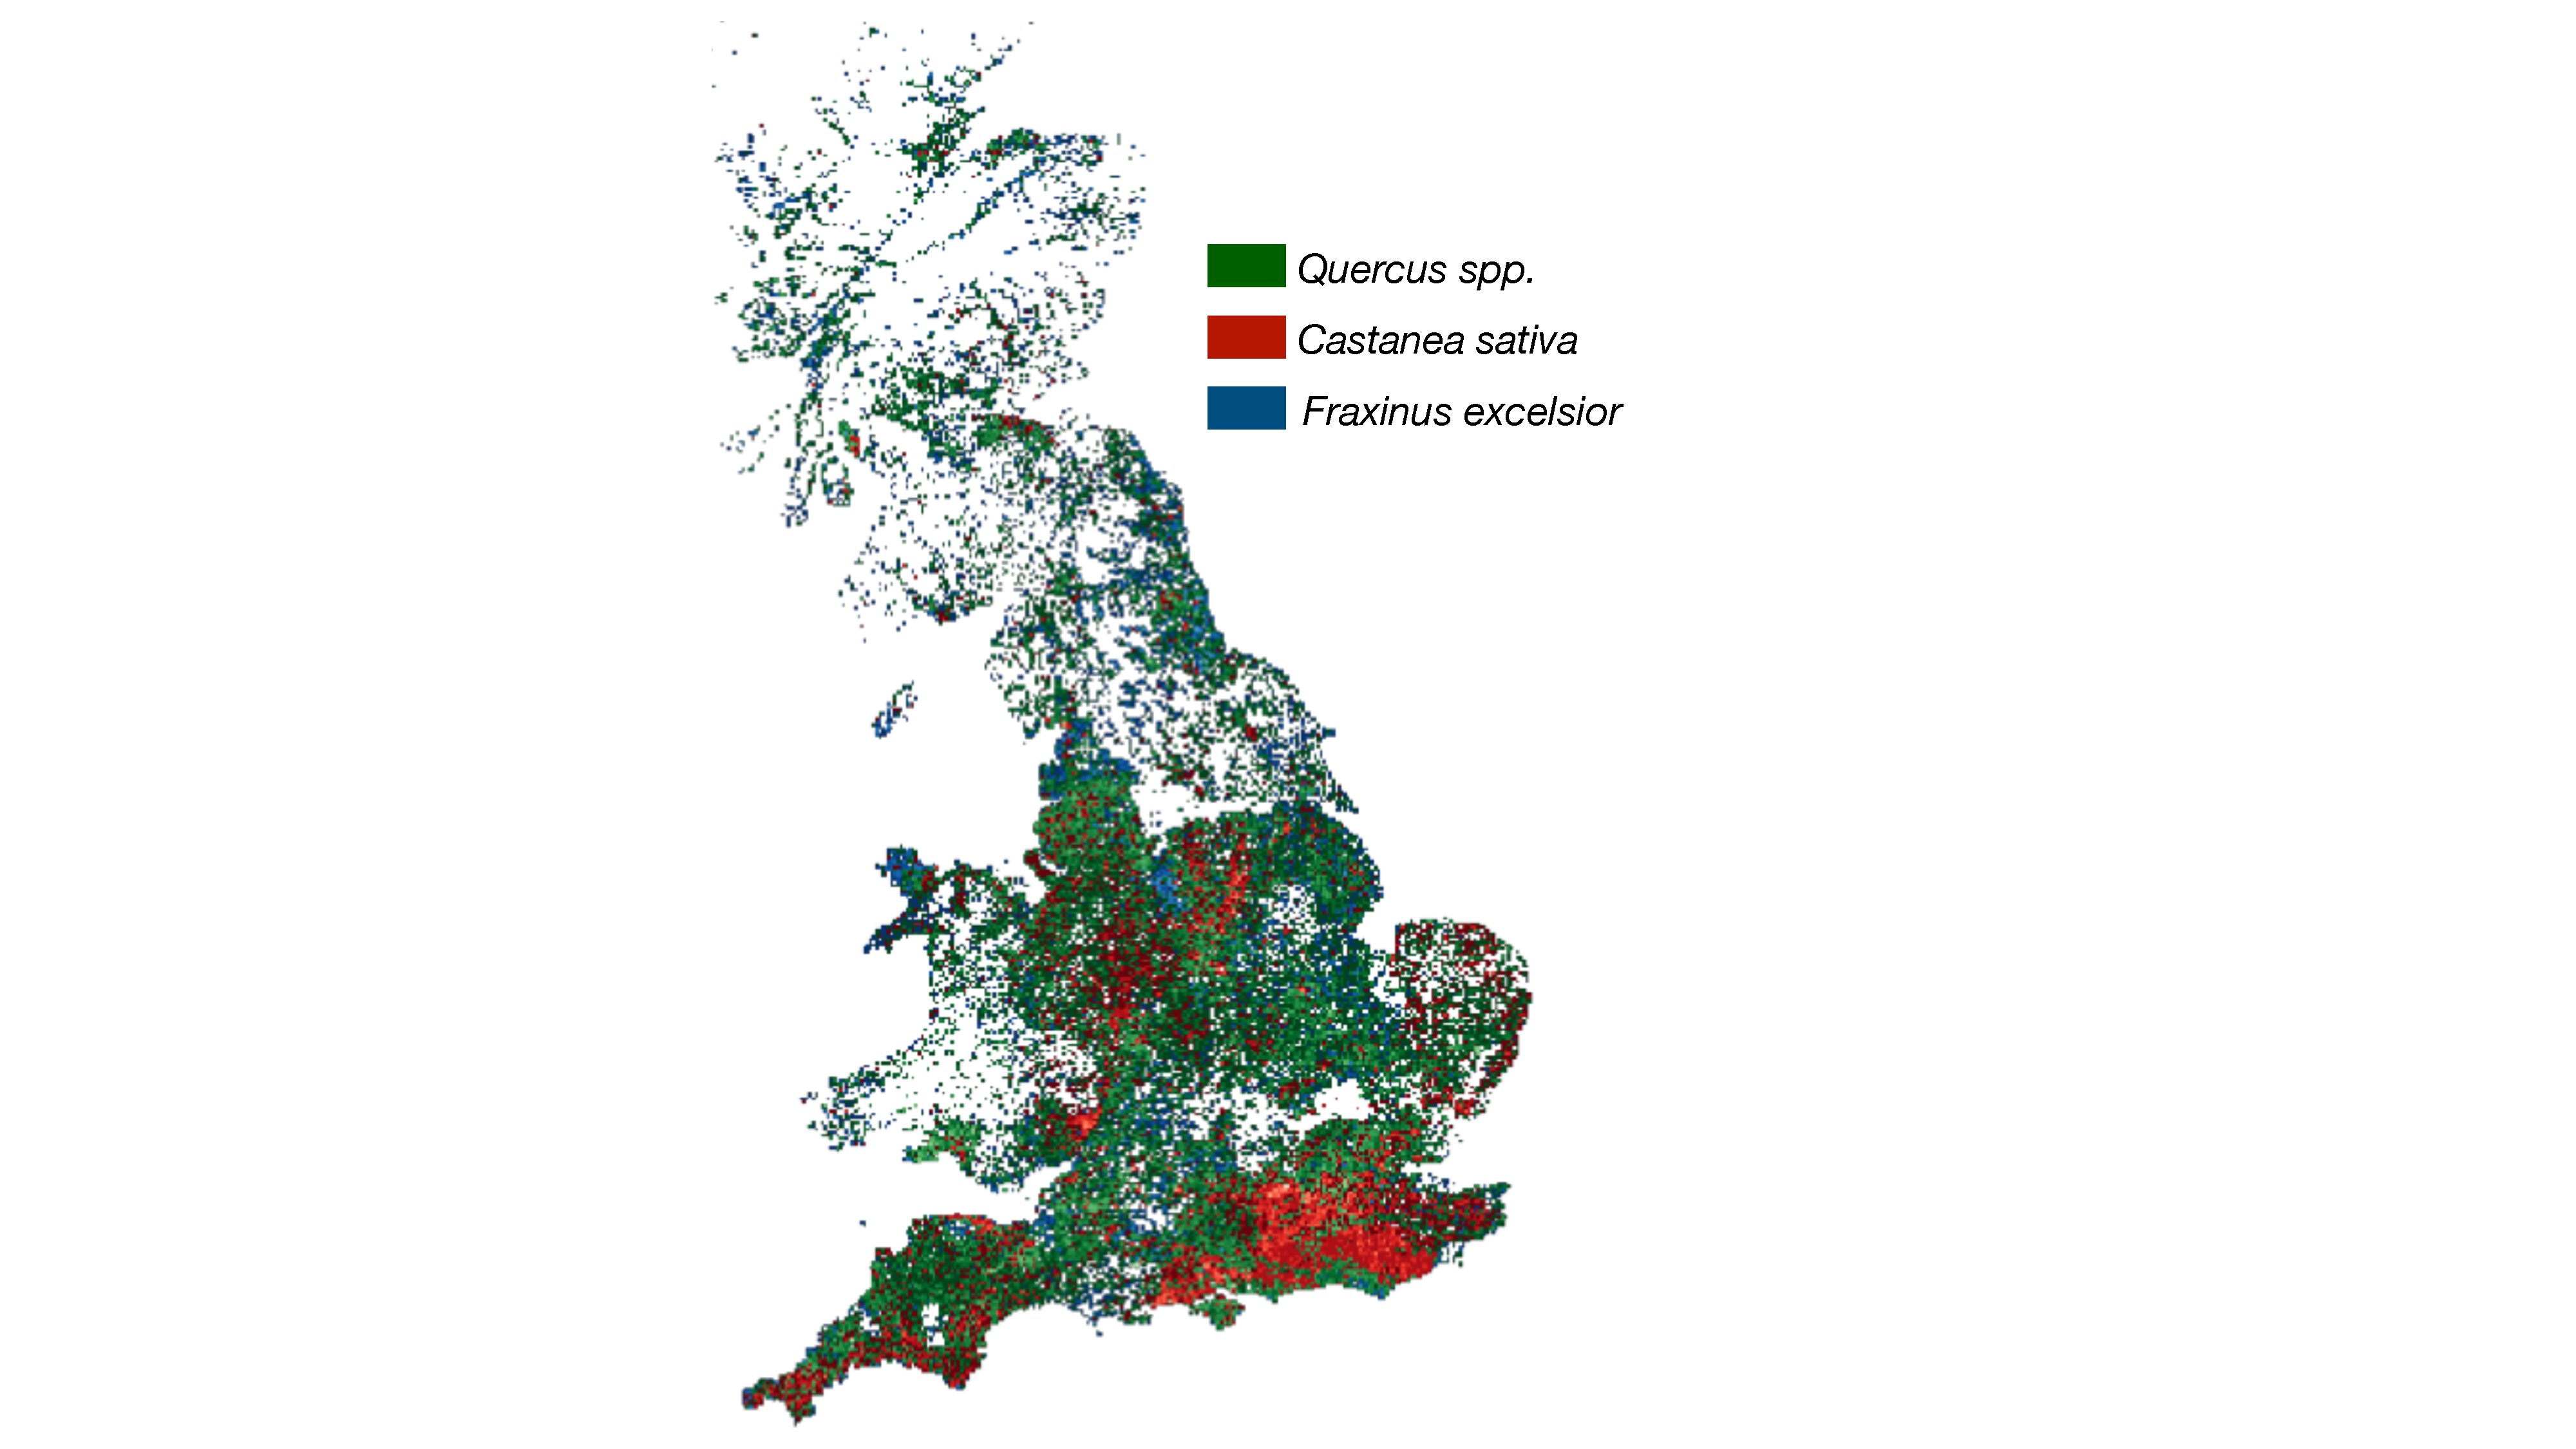
\includegraphics[scale=0.25]{chapter2/figures/bsbi-data.pdf}
    \caption{BSBI presence-only datasets\textemdash as reconstructed by S. Orozco-Fuentes et al. (unpublished).
    Three important large deciduous tree species, European ash (\textit{Fraxinus excelsior}), 
    Oak (\textit{Quercus spp.}), and sweet chestnut (Castanea sativa), are overlaid onto the same map at $\mathrm{2km \times 2km}$ resolution.
    The BSBI datasets are extensive and report presence-only data over a country-wide scale.
    }
    \label{fig:bsbi-data}
\end{figure}

The Botanical Society of Britain and Ireland (BSBI) has recorded species presence-only data since $1950$.
BSBI datasets are publicly available\footnote{BSBI data can be downloaded from: \nolinkurl{https://database.bsbi.org}.} upto a
resolution of $\mathrm{2 km \times 2km}$, though records upto $\mathrm{100 m \times 100 m}$ are available to registered members.
As of $2020$, BSBI records are collected at $\mathrm{1 km \times 1km}$ square resolution or better\textemdash making the datasets among the 
highest-resolution surveys collected by traditional methods. The BSBI distribution database contains records of plants and charophytes
as reported by users and conservationists with MapMate\footnote{MapMate is software designed to aid users to share ecological data: \nolinkurl{https://www.mapmate.co.uk}}.
Despite the availability of high-resolution data, observations are collected ad hoc by users and not curated scientifically.
Moreover, the distributions contain both well-surveyed and poorly-surveyed plots of land likely to carry uncertainties.
As such, BSIBI data is helpful to reconstruct several baseline tree distributions across GB, as demonstrated by \cite{hill.data}.

\subsection{Species distribution models}

\begin{figure}
    \centering
    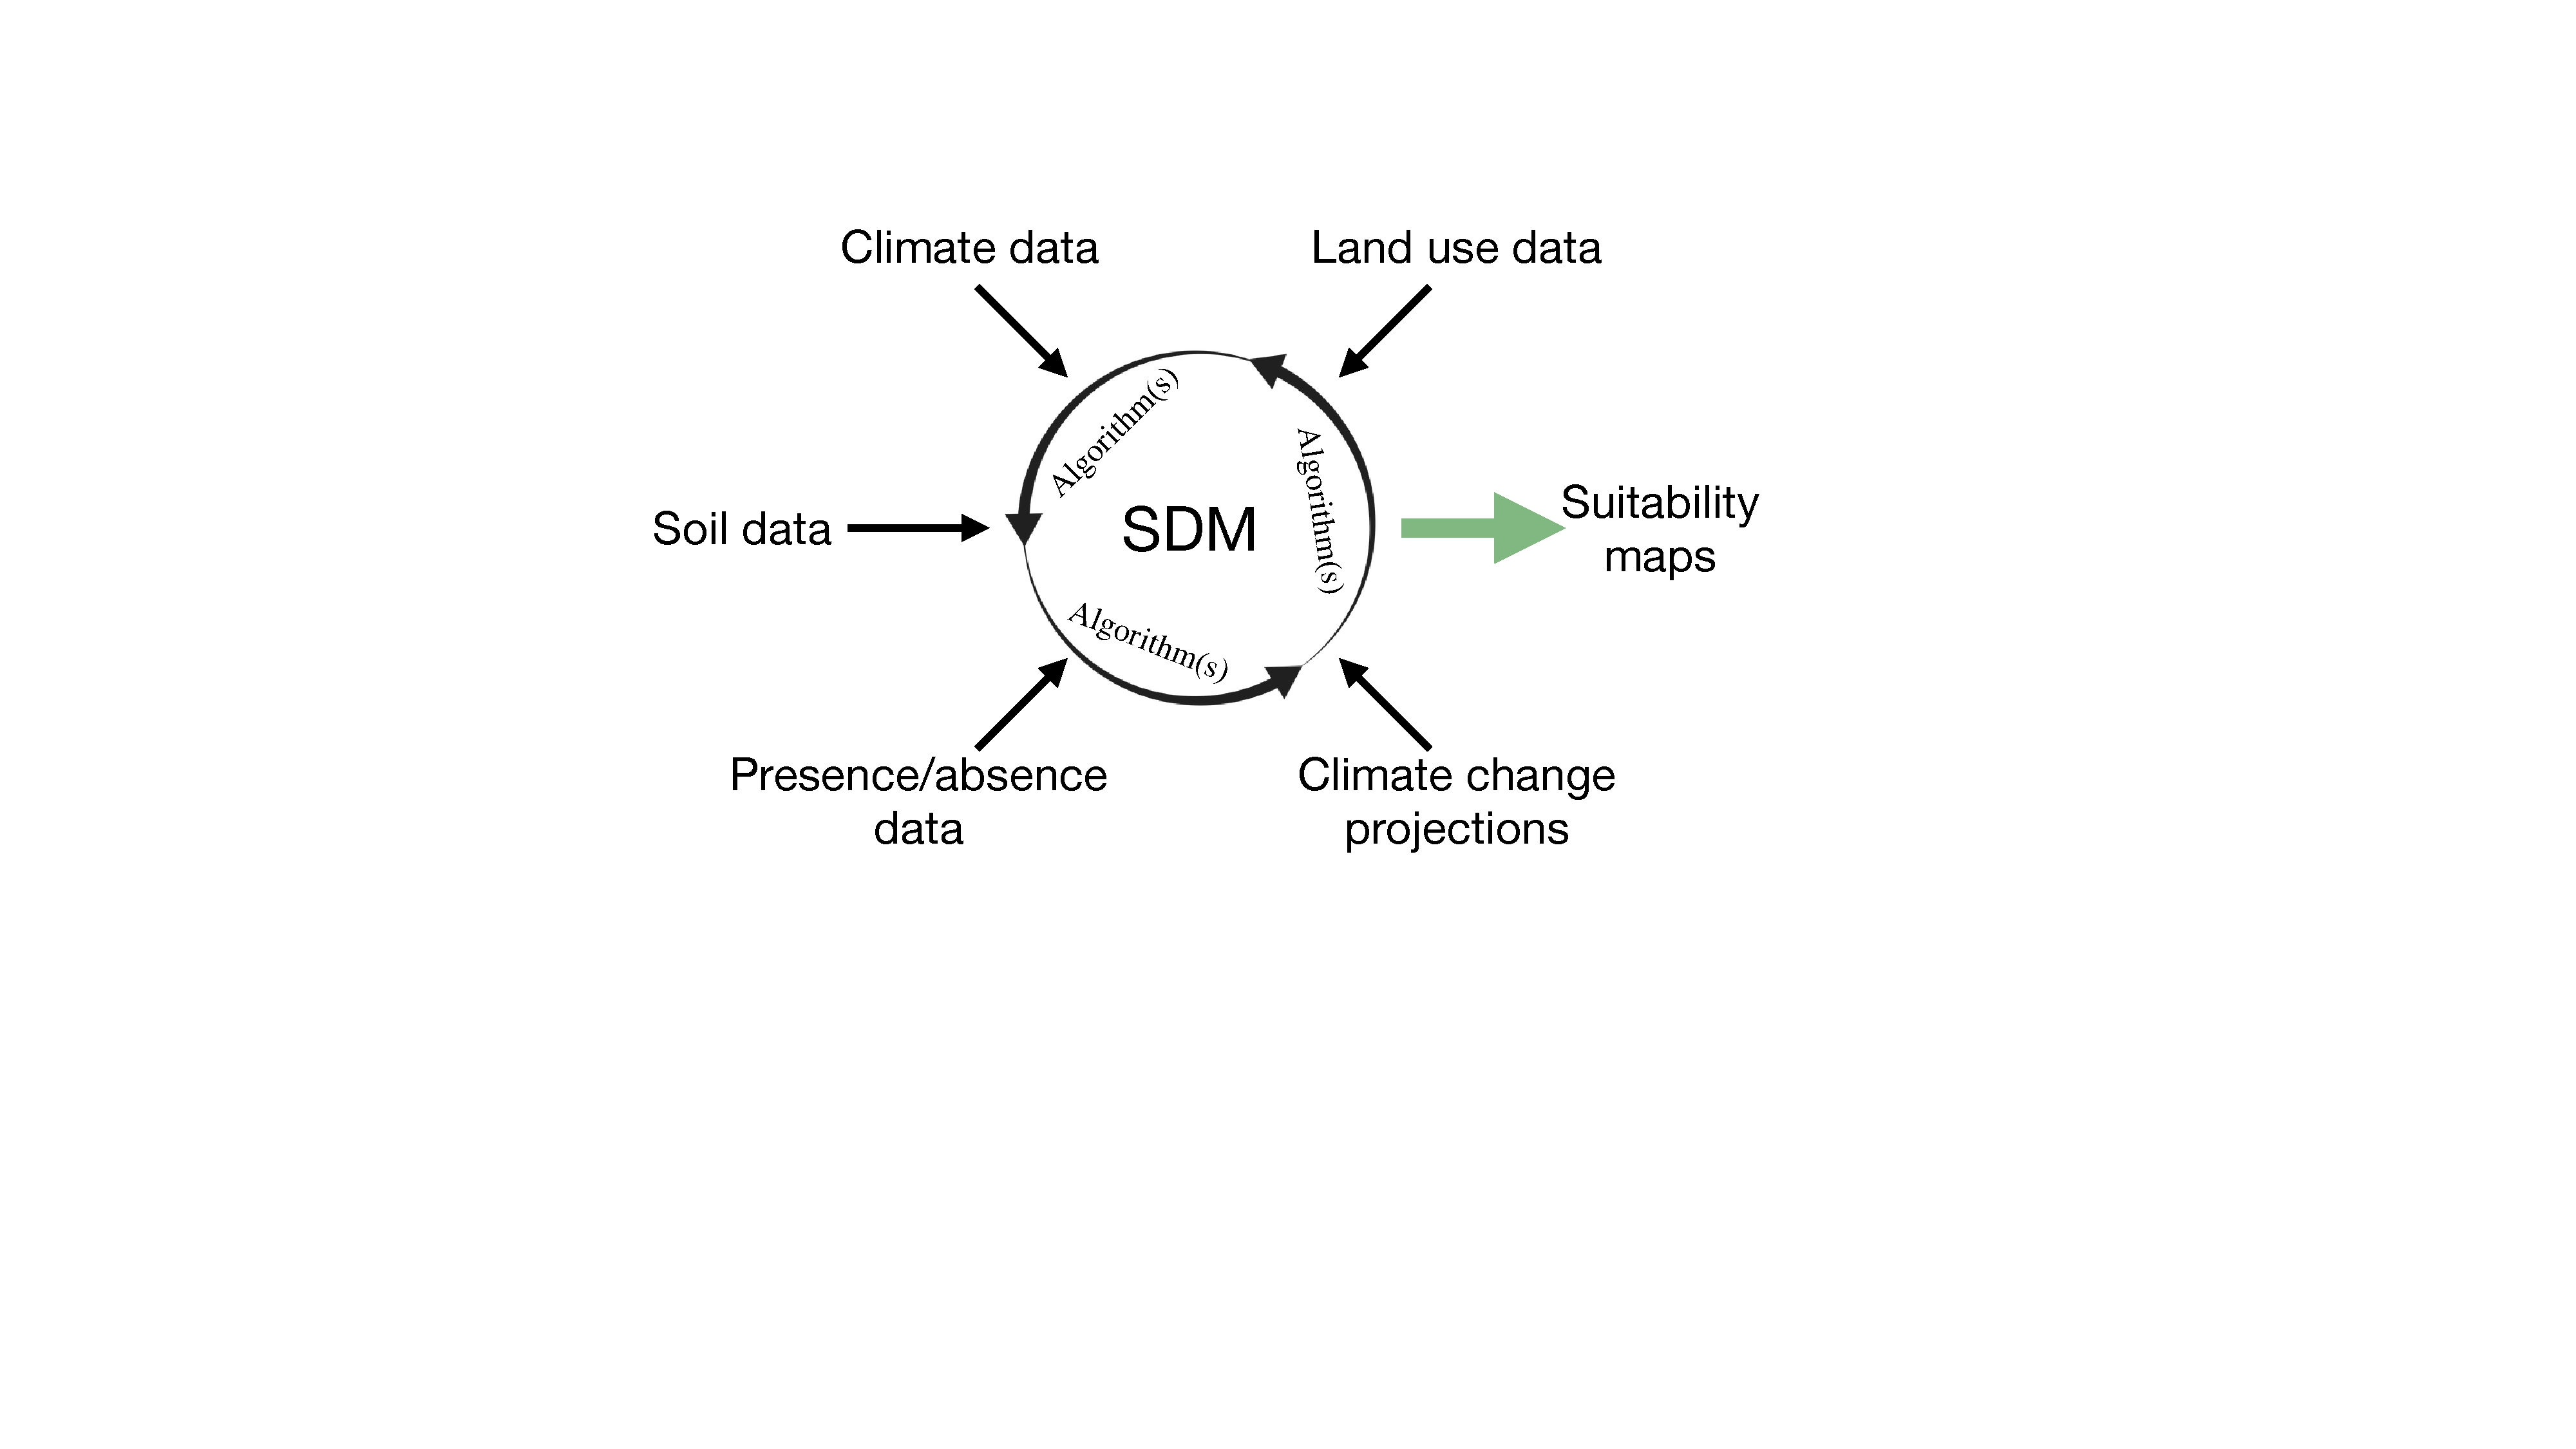
\includegraphics[scale=0.35]{chapter2/figures/SDM-fig.pdf}
    \caption{A graphical species distribution model (SDM) illustration, adapted from \cite{SDM_1}. 
             A variety of predictor variables and input data sources are used in conjugation with modelling algorithms to produce
             a habitat suitability map.}
    \label{fig:sdm}
\end{figure}

Species distribution models (SDMs) aim to generate data, from less-extensive surveyed data.
SDMs were first developed in the $1990$s, and have subsequently become fundamental to ecological and biogeographical inference studies.
Inferred, or modelled, species distribution data have been used to examine biodiversity, conservation, resource management, 
ecology and climate change \cite{austin2011improving, franklin2013species, skov2016real, wittmann2016confronting, 10.3958/059.037.0110, zhang2019using}.
The vast majority of SDMs fall into two categories: correlative \cite{srivastava2019species}, and mechanistic \cite{shabani2016comparison}.

Correlative SDMs relate (widely available) presence-only, or presence-absence, data to several environmental predictor variable datasets.
For tree species, predictor variables include temperature, precipitation, altitude, and soil type \cite{ray2021multi, hill.data}.
Following this, a species distribution map can be predicted, albeit with  uncertainties and errors.
Commonly used statistical methods include Regression 
(i.e. General Linear Models, General Additive Models, Multivariate Adaptive Regression Splines) and Machine Learning
(i.e. Artificial Neural Networks, Classification And Regression Tree, Random Forest). 
The general correlative approach is reflected in Figure \ref{fig:sdm}; for a more in-depth review of correlative SDMs, see \cite{SDM_1}.

Correlative SDM approaches require little to no prior knowledge of the physiological processes that link organism and environment.
Hence, mechanistic methods aim to incorporate an organisms behavioural, physiological, and morphological constraints to the environment, 
as reviewed by \cite{kearney2009mechanistic}. However, linking a species physiological response to the environment comes with significant
computational challenges, as it typically relies on vast, multi-variable time-series datasets \cite{shabani2016comparison}.

A review paper by \cite{guillera2015my}, revealed a diverse use of SDMs.
Out of $100$ publications reviewed by \cite{guillera2015my}, SDMs were applied to: 
1) managing threatened species ($16\% $ of articles) 
2) predicting climate change impacts ($13\%$) 
3) understanding phylogeographic patterns ($9\%$) 
4) controlling threatening processes ($8\%$) 
5) landscape management ($8\%$) 
6) biological invasions ($7\%$). However, no epidemic applications were reported.

Nevertheless, a thorough literature search revealed a variety of epidemiological SDM applications.
The crossover between ecological SDM methods and epidemiology has been referred to as `Infectious Disease Cartography' \cite{KRAEMER201619}.
With Infectious Disease Cartography, one seeks to map the likelihood, or risk, of infectious disease outbreaks and produce risk-maps.
A number of publications have applied SDMs livestock diseases \cite{hollings2017species}, and human-based diseases including the global 
distribution of Dengue Fervour \cite{bhatt2013global} and Zika virus \cite{messina2016mapping}, and Anthrax in Kenya \cite{otieno2021modeling}.
However, SDM applications for tree disease epidemics appear absent from the literature.

\subsubsection{Modelling tree abundance}

SDM-generated tree occurrence data has limited applications to ecologists and forest managers.
This motivates a statistically-generated abundance data, that includes significantly 
more information about the population occupation/density and ecosystem.
Modellers have examined numerous approaches to predict species abundance;
including, linking the abundance-occupancy relationship \cite{gaston2000abundance} and
the scaling pattern of species occupancy over progressively smaller spatial scales \cite{hui2009extrapolating}.

An interesting, and highly relevant, approach to predict the abundance of common tree species in Great Britain was put forward by \cite{hill.data}.
At a high level, (BSBI) presence-only data was combined with a series of environmental covariates using a species distribution model to 
produce a map of predicted occurrence data. Then, random forest regression was employed with a training sample ($70\%$) of less extensive abundance 
data\textemdash consisting of Countryside survey, myForest and Bluesky's National Canopy Map. 
Results were then cross-validated with the remaining ($30\%$) abundance data; Figure \ref{fig:hill-method} displays a
flow-diagram of the method presented by \cite{hill.data}. 

A more detailed explanation of the treatment proposed by \cite{hill.data} follows:
\textbf{Stage 1)}
\textit{
\begin{itemize}
    \item Presence-only BSBI data was downloaded for $25$ common species of trees in GB, 
    and all records less than $\mathrm{2km \times 2km}$ resolution were discarded.
    Next, the presence-only data was converted into presence-absence data by considering
    `well-surveyed' records that Hill et.al defined as having a minimum of two survey
    between $1950$ and consisting of $50$ species. Species missing from these 
    well-surveyed areas were assumed truly absent. 
    \item Using biomod2 \cite{thuiller2016package}, a SDM was then fitted against a cohort of 15 environmental variables, e.g.
    soil type (European Soil Database), temperature (Worldclim), precipitation (Worldclim), altitude (Worldclim),
    type of land cover (Countryside Survey), among others. The net result was a map of predicted occupancy at $\mathrm{1 km \times 1 km}$ 
    resolution.
    \item For each species, predictions from a suit of models\textemdash GLM, GAM, CTA, GBM, RF\textemdash were
    repeated and combined into an ensemble distribution model. Each model was cross-validated against
    $30\%$ of the well-survyed BSBI presence-absence data using the receiver operator curve (ROC) and the true skill statistic (TSS).
    \cite{hill.data} then selected the best performing predicted occurrence for each species.
\end{itemize}
}
\textbf{Stage 2)}
\textit{
\begin{itemize}
    \item Abundance data from Countryside survey (CS) and myForest were both expressed as hectares covered per kilometer 
    squared ($\mathrm{ha/km^2}$). This entailed using woodland cover data from the National Forest Inventory (NFI) to multiply
    the percentage cover of each species within a woodland patch, with a proportion of woodland cover per kilometer.
    \item Random forest (RF) regression then modelled the relationships between (CS and myForest) abundance data with
    the SDM-generated map of predicted occupancy. In addition, RF regression used four covariates, 
    three of which consisted of Bluesky's National Canopy data (i.e. total tree cover, woodland tree cover, non-woodland tree cover)
    and NFI edge broadleaved woodland (i.e. within $50\mathrm{m}$ of non woodland) data.
\end{itemize}
}

The abundance datasets produced by \cite{hill.data} combine several mainstream tree datasets in GB; moreover, 
constructing the ensemble model involved a variety of statistical models.
The predicted occurrence data was examined against the Receiver operating characteristic (ROC) \cite{jimenez2012insights}.
Most species demonstrated functional ROC scores between $0.71$ and $0.96$ and performed exceptionally
well for ash ($0.96$) and oak ($0.90$).  

Although, numerous assumptions underpinned the method of predicting occupancy.
Primarily, the BSBI dataset used by \cite{hill.data} exists through ad-hoc user and volunteer self-reports.
Thus, some regions are more surveyed than others over the years, this led Hill et al. to make the 
`well surveyed' recorded assumption (i.e. only considering records surveyed twice since $1950$ containing a minimum of $50$ species).
The assumption permitted the conversion of raw presence-only to presence-absence, 
at the cost of overestimated absence in these regions. That is, even supposing $50$ species
are reported within a subset of the ($\mathrm{2km \times 2km}$ tetrad) record, other large regions could remain unsampled. 
We remark the authors did not appear to scrutinise this assumption sufficiently.

\begin{figure}
    \centering
    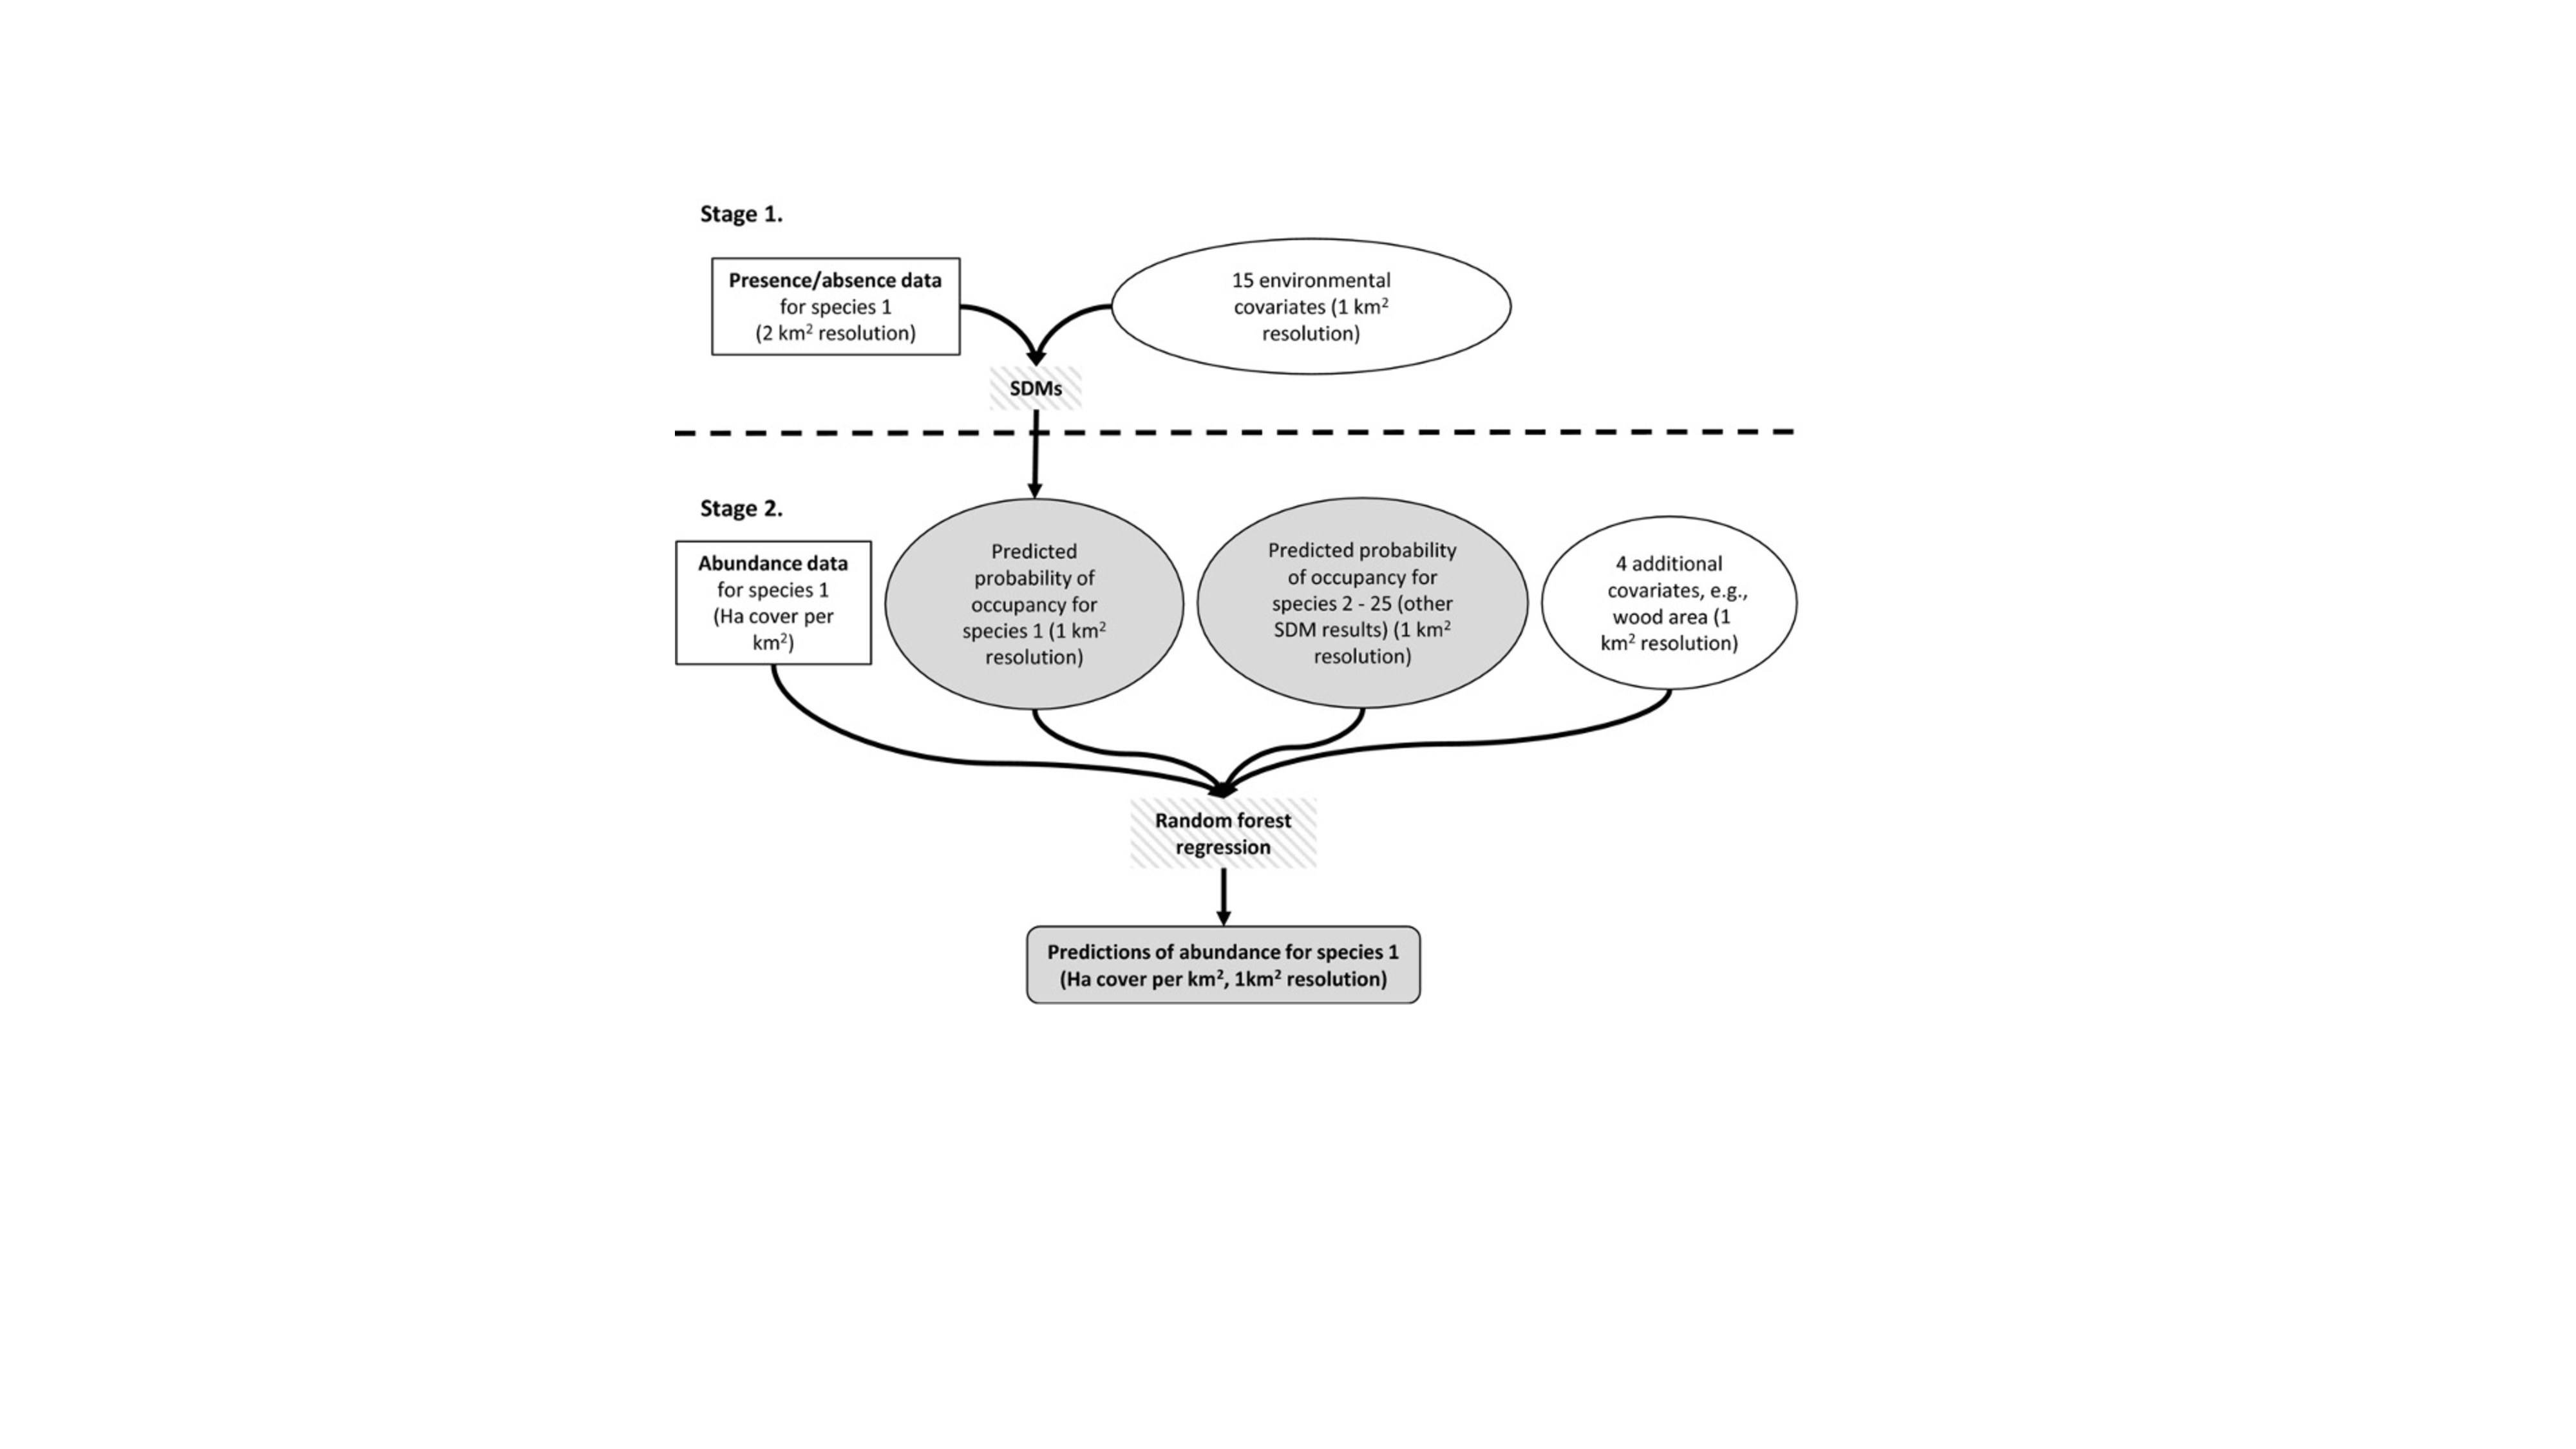
\includegraphics[scale=0.55]{chapter2/figures/hill-method-fig.pdf}
    \caption{A flow diagram of the two-stage abundance method put forward by \cite{hill.data} to model tree species abundance  
    (taken from the publications' materials and methods section).}
    \label{fig:hill-method}
\end{figure}

The RF regression used by \cite{hill.data} marked a novel approach to modelling species abundance.
The authors chose to argue in favour of RF regression because of its insensitivity toward the data distribution,
which worked well with the less comprehensive abundance data sources (as the map of abundance had a high percentage of zeros from missing records).
The abundance model quality was examined against $10$-fold validation (explained in \cite{refaeilzadeh2009cross}).
The root-mean-square error (RMSE), between predicted and observed abundance, generally ranged between $5$ and $10$,
where the RMSE scale reflects the response variable units ($\mathrm{ha/km^2}$), i.e. $5\%$ and $10\%$ respectively.
The result was country-wide predicted abundance.

The low amount of available abundance data in GB significantly impoverished the abundance maps produced by \cite{hill.data}. 
Consequently, datasets for the $25$ species considered will contain numerous (small-scale) errors and uncertainties. 
Nonetheless, the modelled abundance maps captured more large-scale spatial structures than the original BSBI and CS distributions.
More recently, \cite{ray2021multi} produced a similar SDM as Hill et al. for oak in GB using biomod2 \cite{thuiller2016package}.
The authors focused on mapping high-density oak woodlands (with 60$\%$ canopy cover or above) 
to predict which NFI map polygons (by forest type) were most likely to contain oak stands. 
However, \cite{ray2021multi} did not make their oak maps publicly available, nor did they produce a general-purpose
abundance map relevant for epidemiological studies. 
To date, the predicted abundance maps produced by \cite{hill.data} constitute the best publicly available 
country-wide maps in GB, despite their limitations.

%\item remote sensing tools were used \cite{kelly2002monitoring} to track the study of sudden oak death in California
%\item \cite{kelly2002landscape} demonstrated clustering at the landscape level, spatial structure is important

\section{Ash dieback case study}

% - the combination of ash dieback and emerald ash borer present a significant threat to UK and European ash \cite{musolin2017between}
% - managing the spread of ADB in areas already infected is hardly possible \cite{gross2014h}
% - but slowing the spread of disease is still valuable to allow ash populations vital time to recover and policy makers \cite{PAUTASSO201337}
% - multi-scale approaches have been outlined \cite{hart2020theoretical}

\label{ch2:ash-dieback}
Ash dieback (ADB) presents an interesting case study of an emerging epidemic currently devastating ash
populations throughout Europe \cite{enderle2019overview}. The history and predicted evolution of ash dieback
demonstrate how an invasive, non-indigenous pathogen can spread rapidly through a foreign ecosystem that 
lacks evolutionary defences. Among the many factors driving the spread of ash dieback, long-distance 
anthropomorphic trade is the mechanism responsible for the initial introduction into Europe from the
far-east \cite{zhao2013hymenoscyphus, queloz2011cryptic}.

The pathosystem has been the subject of much research over the years. As a result, the taxonomy, 
symptoms and life-cycle of the pathogen are  now well-known \cite{https://doi.org/10.1111/mpp.12073}. 
Understanding the spread of ADB and managing the epidemic impact on ecosystems could only be achieved
by the confluence of molecular biologists, forest managers, policymakers and modellers. Although the epidemic
is well underway, slowing the spread of ash dieback remains essential to allow ash populations time to adapt.

\subsection{Historical developments}

Reports of dieback on ash began surfacing in Poland in $1992$, but a causal agent was not established
for a decade \cite{kowalski2001zamieraniu, coetsee2000xenochalara}. Subsequently, \cite{kowalski2006chalara} 
recognised a novel pathogenic fungus to be the causal agent, identified as an ascomycete anamorph (i.e. an asexual fungus).
The fungus was named \textit{Chalara fraxinea}, a member of the hyphomycete genus \textit{Chalara}. 
The sexual teleomorphic stage of the pathogen was later attributed to \textit{Hymenoscyphus albidus} 
\cite{kowalski2009teleomorph}, a well-known non-pathogenic fungus indigenous to Europe.

Linking the hitherto non-pathogenic \textit{H. albidus} to the agent causing ash dieback perplexed researchers. 
The enigma was resolved through DNA sequencing by \cite{queloz2011cryptic} when a second morphologically identical
ascomycete named \textit{`Hymenoscyphus pseudoalbidus'} was identified as the pathogen responsible for widespread dieback
of European ash in a process referred to as `Cryptic speciation'.

Interestingly, the emergent epidemic caused by \textit{H. pseudoalbidus} coincided with developments 
in the phylogenetic classification system of the kingdom Fungi \cite{hibbett2007higher}, 
and dual nomenclature\footnote{Originally, fungi were classified through the structure of their sexual organs.
Problematically, ascomycete fungi have a complicated dual reproductive mode (both sexual and asexual) that often caused confused. 
However, a move toward a one-name fungi classification system has since simplified fungi taxonomy.} 
\cite{wingfield2012one}. Subsequently, the pathogen \textit{`Hymenoscyphus pseudoalbidus'} was renamed to
\textit{Hymenoscyphus fraxineus} (HF).

\subsection{Symptoms and epidemiology}

European ash is highly susceptible to HF because it has no (co-evolved) evolutionary defence.
Although HF is lethal to European ash, it poses little threat to its native Asian hosts 
\textit{Fraxinus mandshurica} and \textit{Fraxinus chinensis}. Once the fungus colonises a European ash leaf,
it can spread through twigs, branches, the xylem, and eventually the whole tree.
The symptoms include necrotic lesions, crown dieback, wilting and eventual death.
In addition to leaf-infections, the pathogen can colonise the root-system \cite{schumacher2011general}.
Root-infections usually occur in already severely infected ash \cite{https://doi.org/10.1111/mpp.12073}. 
After which, it is only a matter of time before opportunistic fungi invade and significantly accelerate mortality
\cite{enderle2013temporal}.

The progressive symptoms of ADB, as presented by \cite{gross2014h}, are displayed in Figure \ref{fig:ash-deiback-symptoms}.
Ascospores initially infect susceptible ash leaves (a), 
becoming visible after around two weeks \cite{https://doi.org/10.1111/ppa.12048} in the summertime. 
In Figure \ref{fig:ash-deiback-symptoms}, panels (b-d) show the initial infection spreading through 
the leaf into the rachis and the development of the first necrotic lesions\textemdash see
\cite{https://doi.org/10.1111/ppa.12844} for further information on the precise mechanism of ascospore leaf penetration.

Over winter, the infection continues to spread through ash. 
Young ash develop large visible necrotic lesions, as illustrated in Figure \ref{fig:ash-deiback-symptoms}(e-i).
In spring, the infection causes shoot wilting (g) and death (h-i) before causing xylem necrosis (j).
Over many seasons, large infected mature ash trees begin to die (l) as it begins forming epicormic branches, 
as noted by \cite{marciulyniene2017can} and losing its canopy.

\begin{figure}
    \centering
    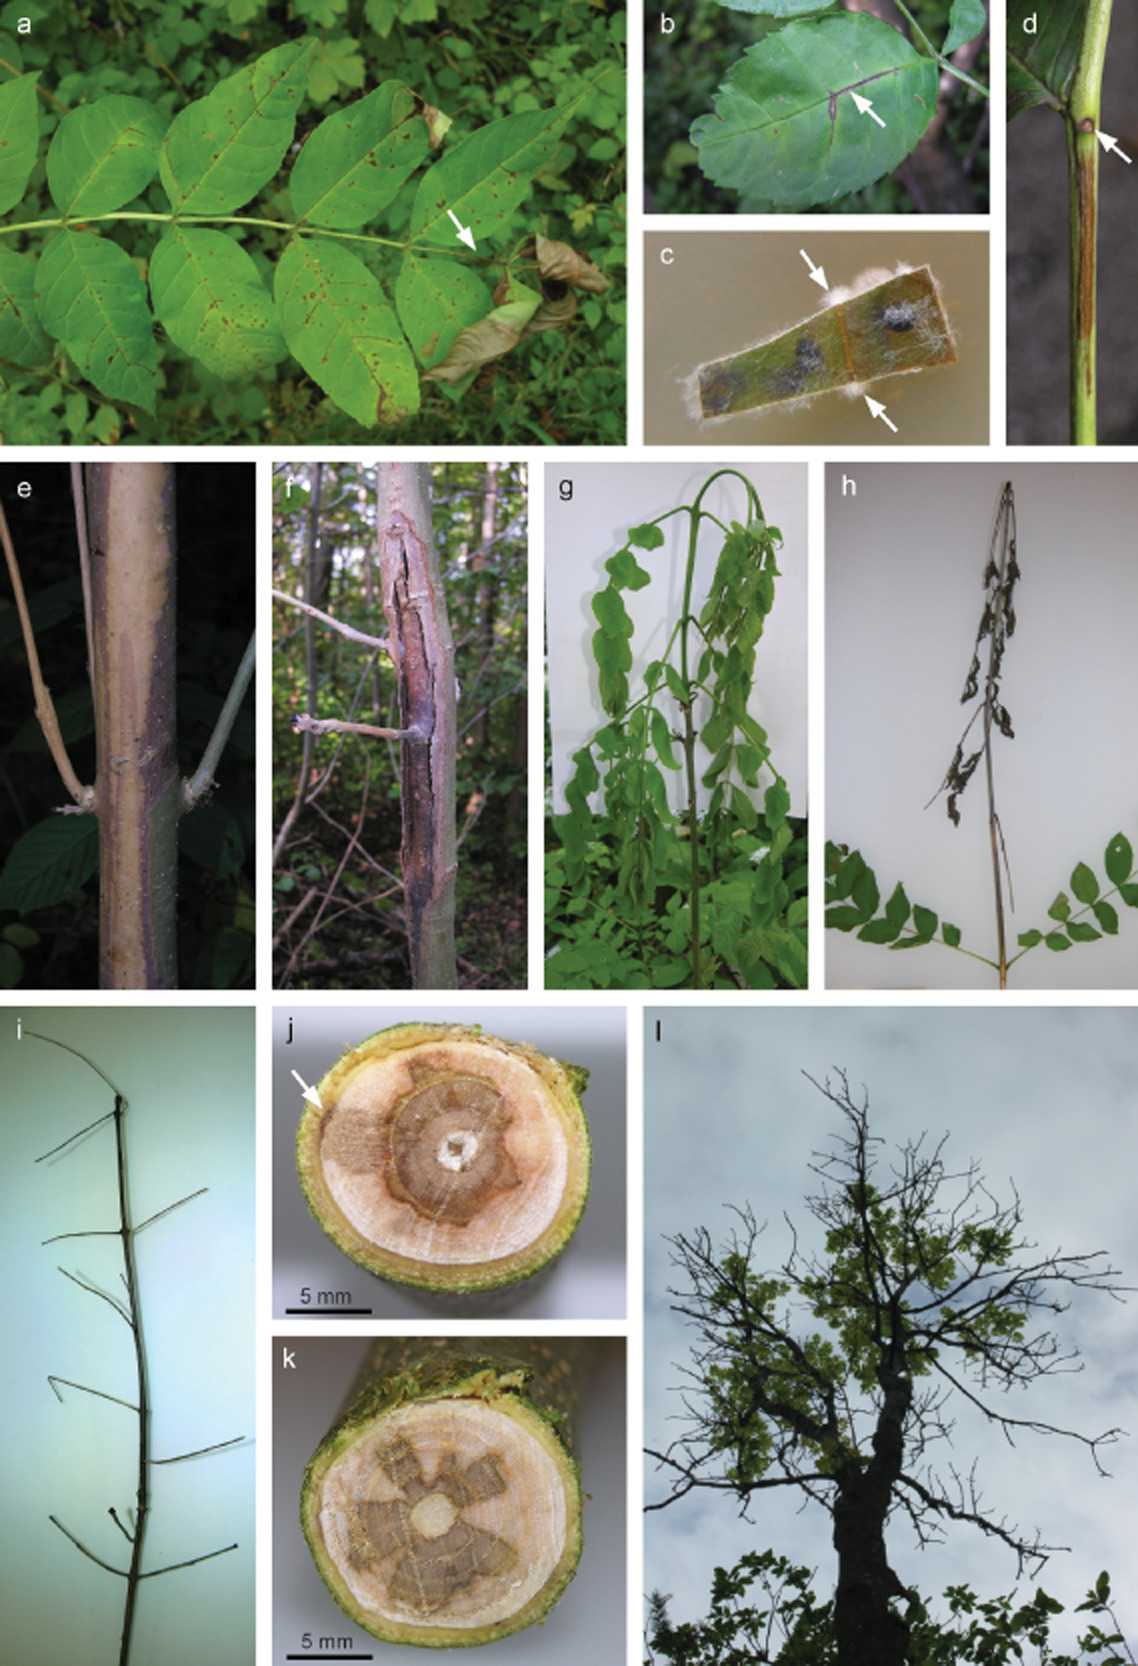
\includegraphics[scale=0.5]{chapter2/figures/gross2014.jpg}
    \caption{
    The symptoms of ash dieback, taken from the work of \cite{gross2014h}. 
    The pathogen \textit{H. fraxineus} infects the leaves of ash, leading to early onset wilting and desiccation. 
    The fungus then reproduces asexually, spreading through twigs, branches and eventually the xylem. 
    Symptoms include wilting, necrotic lesions, crown dieback and eventual mortality.}
    \label{fig:ash-deiback-symptoms}
\end{figure}

The pathogen HF is lethal to European ash (\textit{Fraxinus excelsior}) of all ages. 
Nevertheless, research has established that small young ash trees are more at risk,
and susceptibility declines with maturity. Surveys of ash stands conducted by \cite{marccais2017estimation} 
in Belgium recorded that after six years of infection, small young saplings died with $35\%$ mortality, 
whilst slightly larger ash ($<25 \mathrm{cm}$ in diameter) displayed mortality of $11\%$. 
In contrast only $3.2\%$ of large mature ash ($>25\mathrm{cm}$ in diameter) died.

Various sources of ash mortality data have been collected in different European countries;
in Germany, a forest stand of planted ash trees showed a $73\%$
mortality rate after five years \cite{langer2015ash} (as cited in a review
\cite{enderle2017ash}), while observations of ADB progression in Austria
suggest a low mortality rate of $5\%$ measured over a two-year window \cite{kessler2012dieback}. 
A study conducted at different sites throughout Great Britain suggests a time scale ranging between 
$3-15$ years of infected tree growth before death \cite{wylder2018evidence}.

In addition to age, ash survival also depends on the landscape. 
Landscape features and ADB progression were studied by \cite{https://doi.org/10.1111/1365-2745.13383} 
over a sample plot of size  $\mathrm{3.5km \times 6.5 km}$ in France; observations over two years
suggest that the surrounding landscape has little impact initially in $2012$. However, after pathogen establishment, 
later surveys in $2016$-$2018$ showed that landscape features play an essential role.
Among the results put forward by \cite{https://doi.org/10.1111/1365-2745.13383}, 
a highly abundant ash region increased the prevalence of collar canker and rachis symptoms in neighbouring ash.
In addition, the authors found that the influence of ADB decayed exponentially up to $200-300\mathrm{m}$ away from the high density source,
thus suggesting a density-dependency in ADB spread.

Modelling work suggests a myriad of environmental factors can also predict the
vulnerability of ash and subsequent spread of disease \cite{dal2014risk}.
Spatial regression analysis conducted by \cite{chumanova2019predicting} in the Czech Republic indicates that altitude 
is an important predictor of pathogen growth, which also support the strong negative temperature dependence observed by \cite{hauptman2013temperature}.

\subsection{Life cycle and reproductive mode}
% WIKI: Hymenoscyphus fraxineus has two phases to its life-cycle: sexual and asexual.[9] The asexual stage (anamorph) grows in affected trees attacking the bark and encircling twigs and branches.[9] The sexual, reproductive stage, (teleomorph) grows during summer on ash petioles in the previous year's fallen leaves.[7] The ascospores are produced in asci and are transmitted by wind; this might explain the rapid spread of the fungus.[

The reproductive mode is intricate, and HF can infect hosts through the soil,
water, and air \cite{gross2012reproductive}; 
although, the primary natural driver of disease propagation is through wind-dispersal
during summertime sporulation. Sporulation typically occurs from June-September when 
fungal fruiting bodies on the previous litter-fall release ascospores \cite{grosdidier2018tracking, hietala2013invasive}.
Multiple ascospores sources can infect the same leaf \cite{gross2012reproductive}. 
Though the primary natural driver is wind, infection (and re-infection) of ash are also thought to be possible 
through the soil-borne mechanisms \cite{fones2016role}, albeit with low frequency.

Ash dieback is highly seasonal \cite{bengtsson2014seasonal} and follows a complex, yearly polycyclic infection cycle.
Infected ash hosts will shed their leaves in the autumn, proceeded by fungal fruiting bodies growing on the dead leaf litter until summertime.
In summer, fruiting body spores are wind-dispersed and continue the cycle by producing new secondary infections\textemdash 
together, the life cycle and symptom expressions are illustrated in Figure \ref{fig:ash-deiback-symptoms}.
It is interesting to note the cyclic similarities between yearly ADB infection/re-infection and the seasonal
infections due to crop rotations, e.g. \cite{tankam2020modelling}. 
Notwithstanding that infected crop removal usually coincides with harvest time instead of infected ash survival that can span years.

The life cycle of the fungus HF can be understood to have two well-differentiated reproductive modes, 
sexual and asexual\textemdash a common trait of phyla Ascomycota, or ascomycetes fungi \cite{hawker2016physiology}.
Initially, asexual spores (conidia) were hypothesised to only increase genetic variance and act as spermatia \cite{gross2014h};
however \cite{fones2016role} called this into question, suggesting instead that asexual reproduction of the pathogen 
may play a role in driving the pathogen spread. Despite the potentially significant claim put forward by \cite{fones2016role},
it has gained seemingly little traction, and the role of asexual reproduction is still not fully understood.

\begin{figure}
    \centering
    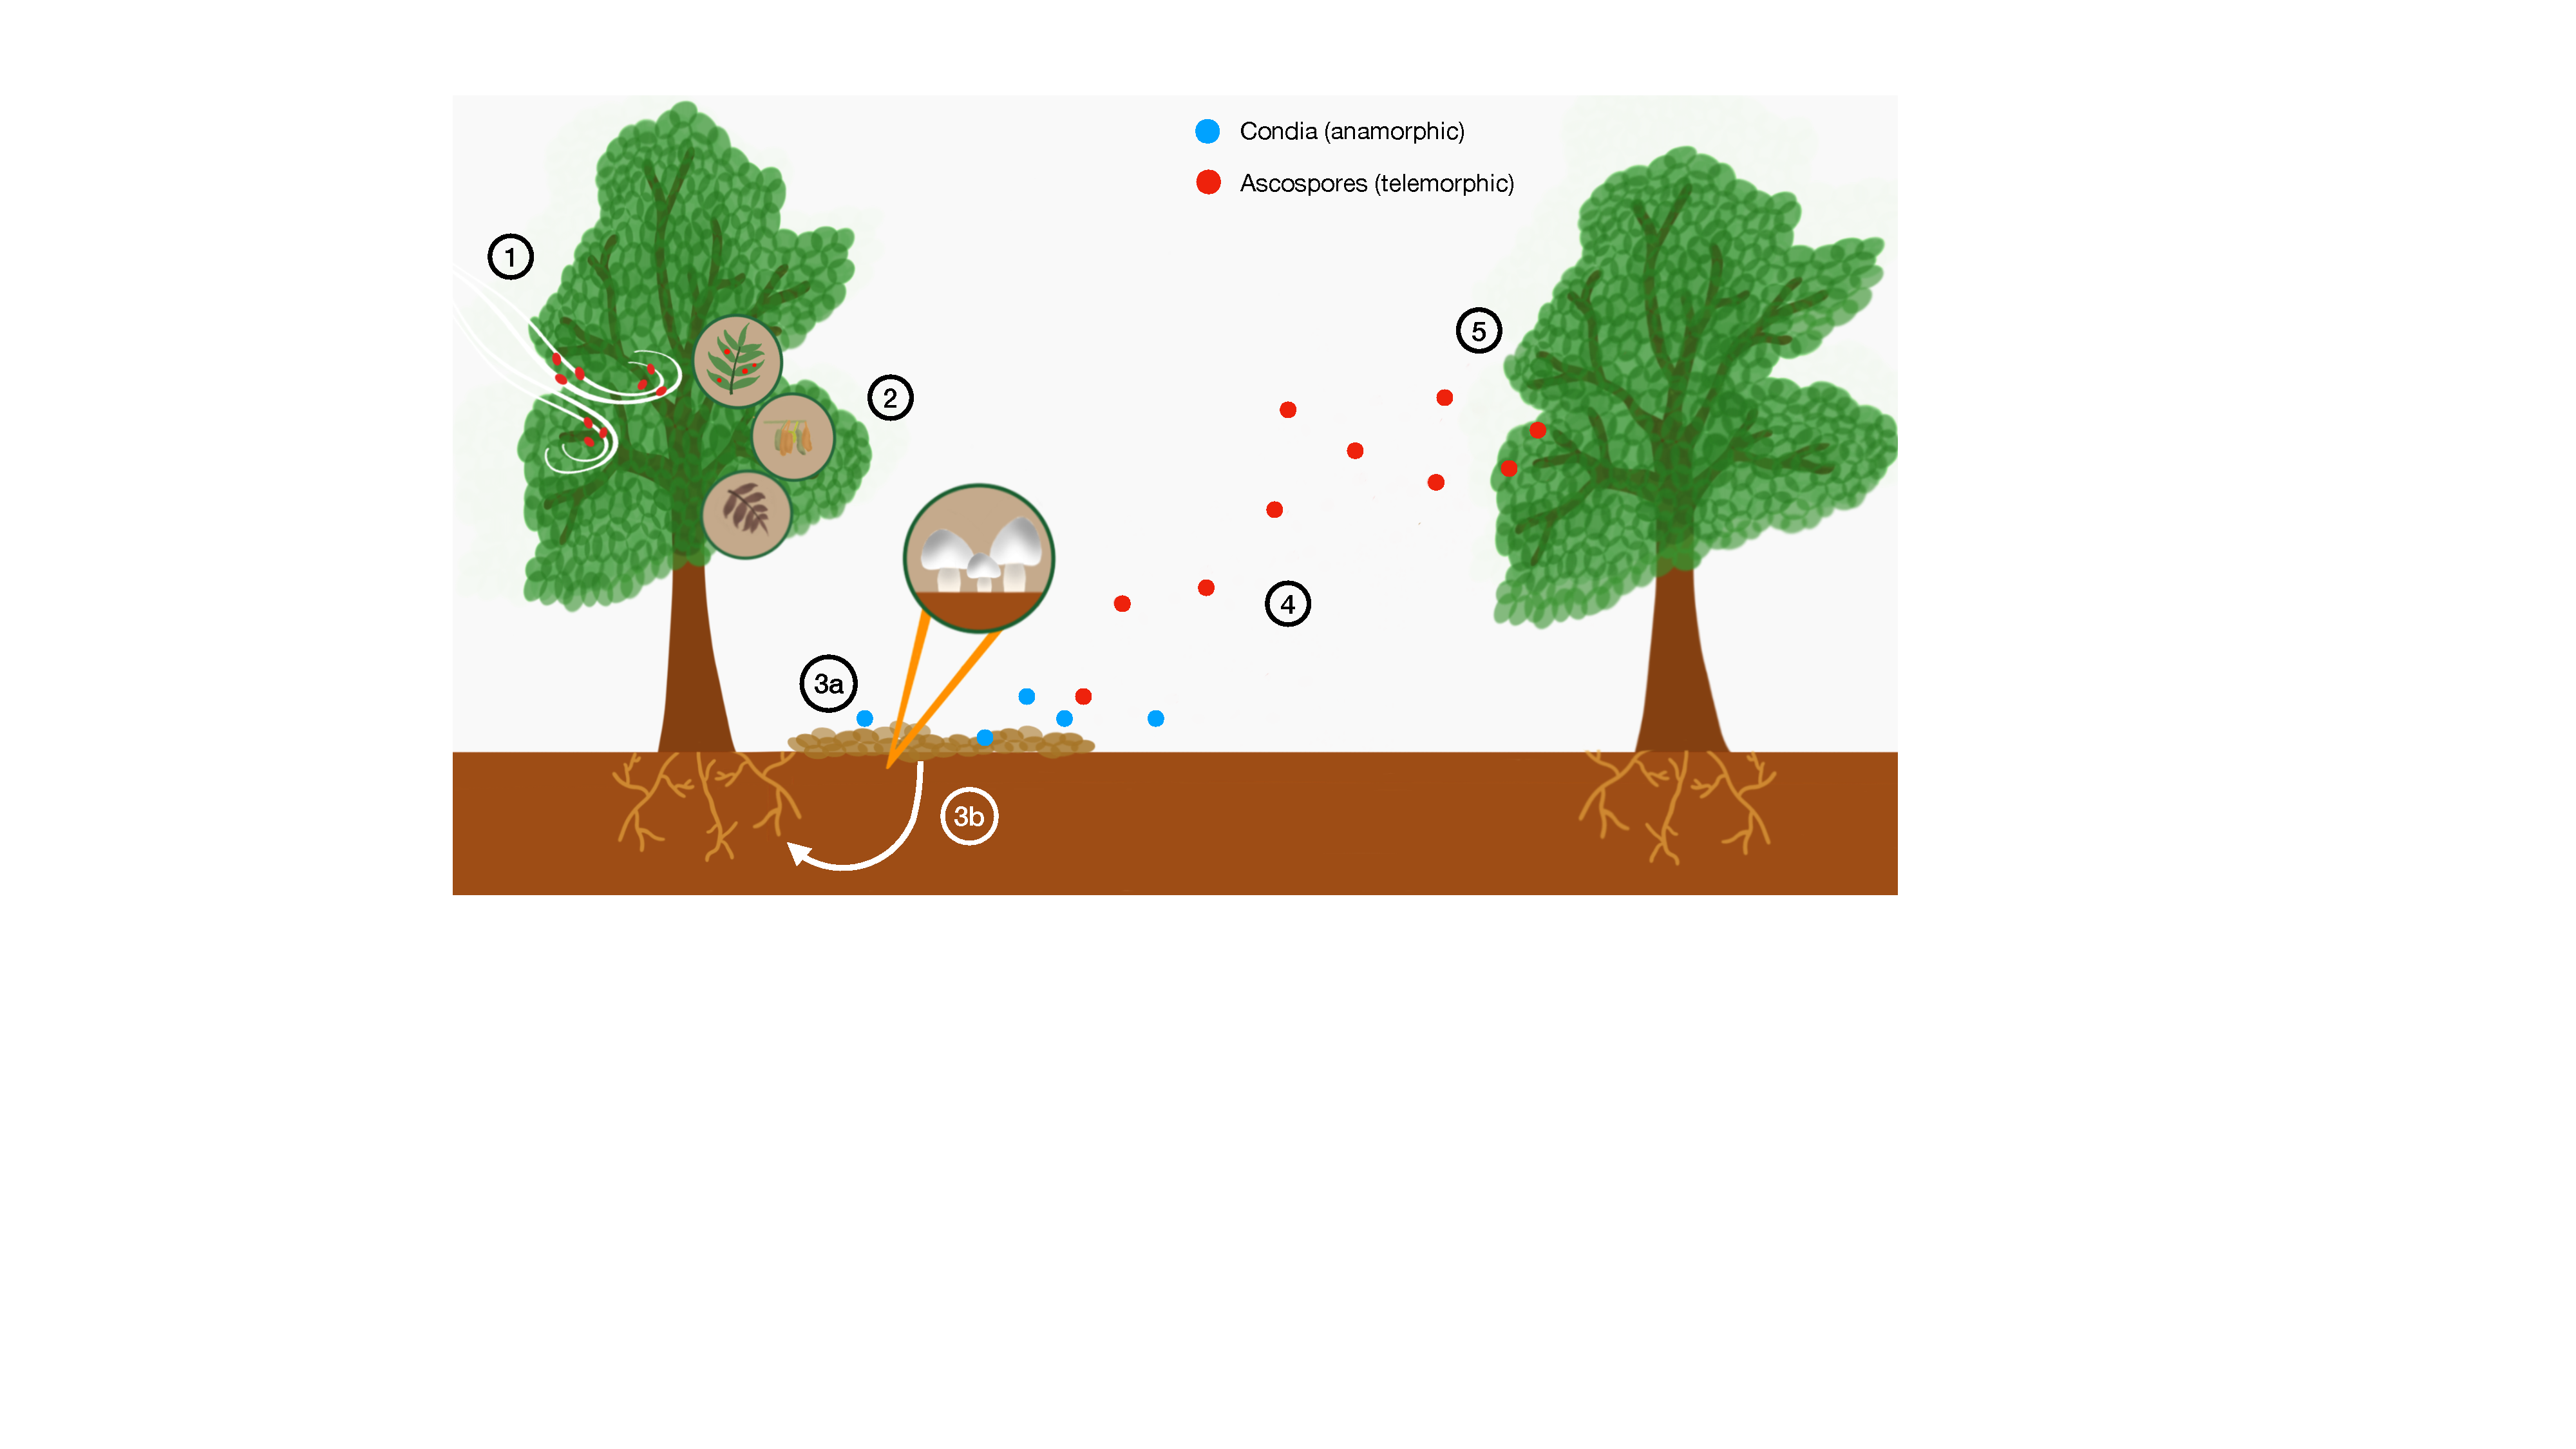
\includegraphics[scale=0.425]{chapter2/figures/ash-dieback-illustration.pdf}
    \caption{\textcolor{red}{describe ADB lifecycle} \blindtext }
    \label{fig:my_label}
\end{figure}

\newpage

\subsection{Dispersal}

In general, fungal spores have an efficient multi-scale wind-dispersal mechanism,
known to travel large distances \cite{golan2017long, wingen2013long, mundt2009aerial}
often described by power-law kernels, e.g. \cite{shaw2006assembling}.
From an epidemiological perspective, data on spore dispersal does not necessarily reflect the dynamics of new infections, 
as we cannot guarantee the availability of susceptible host material.
Even supposing available hosts, we cannot guarantee invasive spore colonisation.
However, studies on spore dispersal shed essential light on the spatial scale of ADB dispersal. 

Modern methods typically rely on `spore trapping' and real-time polymerase chain reaction (PRC) to study spores dispersal.
Data collected by \cite{chandelier2014detection} over three years using a (rotating arm) trapping system
and PRC amplification. The authors reported a $10\%$ spore trapping efficiency, and that most
dispersed ascospores remained within $50\mathrm{m}$ from the infectious source, with only a small number of spores exceeding 
distances beyond $50\mathrm{m}$. The work of \cite{chandelier2014detection} demonstrated the utility of novel PCR methods
to spore trap, but undesirably collected dispersal data over relatively small spatial scales.

Among the first landscape-scale fungal spore studies were conducted by \cite{long-range-dispersal}.
The authors focused on a comparable ascomycete fungus, \textit{Mycosphaerella fijiensis}, affecting banana plants.
Interestingly, \cite{long-range-dispersal} reported that asexual spore dispersal gradients extended 
a small distance $15\mathrm{m}$. As opposed to occasional, rare LDD in sexual (ascospore) dispersal up to $1000\mathrm{m}$.
Contrasting sexual and asexual spore dispersal was novel, and observing a small localised asexual dispersal gradient supports
the accepted idea that sexual dispersal in ADB is the dominant driver of disease spread.

Arguably the most comprehensive multi-scale study of ADB spore dispersal was performed by \cite{grosdidier2018tracking}.
In their paper, \cite{grosdidier2018tracking} tracked the local and landscape-level dispersal of ascospores
produced by \textit{H. fraxineus} in France.
The data collected relied on spore trapping and PRC; the reported trapping efficiency was $30–47\%$, marking an improvement over previous studies
e.g \cite{chandelier2014detection}. Most spores dispersal remained localised up to $50\mathrm{m}$ away from the inoculum source,
consistent with the results mentioned above put forward by \cite{chandelier2014detection}.
Nevertheless \cite{grosdidier2018tracking} set spore traps over much larger spatial scales ($\sim 100\mathrm{km}$),
subsequently detecting ADB spores $50-100\mathrm{km}$ ahead of the disease front.

Two dispersal kernels were used by \cite{grosdidier2018tracking}, a thin tailed Gaussian and an inverse 
power law of the forms:
\begin{equation}
    D(a, r) = \frac{1}{\pi a^2}\exp\big[-\frac{r^2}{a^2}\big]
    \label{eq:adb-ga}
\end{equation}
and
\begin{equation}
    D(a, r) = \frac{(b-1)(b-2)}{2\pi a^2}\big[ 1+ \frac{r}{a}\big]^{-b}
    \label{eq:geometric-invserse-power-law}
\end{equation}
where $a$ and $b$ are fitted parameters (for the Gaussian kernel, $a=\sqrt{2}\sigma$ with $\sigma$ being the standard deviation.). 
Equation \ref{eq:geometric-invserse-power-law} falls into the classical two-parameter geometric family of dispersal distributions.
The scale parameter is described by $a$ and the shape parameter by $b$. The mean dispersal distance described by Equation
\ref{eq:geometric-invserse-power-law} is  $\frac{2a}{b-3}$, and parameters $a$ and $b$ are valid for $a>0$ and $b>2$.

The functional form of Equation \ref{eq:geometric-invserse-power-law} is predicated on pollen dispersal studies,
as reviewed by \cite{nathan2012dispersal}. The tail of Equation \ref{eq:geometric-invserse-power-law} is 
particularly well suited to describe LDD events, as noted by \cite{https://doi.org/10.1111/j.1365-294X.2004.02100.x}
when describing the dispersal of pollen particulates. Moreover, a study by \cite{https://doi.org/10.1111/j.1365-294X.2006.03155.x}
used Equation \ref{eq:geometric-invserse-power-law} to model pollen-dispersal (and thus plant gene-flow) over landscape-level spatial scales. 
Presumably, the ability of Equation \ref{eq:geometric-invserse-power-law} to describe LDD, and the size similarity between pollen and fungi spores, 
motivated \cite{grosdidier2018tracking} to include it their field study. 
% A recent article published by \cite{golan2017long} presents an interesting system to 

\newpage

\subsection{Management and control}

Losing abundant ash populations could have dire consequences for several ecosystem functions, 
including nutrient recycling, food webs, and biodiversity.
As such, ADB presents a conservation challenge throughout Europe and Great Britain \cite{pautasso2013european}.
Moreover, under the rapid proliferation of ADB, various ash-dependent species risk extinction;
\cite{hultberg2020ash} identified $115$ at-risk (lichens, fungi, invertebrates, bryophytes/moss) species in Sweden that rely on ash.
Alarmingly, many of the ash-associated species identified by \cite{hultberg2020ash} also depend on elm species, which in turn face 
the fungal pathogen Dutch elm disease \cite{brasier1991ophiostoma}.

Given the ecological importance of ash in numerous temperate European forest types (e.g. floodplain, ravine, 
and lowland \cite{dobrowolska2011review}), management and pathogen control remain essential. The control of ash dieback
in a well-established focus of infestation, in both natural and artificial environments, is virtually impossible
\cite{havrdova2017environmental}, and it is already well recognised that ADB will eventually wipe out the vast 
majority of ash in Great Britain \cite{ash-dieback-costs}.

Controlling the spread of ash dieback reflects the spatial and temporal scale over which it spreads.
In particular, ADB fungal spores are thought to be able to jump between patches of ash,
even in the absence of susceptible hosts \cite{wingen2013long}.
However, LDD accounts for only a small minority of spore dispersal.
Furthermore, despite many notions of LDD, no unified LDD classification system exist, 
which led \cite{golan2017long} to propose a definition based on the distance traversed by the top $1\%$ of spores.

The long-term survival of ash depends on a small proportion of genetically resistant ash trees.
Despite many unpublished reports, genetic tolerance studies only began surfacing around a decade
after the widespread outbreak \cite{kjaer2012adaptive, stener2013clonal, mckinney2014ash}.
In particular, \cite{doi:10.1094/PHYTO-11-15-0284-R} showed the heritability of crown dieback and
collar-lesion symptom expression. In the three French provenances sampled,
\cite{doi:10.1094/PHYTO-11-15-0284-R} found no evidence for regional tolerance.
Presently, genetic tolerance is widely accepted \cite{havrdova2016differences, skovsgaard2017silvicultural},
and more recent work has focused on metabolomic tolerance classification,
profiling which metabolite markers correlate with resistance 
\cite{nemesio2020canditate, nemesio2020metabolomics, sidda2020diversity, chaudhary2020identification}.

A silvicultural system proposed by \cite{skovsgaard2017silvicultural} involves visually scoring severity based on crown dieback
and collar lesions. In this scheme, forest managers would inspect disease severity to record disease progression over time
and record genetically resistant trees to cultivate for future timber production. In addition, 
\cite{skovsgaard2017silvicultural} proposed that diseased forest stands should not be indiscriminately felled on account of high-value
tolerant individuals; this suggestion stands in contrast to the idea of a `cull radius', as alluded to by \cite{WEBIDEMICS}. 
In general, felling infected stands is ill-advised  \cite{chandelier2017ash}, except when infected hosts present a risk of uncontrolled 
and damaging tree-fall\textemdash as explained by \cite{ash-dieback-costs} when assessing the clean-up cost within Great Britain.

Following the establishment of genetic tolerance, numerous long-term preservation strategies 
rest on cultivating and replanting trees that exhibit low damage levels. Breeding 
programs in many European countries are currently underway, as reviewed by \cite{https://doi.org/10.1002/ppp3.10060}.
In the UK, the Living Tree Project (https://livingashproject.org.uk) aims to collate tolerant UK ash for future breeding.

% \cite{ash-tree2}
% - Approaches to conservation differ between forest and commercial ash stand \cite{skovsgaard2017silvicultural}. 
% - Among the control strategies, application of fungicide to infected biomass has been shown effective \cite{hauptman2015application}
% Among LDD human-mediated.
% - read me ->

% - statistical modelling work has shown the importance of environmental factors in the spread of disease \cite{dal2014risk, chumanova2019predicting}
% - the risk of spread.. was conduced by \cite{fellenor2019ash}....
% - \cite{dal2015epidemiology} un-published thesis

% 3) The construction of the simple lattice model
% -----------------------------------------------------------------------------
% 1) Introduce toy percolation model
% 2) Include stochastic infectivity parameter
% 3) Show behaviour in one and two dimensions
% 4) Set the basis model and establish the main ensemble method 
% -----------------------------------------------------------------------------

\chapter{Tree disease: a simple lattice model}
\label{chapter:SLM}

Typically, models of tree disease are complicated and involve multiple parameters informed by experimental data. Moreover, modelling a specific pathosystem requires in-depth, specialist knowledge to incorporate biological realism, such as pathogen lifecycles or environmental suitability. This introductory chapter outlines a simple model of tree disease spreading through a forest that will lay the foundations for more detailed treatment in later chapters.
Consequently, the compartmentalised $SIR$, percolation-based, model used by \cite{OROZCOFUENTES201912} will be recounted. 

From the first principles, the percolation model will be analysed over one parameter, tree density $\rho$.
Thus, leading to a mathematical and conceptual definition of percolation in the context of tree-based epidemics. 
The simple one-parameter model will then give way to a discussion of criticality and self-similarity in the system;
the discussion will include a summary of critical phenomena and some universal behaviour within the model.
Crucially, this chapter demonstrates the importance of thresholds in the spread of tree-based diseases.

Having established a simple one-parameter model, a more involved two-parameter `stochastic percolation' model will be developed and examined. 
Stochastic percolation will include an extra parameter representing the degree of pathogen infectivity. 
In general, measuring infectivity is challenging and subject to much spatial and temporal variation, such as changing climatic/environment conditions or species-level genetic variations in susceptibilities.  
However, including a stochastic infectivity parameter is essential to construct representative models of tree-based epidemics, as infectivity (or susceptibility) can vary widely over a landscape.
The two-parameter model will constitute a simple lattice model (SLM) of disease dynamics. 
This introductory chapter will introduce an ensemble-averaging method used throughout the thesis;
in the present case, ensemble-averaged parameter sweeps are used to categorize the SLM behaviour.

\section{Percolation formalism}
% understand universality class and scaling exponents 
% we consider small timescales and neglect regrowth factors
Consider a square lattice of size $L \times L$ , where each site in the lattice can be in one of two states: %
open with probability $\rho$ or closed with probability ($1-\rho$). %
Therefore, the probability $\rho$ describes a density parameter and encapsulates the occupancy of a homogeneous distribution of open and closed lattice positions.
One open site ($c_p$) is connected to another ($c_q$) if laid within the Von Neumann neighbourhood \cite{toffoli1987cellular}.

A connected set of open nearest neighbours define a cluster denoted by $C$, where $c_i \in C$.
Given the set $C$, it is possible to traverse between member sites $c_i \in C$ by moving through the lattice in either horizontal or vertical steps `Von Neumann motion'. 
Given two distinct non-overlapping clusters $c_i \in C_1$ and $c_j \in C_2$, then $c_i \neq c_j $ i.e. there is no way to jump from $C_1$ to $C_2$ following Von Neumann motion. 
Connectivity is defined between lattice sites rather than the edges which connect them, known as `site' percolation\textemdash as opposed to `bond' percolation.

If $\rho$ is close to zero, only small clusters would be present as a disordered system; 
conversely, if $\rho$ is large, a connected network of open positions would dominate the domain, thus defining an ordered system.
At some point for $\rho \in [0, 1]$, a critical threshold ($\rho_c$) would be reached, and a singularity of connected sites would span an infinite sized lattice.
On a finite lattice, the cluster is said to percolate and form a `spanning cluster' ($C_\infty$) that extends between at least two different edges of the lattice.
The formation of the spanning cluster occurs abruptly between a very narrow range of $\rho$ values. 
Therefore, the threshold for percolation defines a critical-point \cite{STAUFFER19791}. 

The critical point can be defined as the least value of $\rho$ where percolation occurs with non-zero probability. %
This can be formalised by first considering the probability function: $\theta (\rho)= \lbrace \rho:|C|=\infty\rbrace$ where $\theta(\rho)$ is the probability of an arbitrary site, %
within a lattice of density $\rho$, belonging to cluster $C$ of size $\infty$ (i.e. the spanning cluster). %
The critical value then satisfies: %

\begin{equation}
\label{eq:critical_threshold_1d}
    \rho _{c}=sup \lbrace \rho : \theta (\rho ) = 0 \rbrace
\end{equation}

At this point, the spanning cluster has been described conceptually, although many nuances and technicalities complicate the definition. %
For example, the probability of percolation has a non-trivial dependence on the size of the lattice;
if the mean cluster size, defined by a `characteristic' cluster length $C_r$, is above or comparable to $L$, 
percolation could occur despite the density residing in the sub-critical regime. %
The size of the lattice is therefore required to be sufficiently large compared to individual lattice positions (or microscopic interactions) 
in order to approximate the threshold ($\rho_c$) reliably and produce a spanning cluster ($C_{\infty}$). 

When the domain size is large, the threshold $\rho_c$ will remains approximately constant and insensitive to small changes in the domain. 
All proceeding simulations in this chapter are conducted on finite-sized domains between two and three orders of magnitude larger than individual lattice points.
The model presented in this chapter (first published by \cite{OROZCOFUENTES201912}) was 
found to agree with the accepted percolation threshold, when the lattice had size $L \sim 500\times500$;
the lattice configuration used here will therefore assume the same size configuration. 

Intuitively, it is clear to see the link between percolation and epidemiology: 
open lattice positions act as susceptible members of a population ($S$), and $\rho$ defines a density of the hosts. 
In this paradigm, the spanning cluster describes a high-impact epidemic that spreads uncontrollably. 
Small to medium-sized clusters existing at (or slightly below) the threshold describe short-lived, 
failed epidemics where the pathogen spreads for a time before becoming extinct.

These analogies have clear limitations when describing mobile hosts, but fortunately, trees are sessile and immobile.
Thus, percolation theory provides a valuable framework for modelling tree diseases (see Chapter \ref{section:lit-rev-perc} 
for a review of percolation-based models). 
Forming a percolation-based lattice model of tree disease requires us first to combine a compartmental $SIR$-like model within the lattice ($L$) mentioned above. %
Next, an appropriate transmission dynamic is described to model the spread of disease between lattice points.


\section{Percolation-based $SIR$}

The percolation density parameter ($\rho$) defines a simple host distribution.
Namely, $\rho$ represents the probability of a susceptible tree $S$ (given a numerical value $1$), 
while empty lattice positions define an insusceptible state $\emptyset$ (with numerical value $0$).
If a susceptible tree neighbours an infected tree, it will transition into the $I$ compartment (having a numerical value of $2$).
Transitions between states occur with a probability of 1, and the Von-Neumann neighbourhood describes the connectivity between trees.
After an arbitrary number of time-steps $T$, an infected tree will transition into the removed state $R$ and die; 
see appendix \ref{a:propagation} for more information on the numerical implementation. %
For simplicity, the infectious lifetime will not be considered as a parameter but will remain fixed at $T=1.0$\textemdash revisited below in section \ref{ch3:two-param-model}.

The initial conditions begin with a small patch of infected hosts (of size $5\times5$) located at the origin ($L_O$) at $t=0$, and percolation events describe the boundary conditions. 
Percolation occurs when the infection spreads from $L_O$ to any of the four lattice boundaries;  thus defining a connected cluster of infectious-removed that spans the domain from $L_O$.
Each time-step through the simulation represents an arbitrary unit of time, and simulation termination occurs on one of three boundary conditions: 
1) a percolation is observed 
2) the pathogen becomes extinction 
3) a time-horizon of $N$ steps is reached. 
Typical simulations on a domain of size $500 \times 500$ are shown in Figure \ref{fig:ch3-perc-spread} through three time-steps. 

\begin{figure}
    \centering
    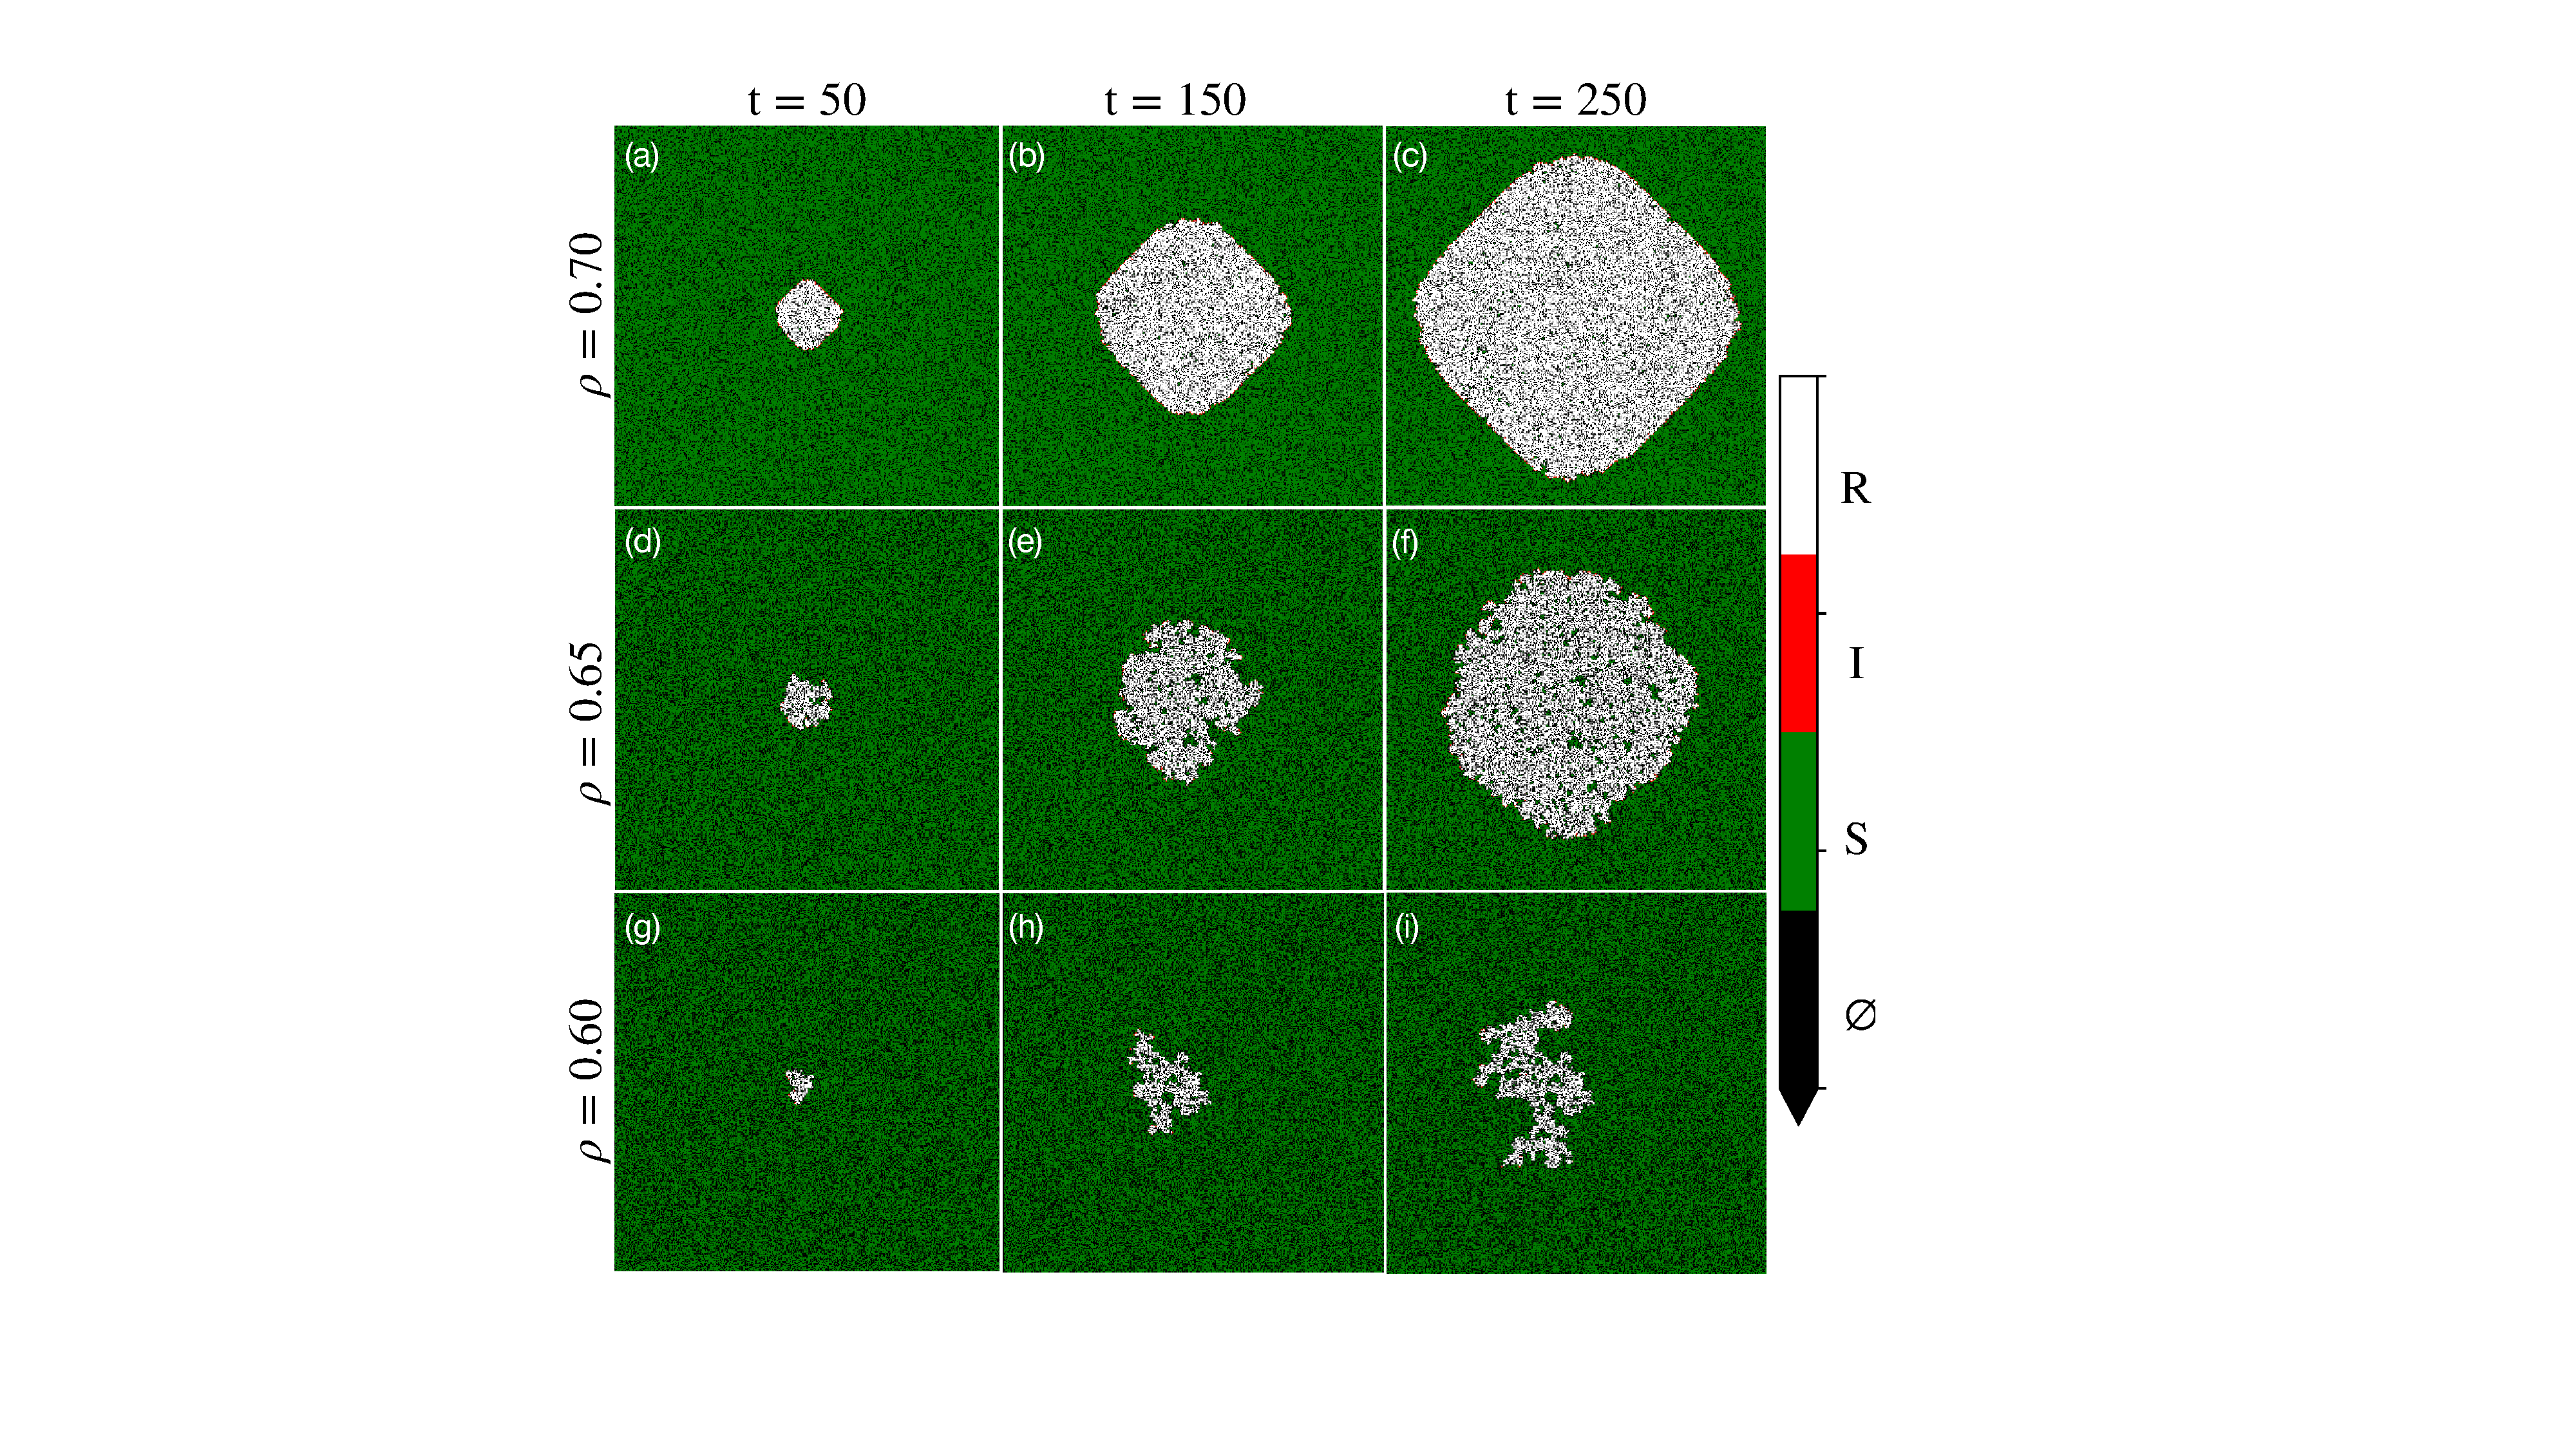
\includegraphics[scale=0.50]{chapter3/figures/figure1-1param-perc.pdf}
    \caption{
        Evolving outbreaks in the one-parameter, percolation-based $SIR$ model are shown for different tree densities ($\rho$).
        From left to right, three successive time-steps are plotted on a domains of size $500 \times 500$.
        Green and black pixels represent susceptible and insusceptible (empty) host units, respectively, 
        while white and red lattice sites depict removed and infectious hosts. 
        (a-c) High-density simulations reveal an unnatural diamond-shaped spread, undesirably reflecting the underlying lattice geometry.
        (d-f) Simulations above the threshold spread radially outward from the epicentre, defining a connected cluster of infectious-removed trees in the process. (g-i) Around the percolation threshold, the disease spreads slowly and chaotically outward. 
        }
    \label{fig:ch3-perc-spread}
\end{figure}

Figure \ref{fig:ch3-perc-spread} illustrates dynamic simulations of disease spread through a 
series of $500 \times 500 $ domain. At density $\rho=0.70$, Figures \ref{fig:ch3-perc-spread} (a-c)
reveal an unnatural diamond-like pattern of spread reflecting artefacts of the lattice geometry.
In theory, the diamond-like spread would look different if the lattice geometry is changed\textemdash a
triangular or honeycomb lattice, for example. The diamond-like spread begins to disappear in 
Figure \ref{fig:ch3-perc-spread}(d-f), when simulations have density $\rho=0.65$.
At this density, a wave-like propagation of infected trees spread radially from the epicentre outward 
toward the lattice boundary and look more realistic.
Interestingly, these observations can be understood through the lens of stochasticity. At a lower tree density, the probability of 
spread between neighbours is lower, and the spread is more chaotic, thus disrupting the highly ordered wavefront shown 
through panels (a-c) into a circular travelling wavefront.

Figure \ref{fig:ch3-perc-spread}(g-i), show the spread of disease for a lower host density of $\rho = 0.60$.
As the disease spreads outward, a more fractal-like pattern begins to emerge.
Moreover, the disease spreads slowly, as evidenced by the smaller area traced by the infectious-removed trees shown from white to red.
In this regime of spread, `persisting' simulations result from the slowly evolving epidemic as it defines a disordered cluster of infectious-removed hosts.
\newpage

\subsection{Percolation threshold}
\label{section:universality}

Suppose simulations begin at low density, below the threshold; in this case, evolving epidemics are unlikely to percolate to the domain boundary, and the pathogen will become extinct.
If the host density increases, we can imagine that epidemics begin percolating to the boundary for some specific value.
Consequently, the probability of percolation was examined over a sweep of density parameters, shown in Figure \ref{fig:ch3-perc}(a).
Unsurprisingly, a threshold-like behaviour is revealed.
All the simulations that form Figure \ref{fig:ch3-perc}(a) evolved inside a $500\times 500$ sized domain.
The probability of percolation ($Pr(\rho)$) defines
a critical region, highlighted in orange (where $ \rho \in [0.57, 0.62$]), that separates regimes of pathogen extinction and percolation/epidemic.
The threshold depicted by Figure \ref{fig:ch3-perc}(a) is consistent with the accepted percolation threshold for a two-dimensional square $\rho_c \approx 0.592$.

The value of $Pr(\rho)$ depends non-trivially on stochasticity, which motivated an ensemble-averaged approach\textemdash 
further reading on the underlying theory of ensemble-averaging can be found in \cite{gibbs1902elementary}.
In Figure \ref{fig:ch3-perc}(a), 100 repeated simulations obtain the probability of percolation. Simulations that percolate to the domain boundary assume the numerical value of one, while pathogen extinction events assume zero; for each value of $\rho$, the average value is computed, thus defining a probability $Pr(\rho)$.

At the critical density, denoted by $\rho_c$, we witness the emergence of some exciting phenomena.
Figures \ref{fig:ch3-perc}(c-d) show a spanning cluster ($C_\infty$) of infectious and removed trees (in white to red respectively) at $\rho_c=0.592$.
The cluster looks remarkably similar at all spatial resolutions, said to be `self-similar' \cite{Kapitulnik_1983}.
Within $C_\infty$, one can identify clusters of untouched susceptible trees (in green) of various sizes, suggesting a distribution of cluster sizes occupy all possible length scales.
In the literature, clusters can be described by a `cluster number' ($n_s$) distribution, where $n_s$ is the number of clusters containing $s$ open/susceptible lattice sites.
Furthermore, around the percolation threshold, there can be significant fluctuations in the size of the clusters formed\footnote{
The related statistical fluctuations analysed by \cite{OROZCOFUENTES201912}
present an effective early warning system for the prediction of forest-based pathosystems\textemdash revisited in the next chapter.
}.

\begin{figure}
    \centering
    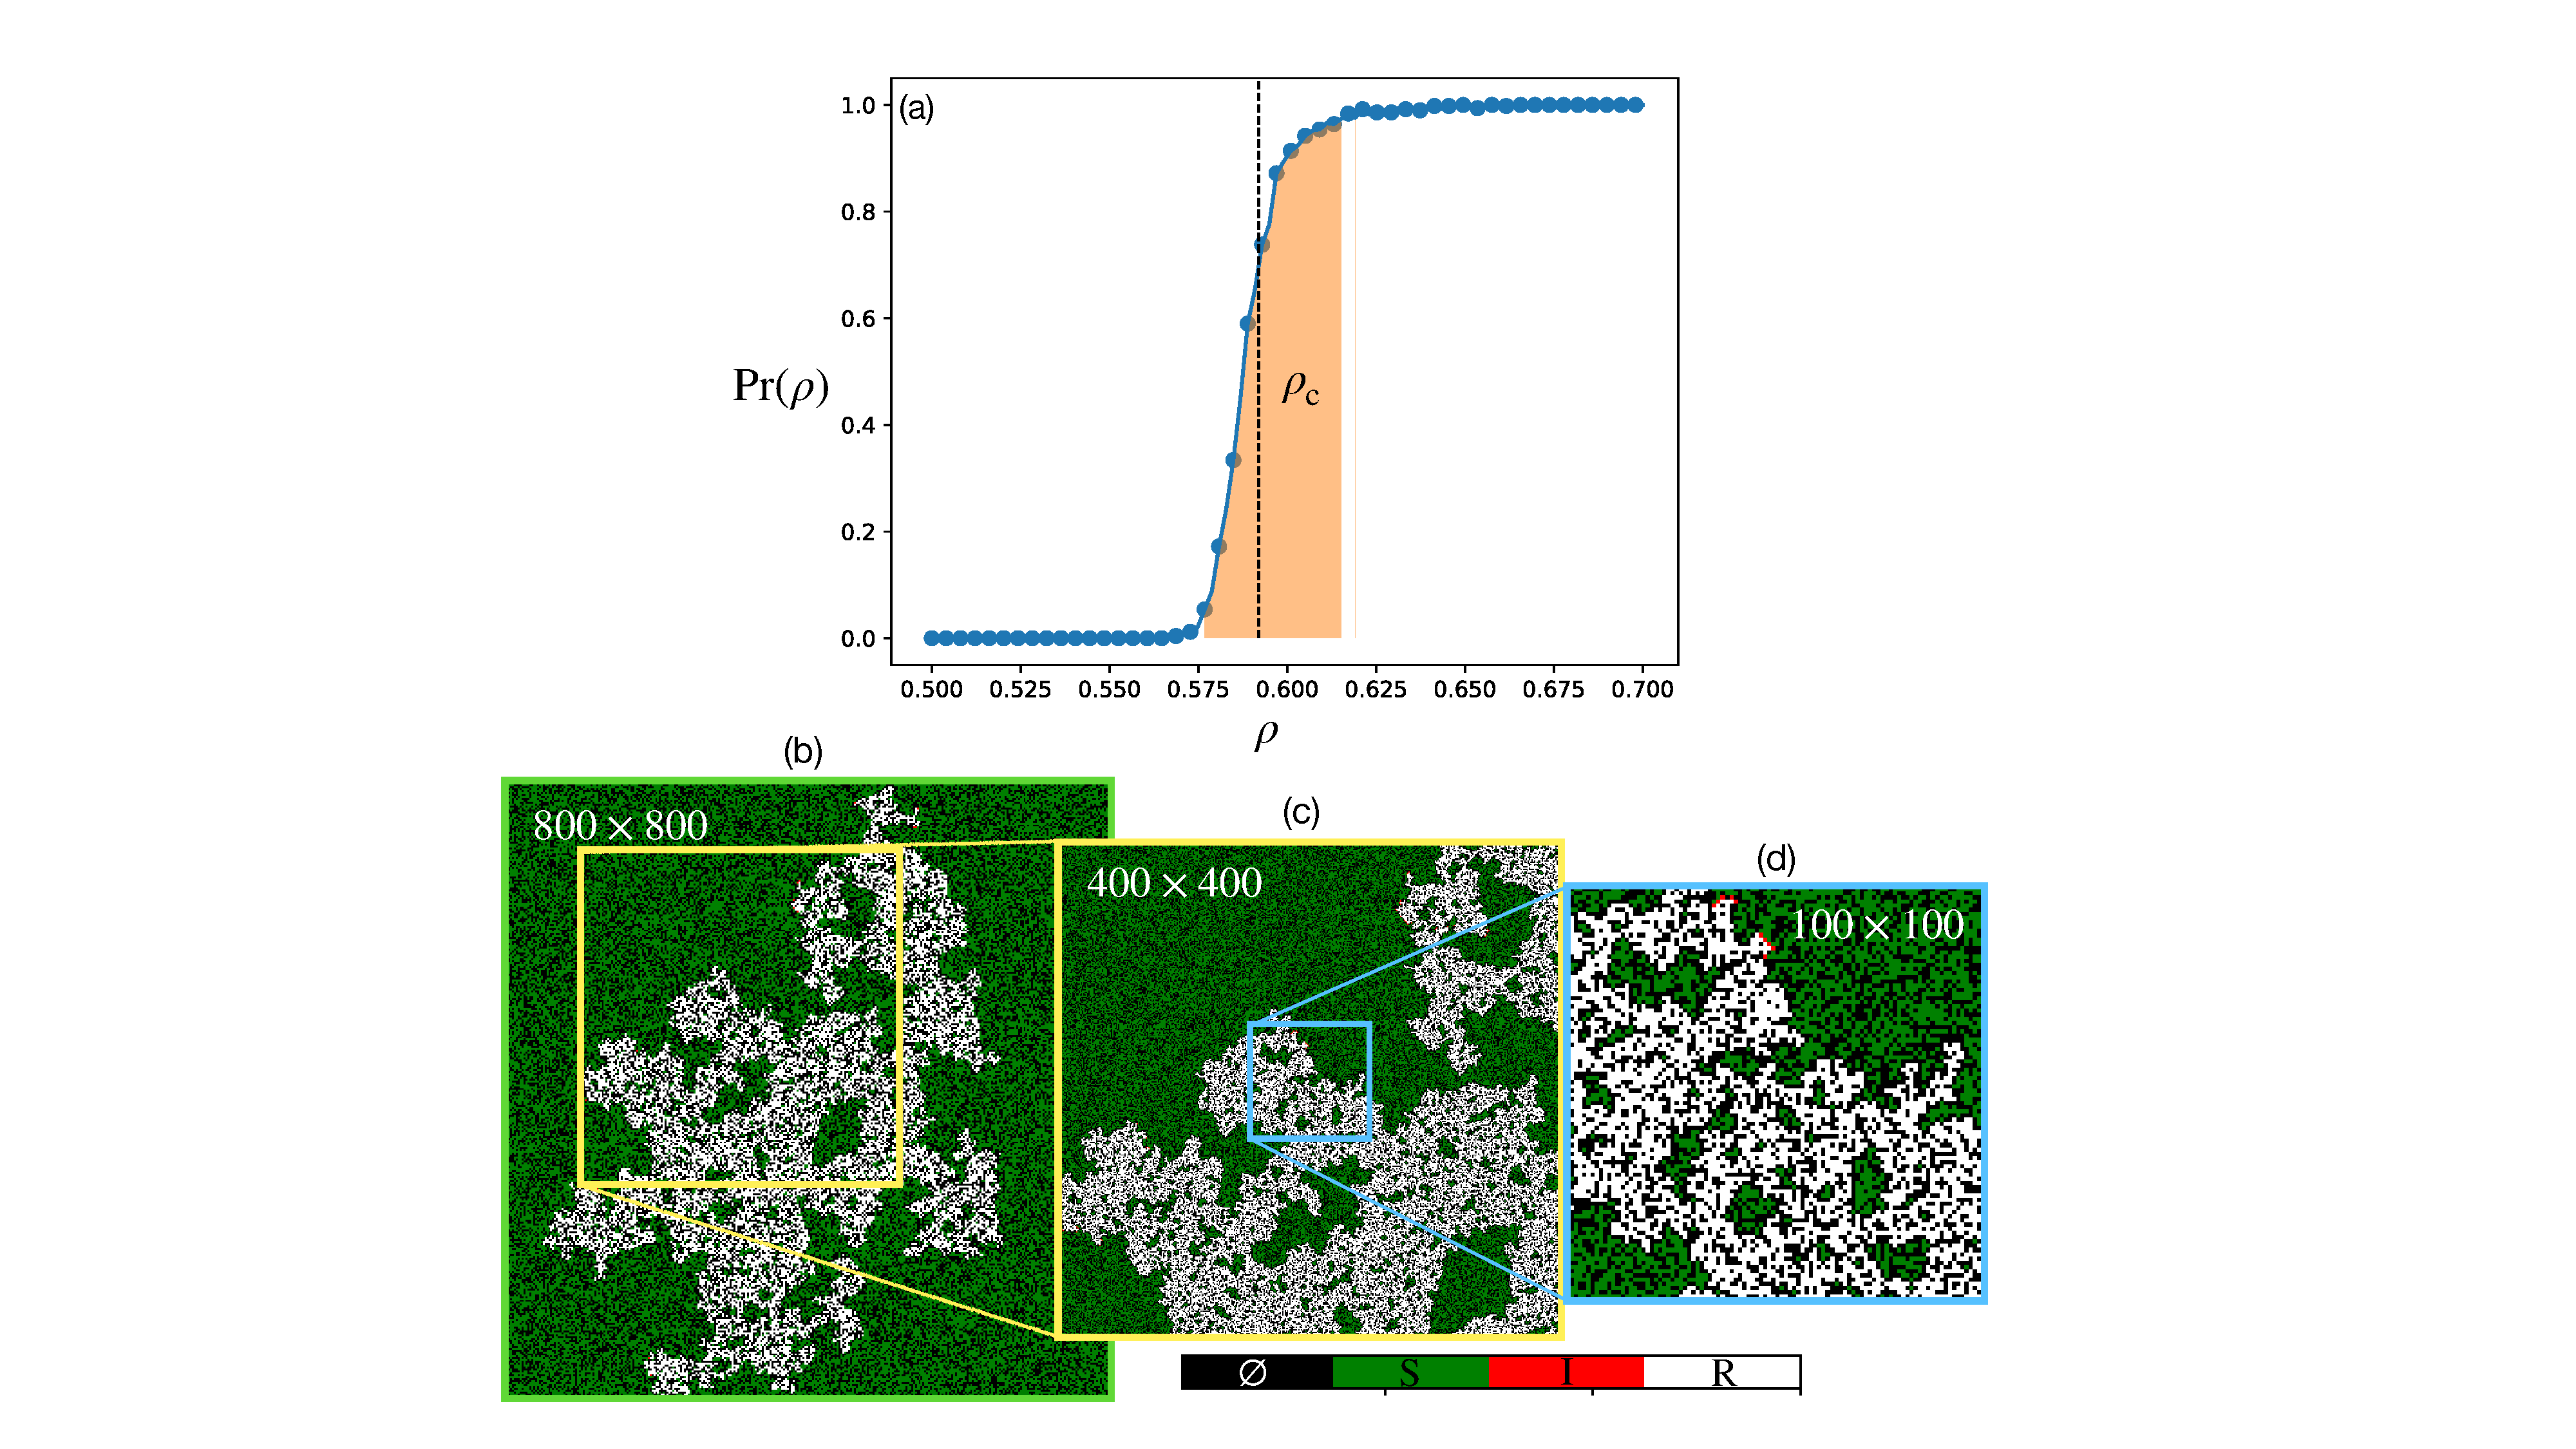
\includegraphics[scale=0.4]{chapter3/figures/figure2-1param-perc-threshold.pdf}
    \caption{The percolation threshold is determined for the one-parameter percolation $SIR$ model.
            (a) The probability of percolation ($\mathrm{Pr(\rho)}$) is plotted against host density.
            The shaped orange region highlights a threshold consistent with results from classical percolation theory, 
            namely $\rho_c = 0.592$, shown by the vertical dashed line. 
            (b-c) At the critical density $\rho_c$, a cluster spanning the domain in (b) is assessed over progressively smaller resolutions.
            Similar features are observed on different scales and scale invariance is observed in the model.
            }
    \label{fig:ch3-perc} % \label{fig:ch3-perc-pr}
\end{figure}

\begin{table}[h!]
  \begin{center}
    \begin{tabular}{l|c|c|r} % <-- Alignments: 1st column left, 2nd middle and 3rd right, with vertical lines in between
    \hline
      \textbf{Lattice} & NN & \textbf{Site percolation} & \textbf{Bond percolation}\\
      \hline
      1D & 2 & 1 & 1\\
      Square 2D & 4 & 0.593 & $1/2$\\
      Triangular 2D & 6 & $1/2$ & 0.347\\
      Honeycomb & 3 & 0.696 & 0.653\\
      Diamond & 4 & 0.43 & 0.388\\
      Voronoi & - & 0.714 & 0.667\\
    \hline
    \end{tabular}
    \caption{The site and bond percolation threshold for various lattice types\textemdash data published by \cite{stauffer2018introduction, PhysRevE.80.041101}.
            Each lattice configuration defines a set of nearest neighbours (NN).
    }
    \label{tab:perc}
  \end{center}
\end{table}

This chapter rests on a square lattice, although we could have considered many other configurations, e.g. a triangular, honeycomb or Voronoi lattice.
From the observation of Figures \ref{fig:ch3-perc-spread}(a-c),
high host densities would produce highly ordered wavefronts reflecting the different lattice configurations.
In addition, various quantities within the model would change, especially the critical density $\rho_c$ that changes in response to the nearest neighbour (NN) number.
For completeness, table \ref{tab:perc} shows a selection of site and bond percolation thresholds.
Even though $\rho_c$ would change between lattice configurations, some universal properties of the model would remain fixed, 
which leads to a description of universality below.


\subsection{Universality}

At $\rho \sim \rho_c$, percolation and scaling theory explain how the system follows a power law of the form $\propto (\rho - \rho_c)^{\alpha}$ 
where $\alpha$ is a universal critical exponent.
All systems that possess the same exponent are members of the same `universality class' \cite{PhysRev.180.594, RevModPhys.76.663}.
Consider the probability that one open site (at the origin) is connected to another open site a distance $r$ away. %
In this scenario, the probability is described by the `correlation function' $g(r)$. %
The behaviour of this function defines a length scale, denoted as the `correlation length' $\xi$ that dictates how the probability of `connectedness' decays with distance $r$. %
For densities close to percolation threshold: %
\begin{equation}
    \xi \sim |\rho - \rho_c|^{-\nu}
    \label{eq:universal-scaling}
\end{equation}
where $\nu$ is a critical exponent that is universal for all lattice configurations and only depends on the dimension of the lattice used. In general, there are critical exponents for other quantities, e.g. cluster sizes\textemdash discussed more below. 
However, all follow similar power laws, as shown by \cite{stauffer2018introduction, STAUFFER19791}.

Equation \ref{eq:universal-scaling} can be understood by exploring how the connectivity of open sites depend on the density and the divergence that occurs at the threshold $\rho=\rho_c$. 
For low densities, $\xi$ is small because all clusters exist in singlets/triplets.
However, as $\rho$ increases, the mean cluster length increases as more sites become open and connect to form larger clusters. 
As we approach the critical density (from the direction $\rho \rightarrow \rho_c^{-}$) the spanning cluster is formed and $\xi$ diverges towards infinity, $\xi \rightarrow \infty$. 
If one neglects the divergent spanning cluster, a similar picture is painted for densities just above criticality $\rho > \rho_c$. 
That is, the correlation length $\xi$ decays rapidly as $|\rho - \rho_c|$ increases. 
This time however,  mid-to-large sized clusters get absorbed by $C_\infty$ as the density increases;
thus leaving only small untouched clusters, as $\rho \rightarrow 1$ and $\xi \rightarrow 0 $. 
See \cite{STAUFFER19791} for a detailed breakdown of power laws and correlation length.

Lastly, it is worth discussing well-known results on how the cluster sizes (or masses) scale with the lattice dimension. 
If $\rho > \rho_c$, the largest cluster present (denoted by $M$) would scale according to $M\propto L^{2}$, cf. the evolving epidemics above the threshold in Figure \ref{fig:ch3-perc}; 
in contrast, if $\rho = \rho_c$, $M$ would follow $M\propto L^{1.9}$, 
where $d_F=1.9$ describes the cluster fractal dimension.
If we normalise the cluster by the size of the lattice ($L^2$), the mean density of $M$ will decay as the lattice size increases, i.e. $L^{1.9}/L^2 = L^{-0.10}$. 
Broadly, the critical phenomena found in percolation theory, thermodynamics and magnetism have close ties and are described by similar power laws underpinned by scaling theory \cite{Essam_1980}.

% If the system crosses the percolation threshold, it can be likened to a phase-transition. %
% Subsequently, the terms `phase-transition' and `percolation' will be used interchangeably throughout this work. 


\section{Pathogen infectivity}
\label{ch3:two-param-model}

We have established a percolation-based model of tree disease described by a one-dimensional parameter-space over tree density $\rho$. %
We now extend the parameter-space to include an `infectivity' parameter, denoted by $\beta$. %
Previously, we made an implicit assumption about pathogen-transmission, namely: 
infected trees will transmit the infection to susceptible nearest neighbours with perfect fidelity, that is, a probability of $1$. 
In reality, a pathogen may display a range of virulence depending on the environmental suitability or host susceptibility; 
exemplified by the pathogen ash dieback, known to cause more host damage in naturally occurring forest ecosystems \cite{marciulyniene2017can} 
and release more fungal spores conditional on temperature \cite{chandelier2014detection}.

To model infectivity, the parameter $\beta$ is introduced. The probability of a susceptible tree becoming infected during a single time-step is given by: $Pr(S \rightarrow I) = \beta$. Appendix \ref{a:propagation} contains more descriptive information on the computational implementation. 
The infectivity parameter describes a transmission `rate' (i.e. per time-step) and is closely linked to the infectious lifetime $T$ of the tree. %
If a susceptible host falls within a von Neuman neighbourhood of an infected host, it will remain susceptible with probability:
\begin{equation}
\label{eq:pr_s_s}
    Pr(S \rightarrow S) = \rho(1 -\beta)^T
\end{equation}
where $T$ is the number of an infectious lifetime;
thus, the probability of remaining susceptible decreases as the infectious lifetime gets larger.
Equation (\ref{eq:pr_s_s}) sets the scene for a predictive mean-field theory.
Subsequently, appendix \ref{a:slm-mean-field-theory} outlines steps toward a novel continuum model of tree disease.


Previously in the one-parameter $SIR$ variant, the infectious lifetime played a minor role in determining wavefront because pathogen transmission occurs with a probability of one.
However, now a susceptible host will survive for $t=T$ time-steps before transitioning into $R$. Ultimately, the model is non-dimensionalised, and the value of $T$ is arbitrary; however, a single step can be envisioned to be on the order of years.
At this stage, we have recovered the two-parameter model used by \cite{OROZCOFUENTES201912}, henceforth referred to as the `\textit{simple lattice model'} (SLM). 

Figure \ref{fig:slm} show three SLM simulations, spreading for the shown infectivity parameters through different time-steps.
All simulations in Figure \ref{fig:slm} are governed by a fixed value of $T=10$, and density $\rho=0.70$.
The colour bar in Figure \ref{fig:slm} represents different steps through the infectious period, from yellow to red.
Higher values of $\beta$ yield a faster spreading velocity,
as expected.
Figures \ref{fig:slm}(g-i) allude to $\beta$ altering the percolation threshold, on the basis of $\beta=0.25$ reflecting a more fractal-like spreading pattern, even well beyond the standard percolation threshold of $\rho_c=0.592$.

% Link  \cite{gilligan2008epidemiological} to the critical point

Figure \ref{fig:slm-wave-front} shows how variations in the infection lifetime can change the wave-front properties. 
The value of $\beta$ predominantly controls the speed of the wave-front, whereas $T$ controls the lag-time on the removal front. 
Therefore, increasing $T$ yields an increase in the wave-front thickness;
this is valid for $\rho > \rho_c$.
Around the percolation threshold $\rho \sim \rho_c$, the relationship between $T$ and spreading velocity is less obvious. 
Close to the percolation threshold, variations in $T$ have more importance, as it could lower or raise pathogen transmission below or above percolation thresholds, respectively.
If $T$ is held fixed, the critical threshold definition can now be generalised from Equation (\ref{eq:critical_threshold_1d}), to include the parameter $\beta$: 

\begin{equation}
\label{eq:critical_threshold_1d}
    \rho _{c}=sup \lbrace \rho, \beta : \theta (\rho, \beta ) = 0 \rbrace
\end{equation}

\begin{figure}
    \centering
    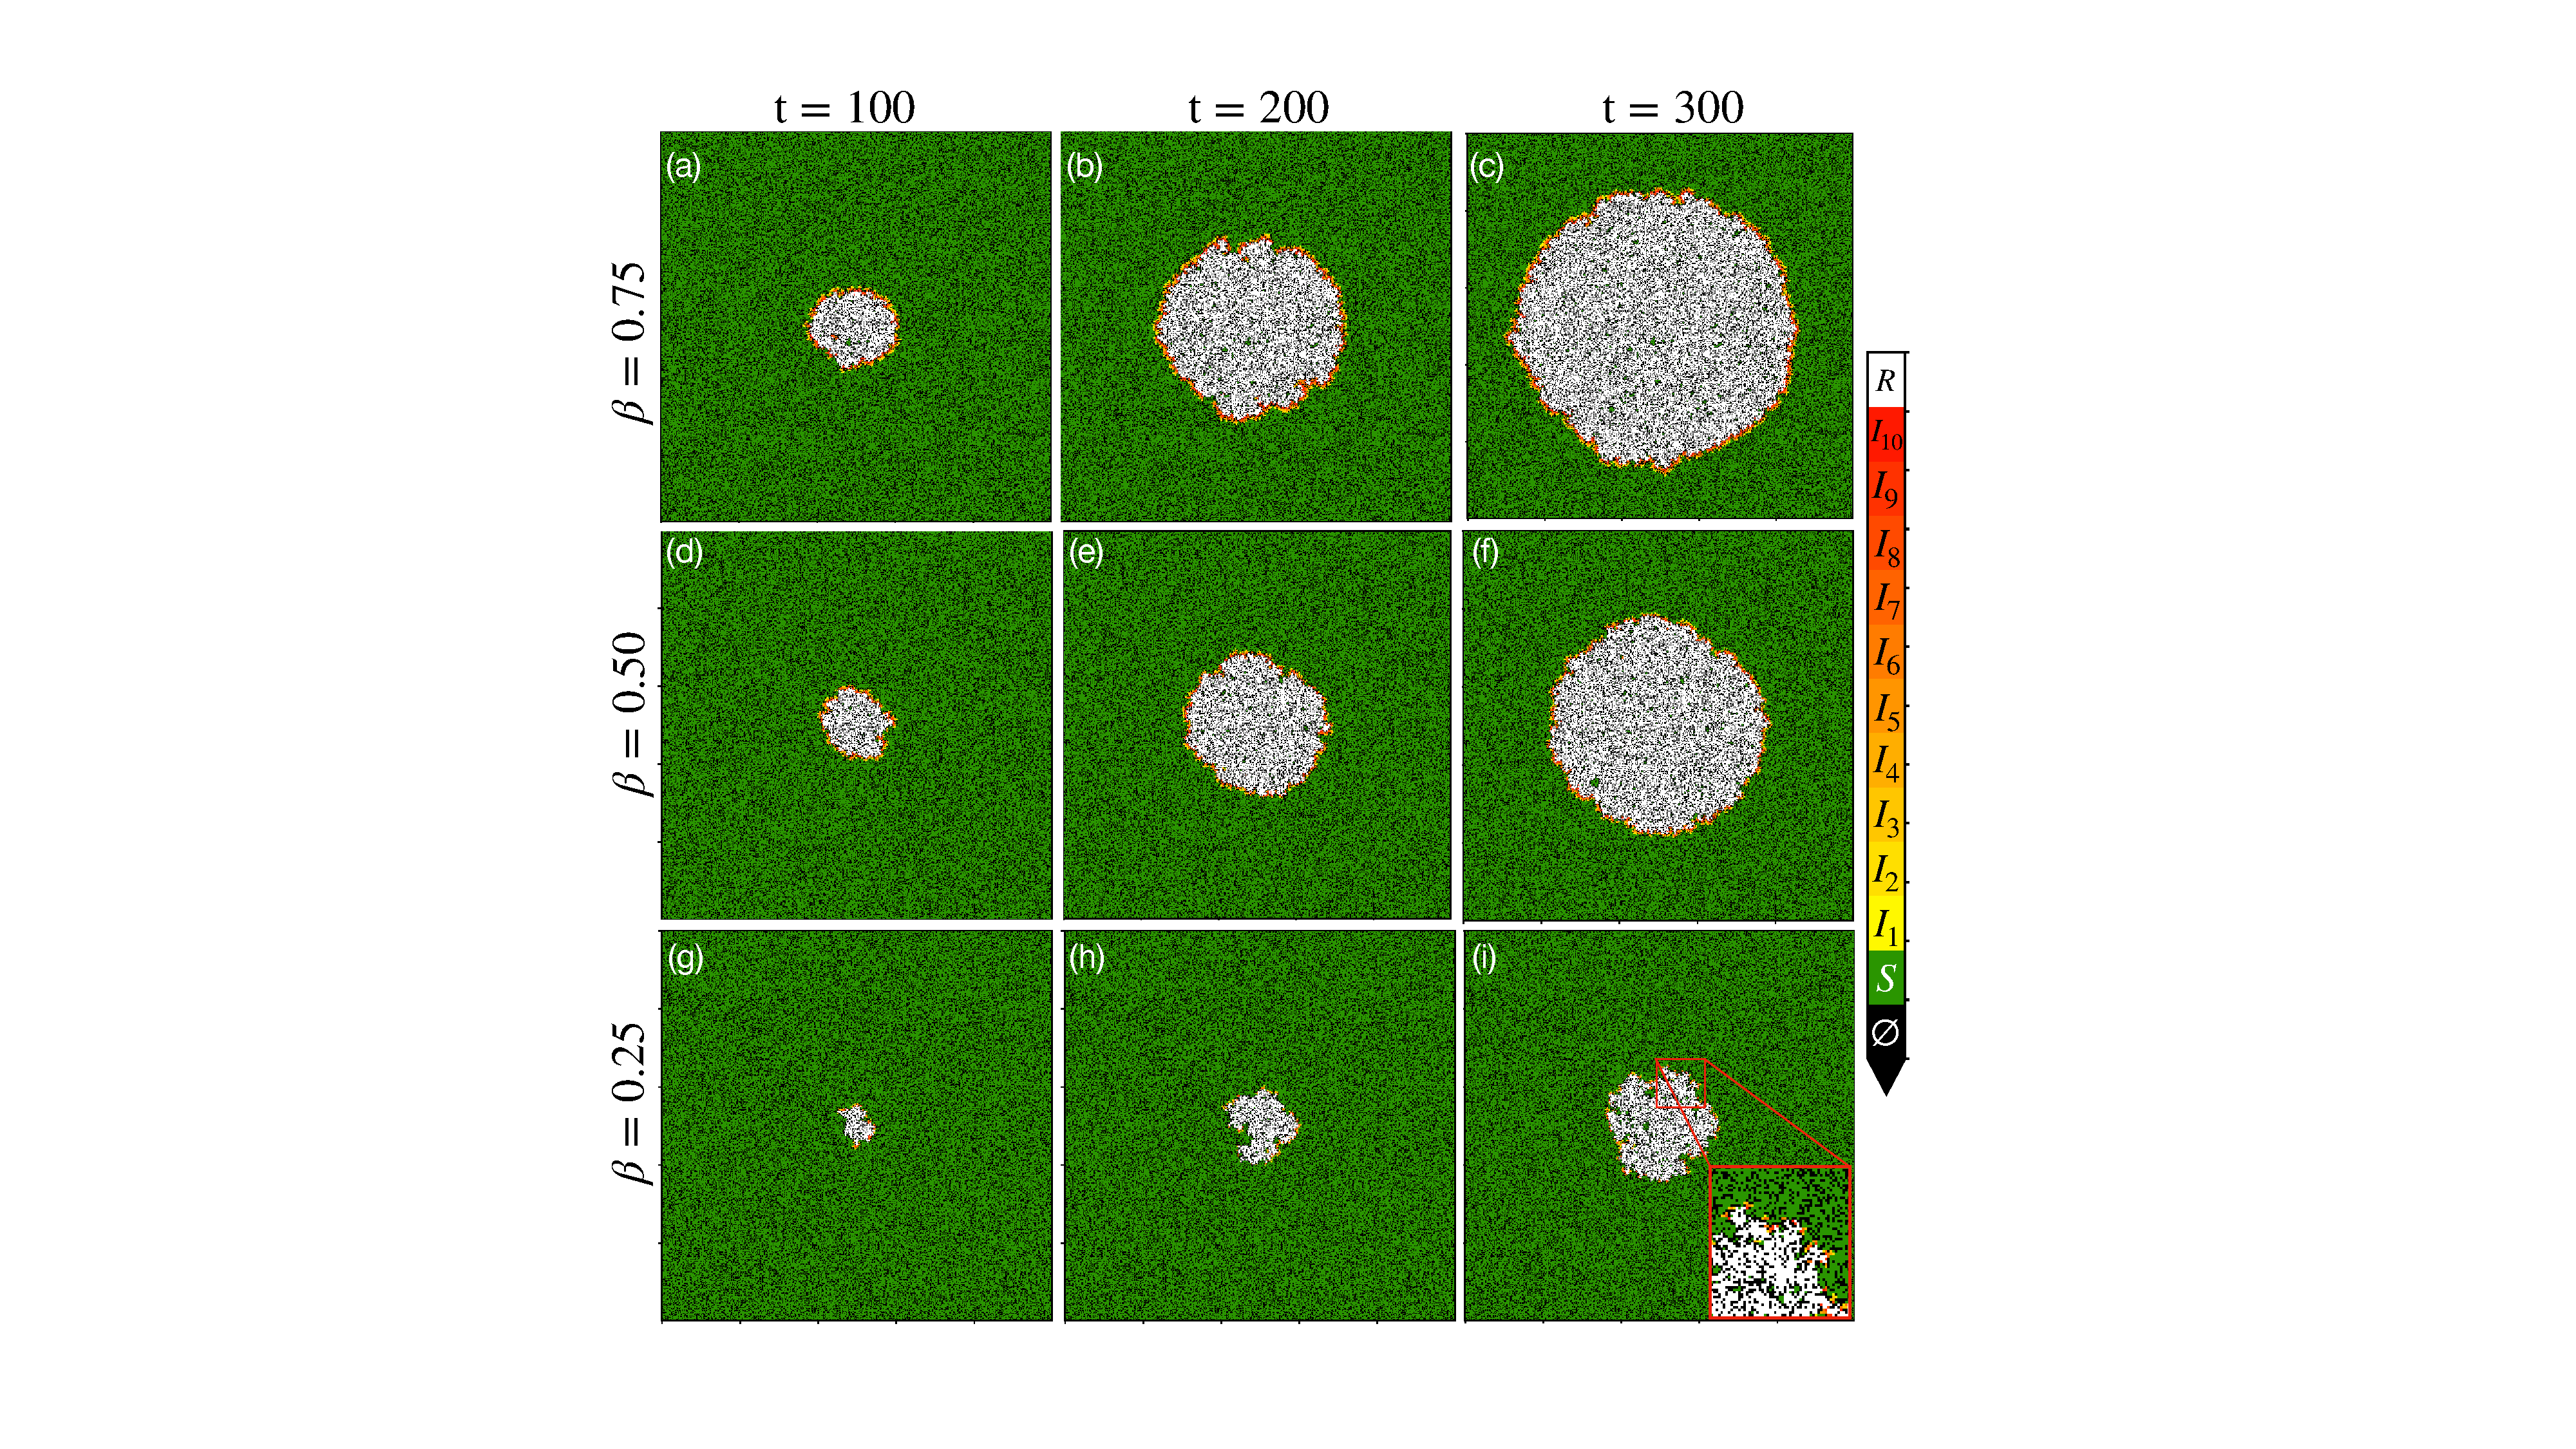
\includegraphics[scale=0.45]{chapter3/figures/figure3-two-param-model.pdf}
    \caption{Introducing an infectivity parameter $\beta$. The SLM is shown running on a domain of size $500\times500$ for fixed $T=10$ and density $\rho=0.70$. Simulation reveal that $\beta$ has an impact on the wave-front speed and changes the percolation threshold.}
    \label{fig:slm}
\end{figure}

\begin{figure}
    \centering
    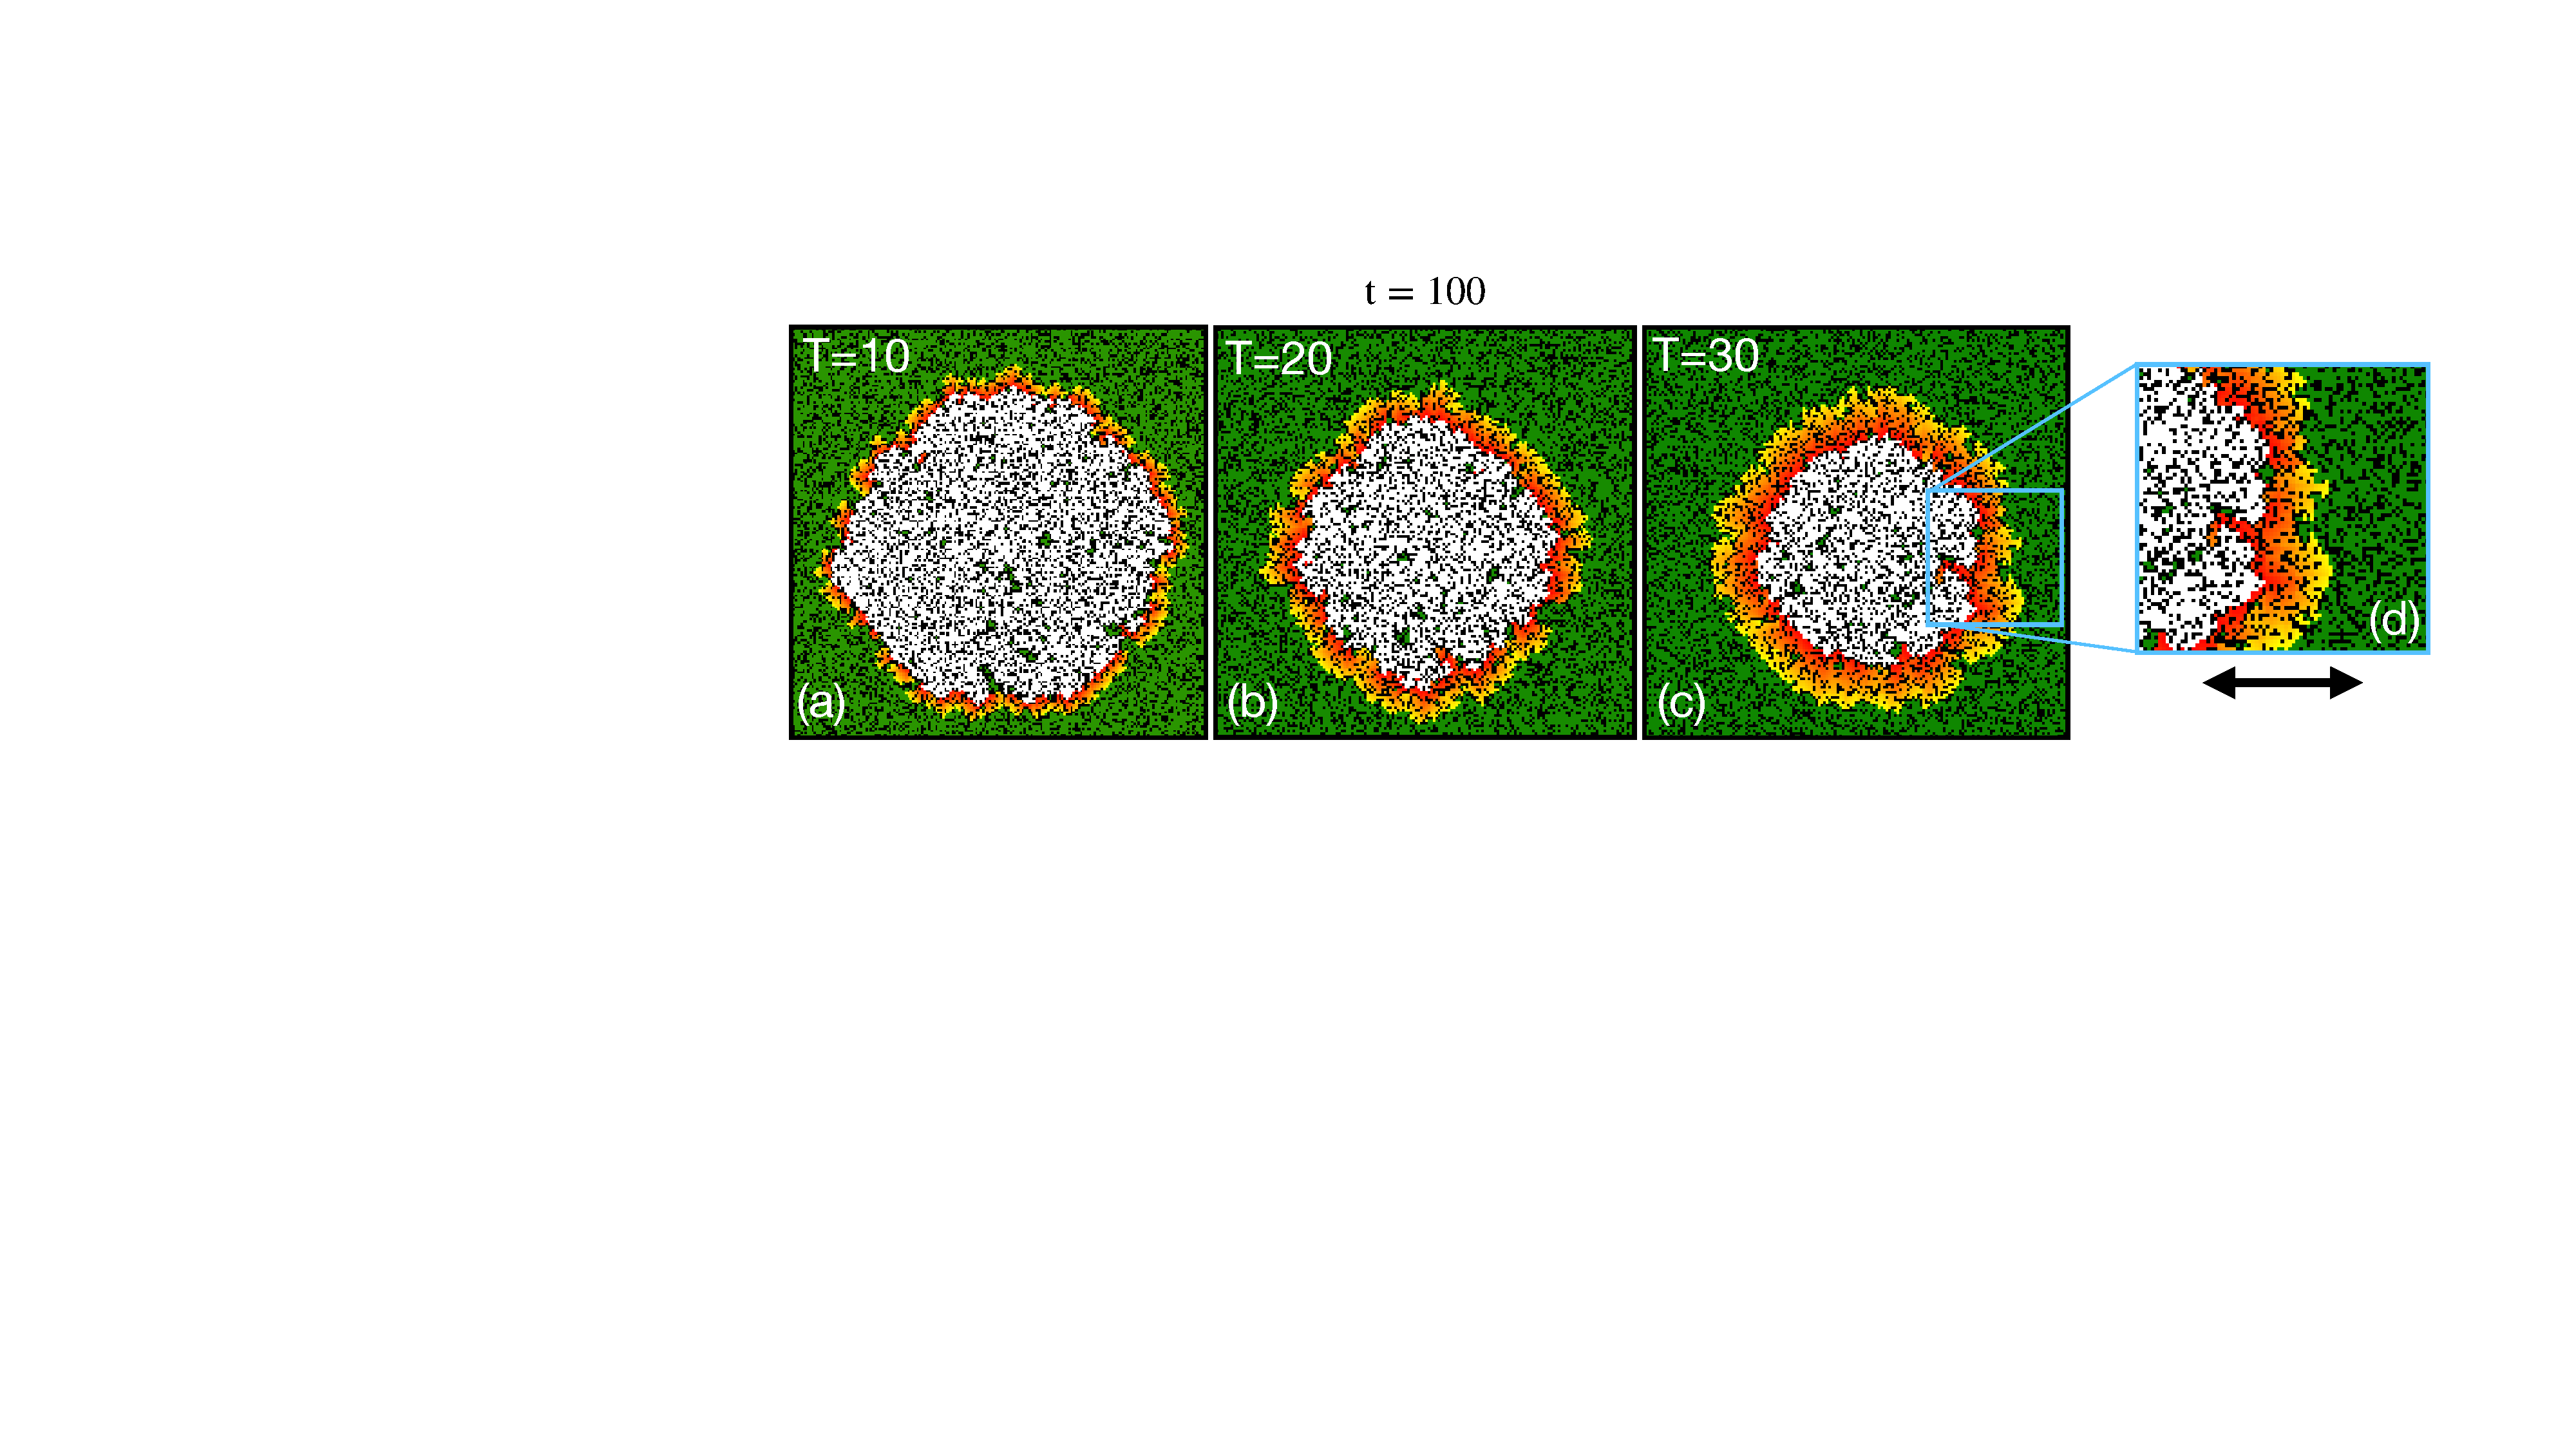
\includegraphics[scale=0.35]{chapter3/figures/figure5_.pdf}
    \caption{Simulations through a single time-step for fixed density and infectivity reveal that $T$ has little impact on the speed of the wave-front. 
    However, increasing $T$ leads to a thicker wavefront, as the posterior interface (between $R$ and $I$) lags behind the evolving wave-front (between $S$ and $I$).}
    \label{fig:slm-wave-front}
\end{figure}

\newpage

\section{Epidemic thresholds}
\label{sec:SLM-epidemic-threshold}

Previously in section \ref{section:universality}, the percolation probability was examined over one parameter of host density.
A threshold occurred over a narrow range of densities and separated the regime of epidemic and pathogen extinction.
Notwithstanding, we did not examine the rate of pathogen propagation nor any additional dynamic information.
In order to capture spreading rates, a metric comprising the `spreading velocity' is introduced, captured by: 
\begin{equation}
\label{eq:vel_eff_r}
    v_{radial(t)}=\sqrt{N_I(t+1)-N_I(t)}
\end{equation} 
where, $N_I$ is the number of infected trees in the domain at time-step $t$. 
The difference in $N_I$ between time-steps gives an `effective' radial velocity. %
The number of spatial units progressed by the pathogen is averaged over all angles per unit time. %
Strictly speaking, Equation (\ref{eq:vel_eff_r}) is valid only for $\rho > \rho_c$; at the percolation threshold, the wave-front assumes a fractal dimension and averaging over two dimensions becomes unreasonable.

The time-series, $v_{radial}(t)$ is shown in Figure \ref{fig:vel_eff_rad_metric}(a) for three combinations of $(\rho, \beta)$.
Unsurprisingly, higher-valued combinations produce a higher velocity.
Additionally, initial instability is most significant through the first $\sim 200$ time-steps, a consequence of the initial conditions which suggests the system has yet to reach a steady state.
Here, the system is said to be in a transient state.
In Figure \ref{fig:vel_eff_rad_metric}(a), a simulation average $\overline{v}_{radial}(t)$, 
can be determined and plotted as a horizontal line, repeating the measurement multiple times over an `ensemble', gives a probability distribution. 

Figures \ref{fig:vel_eff_rad_metric}(b-d) display the probability density functions\footnote{
To reduce artefacts of initial transience, any simulation that became extinct before the initial transient period 
of $t_{tr}\approx 200$, was excluded from calculations of the ensemble mean.} of the mean velocities.
In all panels, the vertical black line inside each distribution depicts the ensemble mean velocity.
For higher host densities, the mean velocity increases and distributions appear somewhat narrower.
Additionally, Figures \ref{fig:vel_eff_rad_metric}(b-d) suggest that $\beta$ plays a role in determining the velocity variance, as the distributions become wider with lower infectivity, cf. the green and blue distributions.

For now, the important statistic is merely the ensemble mean, denoted by $\big\langle\overline{v}\big\rangle$.
although, from Figures \ref{fig:vel_eff_rad_metric}(b-d), we can begin to access the third-order statistical moment of skew.
Namely, the green distributions become progressively right-skewed as density is lowered.
Statistical measures over the ensemble have exciting applications and can detect an early warning signal, a topic covered in the next chapter.

\begin{figure}
    \centering
    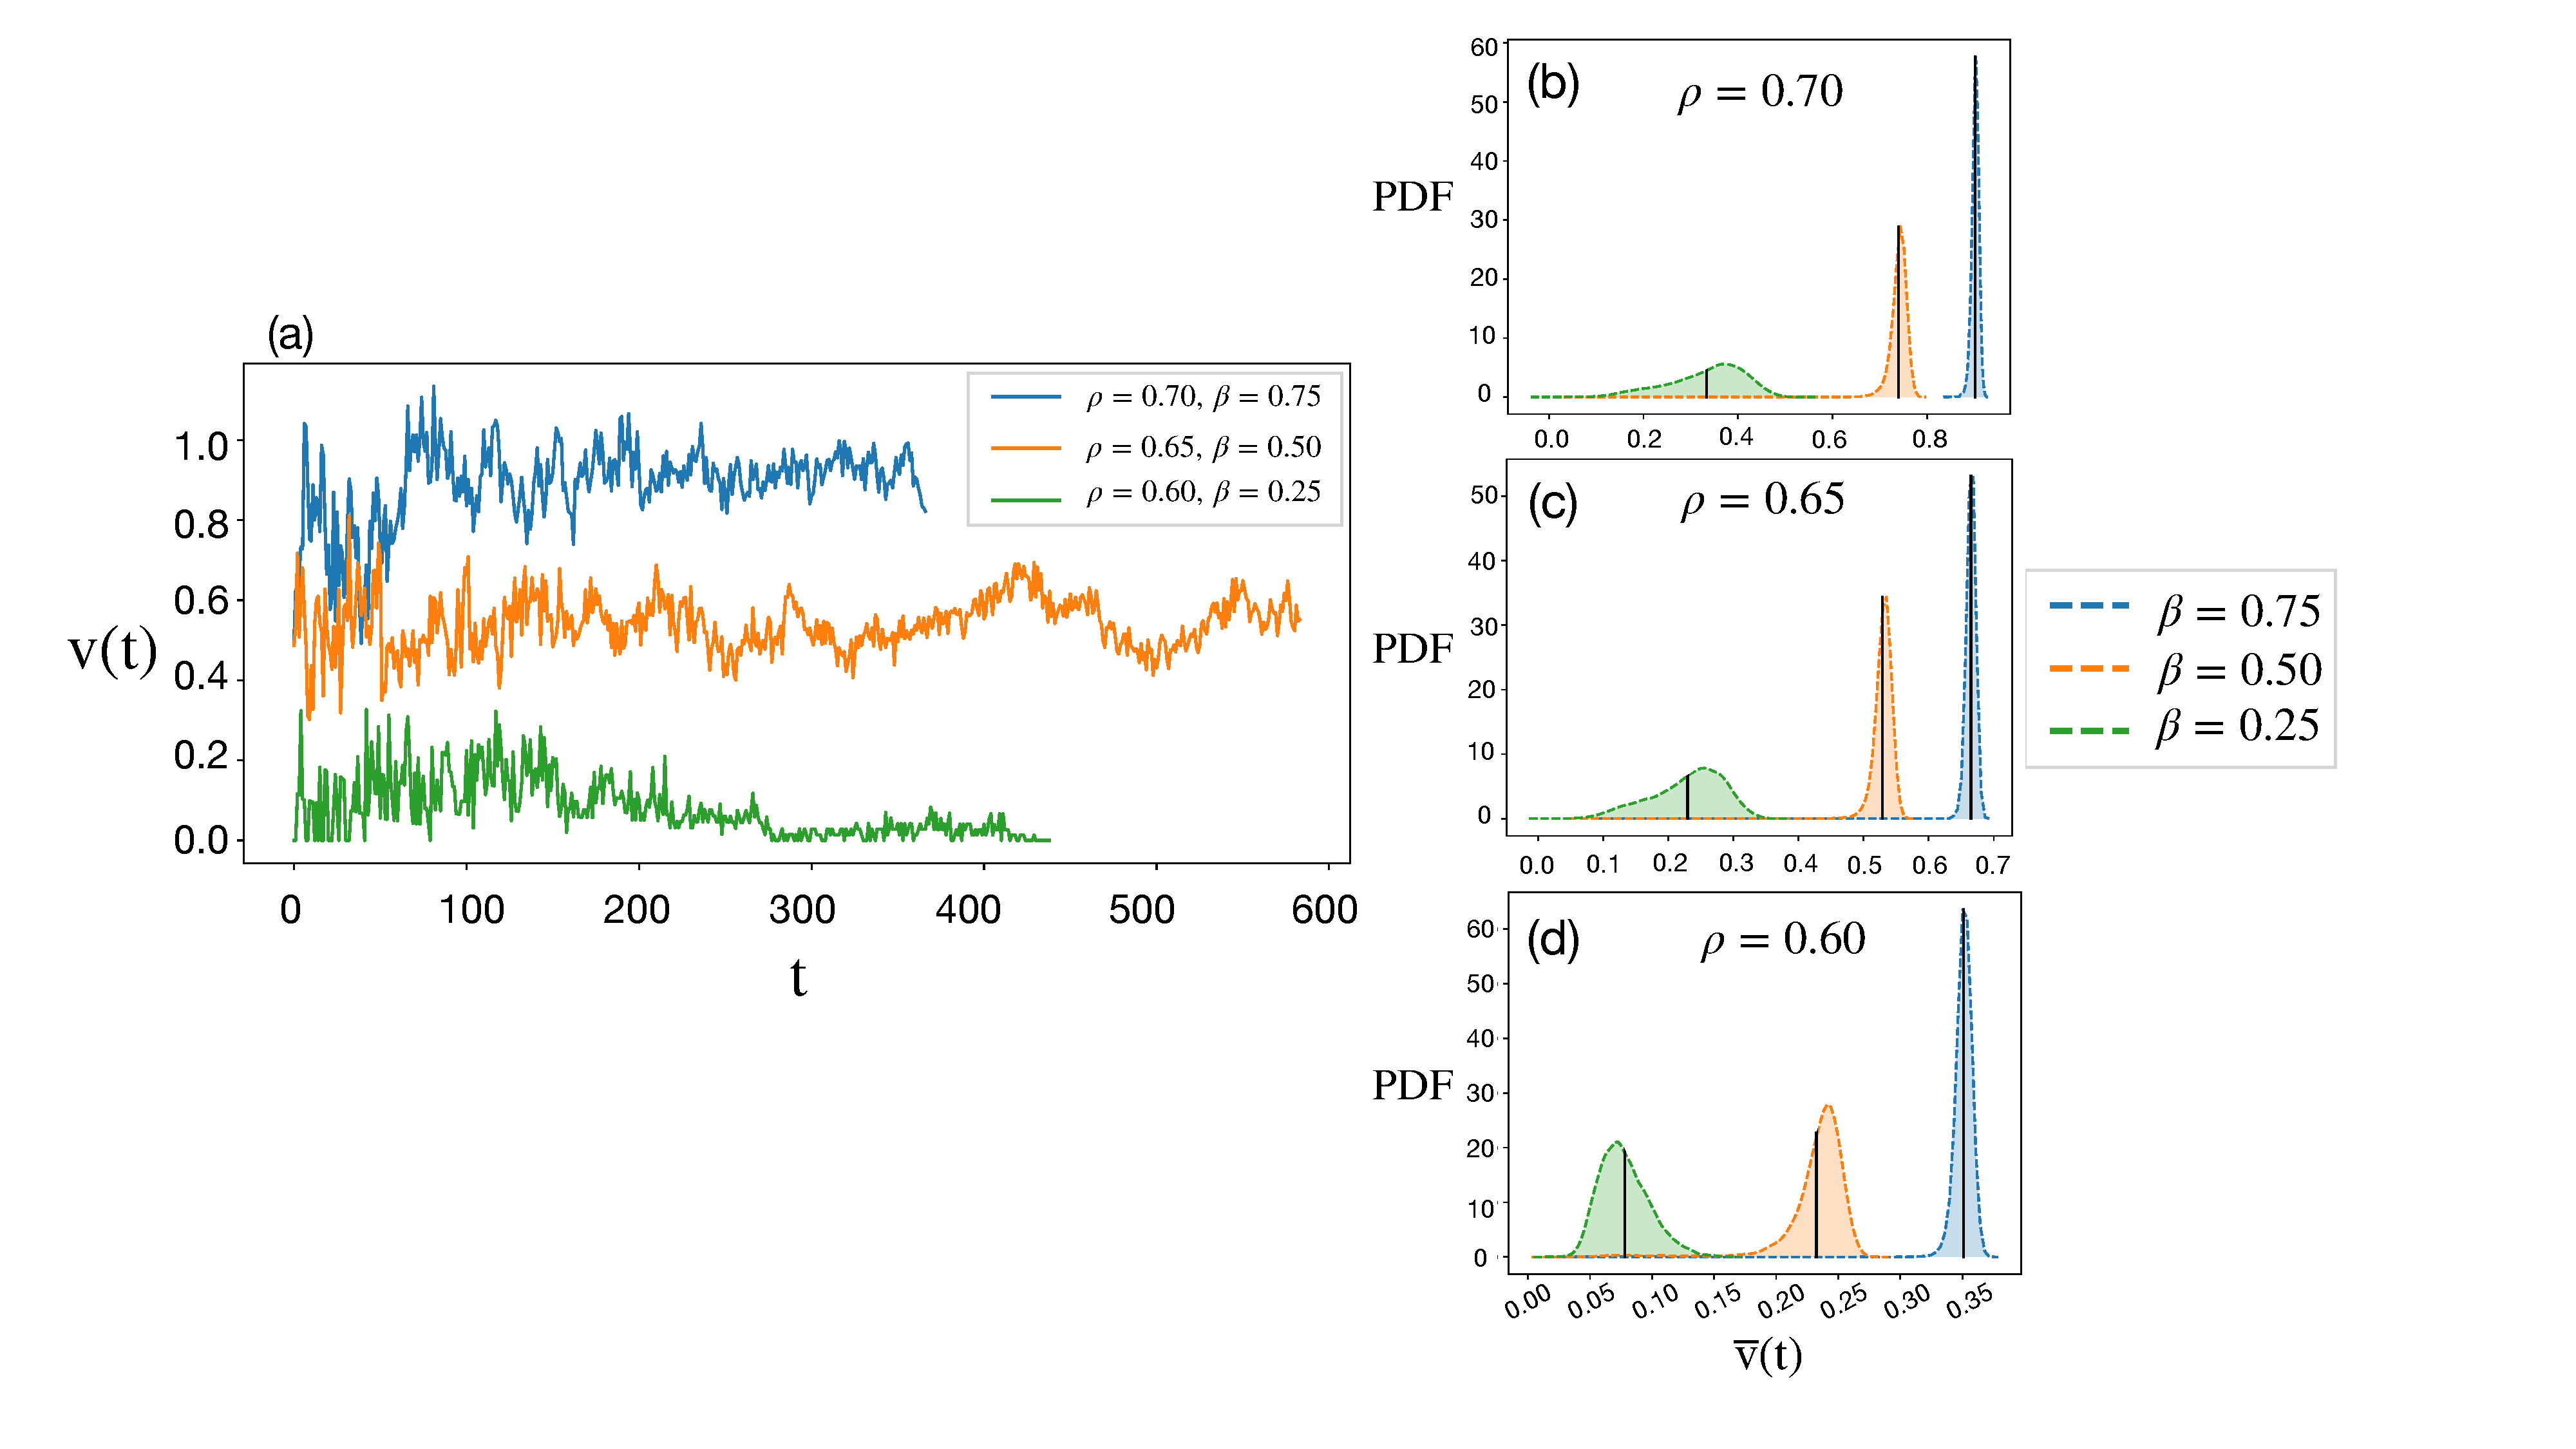
\includegraphics[scale=0.26]{chapter3/figures/figure7.pdf}
    \caption{(a) The velocity metric time-series $v_{radial}(t)$ is shown for three typical simulations, higher values of $\rho$ and $\beta$ give higher mean values of propagation speed. (b-d) The probability density function of mean spreading velocity $\big\langle \overline{v}_{radial}(t) \big\rangle$ for variations in $\rho$ and $\beta$.}
    \label{fig:vel_eff_rad_metric}
\end{figure}

Figure \ref{fig:slm_pspace} contrasts the epidemic threshold according to both percolation and velocity-based metrics.
In Figure \ref{fig:slm_pspace}(a), a one-dimensional line through the parameter-space of $\rho$ reveals the percolation probability for the three different infectivity parameters shown.
The vertical dashed line shows the accepted percolation threshold, $\rho_c$, for a two-dimensional square lattice. 
For $\beta \in [0.50, 0.75]$, the probability of percolation is identical to that shown in Figure \ref{fig:ch3-perc-pr};
However, a lower value of $\beta = 0.25$ decreases the percolation threshold, as evidenced by the green line shifting to the right.
Figure \ref{fig:ch3-perc-pr}(a) intuitively demonstrates that a pathogen with a low value of infectivity requires a more significant tree density to spread.

The ensemble-averaged radial velocity $\big\langle \overline{v} \big\rangle$ (as per Equation \ref{eq:vel_eff_r}) mirrors the percolation threshold,
notwithstanding with some differences.
In Figure \ref{fig:slm_pspace}(b), we witness a significant increase in the propagation speed when the density crosses the threshold density $\rho_c$, 
notably for $\beta=0.75$ and $\beta=0.50$ shown in blue and orange. 
In addition, a higher $\beta$-value predictably yields a higher radial velocity, both before and after the epidemic transition.

Interesting behaviour is discerned by the contrasting the green curves (when $\beta=0.25$) in Figures \ref{fig:slm_pspace}(a-b);
the vertical dashed green line in Figures \ref{fig:slm_pspace}(a-b) highlight when epidemics begin to propagate to the domain edge reliably.
Therefore, when $\beta=0.25$ the velocity remains close to zero, yet the percolation probability is high. 
This observation indicates a regime of persistence in the model, where epidemics can survive for long periods, barely above the threshold \cite{gilligan2008epidemiological}.

The equivalent two-dimensional plots over the full parameter-space of $\rho$ and $\beta$ are shown in Figures \ref{fig:slm_pspace}(c-d) for percolation and radial-velocity respectively. 
The two-dimensional percolation probability depicts an abrupt transition between two stable regimes of extinction and epidemic, where
a narrow range of critical parameters $\rho_c$ and $\beta_c$ separate epidemic and extinction.
In contrast, Figure \ref{fig:slm_pspace}(d) shows the ensemble-averaged velocity that describes a smoother transition between states.
Therefore, one might argue that percolation captures the threshold with greater clarity as the distinction between epidemic states is more apparent.

One significant difference between the percolation and velocity-based metrics is that percolation depends trivially on infectivity beyond $\beta \approx 0.40$;
meanwhile, the radial velocity tends to increases for higher infectivities.
Between $0.15 <\beta<0.30$, a higher value of $\rho$ is needed for percolation to occur;
the equivalent velocity-based behaviour can also be seen, albeit with a more continuous transition.
A higher infectious lifetime $T$ lowers $\beta_c$, as more infectious time-steps increase the chance of secondary infections, thus lowering the threshold.
Here, the parameter-sweeps can be understood to portray an `\textit{epidemic phase diagram}'.

\begin{figure}
    \centering
    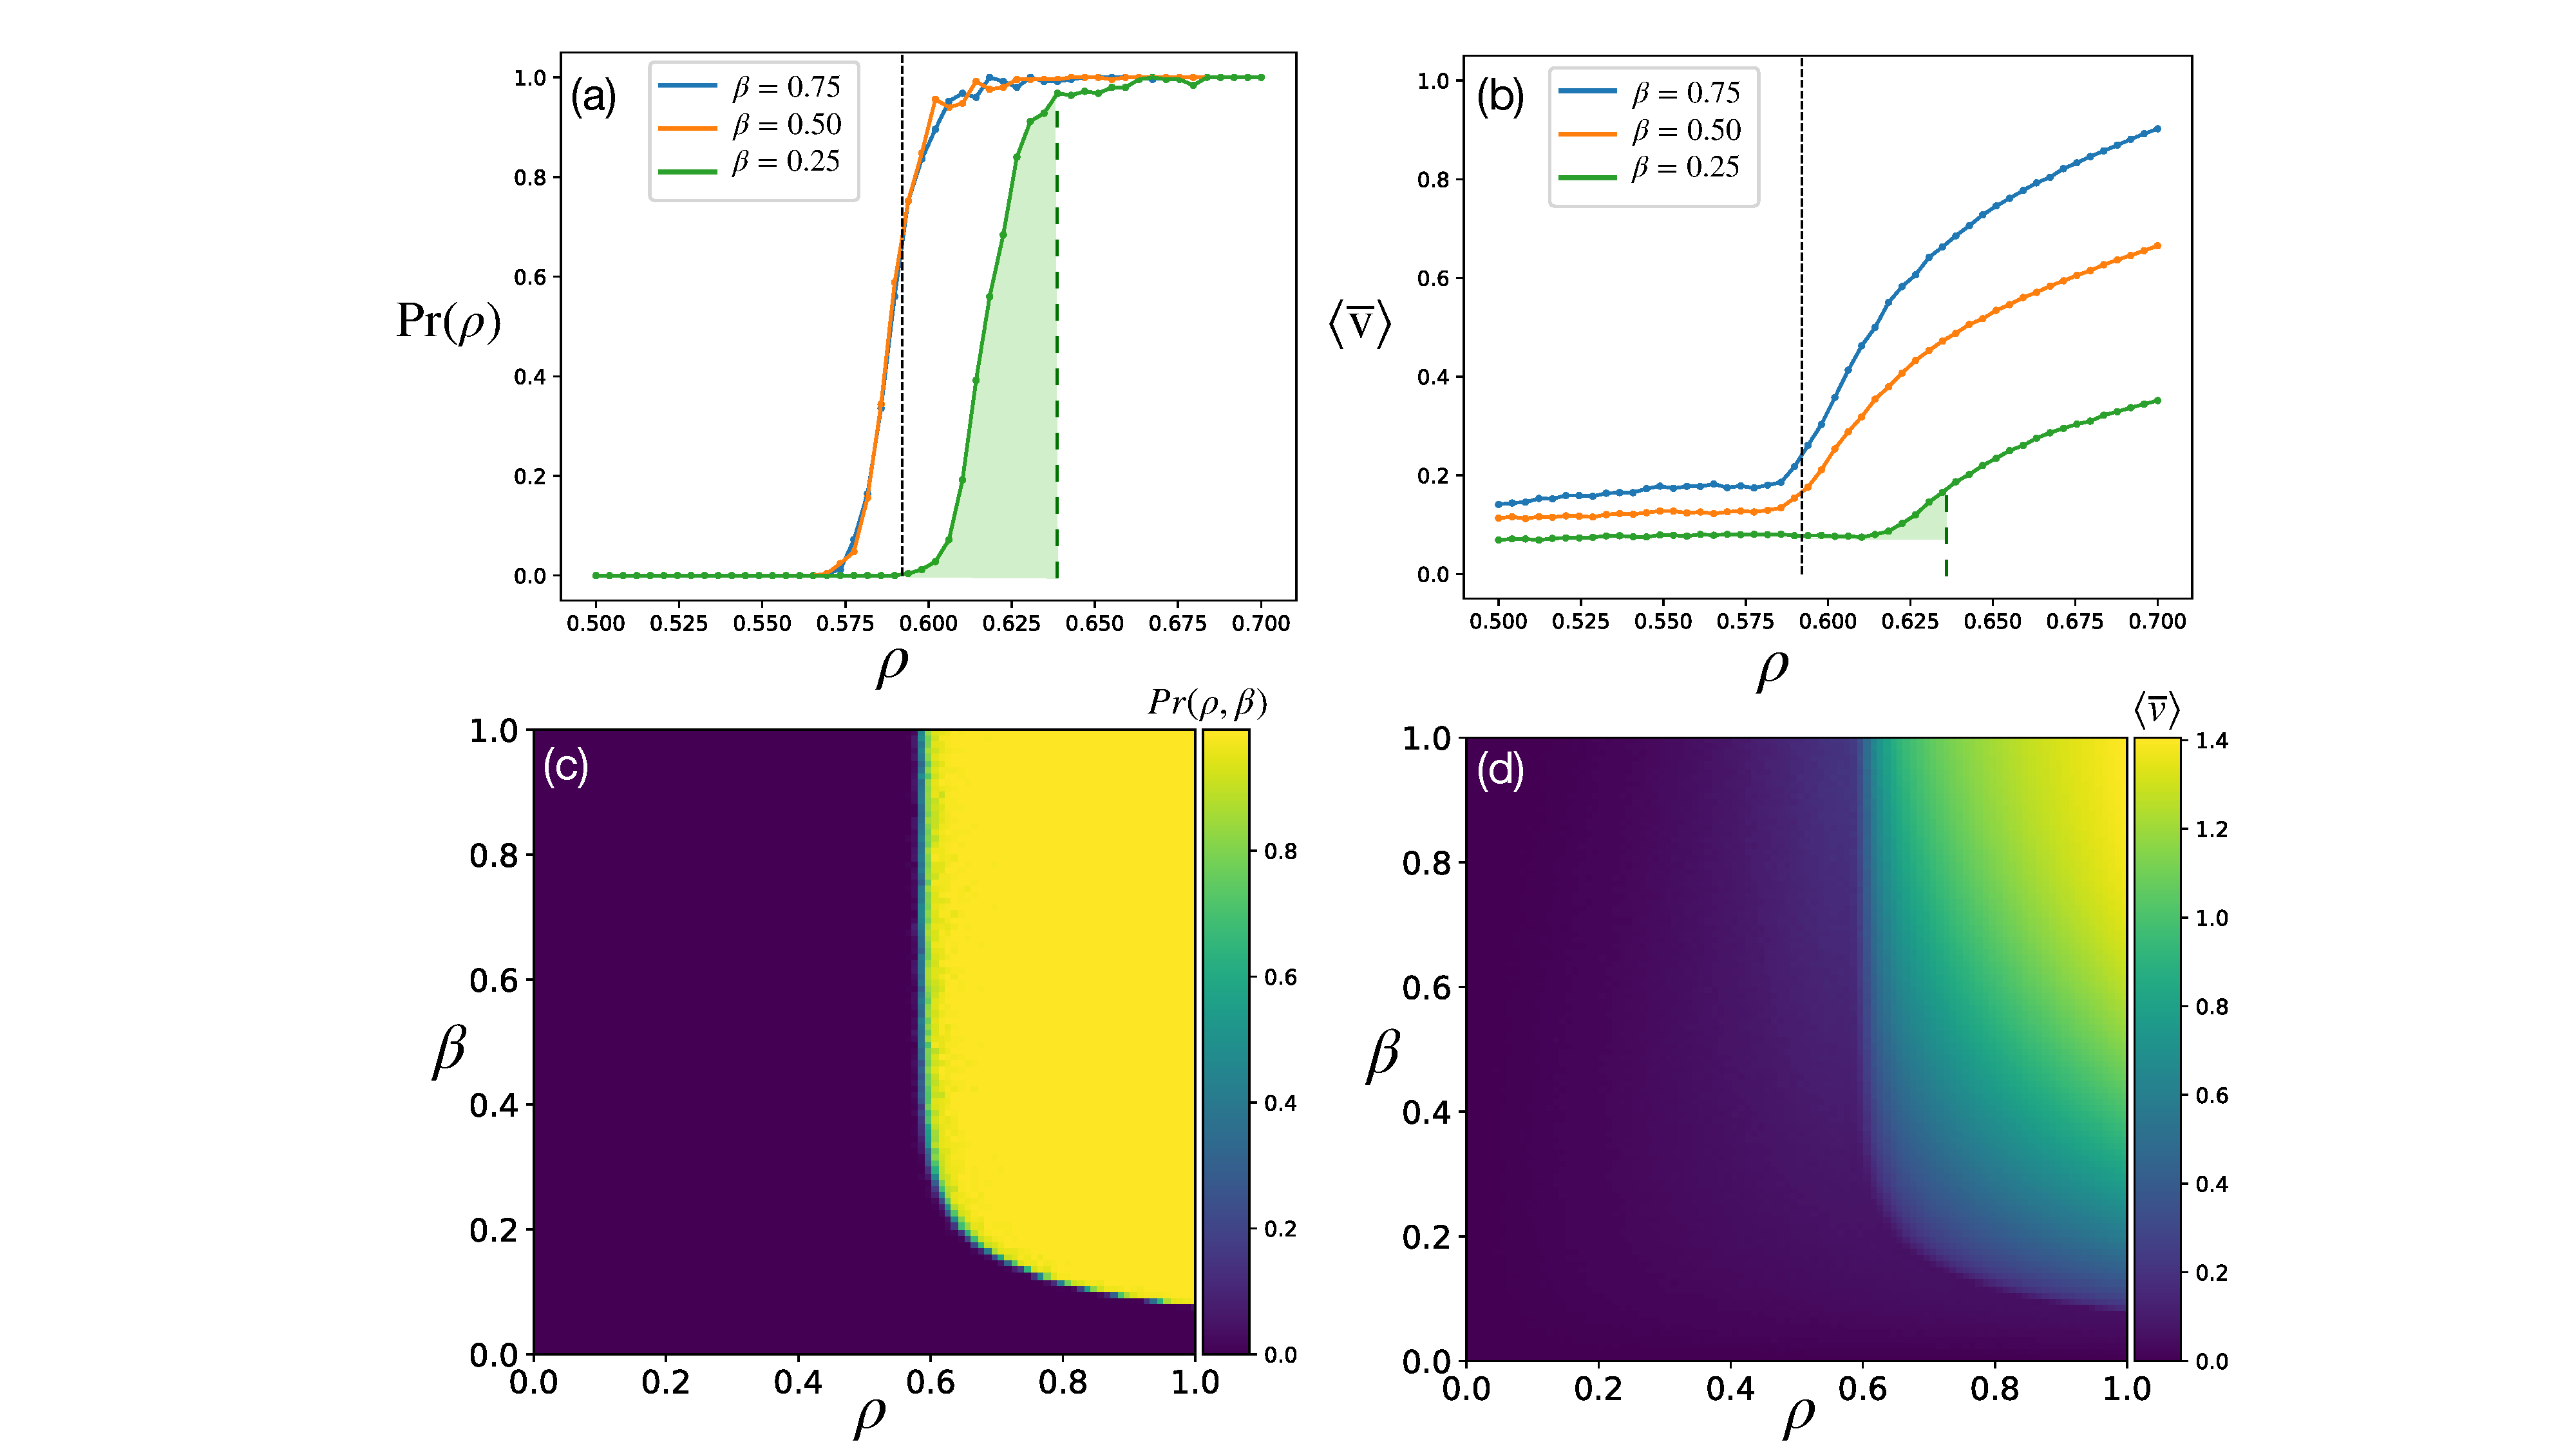
\includegraphics[scale=0.325]{chapter3/figures/figure4-perc-vel-phase-trans.pdf}
    \caption{
    A parameter sweep of $\rho$ and $\beta$ over the $500\times500$ domain. (a-b) The percolation probability is shown alongside the radial velocity over a one-dimensional parameter-space of $\rho$. For the lower-valued infectivity of $\beta=0.25$, the density threshold is slightly higher than classical percolation  $\rho_c=0.592$, indicated by the vertical dashed line. A gradual increase occurs when using the radial velocity, whereas percolation shows an abrupt transition. (c-d) A two-dimensional parameter sweep paints a similar picture.
    }
    \label{fig:slm_pspace}
\end{figure}

\newpage

\section{Chapter Summary}

This chapter introduced percolation theory, leading to a one-parameter percolation $SIR$ model of tree disease spreading through a forest.
The one-parameter model demonstrated stochasticity on account of the randomly populated host distribution inside a square lattice. 
Assessing the model on one lattice configuration signifies a limitation in our analysis; 
more rigorous treatments might consider examining the spread of disease on alternate lattices.
However, although only one lattice was employed, universal properties of the model would be expected to remain the same\textemdash such as the critical exponent describing the correlation length $\xi$\textemdash as discussed in section \ref{section:universality}.

In section \ref{ch3:two-param-model}, an infectivity parameter ($\beta$) was included in the model.
The infectivity parameter introduced temporal stochasticity into the system, as infections spread probabilistically between nearest neighbours \textemdash
as opposed to the one-parameter model that spreads between hosts with a probability of one.
The infectivity parameter altered the critical density; 
higher values of $\beta$ recovered the standard percolation threshold for a two-dimensional square lattice ($\rho_c\approx 0.592$), 
while lower values of $\beta$ increased the critical density required to support an epidemic.

In nature, a pathogen might interact with diverse hosts over various environmental conditions;
a relevant and interesting example includes the algae-like oomycete \textit{Phytophthora ramorum} (\textit{P. ramorum}). 
The pathogen \textit{P. ramorum} affects a wide host range \cite{GRUNWALD2012131}, 
including Larches (deciduous conifers of the genus \textit{Larix}) and southern beech (\textit{Nothofagus}), 
and some non-native oaks such as red oak (\textit{Quercus rubra}) \cite{grunwald2008phytophthora}.
Although, different genetic variants of \textit{P. ramorum} affect different hosts with varying severities.
For example, north American oak speceis are highly suceptible to the NA1 lineage \cite{rizzo2002phytophthora}, 
while UK larch trees appear highly suceptible to the European lineage EU1 \cite{king2015planta}. 
Therefore, the integration of $\beta$ in the SLM is undoubtedly simplistic and general; nevertheless, it permits a description of varying degrees of pathogen virulence.

Two metrics categorized the model's behaviour: the pathogens average radial velocity alongside a probability of percolation.
The percolation probability defined a sharper, more reliable transition between epidemic and pathogen extinction.
Although the percolation probability may prove more beneficial for classifying epidemic regimes, 
the radial velocity captured a similar threshold-like behaviour beside additional dynamic information in the form of a time series.
Subsequently, the time series was ensemble-averaged and examined over a sweep of $\rho$ and $\beta$ values. 

Interestingly, comparing the percolation probability to radial velocity revealed a parameter region above the threshold where the pathogen survives but slowly propagates to the domain boundary. 
This behaviour approximates persistence; the reader can find a review of invasion and persistence in section \ref{ch3:invasions_and_persistence}.
However, neglected host population dynamics in the SLM prevents long-term coexistence between host and pathogen, 
an essential requirement of persistence \cite{gilligan2008epidemiological}. 
Accordingly, the SLM only approximates invasion and persistence, which therefore signifies a limitation in the framework. 

As we look to construct a more representative model, it is worth remarking on the most significant assumptions that underpin the SLM:
\begin{enumerate}
    \item \textbf{Local NN interactions}: in reality, many dispersal mechanisms exist to propagate the spread of disease\textemdash 
    section \ref{ch2:dispersal} contains more information. 
    Undesirably, local interactions in the SLM revealed unnatural artefacts of lattice geometry.
    Moreover, as the pathogen could not jump over empty lattice sites, epidemics were only possible above the percolation threshold, 
    i.e. when connected clusters of hosts span the domain.  
    
    \item \textbf{Uniform dynamics:} in general, pathogen-host interactions transpire with varying degrees of severity; 
    for example, age-dependent severity in ash dieback and the species-level virulence of 
    \textit{P. ramorum}. 
    In contrast, the SLM considers that A) the transition probability into $R$ occurs with a uniform number of steps 
    B) the probability of transition into $I$ is identical between hosts 
    C) $\beta$ is simplistic, with no spatio-temporal (environmental) dependence. 
    More generally, we have constructed a general, abstract model with no specific pathogen in mind.
    
    \item \textbf{Host distribution}: natural tree populations present rich spatial structures with varying degrees of clustering and aggregation \cite{doi:10.1086/342823}.
    Indeed population clustering has been confirmed over various spatial, from the tree-level to the field-level \cite{wiegand2007analyzing}.
    Therefore, the flat randomly distributed host population considered in this chapter falls short of a realistic description.
    Moreover, the SLM describes the spread of disease in a densely populated forest, and as we look to model the spread of disease over Great Britain realistic tree canopy cover data should be incorporated into the framework.
\end{enumerate}
Despite the assumptions and simplicity of the SLM, it provides a general setting upon which to elaborate.
The next chapter outlines all the applications that were investigated using the SLM.
\newpage 

% 4) Application of the simple lattice model--moving to a realistic host landscape
% -----------------------------------------------------------------------------
% 1) Move to a map of the UK 
% 2) show edge effect and epicenter changes
% 3) introduce the data-set in a formal capacity + define the threshold function
% 4) show how heterogeneity changes the problem i.e. discontinuities in the phase diagram
% -----------------------------------------------------------------------------

\chapter{Simple lattice model: applications}
\label{chapter:SLM-applications}

Previously, a percolation-based $SIR$ model of tree disease spreading through a forest was outlined, named the simple lattice model (SLM).
The SLM provides a flexible foundation for generalising as we look to model the spread of disease over realistic landscapes focused in Great Britain.
This chapter aims to examine some applications of the SLM.
In particular, two applications divide the chapter, beginning with the early warning systems (EWS) for forest management and ending with a toy model of landscape-level spread.

Firstly, the system for EWS detection put forward by \cite{OROZCOFUENTES201912} is extended; the original publication considered one fixed parameter of $\beta$, here we generalise the analysis to the entire $\beta$ parameter space. In addition, we employ an alternative metric that permits a more precise EWS detection.
Secondly, the SLM will be adapted to construct a toy model of landscape-level epidemics in Great Britain.
More specifically, units of individual trees in the SLM are re-scaled to $\mathrm{1km \times 1km}$ patches 
and projected onto a predicted oak abundance data set given by \cite{hill.data}.
The toy model denotes the first step towards a more representative framework over realistic landscapes.

\section{Early warning signals}
\label{sec:EWS}

Applications of early warning signals have been investigated by \cite{OROZCOFUENTES201912} for forest management and ecosystems services.
The results focused on a one-dimensional parameter space of tree density $\rho$ over a square lattice with fixed infectivity $\beta$.
The study observed statistically significant changes (or signals) in the
moment-generating functions (of variance, skew and auto-correlation) for the radial velocity.
Changes in variance, skew or auto-correlation can preempt epidemic phase transitions, 
thus providing helpful information that could aid forest and plantation managers to maintain tree health. 
Here, we offer a small extension to some of the concepts presented by \cite{OROZCOFUENTES201912}.
In particular, a new domain and metric are used to detect more precise, early warning signals.  
The analysis is generalised to two dimensions in the parameter-space of $\rho$ and $\beta$. 
After introducing these alternative concepts, we discuss some of the problems and complexities encountered with ensemble-averaging. 

\subsection{Cylindrical geometry}

The metric used by \cite{OROZCOFUENTES201912} to quantify early warning signals had a similar form as Equation \ref{eq:vel_eff_r}, albeit with the inclusion of $N_R$.
That is, the results included both the infected and removed ($N_{I+R}$), whereas Equation \ref{eq:vel_eff_r} is based on just the infected ($N_I$). 
Unfortunately, the radial velocity (based on the number of infected and removed trees) can lead to confusing results, as geometrical effects alter the a rate of increase as the wave spreads outward; this is particularly visible for later times when the wavefront extent is considerable.\footnote{See Figure 4d in \cite{OROZCOFUENTES201912}, the apparent rate of increase in the velocity metric is purely due to geometry artefacts and the metric definition.}.
We will use an alternate lattice geometry to mitigate geometric effects.

Consider a rectangular domain of size $[L_x, L_y]$ where $L_x>L_y$ and $(x, y)$ represent dimensions of width and height respectively.
Figures \ref{fig:ews-primer}(a-c) shows the domain, henceforth referred to as the `channel' domain, over three time-steps for parameters above the threshold, $\rho=0.65$ and $\beta=0.50$.
The initial conditions are adjusted, so the first column (denoted by $x_0$, taken as the origin) is infected.
In addition, the boundary conditions permit the disease to propagate freely in the $+x$ and $\pm y$ directions, thus realising a cylindrical geometry with periodic boundary conditions in $y$ direction and fixed boundary conditions in $x$.

We register a percolation event in the channel domain if an infected tree reaches the last column, denoted by $x_m$
The percolation threshold shifts toward higher densities if the domain is sufficiently narrow (having a high aspect ratio), as the dimensionality of the travelling wave to somewhere between one and two dimensions\footnote{Additionally less space in computer memory is occupied and simulation time is lowered}. 
The higher percolation threshold can be explained by gradually increasing the domains aspect ratio;
in the limit $L_y = 1$ and $L_x  \gg 1$, a one-dimensional domain is realised, and the critical host density increases to $\rho_c=1$, i.e. the well-known one-dimensional percolation threshold.

As expected, studies have confirmed that site and bond percolation in two and three dimensions depend critically on a cylinders aspect ratio \cite{sangare2009continuum}.
Therefore, we choose an aspect ratio that approaches the percolation threshold for a two-dimensional square to keep consistent with the numerical results of chapter \ref{chapter:SLM}. 
In practice, a channel of size $(L_x, L_y) = (350, 50)$, was sufficient, as shown through Figures \ref{fig:ews-primer}(a-c). 

\newpage

\begin{figure}
    \centering
    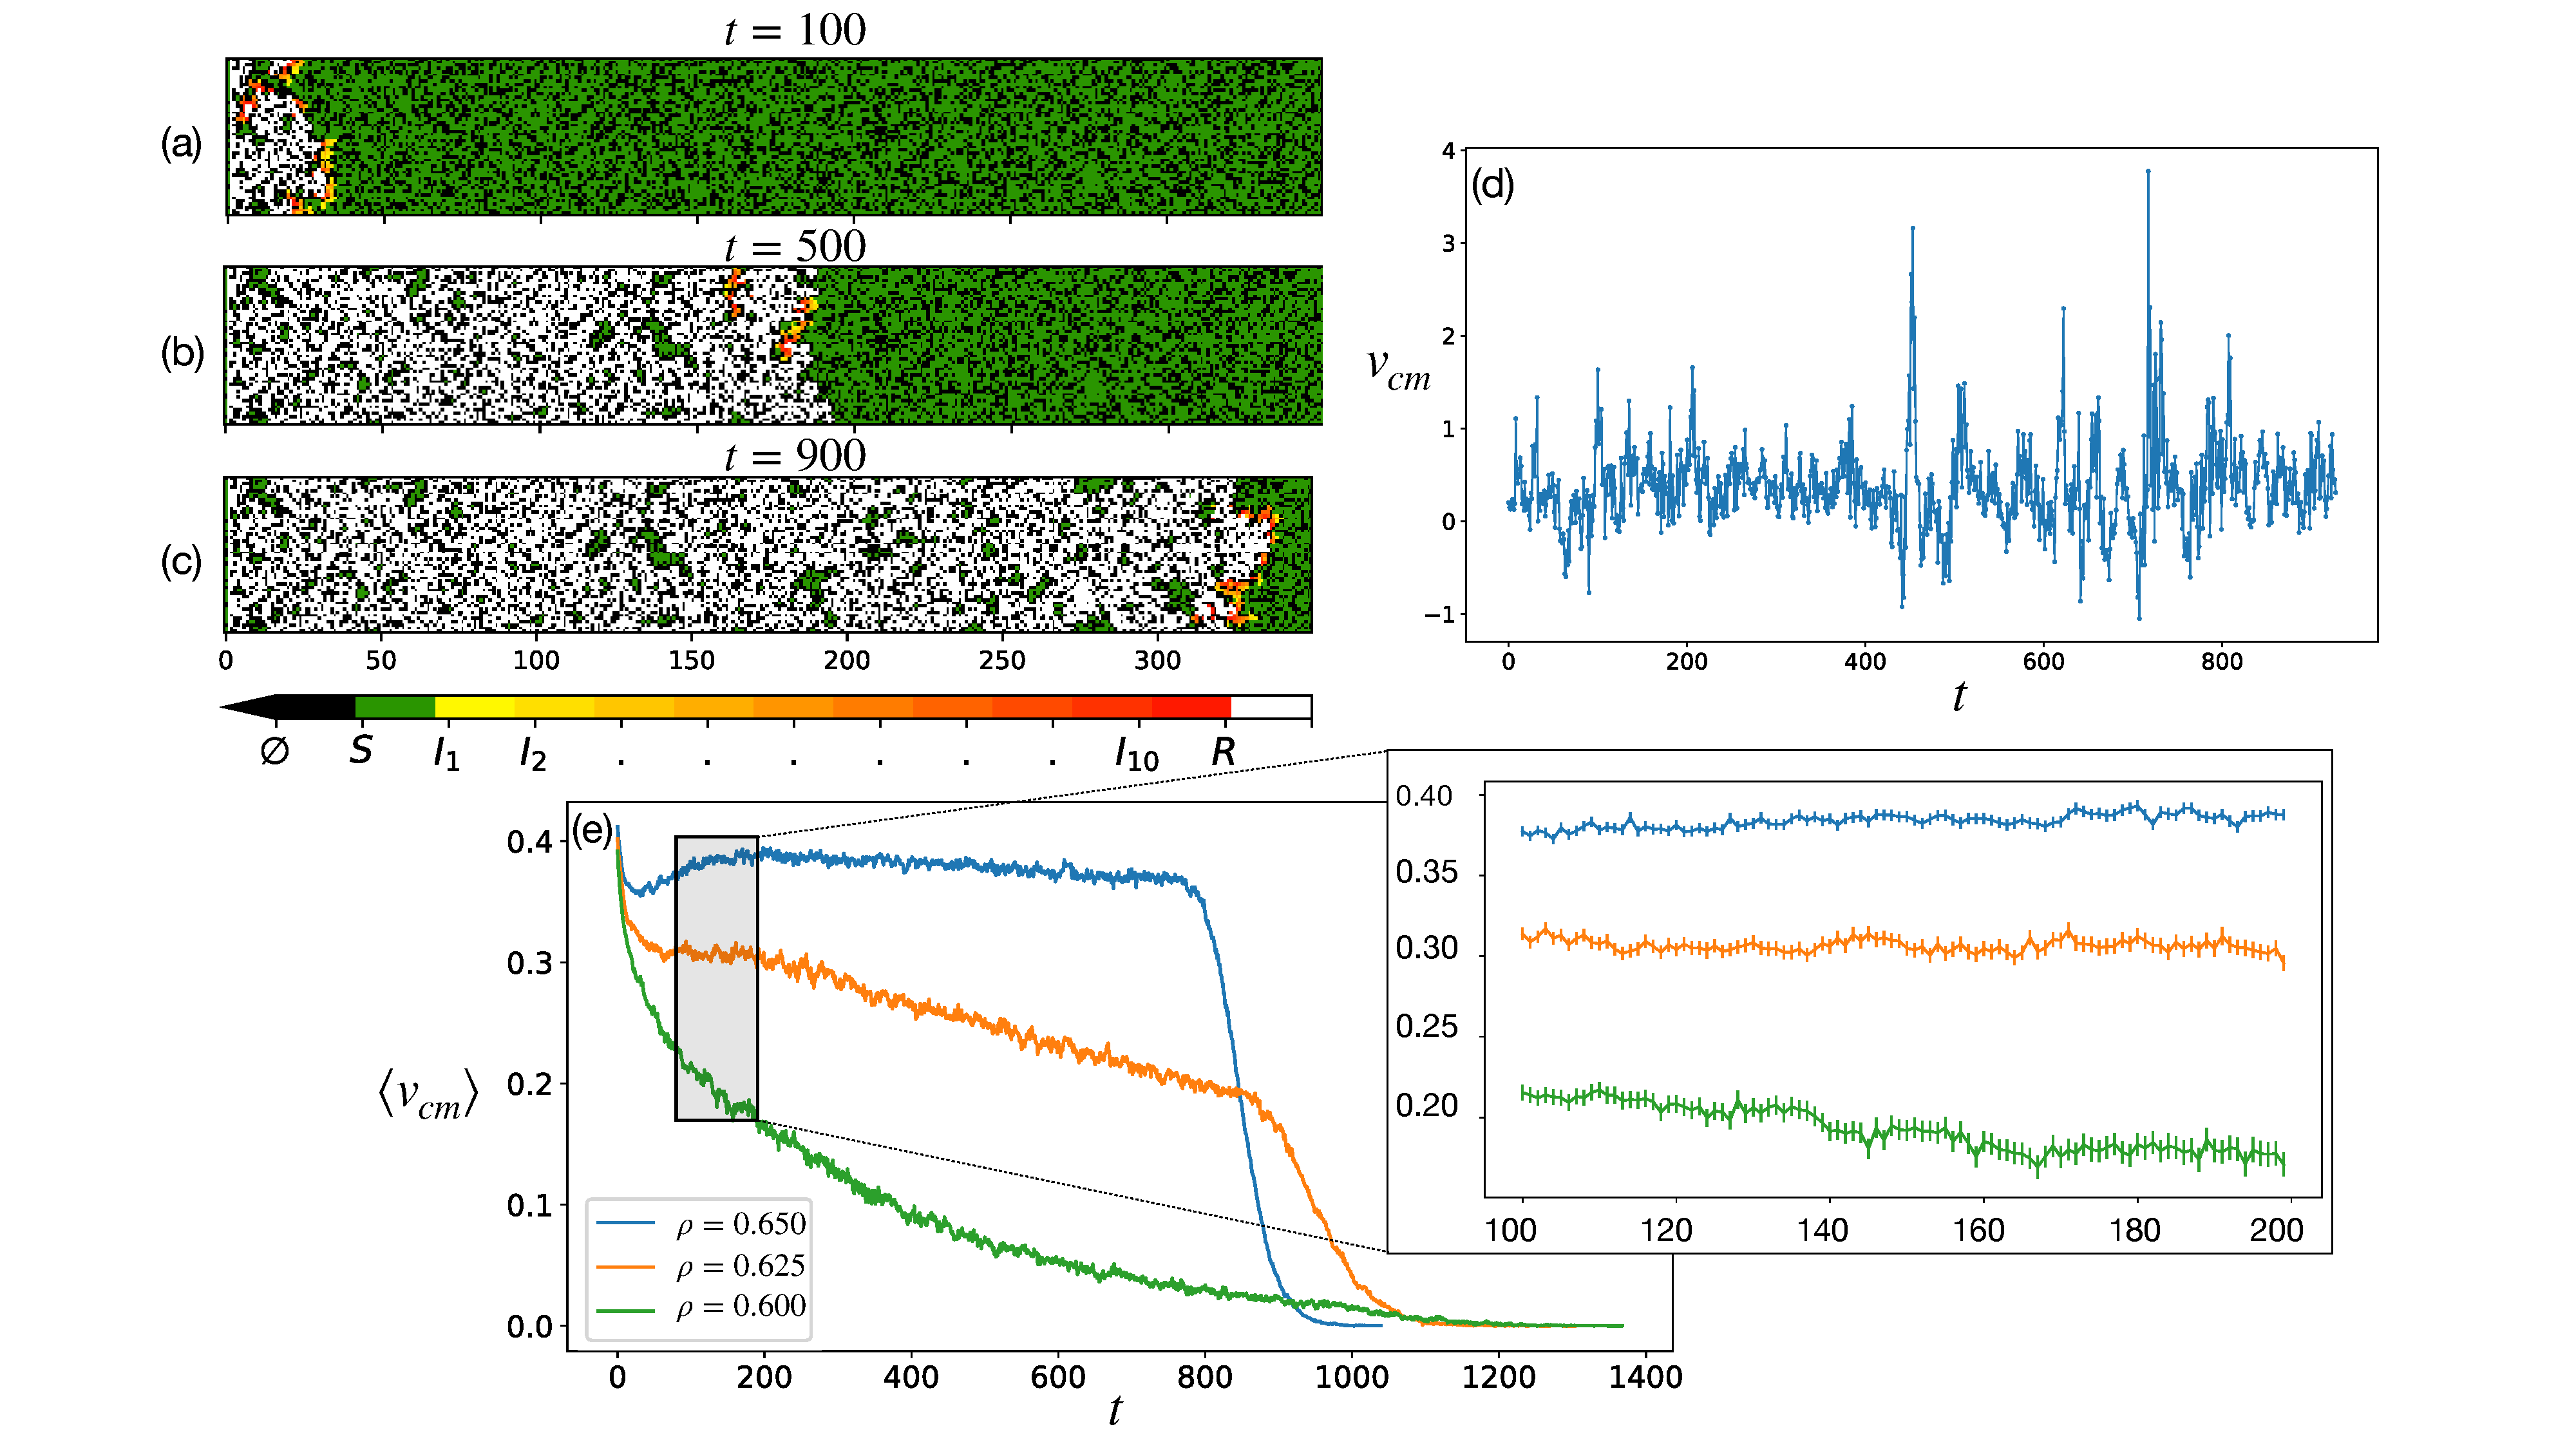
\includegraphics[scale=0.30]{chapter4/figures/figure1-channel-domain.pdf}
    \caption{
    (a-c) A channel domain of size $50\times350$ is shown over three time-steps for model parameters $\rho=0.65$ and $\beta=0.50$. 
    The center of infectious mass is recorded for each time-step. 
    (d) Plots of the center of mass time-series for the simulation illustrated in panels (a-c). 
    (e) The mean center of mass time-series (of $10^4$ repeats) for three variations in density and $\beta=0.50$. 
    Time-series begin to decay around the mean simulation run-time.  
    The zoomed inset shows the ensemble averaged time-series for $t\in[100, 200]$ and reveals increases in error bars lower density parameters.
    }
    \label{fig:ews-primer}
\end{figure}

\subsection{Centre of infectious mass}

The channel domain provides an advantageous setting to capture early warning signals, avoiding two-dimensional geometrical effects.
Moreover, the channel permits an improved (more intuitive) `centre of mass' metric (COM), based on the mean infectious tree displacement from the origin:
\begin{equation}
   v_{cm}(t) = \frac{\sum^i x_i(t)}{N_I(t)} - \frac{\sum^i x_i(t-1)}{N_I(t-1)}
   \label{eq:COM}
\end{equation}
where $x_i(t)$ is the spatial location along the $x$ axis of the $ith$ infected tree at 
time $t$ and $N_I(t)$ is the total number of infected trees at time-step $t$. 
 The form of Equation \ref{eq:COM} displays intrinsic similarities to the Newtonian center of mass:
 \[x_{cm} = \frac{\sum^i x_i\times m_i}{\sum_i m_i}\]
(where $m_i=1$ and $\sum^im_i= N_I$ in Equation \ref{eq:COM}).
Subsequently, the COM velocity will denote the metric defined by Equation \ref{eq:COM}. 
Figure \ref{fig:ews-primer}(b) depicts the COM time-series corresponding to the simulation shown in Figure \ref{fig:ews-primer}(a). 
The COM time-series allows for negative values and looks different to those shown previously in Figure \ref{fig:vel_eff_rad_metric}(a).

Figure \ref{fig:ews-primer}(c) illustrates the COM ensemble-average, denoted by $\langle v_{cm}\rangle$, for the three values of tree density.
On average, the mean time series begins to decay after the mean lifetime of the simulation; the blue time-series shows a drastic decrease around $t \in [800, 900]$, which coincides with the pathogen reaching the domain boundary\textemdash also reflected in Figure \ref{fig:ews-primer}(c).
The green time series lies just above the threshold for percolation, and it decays more gradually $t=0$ because of the higher pathogen extinction probability. 
A small number of long-lasting simulations with run times (exceeding $t>1000$ steps) occurred in the green time-series, indicating criticality in the system\textemdash 
previously likened to a regime of persistence in section \ref{sec:SLM-epidemic-threshold}.
The inset of Figure \ref{fig:ews-primer}(c) shows the ensemble-averages between $t\in [100, 200]$, plotted beside the standard error for each time-step.
Error bars are most significant for the lowest-valued density shown in green, capturing a more chaotic spread.
In principle, if the variance signature looks different before and after the epidemic regime, an early warning signal can be detected. 

\subsection{Ensemble averaging method}

The findings of \cite{OROZCOFUENTES201912} were gathered by first producing a distribution of mean time-series velocities $\overline{v}_t$.
In this scheme, an early warning signal is detected from the statistical moment-generation functions over the mean velocity: e.g. $var\big\langle \overline{v}_t \big\rangle$,
analogous to calculating variance, skewness and autocorrelation over the distributions of Figures \ref{fig:vel_eff_rad_metric}(b-d).
However, calculations based on the mean simulation variance, $ \big\langle \overline{var}({v}_t) \big\rangle $ were found to reveal a clearer EWS.
Consequently, we proceed by detailing an ensemble method that permits the capture of within-simulation variance. 

Before the ensemble averaging method is elaborated, it makes sense to define the relevant notation.
Suppose a simulation with parameters $\rho, \beta$ propagates for $f$ time-steps, Equation \ref{eq:COM} describes the time series as: $v_{cm}^{t=1}, v_{cm}^{t=2},..., v_{cm}^{t=f} \in V^{\rho\beta}$. 
Then, a set of independent time series are generated by repeating $N$ simulations. 
A set of $N$ repeated simulations for an arbritrary point in the parameter-space ($\rho, \beta$) 
can be labelled as: \{$V_1^{\rho\beta}, V_2^{\rho \beta},..., V_N^{\rho\beta}\} \in \mathcal{V}_{\rho\beta}$, 
where each $V_i^{\rho\beta}$ describes an individual simulation time series and $\mathcal{V}_{\rho\beta}$ describes the entire ensemble for parameters $(\rho, \beta)$. 
Thus, an early warning signal (EWS) is detected by calculating the mean time-series variance,
defined by:
\begin{equation}
\label{eq:ews_eq}
    \big\langle \overline{var}(v^{\rho\beta}_{cm}) \big\rangle = \frac{1}{N}\sum\limits_{i=1}^{N} var(V_i^{\rho\beta})
\end{equation}

We require the same number of observations within each ensemble to properly analyse the mean time-series variances.
Otherwise, the classification of an early warning signal might be confused with statistical fluctuations and errors.
There are two observations to consider: 
(A) the number of time steps within simulations, i.e. $v_{cm}^{t}$ 
(B) the number of repeated simulations, $N$.
In general, stochasticity will prevent two simulations from having the same number of time steps, 
$|V_i^{\rho\beta}| \neq |V_j^{\rho\beta}|$.
Therefore, short-lived simulations with a small number of time steps might be more error-prone than long-lived simulations;
we introduce a fixed window of time-steps ($t_O\leq t \leq t_F$) to remedy this.
Provided the window length $t_F-t_O$ captures a sufficient number of time-steps, we avoid significant fluctuations in $V_i^{\rho\beta}$. 
Variance inside this window is defined by:

\begin{equation}
\label{eq:ews_eq1}
    \big\langle \overline{var}(v^{\rho\beta}_{cm}) \big\rangle = \frac{1}{N}\sum\limits_{i=1}^{N} var(V_i^{\rho\beta}\Big|^{t_F}_{t_O})
\end{equation}

Initial transience constrains the particular choice of $t_O$ in the channel domain, 
which indeed distorts calculations of the time-series variance\textemdash 
presenting an analogy to the discussion that followed from Figure \ref{fig:vel_eff_rad_metric}(a). 
We set $t_0=100$, as initial instability occurred most over the first $100$ time-steps 
(as shown in Figure \ref{fig:ews-primer}(e), particularly by the blue time series). 
The window upper-bound is to $t_F = 200$ (a two-fold increase of $t_O$) so that simulation variance is measured over a sufficient number of steps.
The variance window of $t_O=100,\ t_F=200$ is justified by noting that an early warning signal is only detectable immediately before 
and after the epidemic threshold; other parameter space regions are less important.
Thus, if the relevant regions in parameter space survive long enough to measure variance in the window $t \in [t_O, t_F]$, 
we may confidently detect an early warning signal.

\subsection{EWS parameter-sweeps}
\label{section:ews_slm}

Figure \ref{fig:ews-results} displays the mean time-series variance, as per Equation \ref{eq:ews_eq1}.
The colour bar shows variance over the entire parameter space of density and infectivity from white to back.
In Figure \ref{fig:ews-results}, the lower and upper red lines indicate a percolation probability of $Pr(\rho, \beta)=0.05$ and $Pr(\rho, \beta)=0.95$, respectively.
Inside these regions, the system transitions into an epidemic and we witness a considerable rise in the variance.

The observations of Figure \ref{fig:ews-results} agree with the results of \cite{OROZCOFUENTES201912}. 
Although measuring EWS over a two-dimensional parameter space reveals some additional information not captured in the original analysis, i.e. when infectivity is low ($\beta<0.40$), EWS preempt the epidemic by a more significant margin\textemdash indicated by the red arrows.
In addition, variance over the epidemic transition appears sharper when $\beta$ is high, as indicated by the darker shade in the upper right quadrant of Figure \ref{fig:ews-results}.

 \begin{figure}
    \centering
    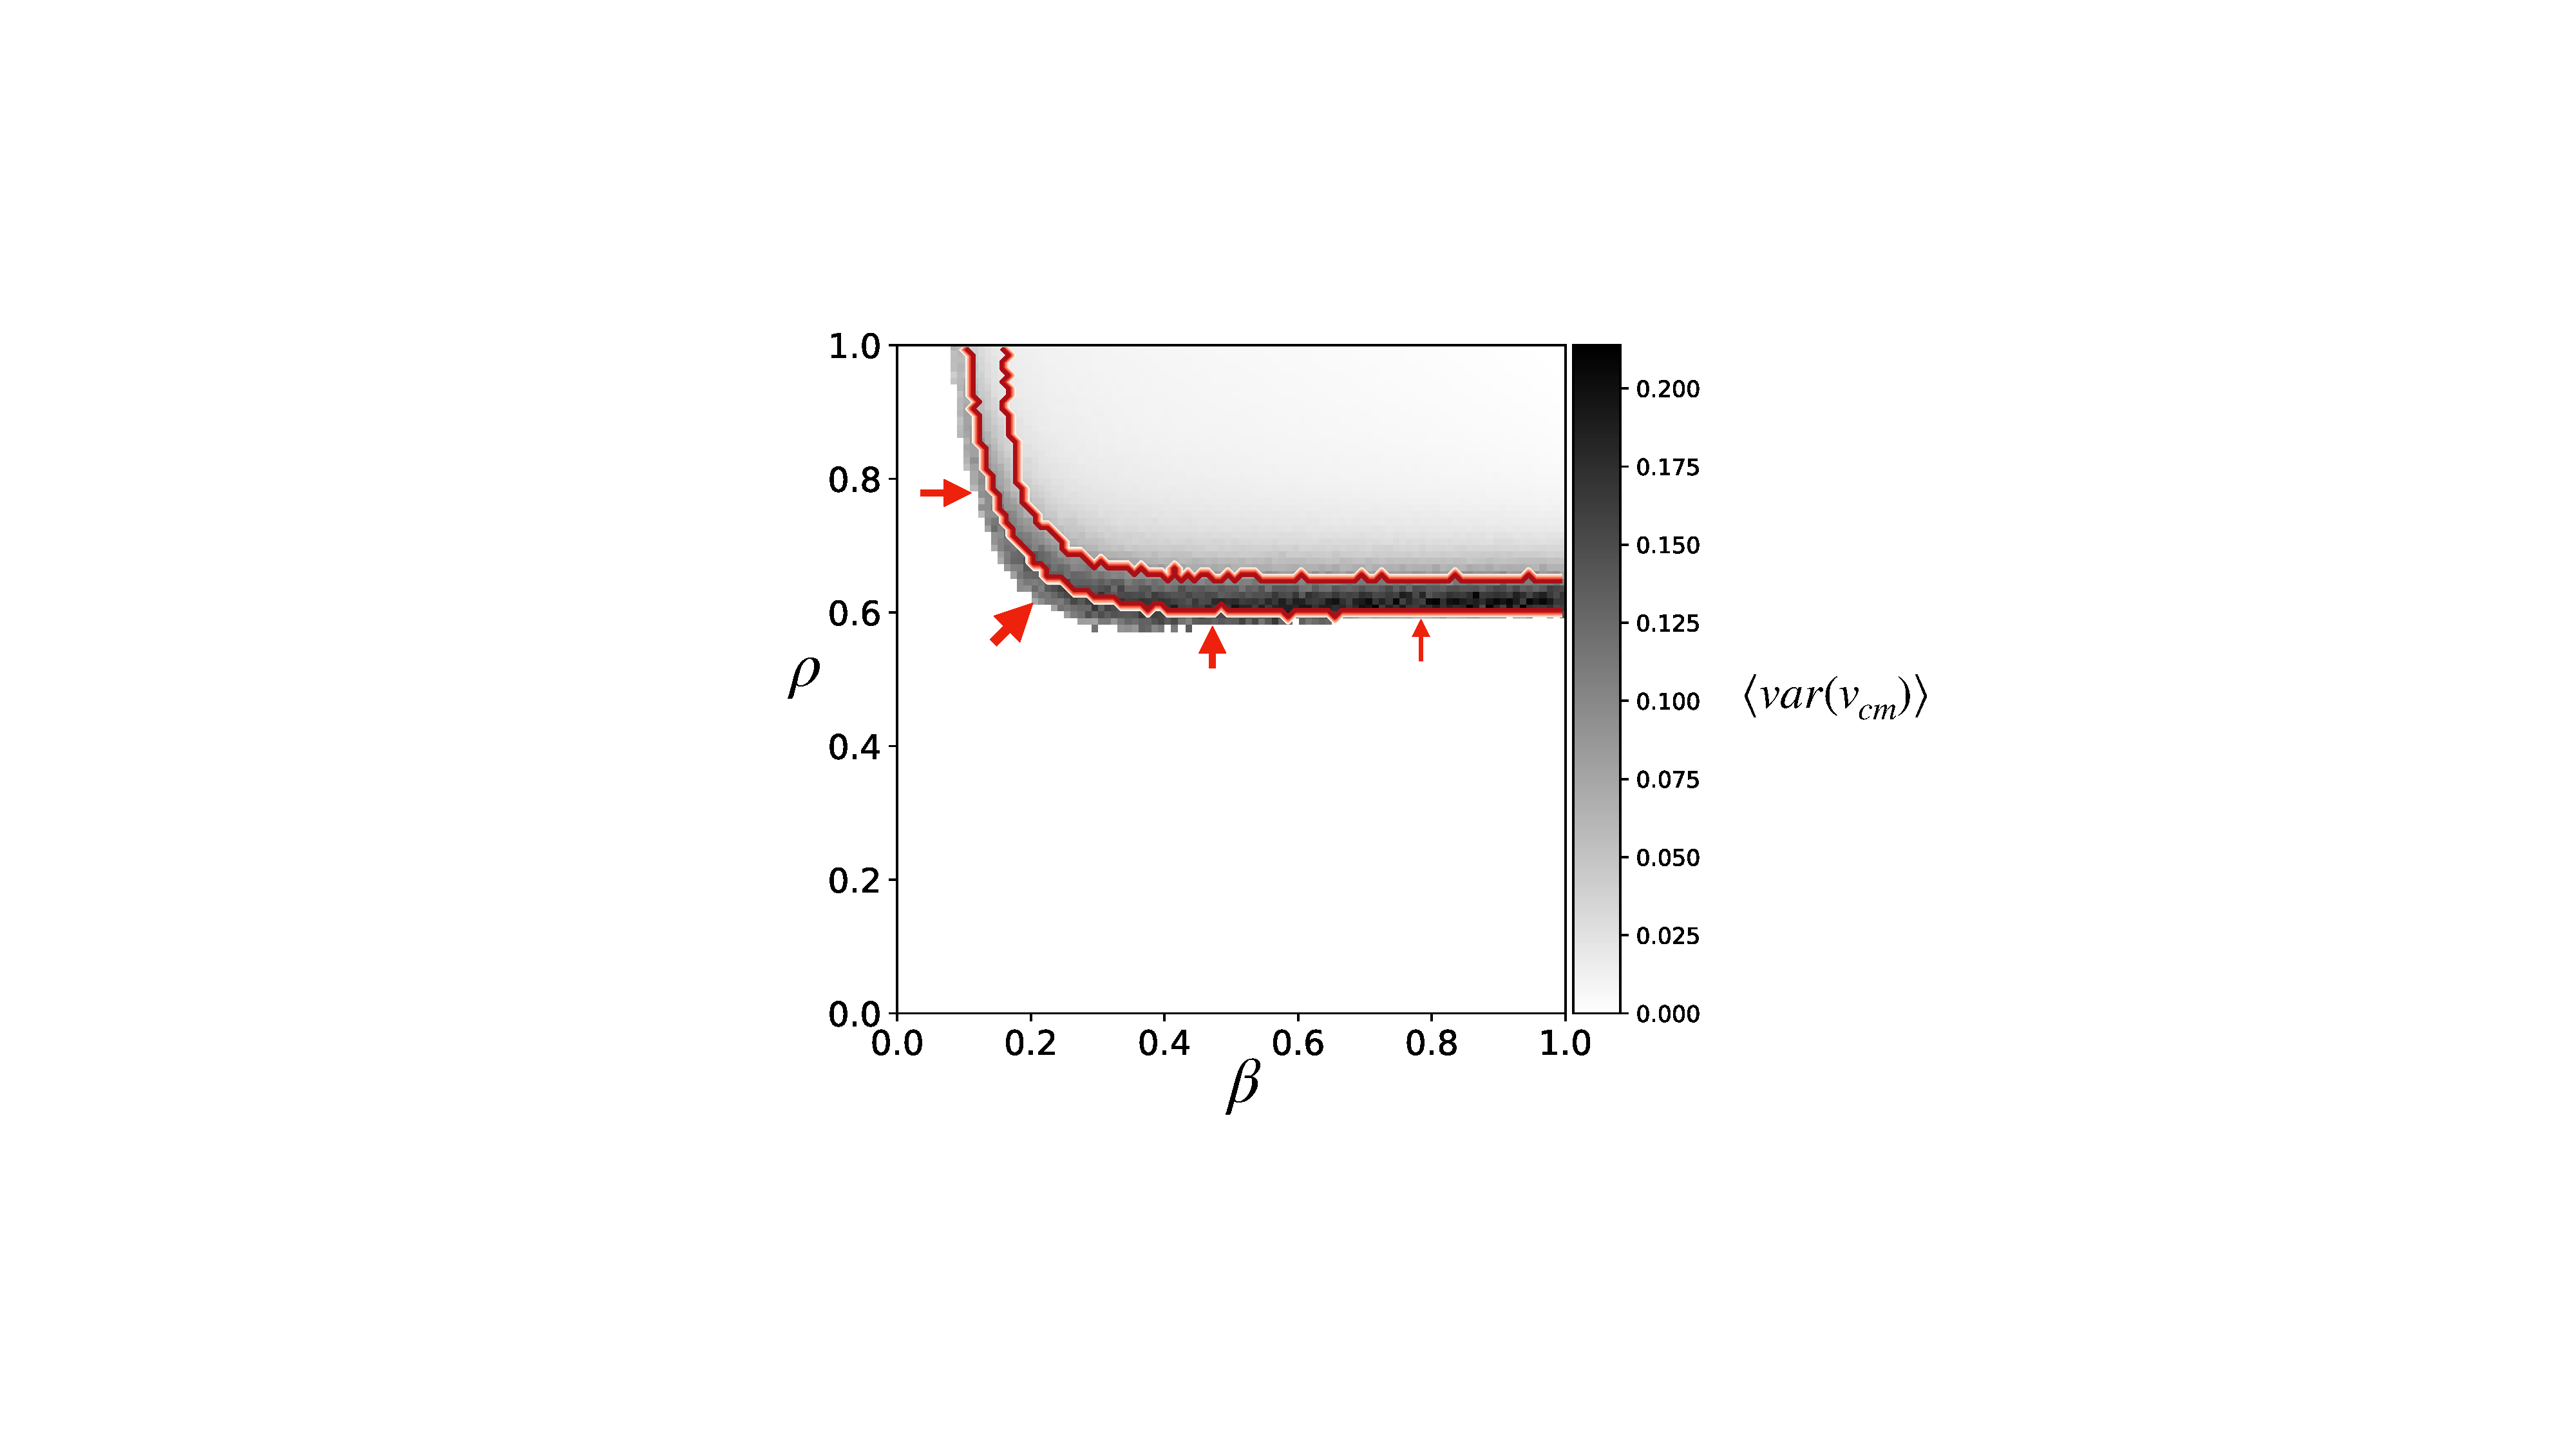
\includegraphics[scale=0.45]{chapter3/figures/figure11.pdf}
    \caption{The ensemble-averaged variance of $v_{cm}(t)$ over a two dimensional parameter sweep of $\rho$ and $\beta$. Red contours show the lower and upper bound of percolation (i.e. between $5\%$ and $95\%$ probability). 
     The epidemic regime is pre-empted by increases in variance more clearly for certain parameter values, %
     indicated by the arrows.}
    \label{fig:ews-results} 
\end{figure}

The following thought experiment can explain the EWS asymmetries in Figure \ref{fig:ews-results}: %
suppose infectivity is high, and density lies just below criticality ($\rho\lesssim\rho_c$), 
so susceptible clusters do not percolate. 
In this case, disease transmission is high on account of $\beta$, 
and all susceptible hosts become quickly infected, 
although an outbreak will come to a halt due to insufficient hosts. Therefore, in this model, 
an aggressive pathogen spreading through low tree densities may propagate rapidly but have a short, 
chaotic signature. Hence the transition is steep,
and the simulation variance is significant, as indicated by the smallest arrow in Figure \ref{fig:ews-results}. 
In this region, detecting an EWS is hard because transitions occur most rapidly.

Now we consider the converse, a less infectious pathogen with an abundance of susceptible hosts, 
located in the top-left region of Figure \ref{fig:ews-results}.
Here, transitions into the $I$ compartment are slower because the pathogen is less infectious, 
although this time, hosts are abundant.
Thus, a pathogen is likely to spread predictably for longer times, 
giving rise to a slightly less abrupt variance signature, 
as indicated by a lighter colour before the transition in the top left quadrant of Figure \ref{fig:ews-primer}.
Although the variance spike is not as significant, 
it preempts the epidemic transition by a more considerable degree\textemdash
indicated by the larger arrows in Figure \ref{fig:ews-results}.
Altogether, Figure \ref{fig:ews-results} suggests that the strength of an EWS depends on the particular combination of epidemic parameters; 
although fundamentally, an EWS is detectable for all parameter combinations
\newpage

\section{A toy landscape-level SLM}

So far, this work has focused on a homogeneous distribution of hosts randomly populating an ideal domain. 
In this section, a toy landscape-level SLM is constructed and simulated on the map of Great Britain.
Modelling the spread of disease over GB entails a large change of scale within the SLM.
Specifically, host units now comprise $\mathrm{1km \times 1km}$ `patches' of land. 
As reviewed in section \ref{ch2:hostdata}, 
collecting high-quality abundance data over large areas is challenging and expensive; 
as such, the SLM is combined with the modelled oak (\textit{Quercus robur}) canopy cover dataset produced by \cite{hill.data}.

\subsection{Realistic boundaries}

Realistic host distributions describe complicated, irregular and heterogeneous domains
known to influence the spread of disease \cite{madden1995plant}.
In contrast, the SLM spreads through a square lattice with regular domain boundaries and homogeneously distributed hosts.
Moreover, the initial conditions (ICs) have been limited to a small number of infected hosts
located at a single epicentre at the centre of a square domain.
However, an epidemic propagating from the centre of a square lattice might look very different
from an epidemic emerging from an arbitrarily located epicentre inside a domain with complicated irregular boundaries.
As a consequence, we examine the interplay of initial and boundary conditions in the SLM\textemdash
compelled further by articles highlighting the importance of domain shape \cite{mikaberidze2016invasiveness},
and critical domain size \cite{abad2020reaction, reimer2017critical}.

As a first step toward modelling with realistic host distribution,
SLM domain edge effects were examined inside the shape of Great Britain.
Figure \ref{fig:uk-spread-primer}(a) shows an outline of Great Britain (GB) filled 
with a random homogeneous distribution of land `patches' at resolution $1\mathrm{km^2}$. 
Here, we change the scale, so host units represent patches of land, 
as opposed to individual trees in chapter \ref{chapter:SLM}.
The green and black pixels represent susceptible and insusceptible patches, 
respectively, as the previous chapter explains.

\begin{figure}
    \centering
    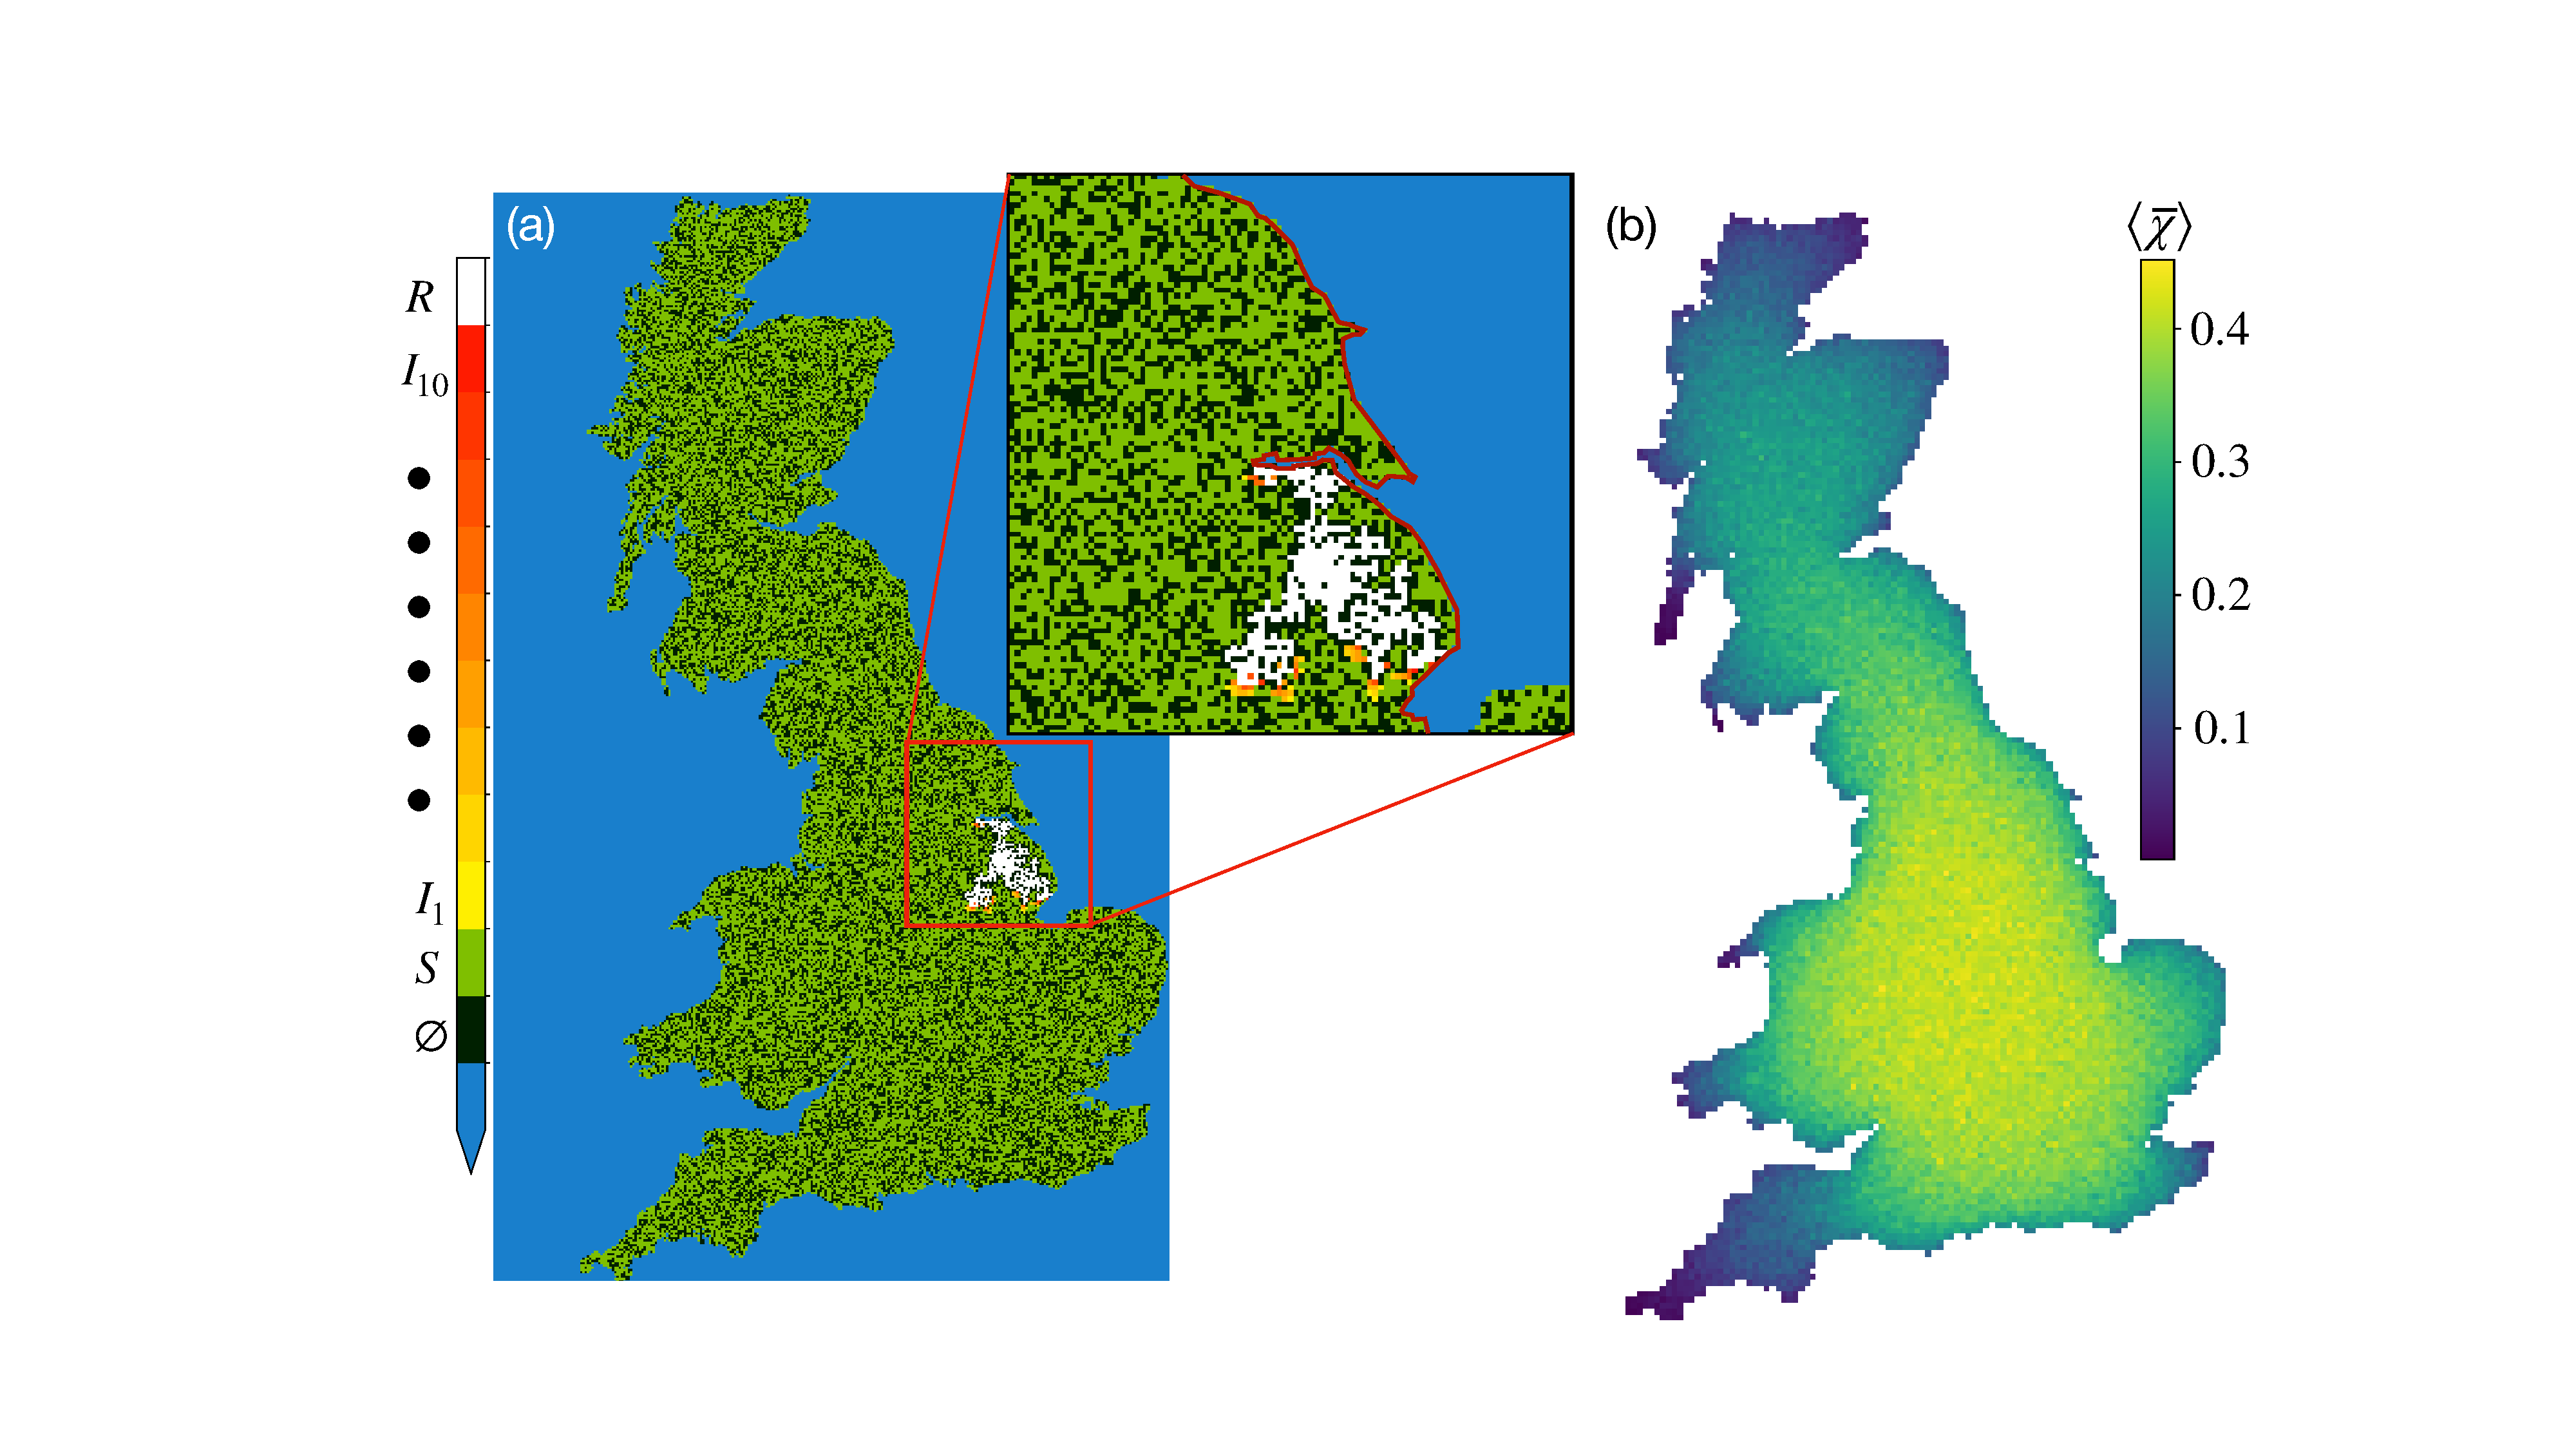
\includegraphics[scale=0.32]{chapter4/figures/figure1-GB-BCs.pdf}
    \caption{(a) The SLM spreading on a map of GB. The domain geometry and epicenter %
    location are non-trivial aspects likely to influence the spread of disease. The zoomed inset %
    shows an example of the Humber estuary preceding an infectious wave-front. 
    (b) Ensemble-averaged mortality-ratios are shown by colour for each spatial location with 
        parameters $\rho=0.65$ and $\beta=0.25$.}
    \label{fig:uk-spread-primer}
\end{figure}

In Figure \ref{fig:uk-spread-primer}(a), we see that coastline edge effects
might reduce the probability of an epidemic.
For example, epidemics emanating from epicentres located just below the 
Humber estuary (shown on the inset) could encounter more impedance when 
compared to more centrally-located positions.
Accordingly, SLM edge effects and domain BCs were examined by assessing the 
tree mortality from every possible epicentre, as shown in Figure \ref{fig:uk-spread-primer}(b).

Figure \ref{fig:uk-spread-primer}(b) reveals the ensemble-averaged mortality 
ratio, denoted by $\chi$.
The toy landscape-level SLM assumed parameter values just above threshold in a $2D$ square lattice. 
Each simulation began from a single patch epicentre, located at position $(i, j)$).
Here, the mortality ratio captures the total epidemic impact, defined by: 
\begin{equation}
\label{eq:epi_impact}
    \chi=\frac{R_f}{S_0}
\end{equation}
where $R_f$ is the final number of patches in the removed state at $T_f$ and $S_0$ is the number of susceptible %
patches at time $T=0$.
Given the system stochasticity, it is necessary to repeat simulations for each epicentre %
and calculate $\overline{\chi}$. Iterating over the whole of the GB in this way permits visualisation
of the spatial-susceptibility of the pathogen $\beta$, depicted by colour in Figure \ref{fig:uk-spread-primer}(b).

Figure \ref{fig:uk-spread-primer}(b) shows the result of the ensemble averaging $\chi$ for each
patch of land\footnote{Ensemble averaging each patch of land was computationally intensive, 
to account for this, the domain resolution was coarse-grained to $\mathrm{5km \times 5km}$ sized-patches.
Simulations were conducted on the Leeds high-performance computing facility, the ARC-HPC system using a task %
array, the ensemble took approximately two hours on $25$ cores.).} 
As expected, the domain BCs and map geometry change the resulting epidemic scale, 
mainly Scotland north of the Anglo-Scottish border and the south Eastern leg of GB towards Exeter and Plymouth;
meanwhile, centralised regions show a roughly constant susceptibility. 
Interestingly, higher epidemic parameters increased the mean mortality ratio and reduced spatial variations
in the mortality ratio, whilst lowering epidemic parameters had the opposite effect.
Although Figure \ref{fig:uk-spread-primer}(b) paints an ideal epidemic scenario involving one infected patch at $t=0$,
we can assume an emerging epidemic within the SLM model depends strongly on the interplay of epicentre location and domain boundary.
 
 \newpage

\subsection{Realistic abundance data}

In Figure \ref{fig:uk-oak-l.hill}(a), the distribution of oak is given by \cite{hill.data} is
plotted over a map of Great Britain, alongside with its corresponding 
probability density function (PDF) in  Figure \ref{fig:uk-oak-l.hill}(b).
Each pixel in Figure \ref{fig:uk-oak-l.hill}(a) depicts the predicted hectares
of oak canopy cover per kilometre squared of land, $\mathrm{ha/km^{2}}$, represented by colour. 
Therefore, each measure of abundance correlates to host density\textemdash
justified by the fact that $100\mathrm{ha} = 1 \mathrm{km^2}$\textemdash expressed as $\rho$.
The spatial map displays visual irregularities and population heterogeneity.

The PDF, $f(\rho)$, displayed in Figure \ref{fig:uk-oak-l.hill}(b) 
reveals that most land patches occupy lower canopy cover values.
Although, a small number ($\sim 5\%$) of high abundance values in the range
$10<\rho<35\ \mathrm{ha/km^2}$ that skewed the distribution were reduced to $10\mathrm{ha/km^2}$, 
thus capping the highest value to $10\%$ of oak canopy cover. 
The PDF describes a continuous distribution in opposition to the binary-valued distribution of hosts 
within the SLM. To navigate this problem, we introduce a threshold function:  
\begin{equation}
  \phi(\rho) =
  \begin{cases}
    1 & \rho_{i,j}\geq\rho \\
    0 & \rho_{i,j}<\rho
  \end{cases}
\end{equation}
where the canopy cover $\rho\in[0, 10]\ \mathrm{ha/km^{2}}$ acts as a threshold value, 
above which all patches become susceptible and assumes the numerical value of unity, i.e. $\rho < \rho_{i,j} = 1$.
Conversely, insusceptible states are described when $\rho \geq \rho_{i,j}= 0$.
The inset of Figure \ref{fig:uk-oak-l.hill}(b) visually depicts the abundance threshold function; 
the vertical black line is an arbitrary threshold $\rho$, and all canopy cover values less and greater than
$\rho$ describe insusceptible and susceptible, respectively.
Susceptible patches have enough hosts to support disease survival, growth, and spread in this interpretation. %
Patches of land below the abundance threshold are presumed insusceptible on account of insufficient hosts.

\newpage

\begin{figure}
    \centering
    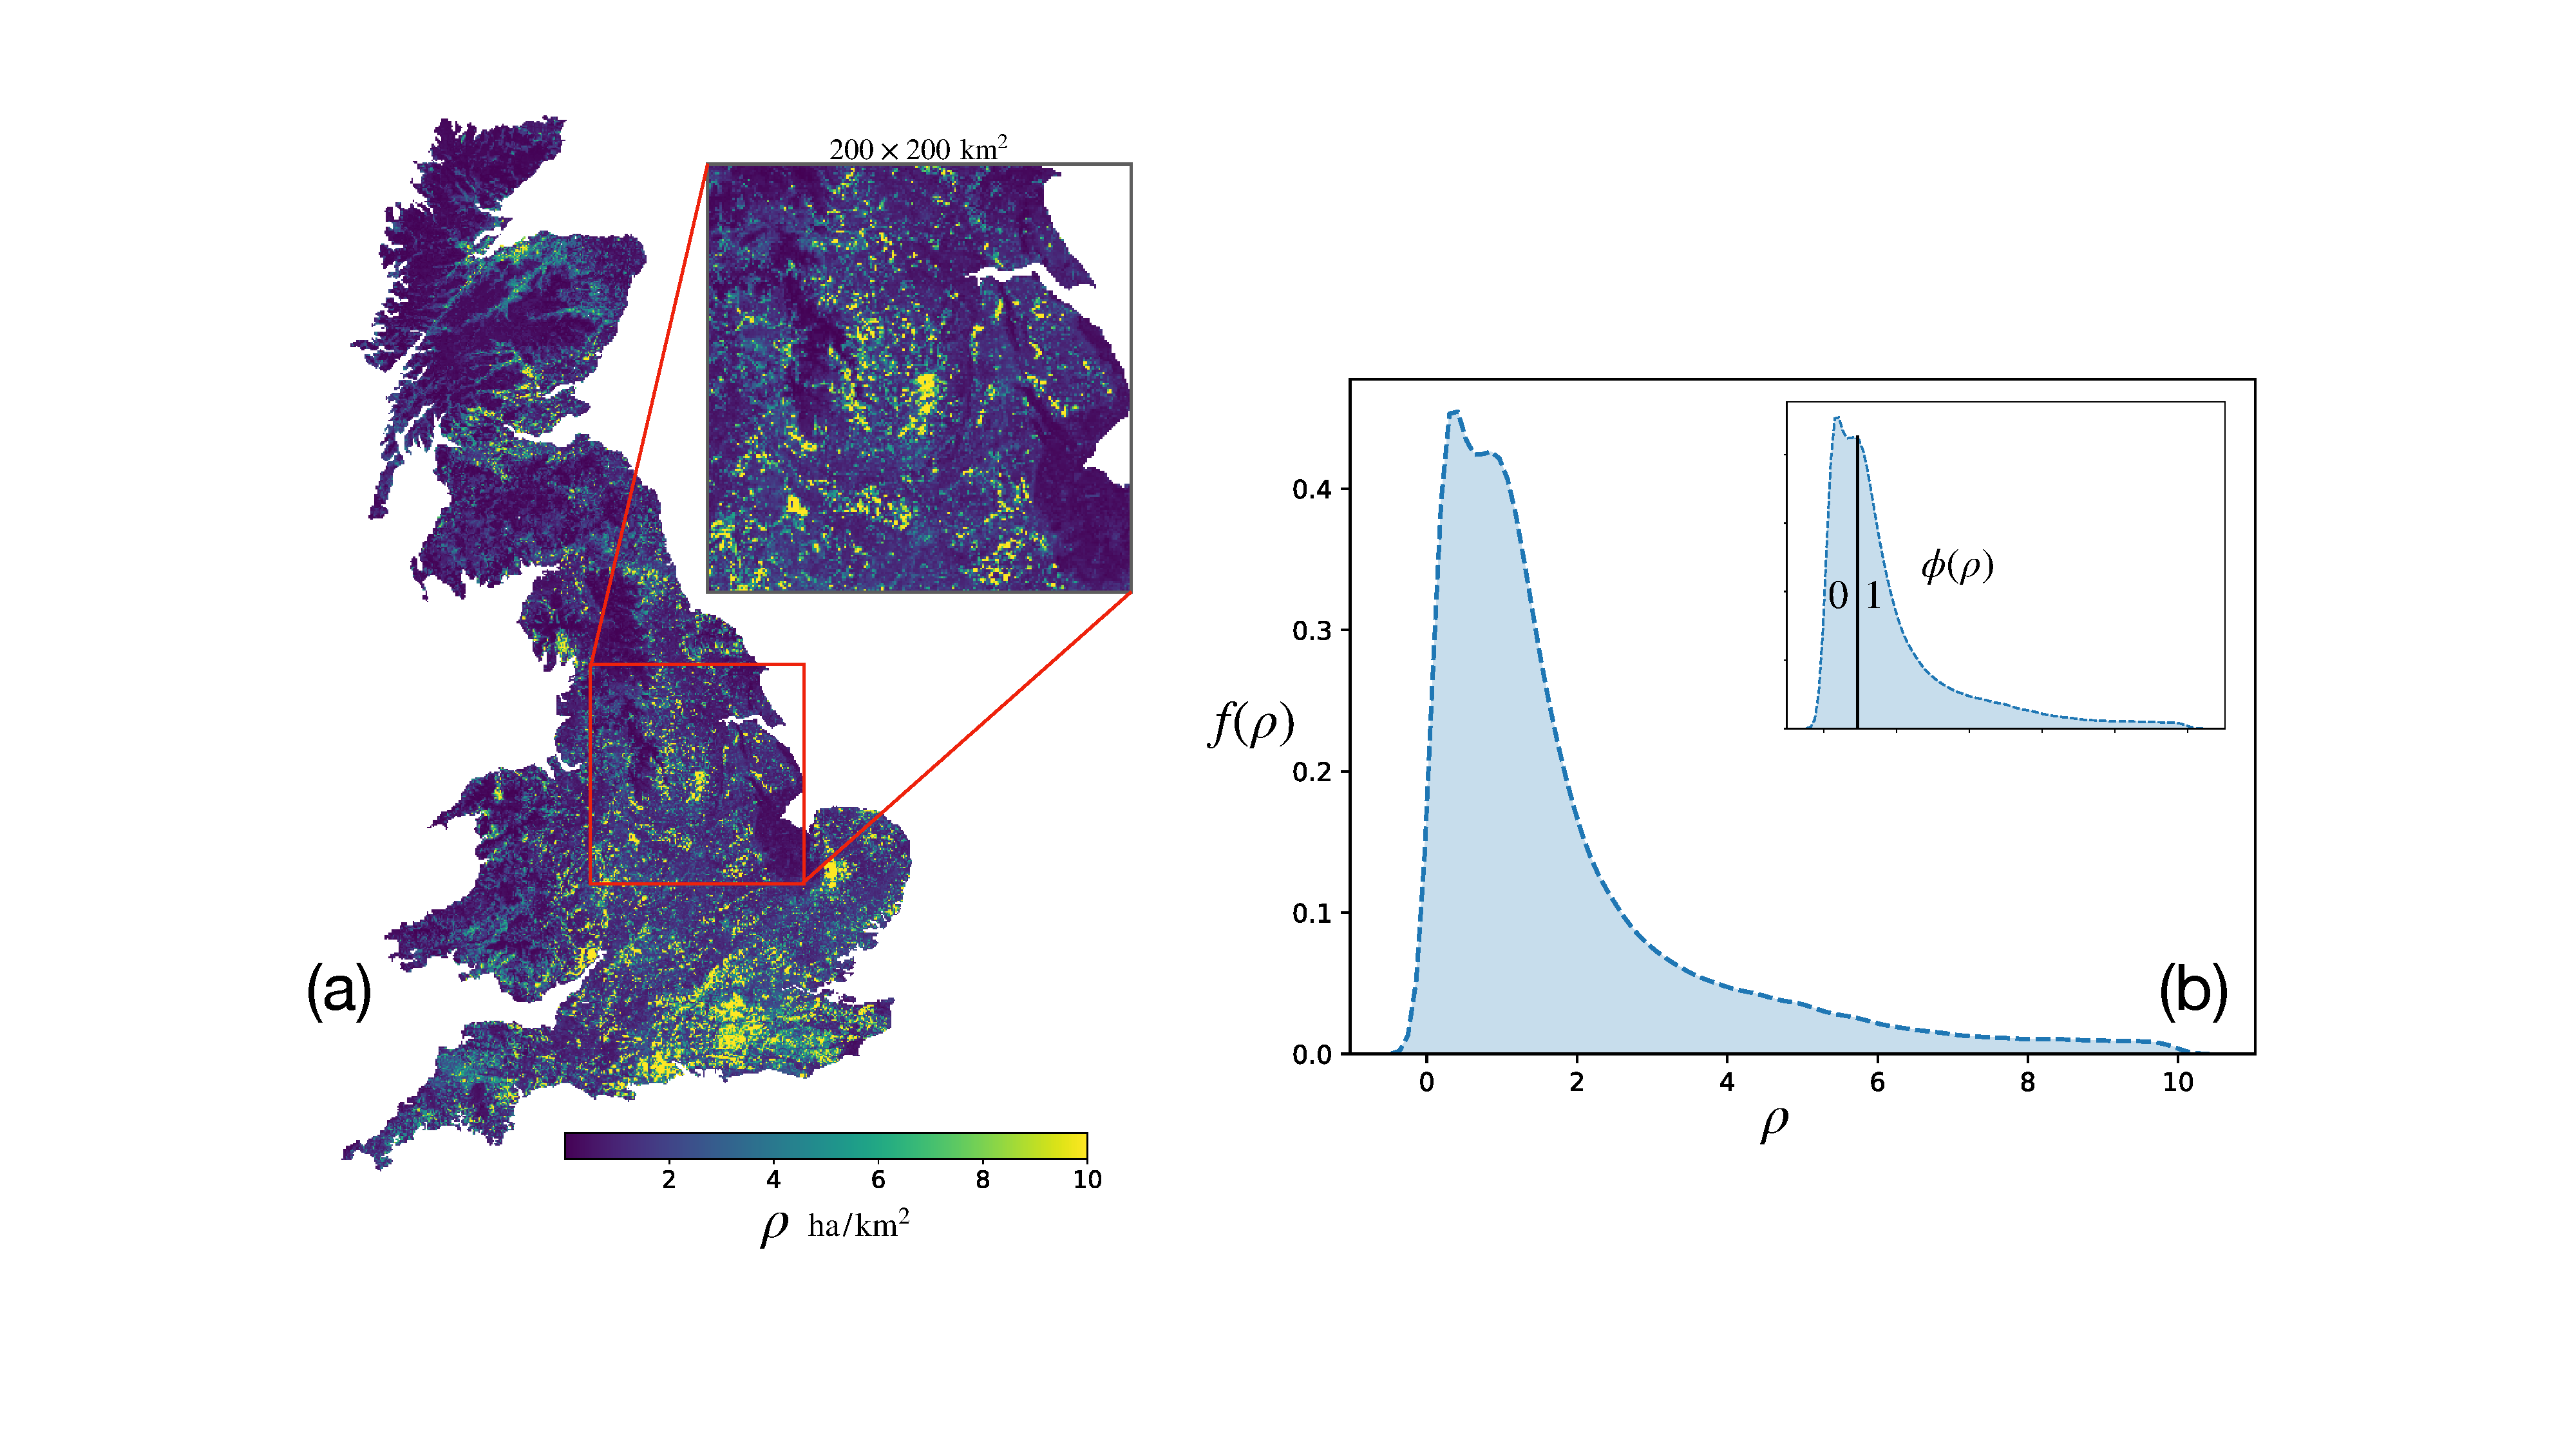
\includegraphics[scale=0.32]{chapter4/figures/figure3.pdf}
    \caption{
    (a) The modelled abundance distribution of common oak (\textit{Quercus robur}), inferred by \cite{hill.data}; each pixel holds a predicted value of abundance having units hectares of canopy cover per kilometer squared of land. 
    (b) The probability density function of abundance $f(\rho) \mathrm{ha/km^2}$. 
    The zoomed inset illustrates the process of generating threshold function $\phi$.}
    \label{fig:uk-oak-l.hill}
\end{figure}

Earlier in chapter \ref{chapter:SLM}, hosts distributions were easily characterised by $\rho \in [0, 1]$, 
describing a uniform density throughout a square lattice.
Now, however, host heterogeneity prevents a simple description of density.
Nevertheless, by considering the percentage of susceptible patches,
one can define effective landscape density $\rho^*$:
\begin{equation}
    \label{eq:rho_eff}
  \rho^{*} = \frac{\sum^{i, j} ( \rho_{i,j} \geq \rho )}{|\mathcal{L}_{GB}|}
\end{equation}
where $\mathcal{L}_{GB}$ represents host distribution over Great Britain. 
The terms $\sum^{i, j} (\rho_{i,j} \geq \rho)$ and $|\mathcal{L}_{GB}|$ represent 
the total number of susceptible patches and total landmass respectively. 
Given an increase in the threshold $\rho$, the effective density $\rho^*$ decreases; 
likewise, a decrease in $\rho$ increases $\rho^*$ as more patches become susceptible. 
Thus, $\rho^{*}$ presents a convenient, although crude, agent
to adjust the host distribution to higher or lower densities.

\subsection{Epidemics through heterogeneous landscapes}

Applying the effective density ($\rho^{*}$) of Equation \ref{eq:rho_eff},
we can initialise a set of binary-valued SLM heterogeneous domains. 
Figure \ref{fig:ch4_uk_spread} shows three variations of effective density
$\rho^{*} \in [0.40, 0.50, 0.60]$, alongside the corresponding thresholds of
abundance canopy cover shown below. In Figure \ref{fig:ch4_uk_spread}, the SLM
is simulated with infectiviy $\beta=0.25$, until pathogen extinction, 
shown through through four time-steps. Between panels (a) (e) and (i), 
the differences in the domain density are visible,
as larger values of abundance thresholds produce lower density maps.
For the three simulations shown in Figure \ref{fig:ch4_uk_spread}, 
epicentres were placed in the south, where the canopy cover is most dense. 

Previously, density was uniform in all directions, 
but now heterogeneity unevenly distributes susceptible hosts. 
Notwithstanding, we may still expect an epidemic to emerge if density 
and infectivity parameters satisfy a critical threshold, as explored in chapter \ref{chapter:SLM}.
For all $\rho^*$ values shown in Figure \ref{fig:oak-spatial-ensemble}, 
initial outbreaks ($0<t<250$) spread above the threshold.
Although at $\rho^*=0.40$, we notice a significant drop in disease progression 
beyond $t=250$ in (c-d), approximately extending from Oxford to Buckinghamshire due to a low density;
in contrast, $\rho^*=0.50$ and $\rho^*=0.60$ spread above the threshold for all panels.

In Figure \ref{fig:ch4_uk_spread} we can observe a spatial dependence in the SLM threshold,
where above-threshold regions (e.g. the in south) depend on the host density $\rho^*$ parameter.
In particular, Figure \ref{fig:ch4_uk_spread} demonstrates that increasing $\rho^*$ can lead to channels opening between different above-threshold regions, thus permitting disease to invade new regions, c.f. Figure \ref{fig:ch4_uk_spread}(d), (h), and (l) where higher density simulations spread progressively further northwards.
Undesirably, percolation is hard to define in the domain configuration shown in 
Figure \ref{fig:oak-spatial-ensemble} because the extent between borders is now non-uniform
and dependant on epicentre location.
Furthermore, simulation time series are subject to additional noise on account of heterogeneity, 
making velocity-based metrics such as Equation \ref{eq:vel_eff_r} hard to use. 
Subsequently, the examination of disease progression will focus on the mortality ratio $\chi$, 
as its measurement depends only on the final value of removed trees.

\begin{figure}
    \centering
    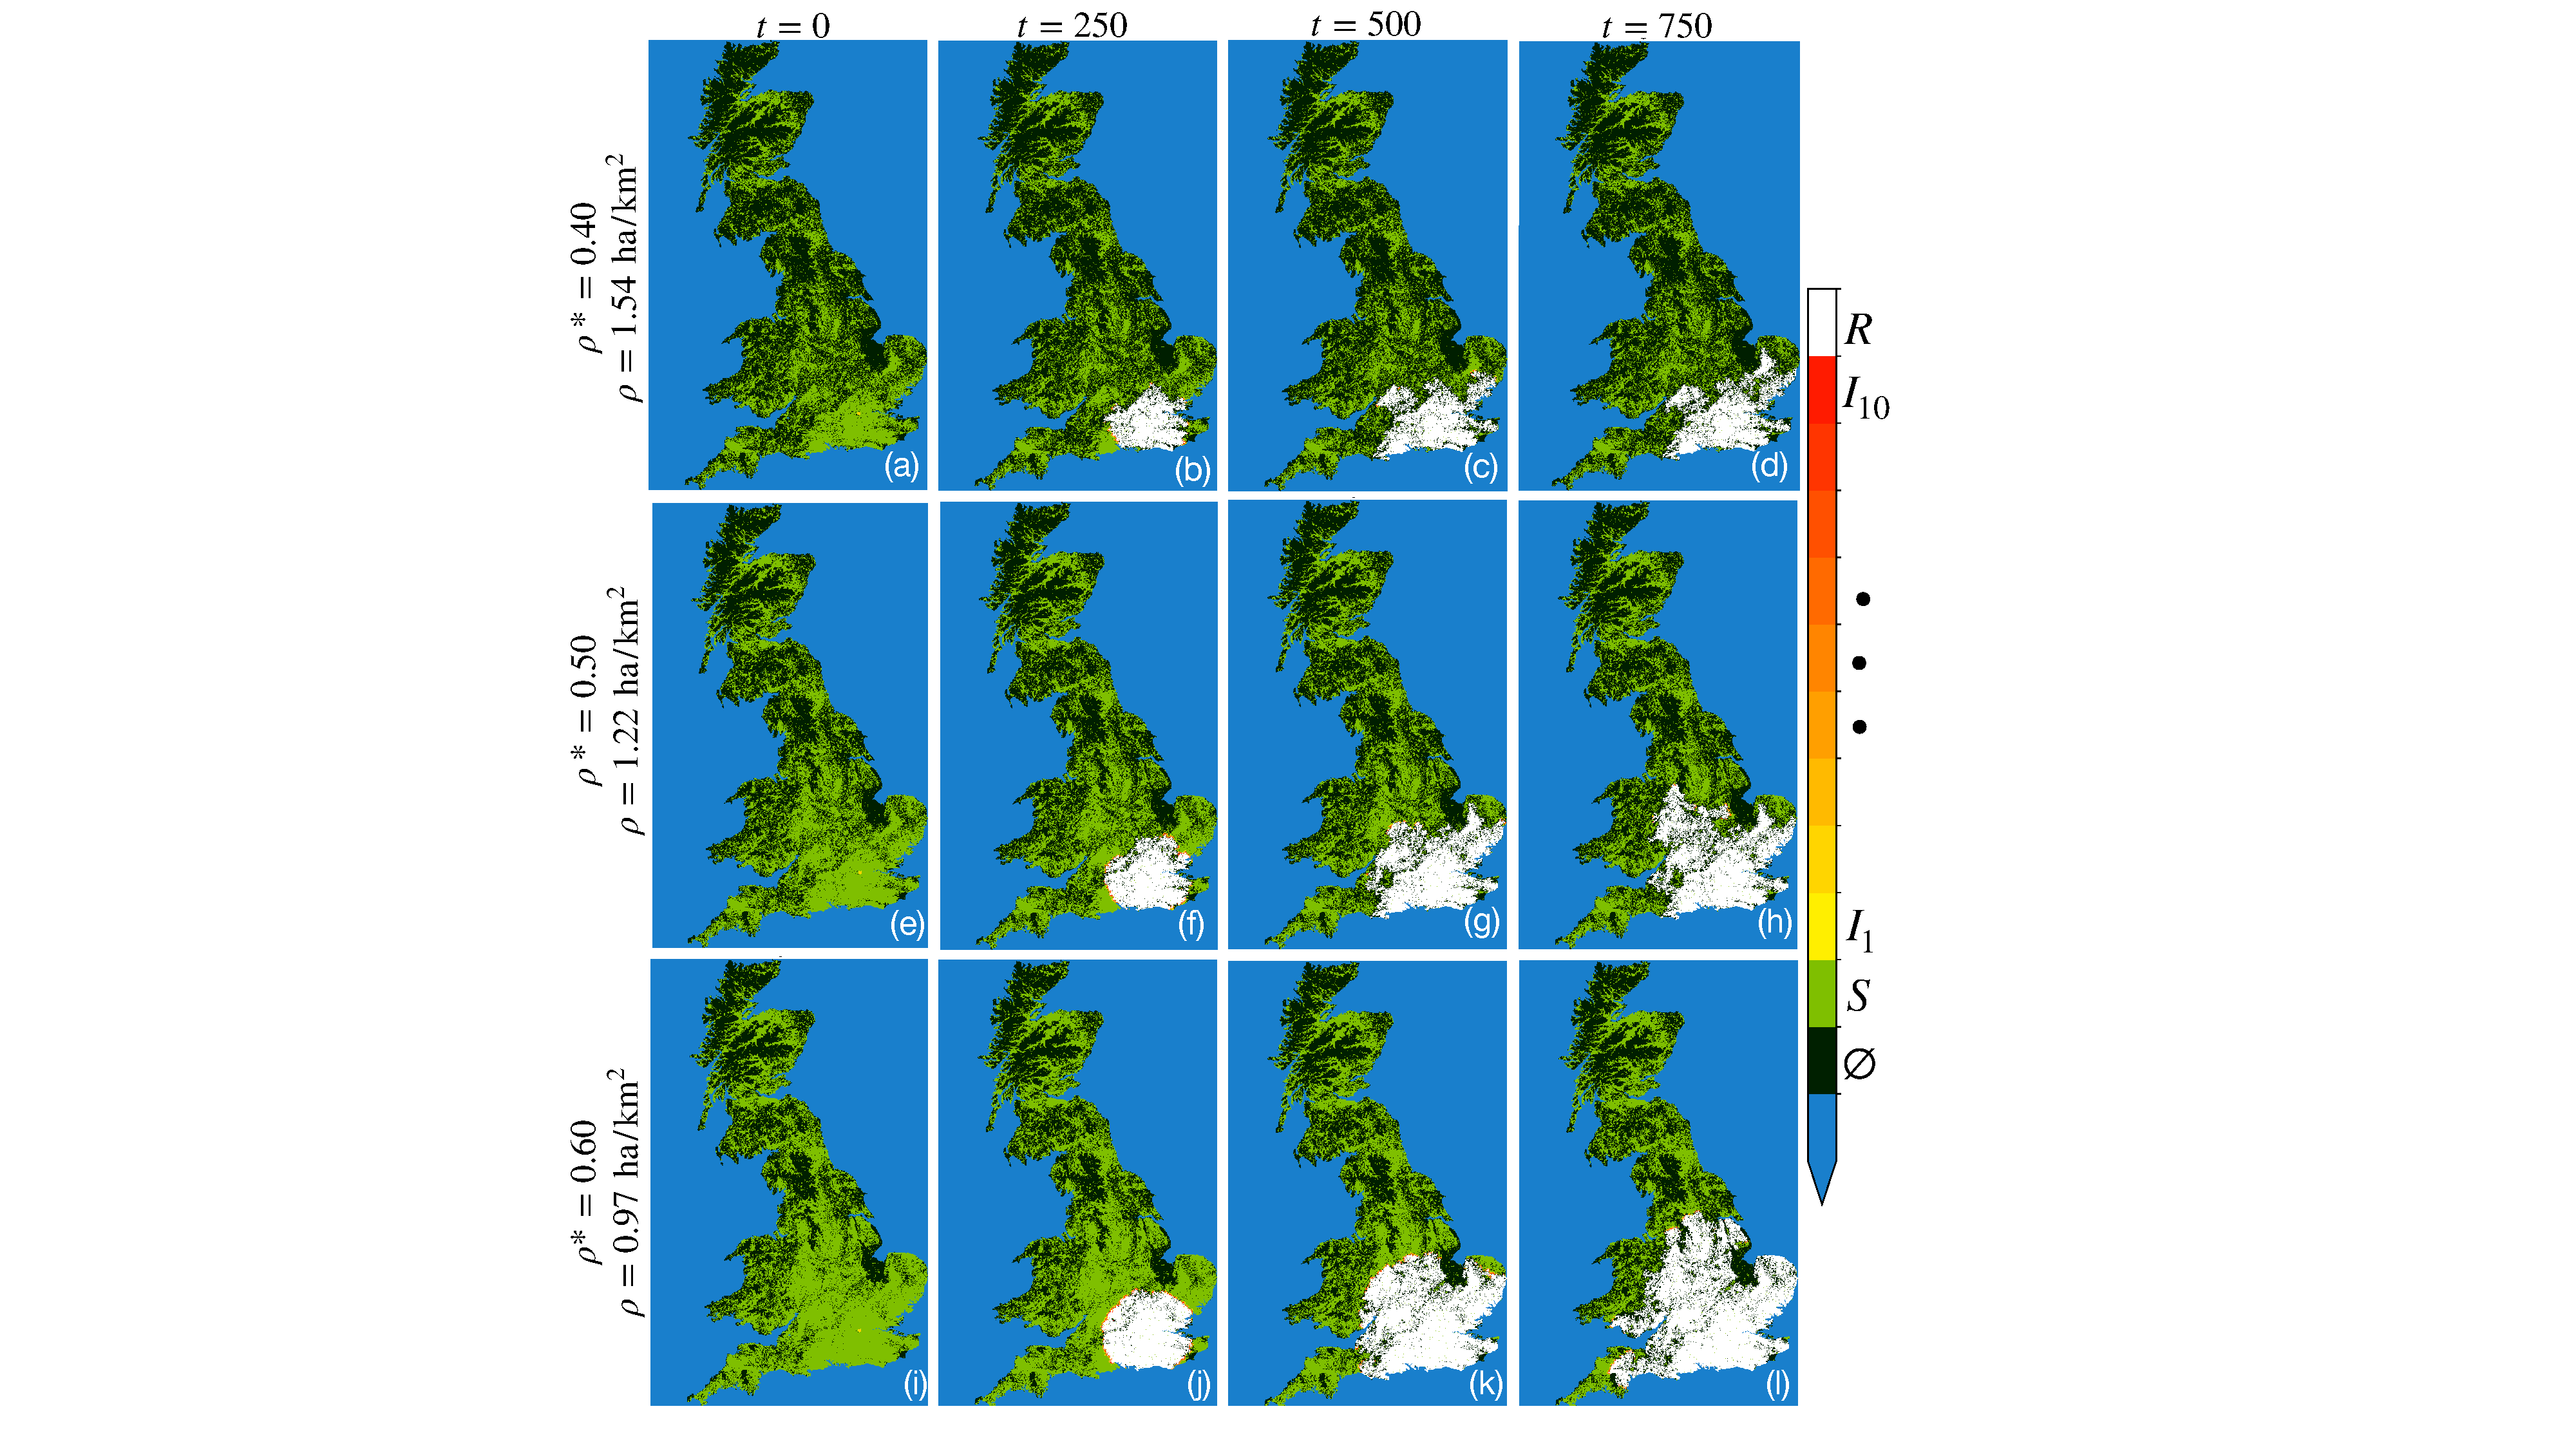
\includegraphics[scale=0.490]{chapter4/figures/figure4.pdf}
    \caption{The simple lattice model running on a binary-valued Oak domain with infectivity $\beta=0.25$ for three variations of effective density $\rho^*$.}
    \label{fig:ch4_uk_spread}
\end{figure}

\subsection{Spatially dependent ensembles}
\label{sec:slm-spatial-ensembles}

The observations of spatially varying thresholds, as suggested by Figure \ref{fig:ch4_uk_spread}, 
motivates an examination of epidemic impact as a function of epicentre location.
As such, we apply the same ensemble averaging method discussed previously (in Figure \ref{fig:uk-spread-primer})
to the oak abundance data set. That is, treating each location $(i,j)$ in GB as a potential
epicentre and ensemble averaging host mortality over many simulations.
Here, the mortality ratio $\big\langle \overline{\chi} \big\rangle \in [0, 1]$ describes the ratio 
of removed host patches to the total number of susceptible patches at $t=0$ and 
expresses the final sized epidemic in the SLM. 

The results of spatial ensemble averaging simulations are shown in Figure \ref{fig:oak-spatial-ensemble},
for three different effective densities and one value of infectivity $\beta=0.25$. 
The values of effective density in Figure \ref{fig:oak-spatial-ensemble} are arbitrary
but crucially exhibit the heterogeneous SLM behaviour. Unsurprisingly, increasing the effective density yields a 
higher mortality ratio (as defined by Equation \ref{eq:epi_impact}), thus increasing the magnitude of successive 
colour bars in Figures \ref{fig:oak-spatial-ensemble}(a-c). Alongside a more severe mortality ratio, a higher $\rho^*$
value permits disease propagation over more extensive regions, witnessed by comparing Figures \ref{fig:oak-spatial-ensemble}(a) and (c).

In Figures \ref{fig:oak-spatial-ensemble}(a-c), yellow regions highlight where the pathogen is most 
likely to spread through susceptible hosts. In this toy model, mortality is approximately independent of epicentre location, 
provided sufficient (Von Neumann) connectivity between patches, supported by uniform yellow contours within susceptible regions.
In panel (a), the spatial locations encircled in dashed red highlight a region of instability that appears to separate two susceptible regions.
In these regions, the epidemic impact could vary significantly, 
consequently prompting the corresponding plots of mortality variance in Figures \ref{fig:oak-spatial-ensemble}(d-f).

\begin{figure}
    \centering
    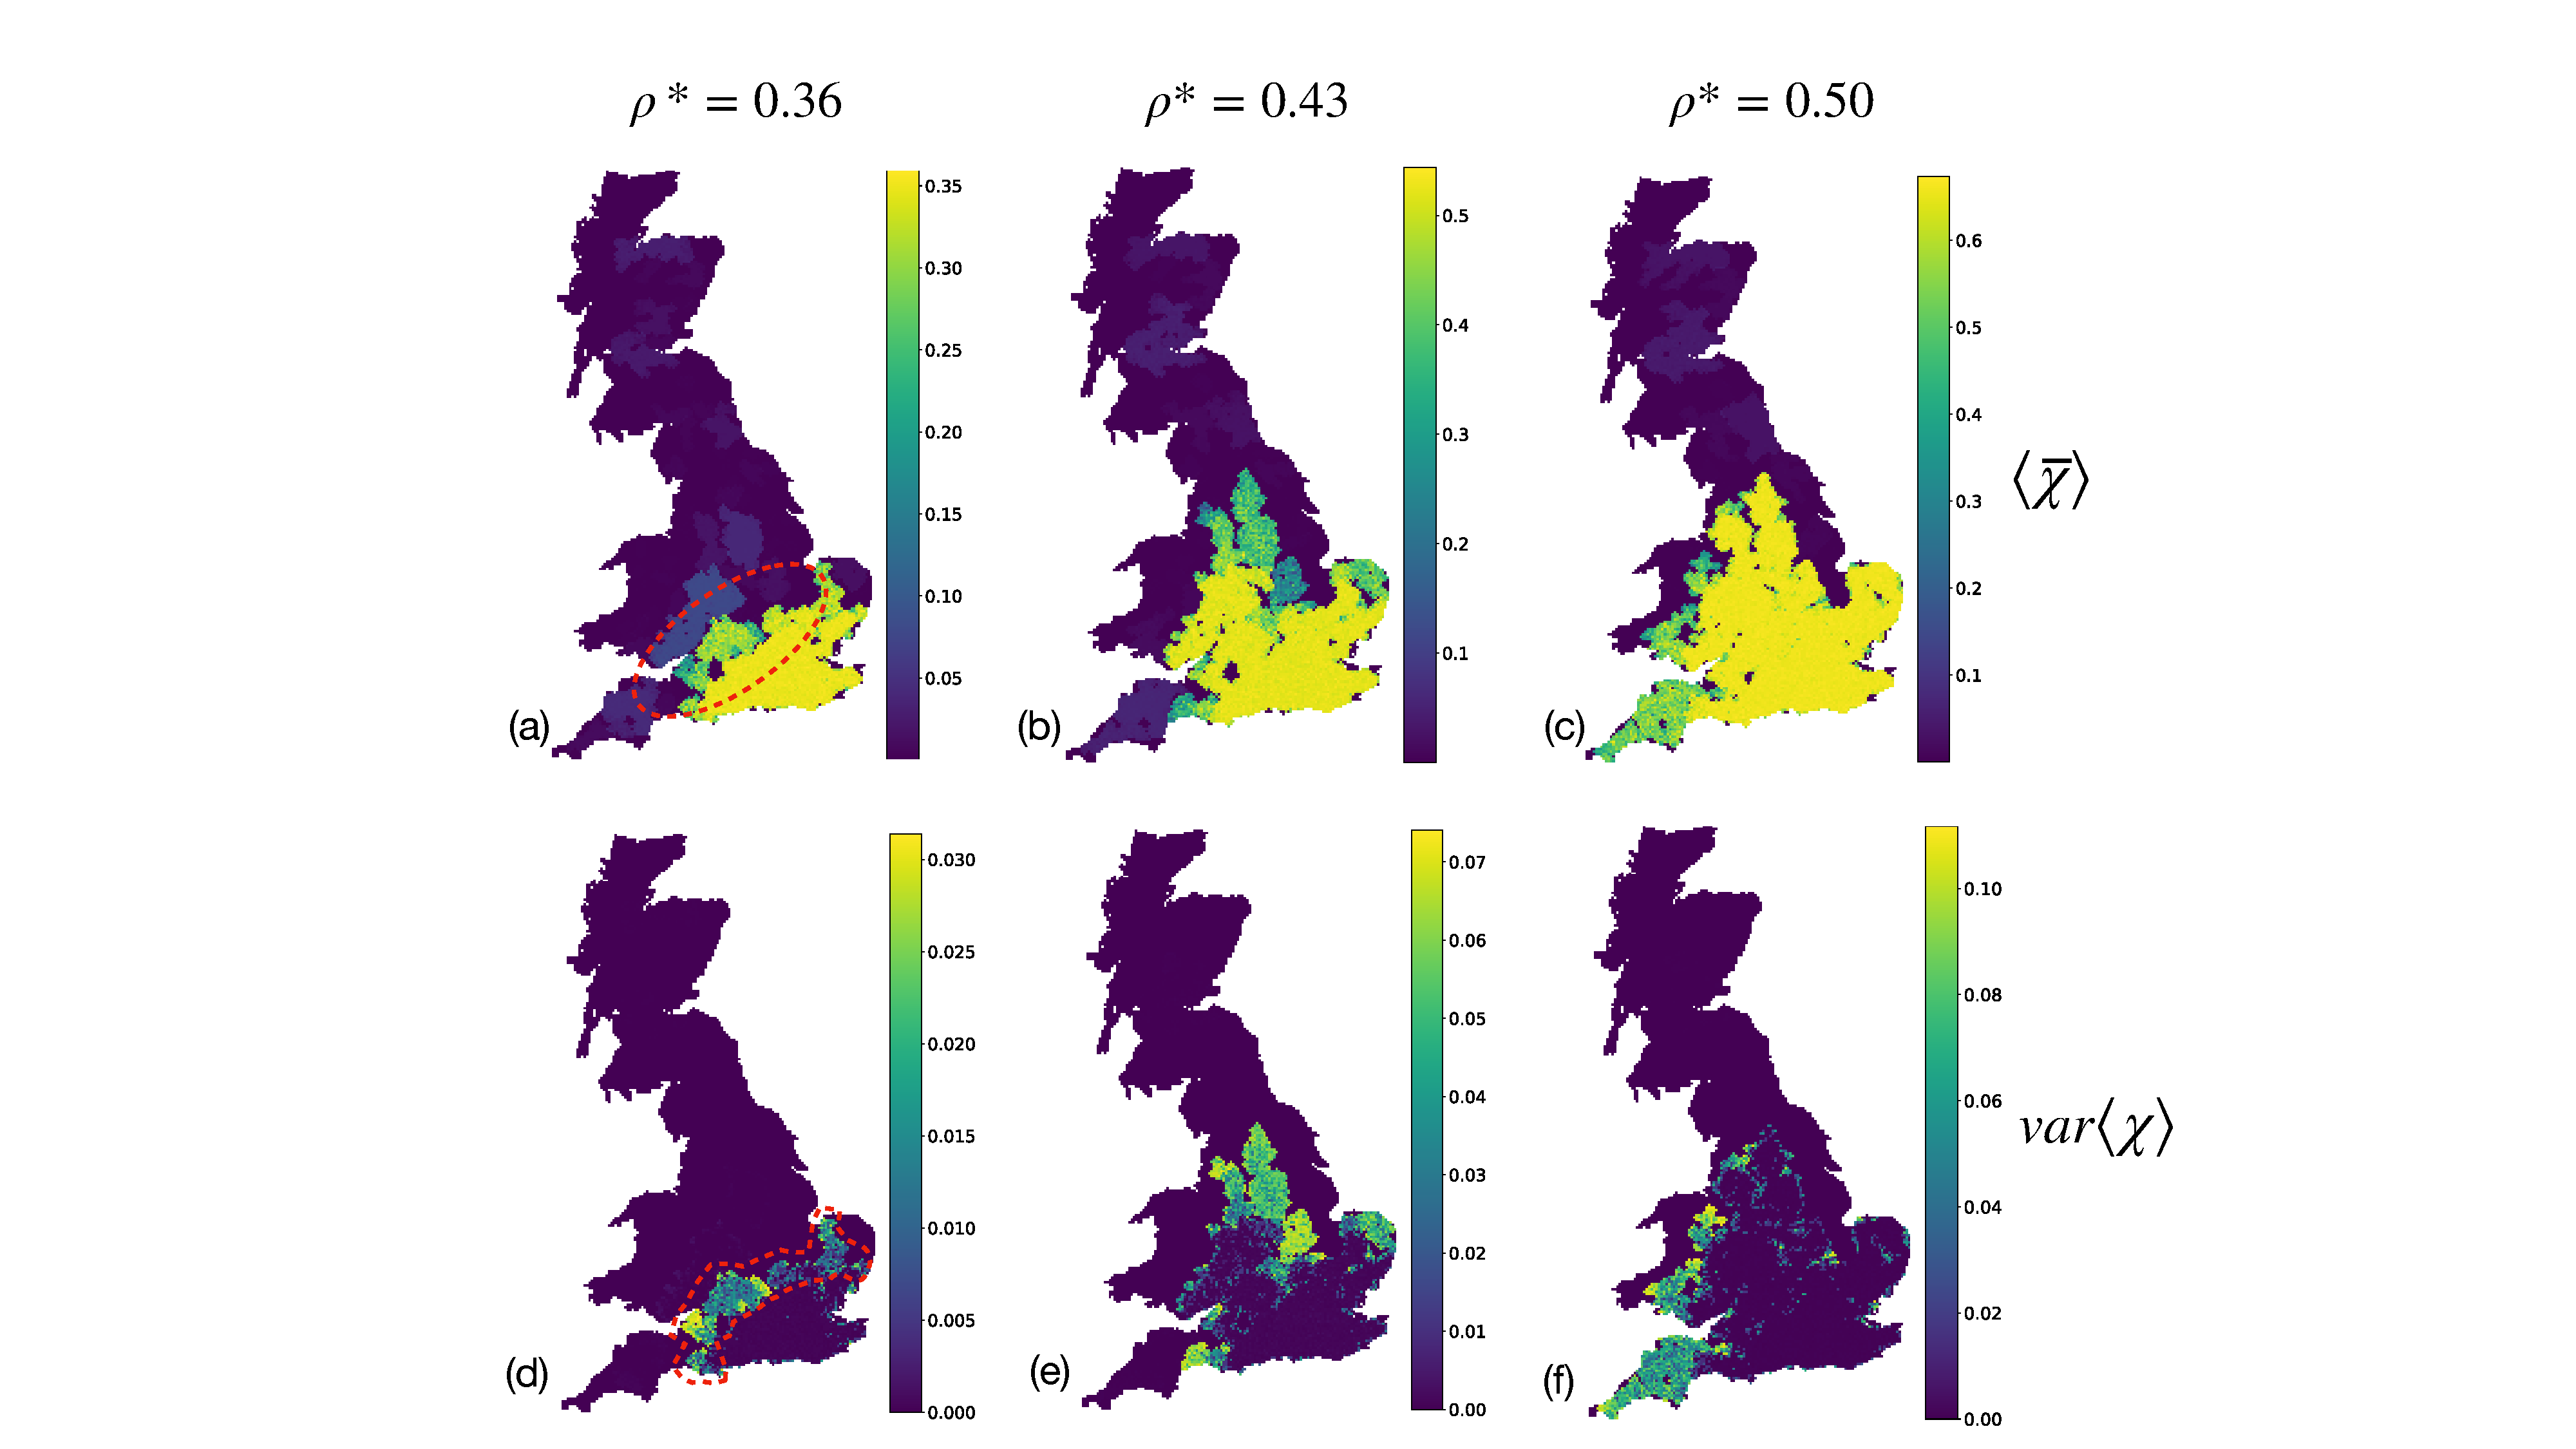
\includegraphics[scale=0.4]{chapter4/figures/figure5.pdf}
    \caption{Spatial phase showing ensemble statistics over the oak data-set for three variations of density threshold $\phi(\rho): \rho \in [0.37, 0.43, 0.50]$ and fixed infectivity $\beta=0.25$. (a-c) The ensemble mean of mortality ratio $\chi$ measured for each pixel epicenter. The dotted red circle in Fig (a) shows two neighbouring susceptible regions. (d-f) Ensemble variance over $\chi$. The dotted shape in (d) highlights an unstable region of high variance and uncertainty separating two susceptible areas of the population in Fig (a).}
    \label{fig:oak-spatial-ensemble}
\end{figure}
Plotting the mortality ensemble variance illustrates where epidemic outcomes can go either direction, 
where the possibility of large-scale epidemic and pathogen extinction exists simultaneously in the parameter regime.
Figure \ref{fig:oak-spatial-ensemble}(d) captures a centrally-located region of uncertainty, highlighted in red; 
in these regions, the toy model may or may not give rise to a large scale epidemic, as opposed to the most southerly, 
high-mortality region beneath the dashed red lines. Panels (e) and (f) show a variance only in the edges of the centrally
located susceptible region. It is alluring to consider the implications of high variance regions in Figures \ref{fig:oak-spatial-ensemble}(d-f)
in the context of epidemic control. Namely, we may suppose that epidemic control through high variance regions could be an effective strategy
in stopping the spread of disease.
Although the mortality ratio ($\chi$) categorises the overall epidemic scale in the SLM, 
it fails to reflect any information about how far an epidemic is likely to propagate.
Recording the maximum distance travelled by the pathogen proved a helpful method to illustrate spatial progression,
maps of `maximum distance' are displayed in appendix \ref{a:landscape-toy-model}. 


\subsection{Heterogeneous parameter sweeps}

Ensemble analysis has so far fixed infectivity to $\beta=0.25$
and instead concentrated on mapping mortality with a varying effective density parameter $\rho^*$.
In this section, we investigate the entire parameter space of $\rho^*$ and $\beta$.
Figure \ref{fig:heterogeneous-phase-space} depicts a full parameter sweep of the toy landscape SLM.
Due to more host units in computer memory, simulating the spread of disease in the toy landscape SLM is more 
computationally challenging when compared to the ideal square SLM in chapter \ref{ch3:two-param-model}.
Even though epidemic progression in the SLM is conditioned on epicentre location (as confirmed by the findings of section \ref{sec:slm-spatial-ensembles}),
analysing a single epicentre is sufficient to capture the essential toy model behaviour.
Ergo, we present an analysis through a single epicentre.

Figure \ref{fig:heterogeneous-phase-space} shows the ensemble-averaged epidemic phase space of the toy landscape SLM
through a epicentre\textemdash indicated by the red point in Figure \ref{fig:heterogeneous-phase-space}(a).
The Parameter sweeps of $\rho^{*}$ and $\beta$ demonstrate multiple discontinuities and sharp increases in $\chi$
for particular combinations of $\rho^{*}$ and $\beta$; this contrast with the parameter sweeps inside a homogeneous square domain.
Moreover, Figure \ref{fig:heterogeneous-phase-space}(b) reveals a large asymmetry between $\rho^*$ and $\beta$ 
as more discontinuous jumps appear most when $\rho^*$ is increased, i.e. moving horizontally 
through Figure \ref{fig:heterogeneous-phase-space}(b). Hence, host heterogeneity gives rise to distinct behaviours for both
$\rho^*$ and $\beta$ axes, as opposed to the (approximately) symmetric ensembles in a homogeneous square domain.  

Figures \ref{fig:heterogeneous-phase-space}(c-d) contrast behavioural differences between 
$\rho^*$ and $\beta$ axes. Specifically, we compare one-dimensional slices through both parameters $\rho^*$ and $\beta$.
Figure \ref{fig:heterogeneous-phase-space}(d) details how variations of $\rho^*$ effect the model behaviour through $\beta$-space. 
Interestingly, Figure \ref{fig:heterogeneous-phase-space}(d) depicts the same infectivity threshold of $\beta\sim0.10$, 
identical to the SLM evolving on a uniform square domain. When $\beta$ increases, fewer discontinuities arise when
compared to $\rho^*$, as evidenced by smoother curves. 

For each value of density in Figure \ref{fig:heterogeneous-phase-space}(d), 
the mortality remains fixed beyond $0.30 \lessapprox \beta$.
We may understand the independence between $\chi$ and infectivity through a numerical example:
the probability of a susceptible patch remaining susceptible when it encounters 
an infected neighbour is given by Equation \ref{eq:pr_s_s} as $Pr(S \rightarrow S) = (1 - 0.30)^{10} = 0.03$. 
Therefore, on average the pathogen transmits successfully to susceptible neighbours with probability $Pr(S\rightarrow I)=0.97$, 
e.g. if a particular epicentre belongs to a susceptible region containing $100$ patches, only three patches remain susceptible. 
In this instance, most patches in the cluster become infected, and further increases in $\beta$ do not affect the 
mortality\footnote{
Increasing the infectivity to $\beta=0.40$ yields a $Pr(S \rightarrow S) = 0.006$, 
leading to negligible changes in the final epidemic size\textemdash however, the rate of progression is still faster.
}. 
When $0.30 \sim \beta$, only increases to the domain density have the potential to raise the final epidemic size, 
indicated by the increases in the height of the curves in Figure \ref{fig:heterogeneous-phase-space}(d). 

\begin{figure}
    \centering
    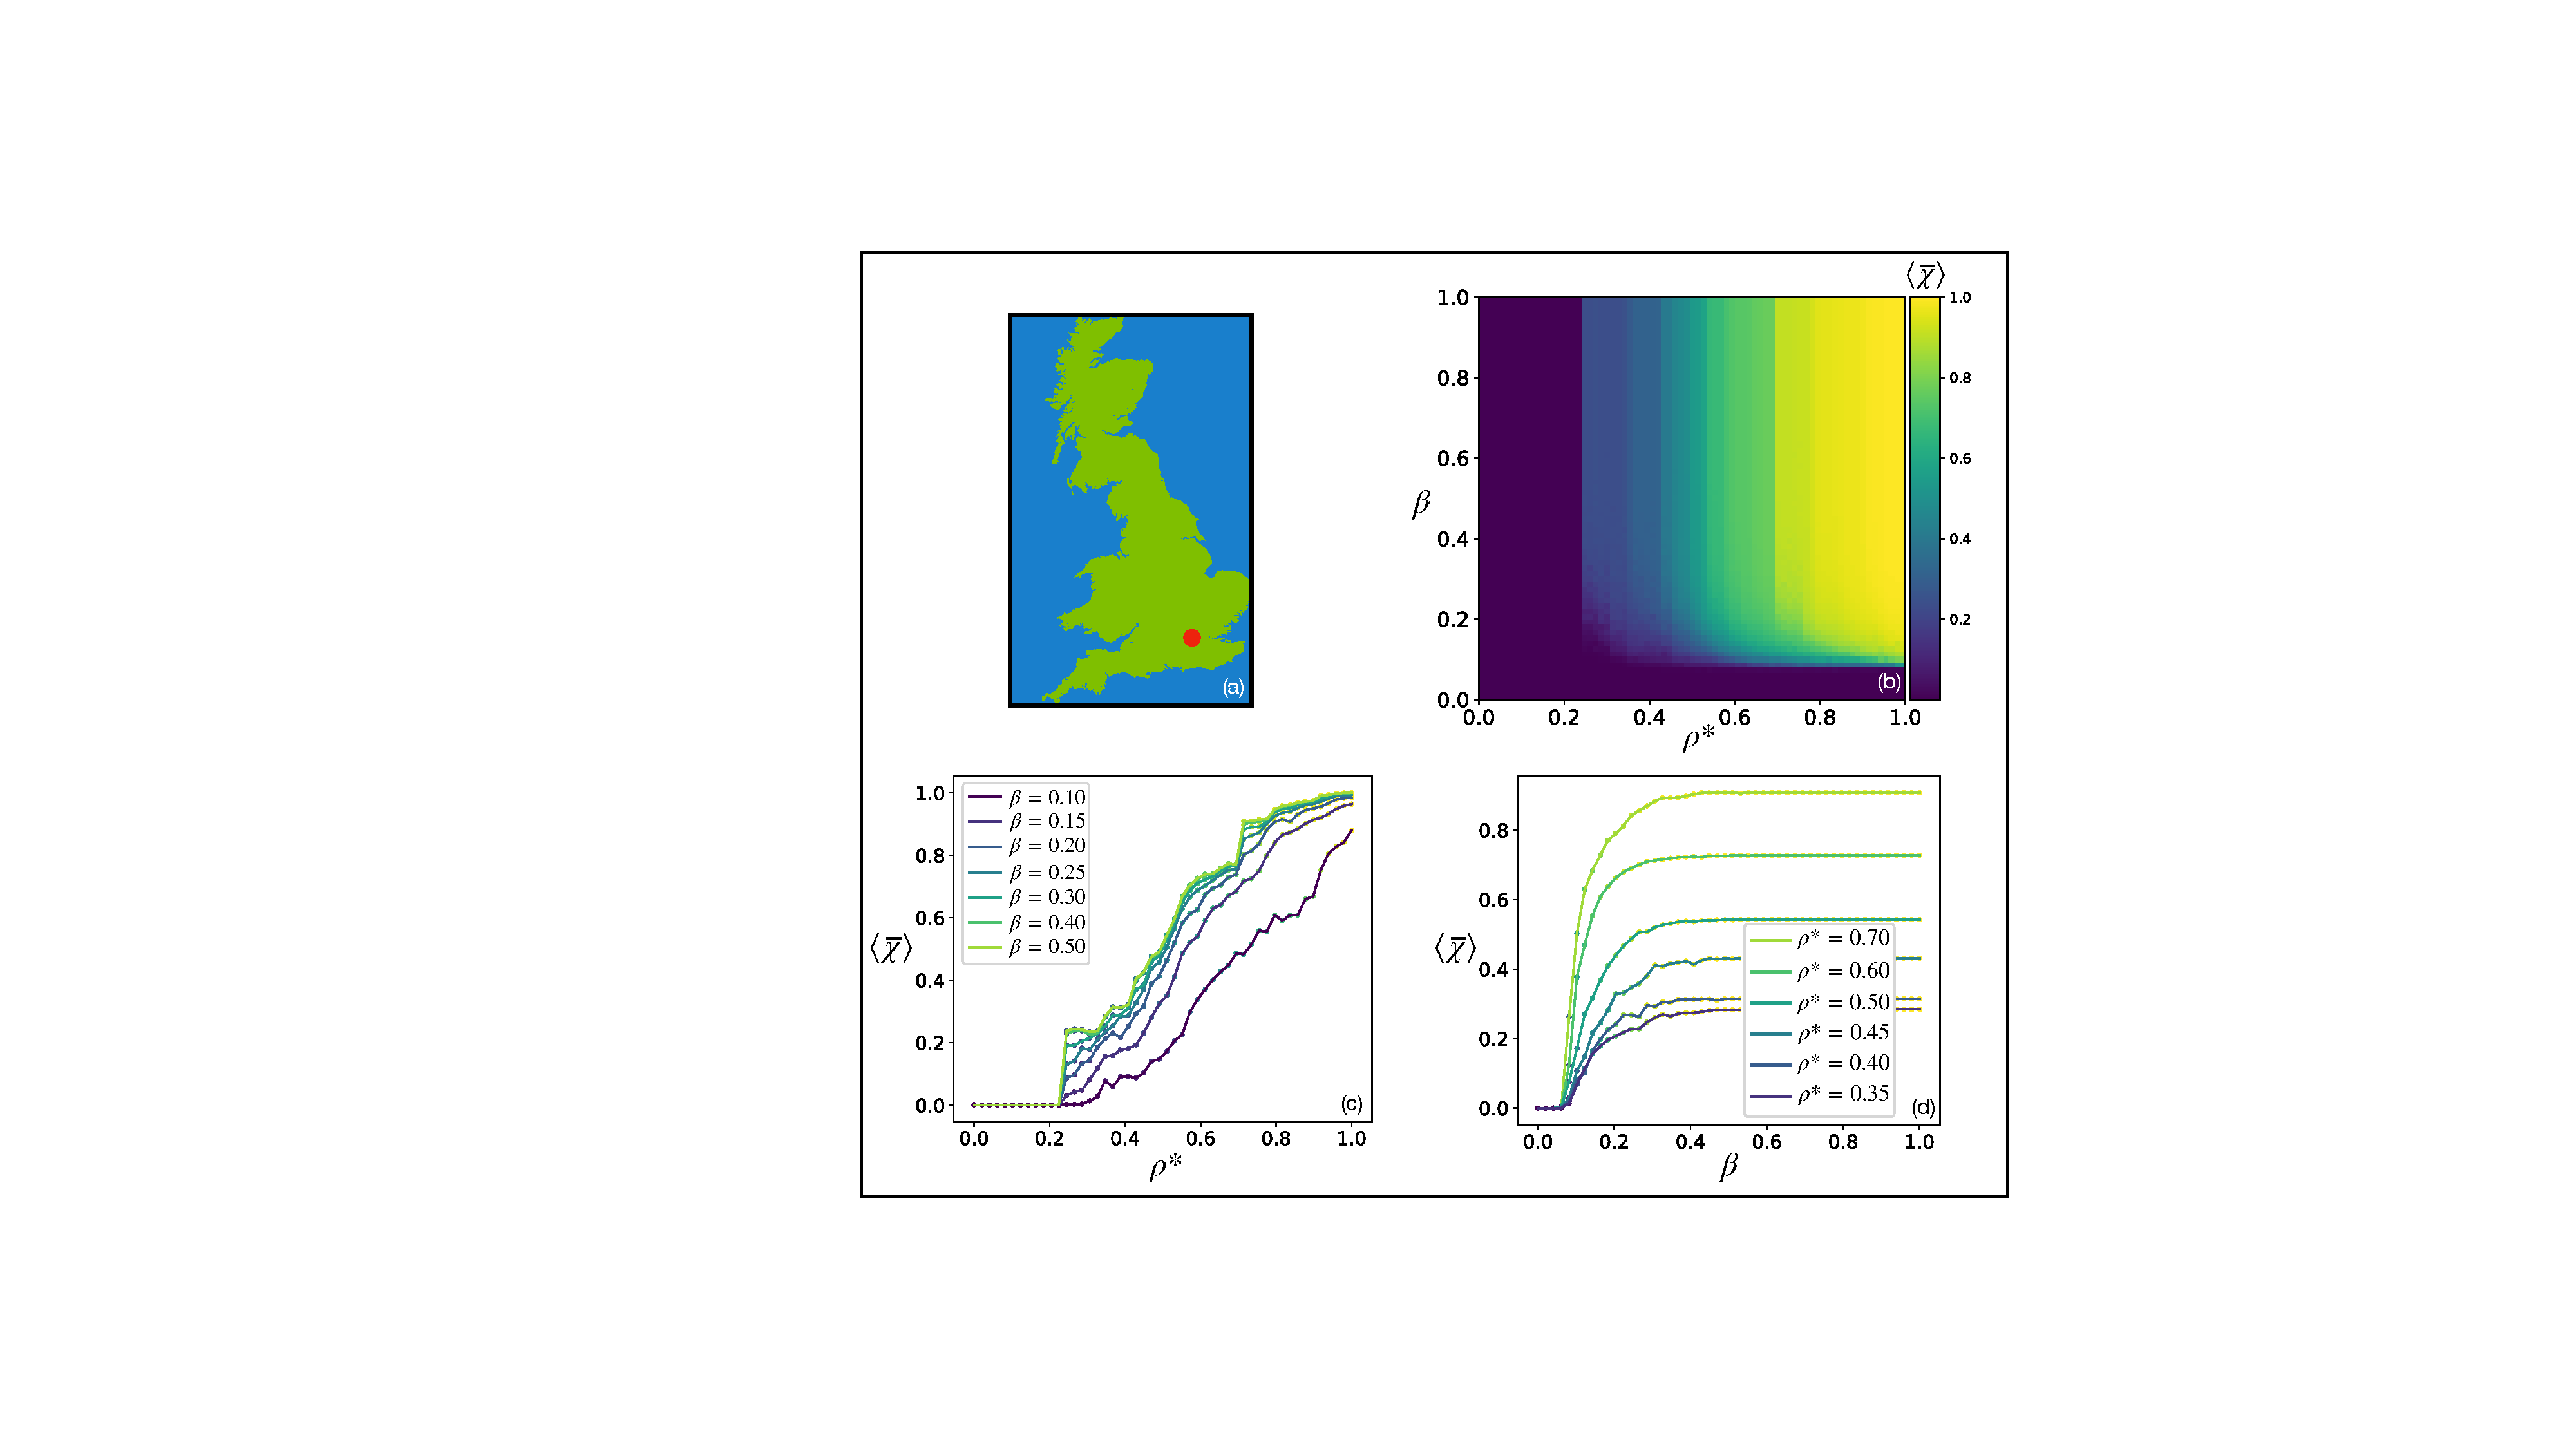
\includegraphics[scale=0.55]{chapter4/figures/figure4-param-sweeps.pdf}
    \caption{
    Beginning from a single fixed epicentre, shown in red inside panel (a),
    ensemble-averaged parameter sweeps of the toy model display a threshold-like behaviour.
    (b) The mortality ratio is plotted over the two-dimensional parameter space of $\rho^*$ and $\beta$. 
    (c) A one-dimensional plot of mortality as a function of host density is shown alongside several slices of infectivity, indicated by colour.
    (d) The mortality ratio is found over infectivity $\beta$ for different values of effective density $\rho^{*}$.
    }
    \label{fig:heterogeneous-phase-space}
\end{figure}

\newpage

\section{Discussion}

In this chapter, we explored two applications of the SLM viz; early warning signals and a toy landscape-level model.
The original analysis conducted by \cite{OROZCOFUENTES201912} relied on a velocity metric based on the number of 
infected and removed trees, $N_I$ and $N_R$ respectively. In this scheme, the number of infected and removed hosts scales as
$\propto (N_I + N_R)^2$ above the threshold, giving rise to an effective increase in velocity for later times;
as we discussed, these undesirable artefacts of domain geometry lead to confusing increases in the time series velocity, 
despite a constant rate of progression. Therefore, EWS were detected using an alternate (COM) time-series metric and abstract 
cylindrical domain configuration that negated geometrical effects.
A two-dimensional investigation was undertaken, sweeping the entire parameter space of tree density $\rho$ and infectivity $\beta$.

After setting up the EWS framework, the two-dimensional parameter sweep revealed that preemptive EWS detection is more obtainable 
when infectivity is lower. Observing these asymmetries in EWS detection, conditioned on infectivity
$\beta$, highlights the possible challenge of preempting progressively infectious pathogens;
in particular, given that host susceptibility is likely to increase as a consequence of climatic stressors \cite{garrett2006climate}.
Subsequently, we may hypothesise the heightened challenge of early warning indicator detection for forest-based pathosystems in the face of climate change.

EWS have found applications in a variety of ecological processes, 
e.g. aquatic ecosystem function \cite{kramer1991aquatic}, forest desertifications \cite{yang2005desertification}
and species-level extinctions \cite{drake2010early}.
Nevertheless, few sources focus explicitly on EWS from tree epidemics, akin to the dynamic (velocity-based) 
approach used by \cite{OROZCOFUENTES201912}. Instead, most research has focused on the more general class of forest
health and tree mortality\footnote{ 
See \cite{torres2021role} for a related review on remote sensing technologies and forest-health
} based on tree growth rings \cite{rogers2018detecting, mamet2015tree}. 
As such, the EWS method presented in section \ref{sec:EWS} differs from the wider literature,
and more work need to be done to scrutinise the utility of dynamic, velocity-based, EWS detection methods.

Secondly, we constructed a toy landscape-level SLM spreading through an example distribution oak, as generated by \cite{hill.data}.
The model of landscape-level epidemics neglects several essential features of invasive disease; most importantly, 
it inherited the nearest neighbour contact assumption, as discussed in chapter \ref{chapter:SLM}.
Hence, we labelled the landscape-level interpretation a`toy' model.
Although many limitations underpin the toy model (e.g. the omission of long-distance dispersal \cite{long-range-dispersal}
and cryptic infections \cite{gilligan2007impact}), it highlighted the inability of the SLM to describe the spread of disease
through lower tree densities ($\rho \in [0.01, 0.10]$), typical throughout GB.

As the SLM could not describe the spread of disease through more realistic host densities, 
we introduced an effective density parameter $\rho^*$, predicated on an arbitrarily chosen threshold.
Introducing an additional density threshold parameter is undesirable, unnatural and speculative.
Therefore, in the proceeding chapter, we are motivated to change direction and construct a non-local
dispersal model, in line with more contemporary dispersal-based approaches such as \cite{parnell2009optimal, meentemeyer2011epidemiological}.
In this paradigm, transmission between trees can occur over larger length scales and permit the spread over lower tree densities. 

Notwithstanding the inherent toy SLM shortcomings, its construction demonstrates the use of a novel modelled abundance
dataset provided by \cite{hill.data};
the modelled data is partly generated but combines various data sets\footnote{
Including ancient woodland shapefiles, BSBI distribution database, Countryside Survey data, myForest and the National Forest Inventory Great Britain 2014},
as we reviewed in section \ref{ch2:hostdata}.
However, statistically regressed (modelled) abundance data contains uncertainties and 
inaccuracies alongside the loss of small-scale host spatial structure $<1\mathrm{km^2}$.
As argued by \cite{13-challenges}, capturing host spatial structure, even when data are limited, 
is essential, and methods are required to assess the impact of incomplete or inaccurate host data.

Following this argument, host data accuracy presents a notable assumption in the toy model.
Be that as it may, density parameter sweeps over GB (as shown in Figure \ref{fig:heterogeneous-phase-space}) could 
form a simple procedure to assess the effect of host error, i.e. contrasting epidemic outcomes between two upper
and lower density error bounds. Evaluating landscape-level parameter-sweeps are uncommon, 
and most large-scale models repeat simulations over numerous control scenarios and rest on 
fitted parameters e.g. \cite{large-scale-control, doi:10.1111/j.1365-3059.2010.02391.x}.
Assessing disease outbreaks over a range of landscape-level densities parameters could describe a risk-based approach,
as articulated by some authors investigating epidemics through smaller spatial scales \cite{risk-potential-control}.

\newpage

% 5) Introducing non-local dispersal 

\section{Dispersal model: basic reproduction number}

As remarked in the opening chapters, the basic reproduction number is widely used in the %
study of epidemics in human and animal populations. %
The $R_0$ value is fundamental to understand the threshold of transmission, if $R_0>1$ the %
disease will spread through the population, or otherwise die out. The concept of $R_0$ is %
widely used, and misinterpreted \cite{delamater2019complexity}, and many different ways of %
calculating $R_0$ and available \cite{perspectives-on-r0}.\\

Various studies have considered $R_0$ for plant-based diseases %
\cite{gubbins2000population, park2001invasion, doi:10.1146/annurev.phyto.011108.135838, van2011periodic, mikaberidze2016invasiveness}. %
However, in the context of tree and plant-based epidemiology the concept remains far less %
explored. In general, $R_0$ is a complicated parameter which may vary in response to abiotic %
factors, such as temperature, humidity and wind-speed, or a changing contact network. %
When defining an $R_0$ value for tree-disease, the importance of spatial structure cannot be %
ignored \cite{park2001invasion}.\\

At the small scale we have a uniformly structured population. %
However, for larger scales there is considerable spatial heterogeneity. %
There fore, it is expected that some regions above the threshold host-density can support %
local reproduction of the pathogen, while some regions below the density-threshold cannot. %
Importantly, any measure of $R_0$ should separate these regimes with the threshold $R_0>1$. %
Infected regions are therefore likely to be `\textit{patchily}', distributed among the host %
population \cite{park2001invasion}.\\

Defining an informative $R_0$-value for tree-based pathosystems is far from simple. %
In particular, the value of $R_0$ will likely depend on the spatial scale we choose to %
consider \cite{mikaberidze2016invasiveness}. %
If  $R_0$ is measured over a small domain, we would under-count the number of secondary %
infections because long-range dispersal could infect a non-trivial amount of trees in %
neighbouring domains. %
Furthermore, a spatially-structured host population with dispersal-mediated interactions %
can expect to violate the \textit{well-mixed} population assumption\footnote{A spatially-dependant dispersal mechanism will limit the contact network and prevent the host population from being well-mixed}. 
Therefore care is needed in deciding how to define $R_0$.\\

\chapter{A non-local dispersal model}
\label{ch5:dispersal-model}

\subsection{Contact-tracing $R_0$}

An analytical solution to $R_0$ was presented previously in \textcolor{red}{CHAPTER 4}. %
In that approach, tertiary ($3^{rd}$ order generation) infections were not permitted. %
This allowed us to solely count the number of secondary infected trees due to the source infection. %
This is likely to over-estimate the number of secondary infections an infected tree could produce. %
Here, an alternate definition is presented that incorporates the effect of tertiary infections %
(up to $n^{th}$ order)  on the spatial structure.\\

Figure \ref{fig:contact-trace}(a) depicts a method, by computational means, of collecting $R_0$ %
through contact-tracing tree-to-tree interactions. %
At $t=0$ the primary infected tree, denoted by $A$, produces three $2^{nd}$ order infections %
$B$-$D$ shown in orange. %
The proceeding $3^{rd}$ order infections are shown in green, that is, $B$ infects $E$ and $F$ while $C$ infects $G$. %
Over the course of a simulation, the mean number of secondary infections produced by an $n^{nth}$ order infected tree is found. %
Doing so, leads to a generational mean denoted by $R^i_0$, an in this particular scenario $R^2_0=3$ and $R^3_0=1$. 
Throughout a simulation, a record is kept of all infection histories i.e. which tree infects which. 
To achieve this, trees are treated as particles in the sense that individual interactions between them are computed. 
This can be seen as equivalent to contact-tracing the resulting epidemic \cite{eames2003contact}. \\

For the remainder of this thesis, the basic reproduction number will be defined as $R_0=R^2_0$ unless otherwise stated. 
Defining $R_0$ in this way extends the previous definition to account for the realistic %
saturation around the primary infected trees neighbourhood. This gives an improved measure %
of the threshold for invasion.\\

\begin{figure}
    \centering
    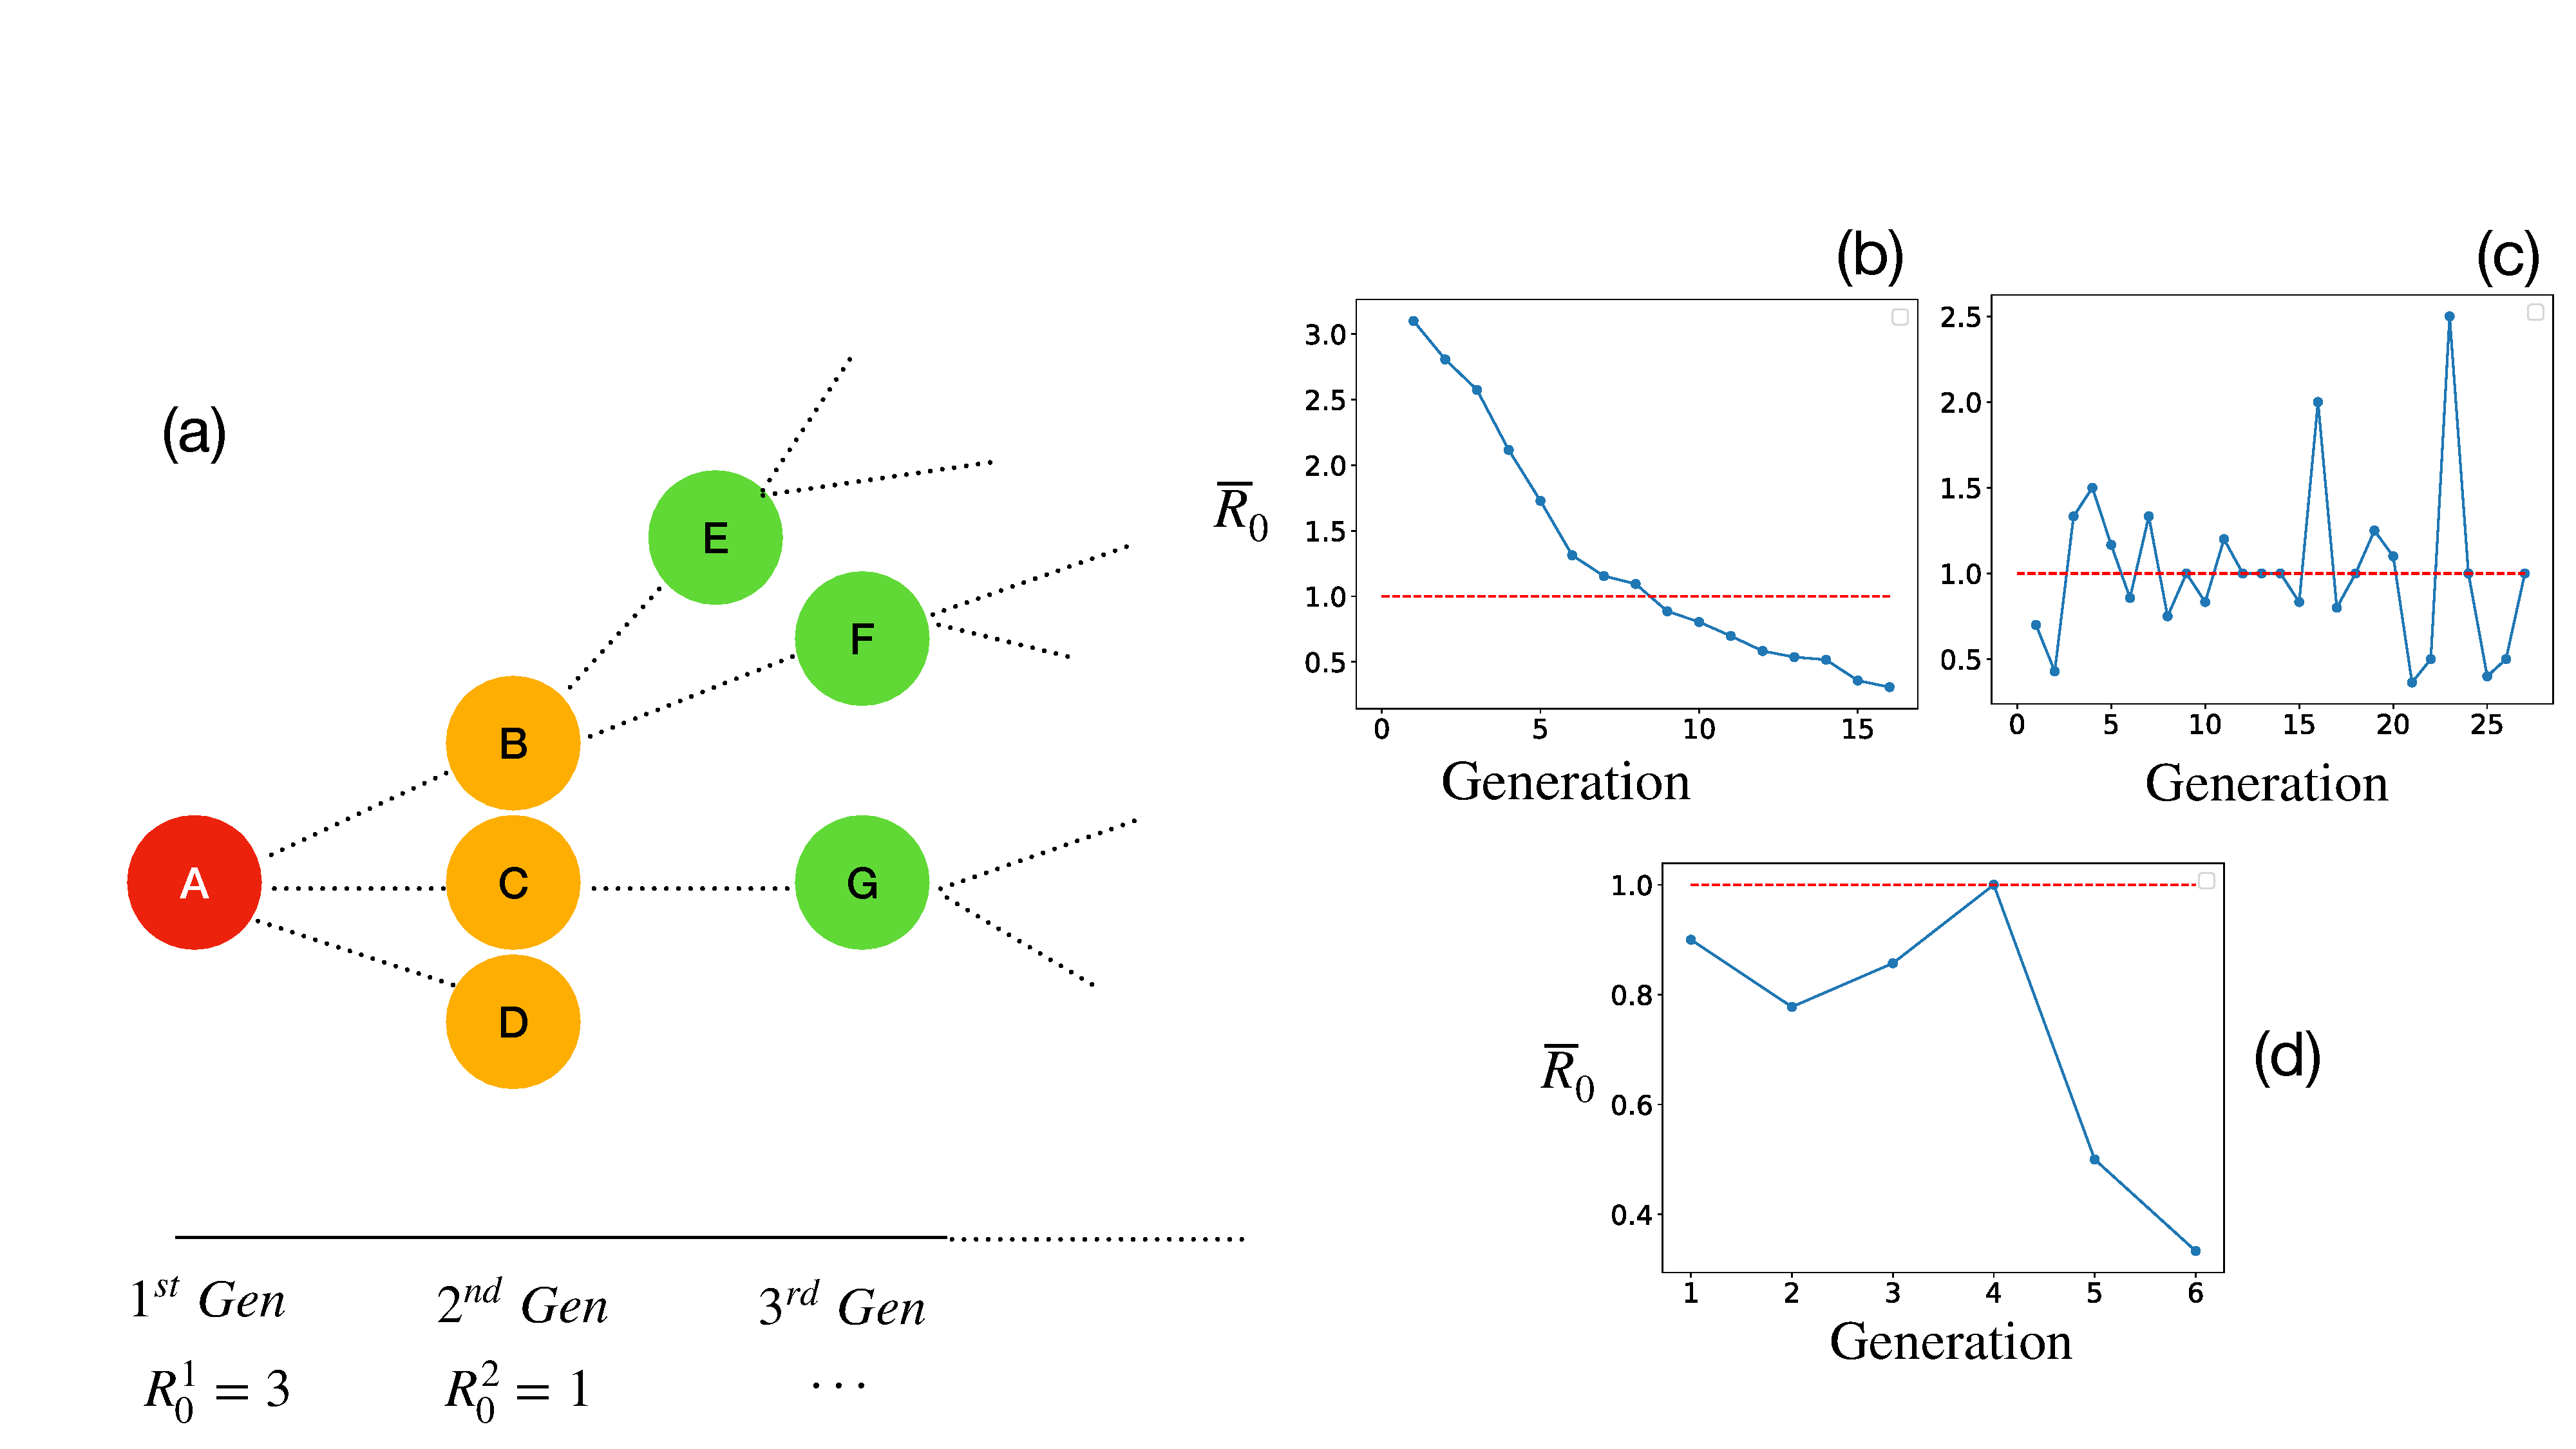
\includegraphics[scale=0.255]{chapter5/figures/fig1.pdf}
    \caption{Contact-traced $R_0$, the 'true' $R_0$. Tracking the history of all infected trees allows us to count how many infections are produced for each infectious tree over a simulation. At $t=0$, a single ($1^{st}$-generation) infection is positioned at the center of the domain. The quantity $R^i_0$ is defined as the mean number of infections produced for  the $i^{th}$ generation.}
    \label{fig:contact-trace}
\end{figure}


\subsection{Capturing $R_0$ in space and time}

In Figure \ref{fig:contact-trace}(b), we can see that measuring $R_0$ in a typical simulation, %
will likely over-estimate the contagiousness of the pathosystem at earlier times. %
Whereas, if $R_0$ is measured for later times (and the pathogen is above threshold), an %
under-estimate of the pathosystem contagiousness is likely. %
This is intuitive because the density of susceptible neighbors is higher at earlier times, %
on account of the neighborhood being untouched by other infected trees. %
The converse is true for later times in the simulation producing under-estimates. %
The number of secondary-infected trees will thus vary over time\footnote{Variations can %
also be expected at different locations through the domain. That is, centrally-distributed %
trees would, in theory, have access to infected more susceptible neighboring than trees %
located on the edge of the domain.}. %

Figure \ref{fig:contact-trace}(c) reveals how the pathosystem can behave if the threshold for %
invasion is just satisfied. %
Here $R_0$ is just above threshold for earlier times and barely spreads, however, the spread is chaotic. %
This can be considered a non-local generalisation of the SLM spreading on the critical point. %
In this scenario, $R_0$ is not strongly dependant on time. %
In the below-threshold regime, $R_0$ remains below $1$ for all generations and dies out after %
two generations. %

From Figures \ref{fig:contact-trace}(b-d), we have demonstrated that this definition of $R_0$ %
reliably captures the threshold of transmission during the initial stage of infection. %
Undesirably, we have made simplification in the assumptions and have not achieved a complete %
characterisation of $R_0$\textemdash which could, in be defined in terms of a growth %
rate per generation \cite{R0-construct}. %

We have not considered the re-growth of susceptible trees. %
If the number of susceptible hosts is fixed, without replacement, the number of susceptible hosts %
will continually decrease in time if an epidemic takes hold. %
This will reduce $R_0$ drastically for later time-periods. %
It appears inescapable that tree and plant-based systems violate the well-mixed population %
assumption that classic definitions of $R_0$ are based on. %
\textcolor{red}{Investigate how the next generation operator is used in the literature.}\\

% Averaging R0 over the entire ensemble will reduce R0, thus flatten the R0 map and reduce the amount of spatial clustering we see -- could illustrate this with a figure.

\subsection{$R_0$ and spatial scale}

Given that we have now defined $R_0$, we will investigate how this quantity changes in relation %
to the parameters dictating the spatial scale in our model. %
The parameters of interest are domain size $L$ and scale parameter $\alpha$. %
The domain size $L$ controls the array dimension stored in  memory, while $\alpha$ %
describes the physical space per-point inside the array i.e. the model resolution. %
The number of infections produced for each generation, $R_0^i$, were ensemble averaged with %
different values of domain size $L$ and scale parameter $\alpha$, %
shown in Figure \ref{fig:R0-spatial-scale}. Simulations started with a single infected, %
primary source, tree at the center of the domain and continued until the primary source %
transitioned into $I\rightarrow R$. %
The final number of contact-traced secondary infections produced from the primary infection %
constitute $R_0$.\\

The scale parameter of $5\mathrm{m}$, together with $L$, describe a range of different modelled %
areas which could represent fields, forests, stands or patches of land etc\footnote{Throughout this chapter, %
we take the domain to represent the average density of trees through a landscape.}. %
In Figure \ref{fig:R0-spatial-scale}(a), we can see values of $R_0^i$ increase with $L$ and %
begin to saturate to constant levels with a domain size $L\times L=1000\times 1000$, or $5\mathrm{km}\times 5 \mathrm{km}$. %
Beyond which, changes in domain size had negligible effects on $R_0$. %
This suggests for domain-sizes, up to some limit, the invasiveness of the pathogen has a %
dependence on the domain-size within which we choose to measure the spread. %
The result of Figure \ref{fig:R0-spatial-scale}(a) falls nicely in line with the work of %
others \cite{mikaberidze2016invasiveness} and suggests that the spatial scale is likely to %
alter the threshold of invasion.\\

The result of Figure \ref{fig:R0-spatial-scale}(a) is intuitive. %
Suppose we decide to calculate $R_0$ for a \textit{small} patch of land at density $\rho$, %
given a number of infected trees. In the case of wind-dispersal, it is clear to see that some %
innoculum (e.g. spores) would disperse out of the patch of land and infect other trees in %
neighbouring patches we are not considering. The value of $R_0$ is therefore subject to %
under-estimation for domain sizes small in comparison to the scale of dispersal.\\ 

On the other hand, suppose we measure $R_0$ for a larger patch of land at the same density $\rho$. Here, it is clear to see that we would count more secondary infections per infected tree and therefore measure a higher value of $R_0$. That is, the majority of dispersed inoculum will now land inside the domain boundary and directly effect the trees we are considering. At some point increasing the domain size will have no effect on $R_0$. This is likely to occur when the amount of inoculum, produced per tree\footnote{In our case $\beta$ represents a simplified compound parameter incorporating the amount of spores produced per tree and the probability of spore uptake by another $S$-tree.}, saturates the domain with only negligible amount of dispersing out of the patch.\\

\begin{figure}
    \centering
    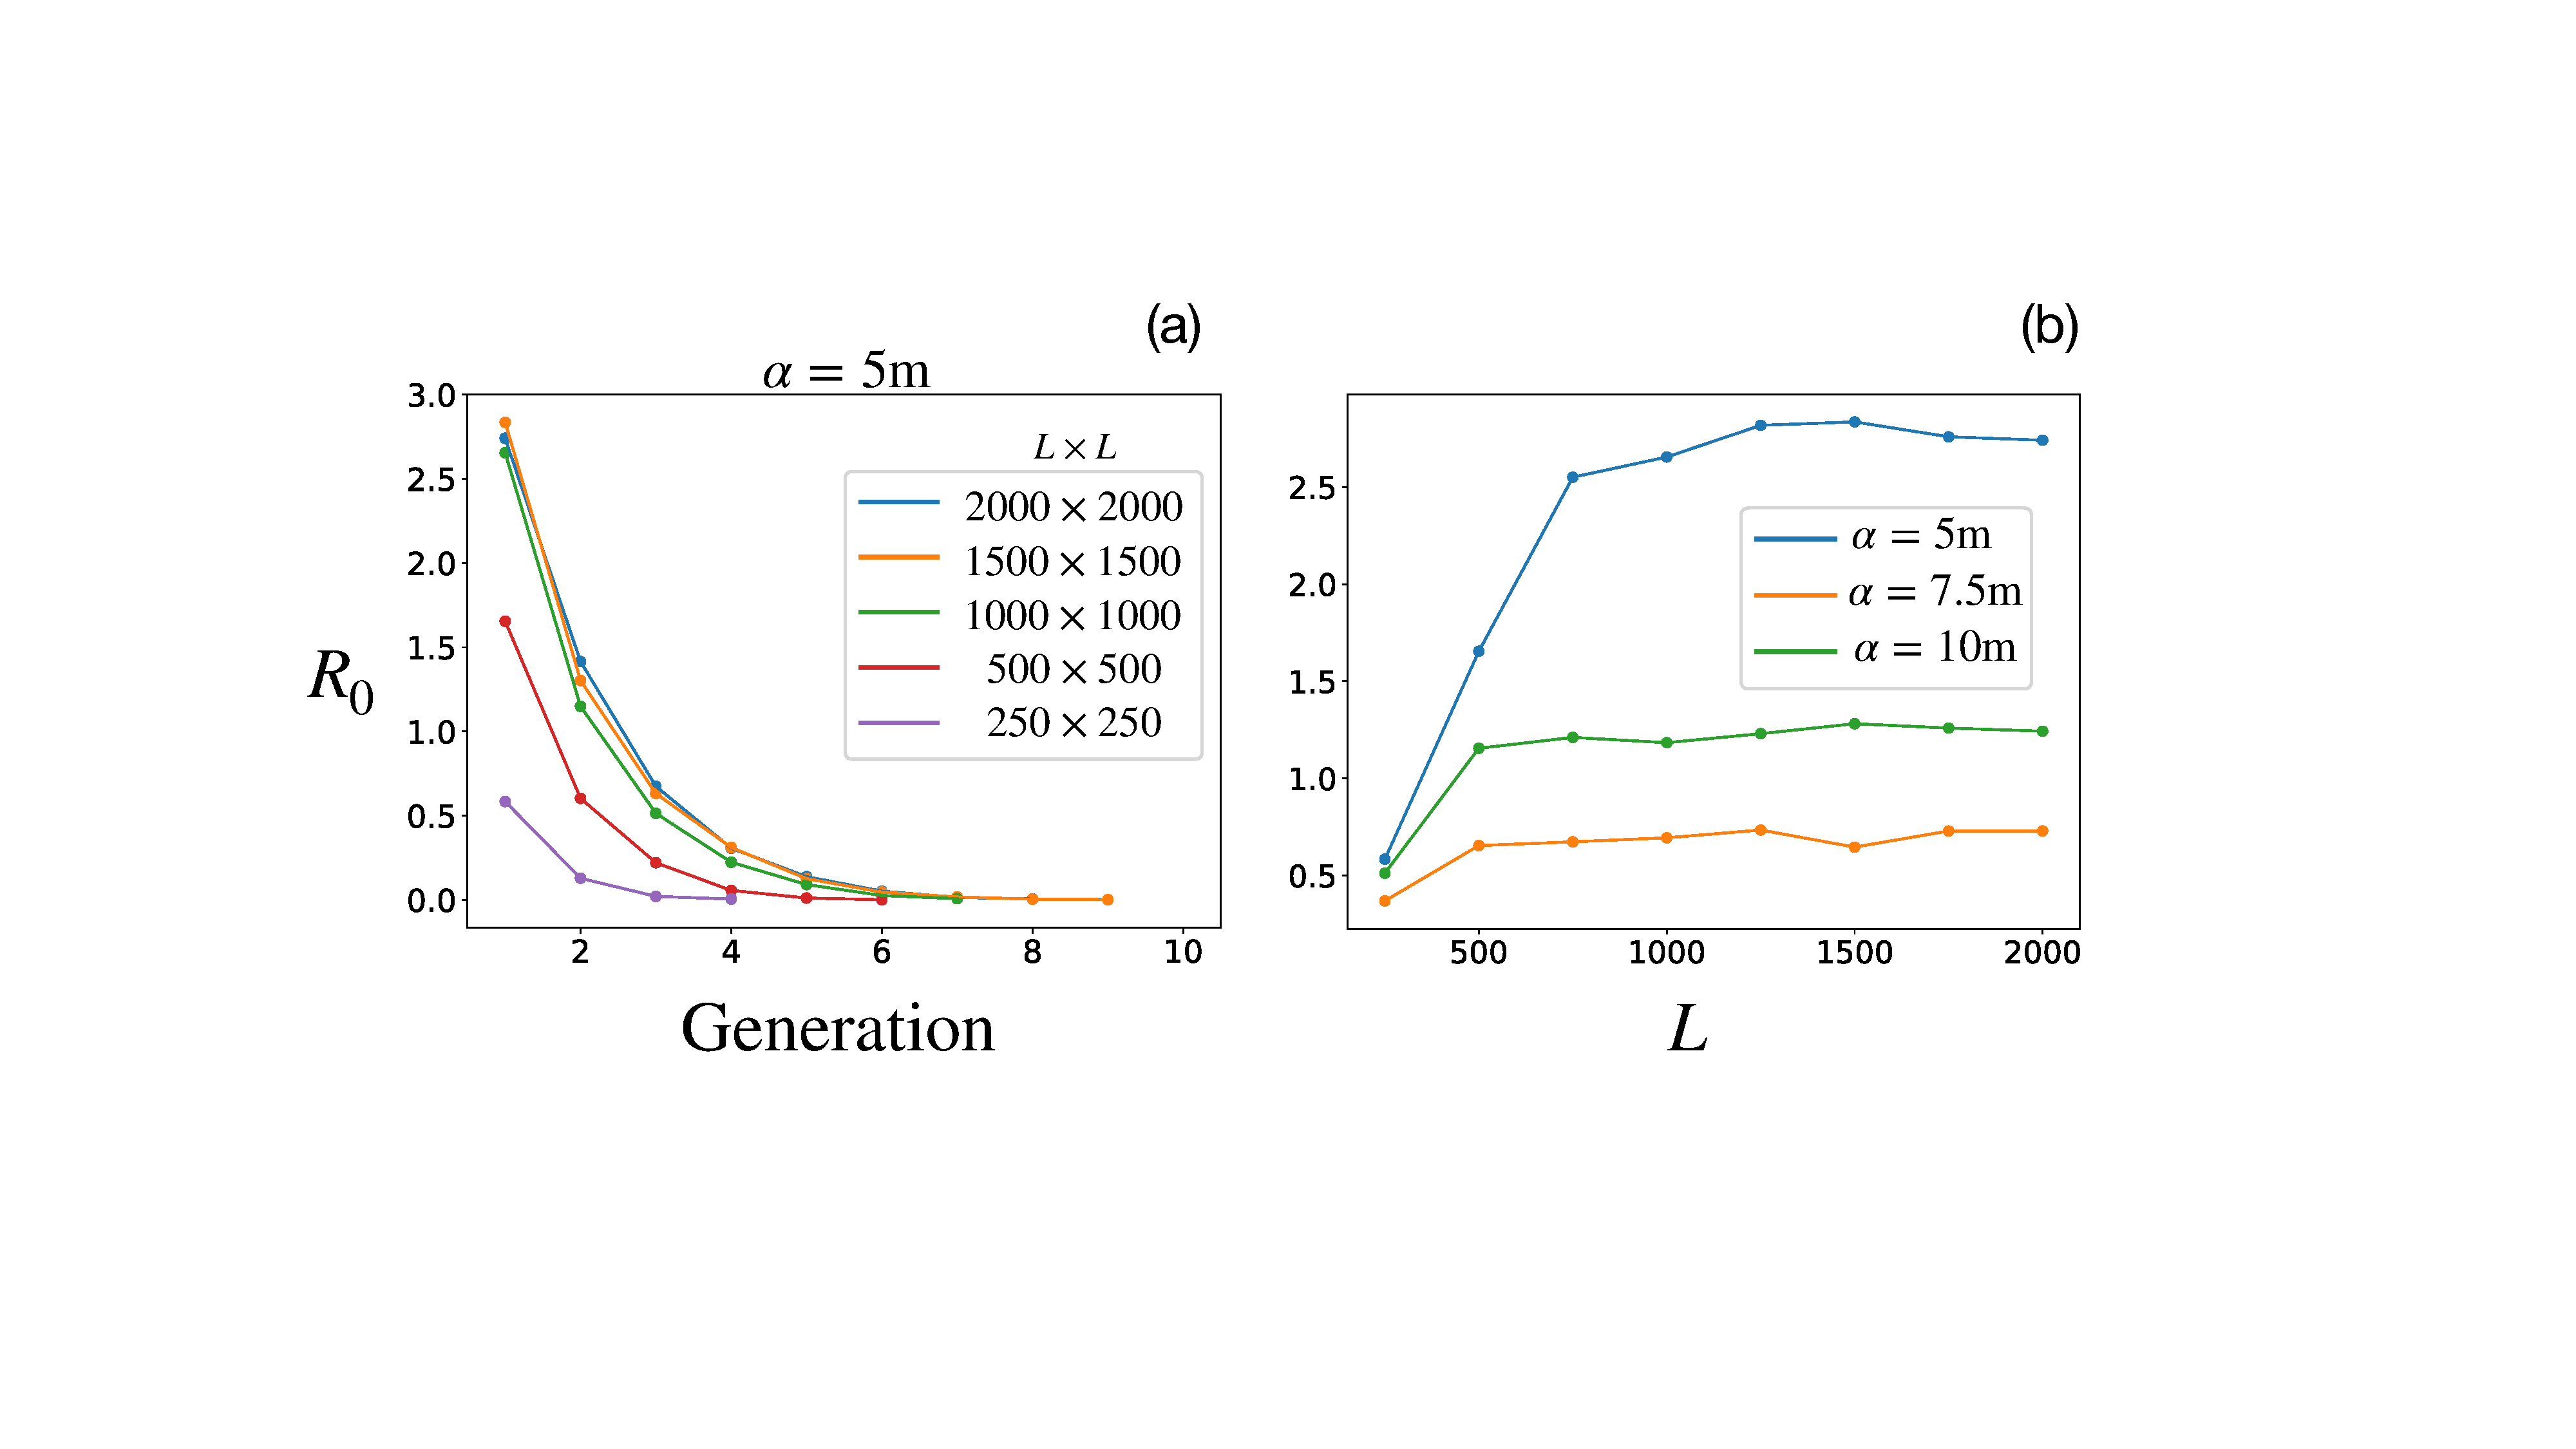
\includegraphics[scale=0.3]{chapter5/figures/fig2.pdf}
    \caption{How $R_0$ depends on scale...}
    \label{fig:R0-spatial-scale}
\end{figure}

Figure \ref{fig:R0-spatial-scale}(b) shows the model behaviour when the scale parameter is %
changed in conjunction with the domain size $L$. From this we notice a drastic and surprising %
reduction in the scale of pathogen spread for higher $\alpha$. %
This points towards a limitation in our model infectivity parameter $\beta$. %
Increasing $\alpha$ has the effect of increasing the average spacing between trees and %
increasing effective host canopy cover. %
In changing $\alpha$, the spatial resolution is rescaled and the expectation is that a higher value of $\beta$ should be seen to reflected a larger canopy cover. %
The infectivity $\beta$ represents a simplified compound parameter that incorporates information about the spore production rate. %
Re-scaling the canopy cover means more susceptible plant material can become infected and produce further spores. 
% JS_what does this mean 
\textcolor{red}{Tighten me up, talk about me to group.}\\

% 6) A method of control at the landscape level 
\chapter{Regionally Containing Epidemics: Modelling Ash dieback}

% paper title: Large-scale control based on regional containment
% there is a surprising lack of, simplified, ash dieback models in the literature...\ciations... <-- double, triple and quadruple check!
% without host demography 
% landscape level control strategy

Previously in Chapter \ref{ch5:dispersal-model}, we considered a generic $SIR$ dispersal model that spread via wind. Constructing the dispersal model resolved the major problem witnessed in Chapter \ref{fig:ch4_uk_spread}, namely, the failure of the SLM to spread on a realistic host density. However, the findings of Chapter \ref{ch5:dispersal-model} lacked biological specificity and thus, came short of aiding plant health. The present chapter aims to address this by constructing a landscape-level control strategy on a simplified model of ash dieback ADB. The control strategy is largely generic, and could in principle be adapted for any wind-borne tree disease.

There has been a great deal of work carried out into the nature of control in plant and tree-based epidemics\footnote{See section \ref{chapter2:plant-ecologoy} for a review on the control in plant-based epidemics.}. In particular, the spatial structure of plant-hosts is an essential factor when considering how to manage an outbreak \cite{spatial-control-optimisation, control-heterogeneous-landscapes}. The accepted paradigm of control typically considers infected tree removals over a relatively small spatial scale, near infected hosts \cite{WEBIDEMICS}, or more broadly, ahead of the wavefront \cite{large-scale-control}. However, landscape-level epidemic control, based solely on the structure of large-scale spatial distribution of hosts incorporating topography, has yet to be explored in-depth.\\

As such, in this chapter, we will examine how host-heterogeneity, under the influence of a wind-dispersed pathogen, can give rise to natural pinch-points and fault lines in the spatial distribution of hosts. Population pinch points may give rise to a bottleneck in the epidemic spread, which in principle, may be exploited with targeted tree felling to fragment the host population with minimised effort. In essence, a strategy of 'regional containment', targeting the local wind-based pathogen dispersal mechanism, is formulated and scaled up over large spatial scales. Similar concepts for crop and livestock diseases have been outlined \cite{PAPAIX201435, GILIOLI20131, Gilligan-disease-management}, however, to our knowledge, this has not been generalised to tree population distributions over large spatial scales.

A simplified $SEIR$-type model of ash dieback is developed to demonstrate this control strategy, alongside an appropriate definition of the reproductive ratio\textemdash denoted by $R_0$. The value of $R_0$ is projected onto the map of ash tree canopy cover in GB, as given by \cite{hill.data}. From the $R_0$ maps we construct, a simple notion of epidemiological connectivity can be defined and visualised through a susceptible '$R_0$-cluster' over the population of GB ash trees. This leads us to develop a heuristically-based fragmentation algorithm. As we define it, fragmentation considers which locations in the population, if artificially taken below $R_0 = 1$ through felling, would disrupt epidemiological connectivity\textemdash, thus leading to containment. Epidemic containment in the largest $R_0$-cluster is then analysed and shown to be most applicable over a specific range of infectivity parameters.

It is widely accepted that ADB will wipe out the vast majority of ash in Great Britain over the next few decades \cite{ash-dieback-costs}. Therefore, large-scale control efforts aim to slow the spread, in contrast, to complete containment. % Find references of current efforts/guidelines 
A slower rate of spread benefits ash populations allowing them to recover alongside artificial replanting.% reference 
Although the strategy of control presented in this chapter is demonstrated on a simplifed model of ADB, the results are generic and could be applied to any wind-dispersed pathogen.
The pathosystem ADB presents an interesting and relevant case study of an emerging epidemic whose reproductive mode is both seasonal and subject to LDD. The]refore, a model of ADB brings together the several key elements of chapter \ref{ch5:dispersal-model}, measuring $R_0$ over different temporal and spatial scales. 

The challenge of controlling ADB primarily reflects the challenge of containing a pathogen that spreads via long-distance dispersal (LDD). As such, developing a landscape-level control strategy when there is LDD (and epidemic uncertainty) present several obstacles that must be acknowledged beforehand. Firstly, the complexity of modelling ADB is a thesis in and of itself, few parameters are known, spatial and genetic variations are significant \cite{stocks2017first, mckinney2014ash} and a dependency on the landscape \cite{doi:10.1111/1365-2745.13383}. Moreover, HP can infect ash through diverse mechanisms such as water-course and contaminated soil and LDD means that new and distant foci can emerge over large distances without the need for nearby ash\textemdash for a more detailed review of ADB, including the challenges of control and biology, see chapter \ref{chapter2:litrevieiw}.

multi-scale approaches have been outlined \cite{hart2020theoretical}
multi-seasonal frameworks comprise a common theme in the spread of crop-based epidemics see  x, y, and typically involve soil-borne nematodes-based outbreaks \cite{tankam2020modelling} <- see references inside.
ash dieback has a strong morality rate \cite{stocks2017first}

\section{Constructing an $SEIR$ model}

\subsection{On the biology of ash dieback}

The primary infection mechanism occurs when the fungal spores of \textit{H.pseudoalbidus} (HP) are wind-dispersed in the summer and land on the leaves of susceptible ash. Once the pathogen colonises a leaf, it spreads to the xylem and then throughout the whole tree. % references on mechanism
An infected tree will then shed its leaves in the autumn. Fungal fruiting bodies then grow on dead leaf litter until summertime; at that point, spores produced by the fruiting body are wind-dispersed and continue the cycle by producing new secondary infections.% expand on the fruiting body spore production.

Specific to ADB, there are two stages of dispersal: the causal agent HP is dispersed on infected leaves during the yearly shed of ash, secondly, wind dispersal of fungal spores. Fortunately, the aggregate behaviour of two-stage dispersal is captured by sampling the amount of fungal spores with distance from a nearby source of infected ash \cite{grosdidier2018tracking}\textemdash discussed more below. 
Be that as it may, an infected tree is treated as the dispersal site in the model, although the realistic description is not so simple.

The life cycle can be understood to have two phases of growth, sexual and asexual. % reference
The asexual phase occurs when the pathogen infects and amplifies through the host \textcolor{red}{and occurs all year round}. The sexual phase of HP occurs during the summer months, from June until September when wind-dispersed spores infect new ash trees. % double check the red-highlighted

The seasonal infection cycle of ADB resembles that of crop-based disease \cite{tankam2020modelling}. Although, in the context of crop disease, removal usually coincides with harvest time. In contrast, ash infected with HP can be removed by the pathogen over a time frame spanning years. Once infected, the time ash survive depends on a plethora of factors such as age, surrounding landscape, genetic susceptibility or the particular mode of pathogen infection\footnote{For example, the pathogen can colonise the root-system \cite{schumacher2011general}, usually in severely infected ash \cite{https://doi.org/10.1111/mpp.12073}. From this point, it is only a matter of time before opportunistic fungi invade and significantly accelerate mortality \cite{enderle2013temporal}.}. In Germany, a forest stand of planted ash trees had a $73\%$ mortality rate after five years \cite{langer2015ash} (as cited in a review \cite{enderle2017ash}), while observations of ADB progression in Austria suggest a low mortality rate of $5\%$ measured over a two-year window \cite{kessler2012dieback}. Furthermore, a study conducted at different sites throughout England suggests a time-scale ranging between $3-15$ years of infected tree growth before death \cite{wylder2018evidence}.

% The mortality of infected ash infected with HP is high, recent estimates suggest around $95\%$ \cite{stocks2017first}. % check \cite{ash-dieback-costs} paper for other estimates

\subsection{Infection dynamics}
\label{sec:infection-dynamics}

\begin{table}[h]
\centering
\begin{tabular}{l l l}
\hline
\textbf{Model parameter} & \textbf{Description} & \textbf{Value(s) taken}\\
\hline
$\rho$  & Tree density & $0.00 - 0.10$ \\ 
$\beta$ & Infectivity & $0.00010 - 0.00100$ \\
$\ell_{ga}$ & Gaussian dispersal scale parameter& $196\mathrm{m}$ \\
$\ell_{pl}$ & Power-law dispersal scale parameter& $203\mathrm{m}$ \\
$a$ & Power-law dispersal exponent & $3.3$ \\
$T$ & Sporulation peak & June - September \\
$t$ & Time-step & $1\ \mathrm{day}$\\
$R_0$ & Mean reproduction number & $0-20$ \\
$\mathcal{L}$ & Lattice dimension & $1000\times1000$ \\
$\mathcal{A}$ & Domain area & $5\mathrm{km}\times5\mathrm{km}$ \\
$\gamma$ & Lattice constant & $5\mathrm{m}$ \\
$\mu$ & Peak leaf-shedding of ash & November \\
$\sigma$ & Leaf-shedding standard deviations & 2 weeks \\
$\lambda$ & Mean exponentially-distributed infectious life-time  & $5\ \mathrm{years}$ \\
\hline
\end{tabular}
\caption{Parameters used in the $SEIR$ model of ash dieback. The dispersal parameters are taken from \cite{grosdidier2018tracking} and the typical tree densities of ash are informed from by \cite{hill.data}.}
\label{tab:SEIR-model}
\end{table}

As before, the hosts' distribution, in this case ash, is initialised by a Bernoulli trial with probability $\rho$ according to a binomial distribution\textemdash thus giving rise to a flat and randomly distributed landscape of trees. The probability $\rho$ defines the host density inside a square domain of size $\mathcal{L}$. Each lattice point is chosen to represent a $5\mathrm{m}\times5\mathrm{m}$ patch of land that approximates the canopy cover of an ash tree, this resolution yields an upper bound of $400$ ash trees per hectare of canopy cover \cite{ash-tree2, ash-tree1}.

However, this time, we include an extra latently infected (or exposed) compartment, denoted by $E$, into the model. Thus, a tree can be in one of four compartments and transition through $S\rightarrow E \rightarrow I \rightarrow R$, without the possibility of recovery. Figure \ref{fig:SEIR-transitions} shows a typical scenario; an infected ash tree in the $n^{th}$ cycle, or equivalently $n$ years after the initial outbreak, may infect ash in the $S$ compartment. Newly infected ash will transition into the $n^{th}$ $E$ compartment, denoted by $E_n$, and become infectious in the following year $I_{n+1}$. 

In the $E$ compartment, trees are infected but not infectious. Additionally, the compartments $(E_1, E_n,..,E_n)$ do not represent different biological states. The index $n$ is included for convenience to highlight the fact that latently infected ash take, on average, one year before producing new secondary infections.

\begin{figure}
    \centering
    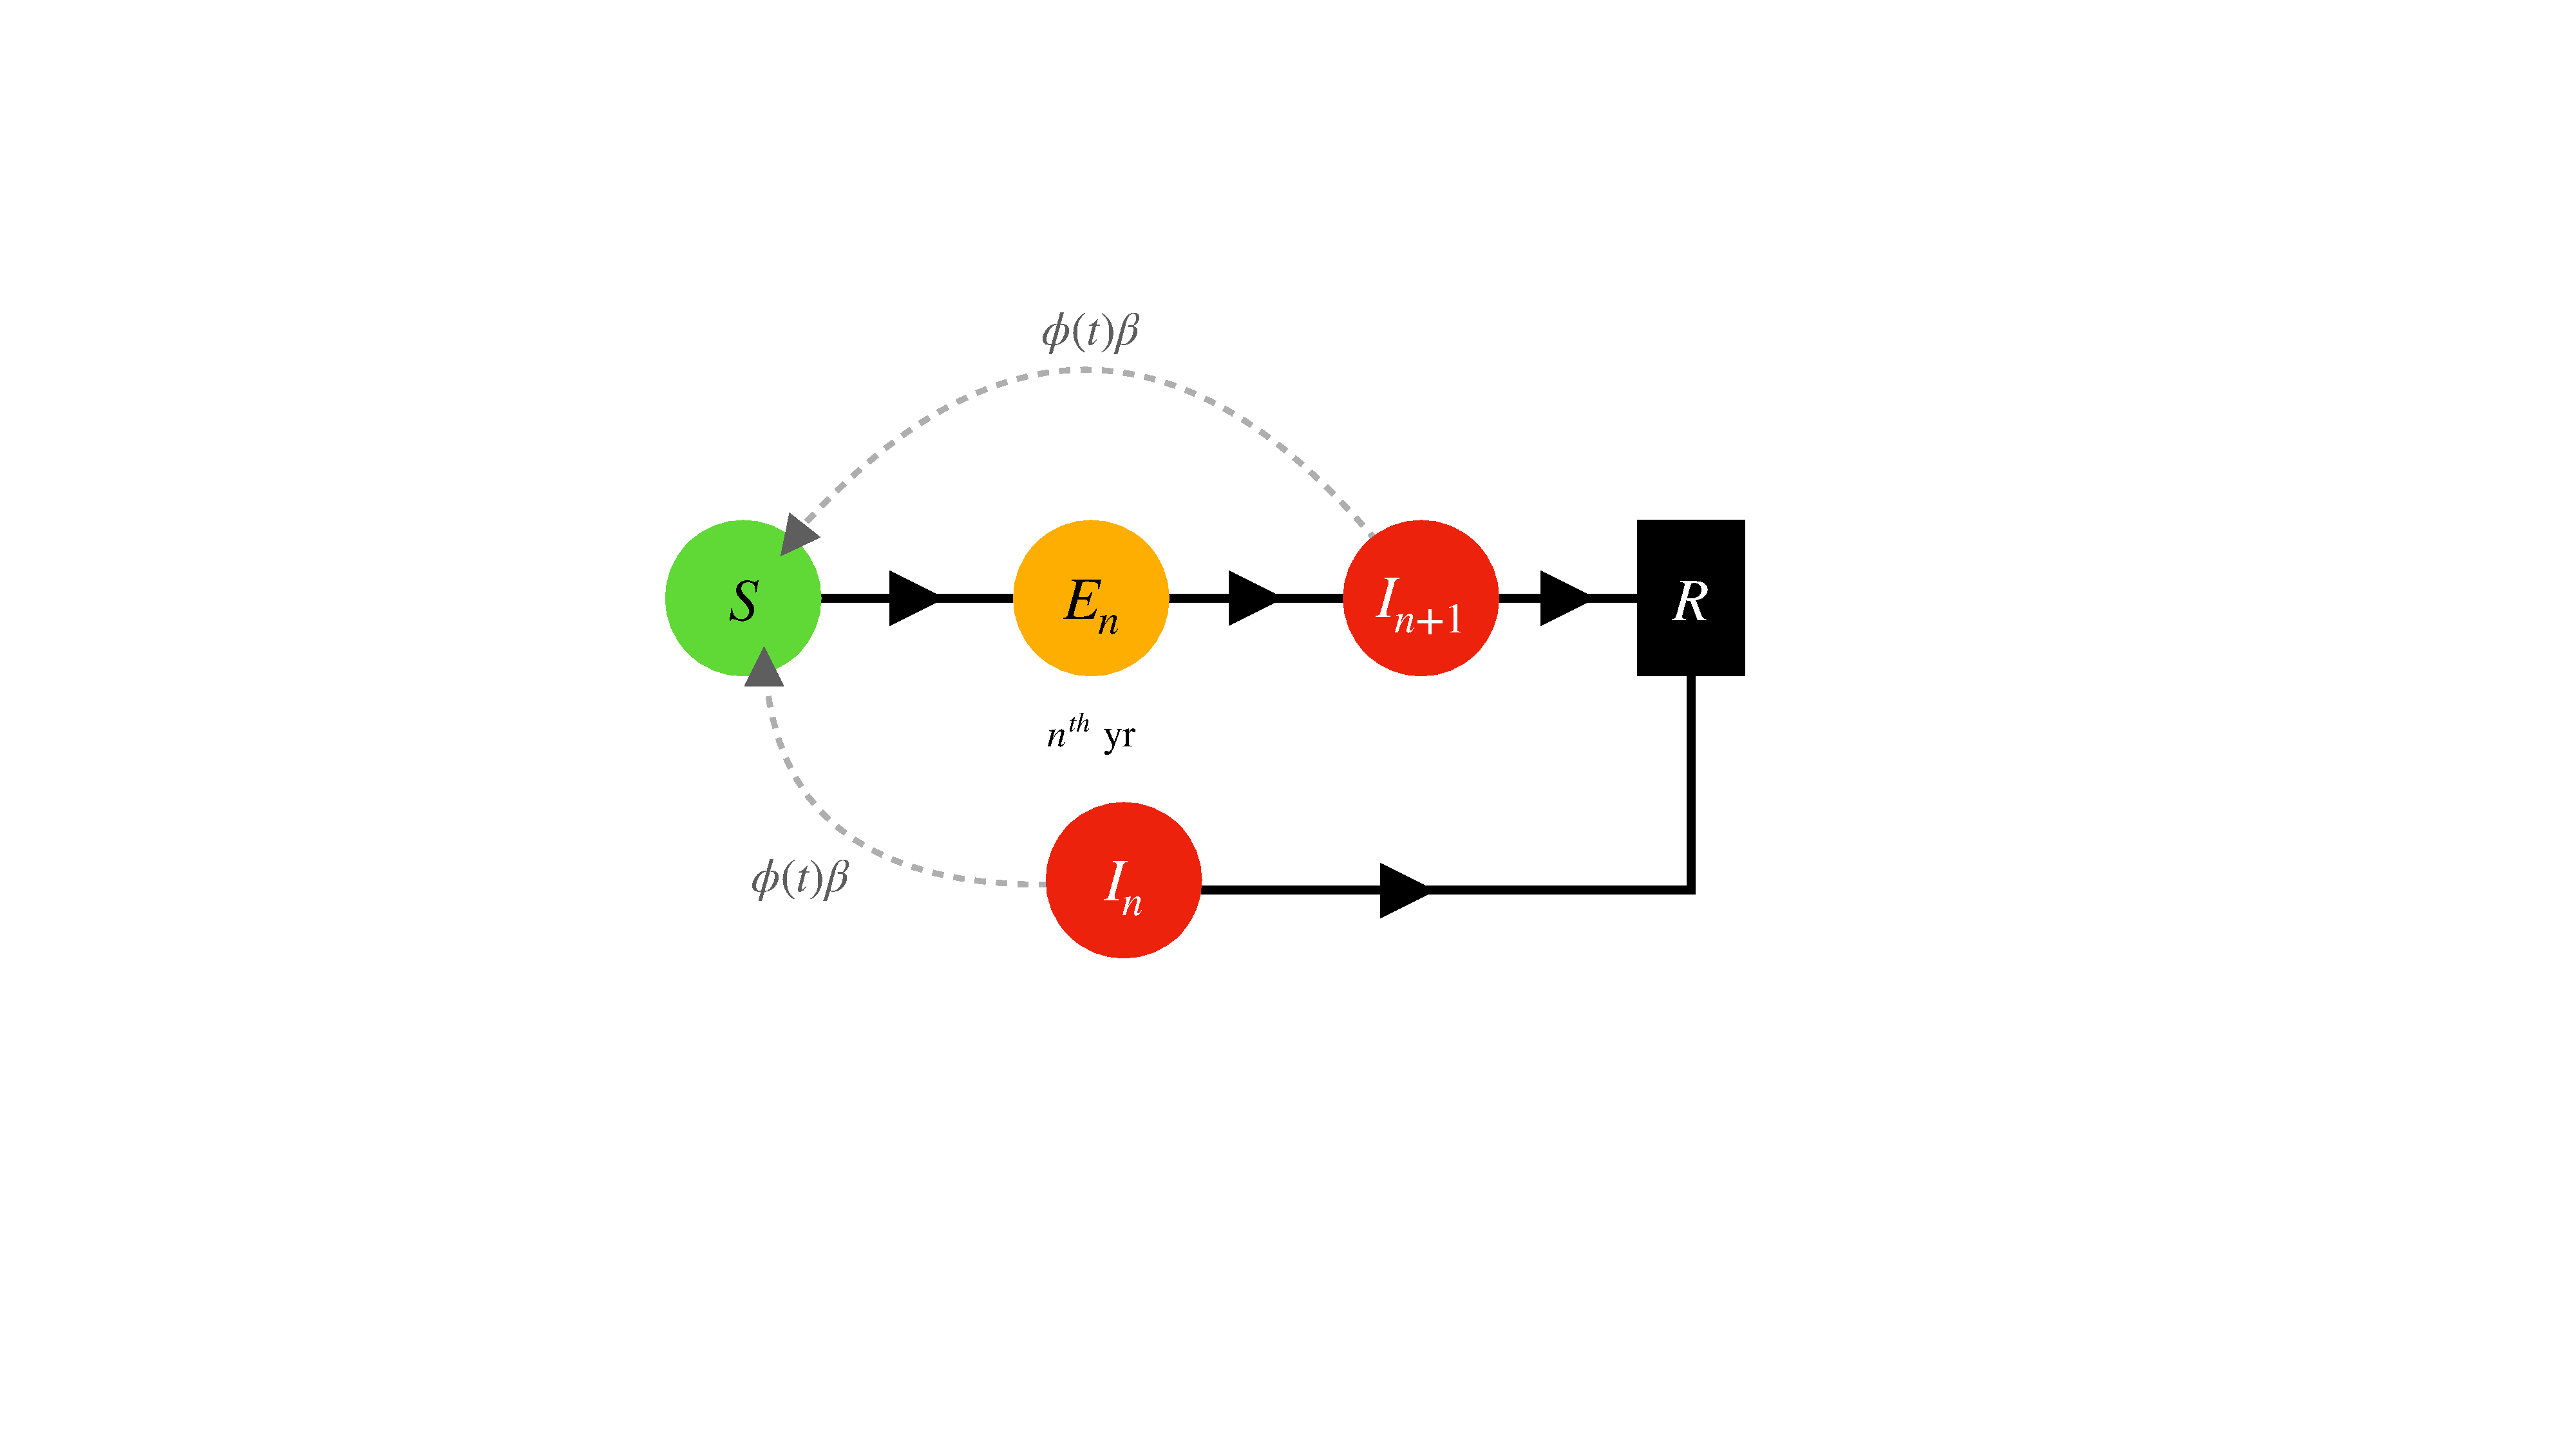
\includegraphics[scale=0.30]{chapter6/figures/fig1.pdf}
    \caption{The $SEIR$ model of ash dieback. In year $n$ of an outbreak, an infectious tree may cause a transition $S\rightarrow E_n$, depicted by the bottom dashed grey arrow. A tree that becomes latently infected in year $n$ will lead to an infectious tree in year $n+1$. Eventually, all infected ash are removed without the possibility of recovery.}
    \label{fig:SEIR-transitions}
\end{figure}

As defined here, an ash tree transitions into the infectious compartment when leaf shedding begins in Autumn. A Gaussian distribution centred in November with a two-week standard deviation represents this in the model. This particular choice of standard deviation, although best-estimated, is ultimately ill-informed. However, because infected ash do not produce any secondary infections until the following summer, we can afford some degree of flexibility modelling the exact timing of transitions between $E_{n}\rightarrow I_{n+1}$; this flexibility is demonstrated in-depth later on.

Once in the infectious compartment, an infected ash tree will not give rise to any secondary infections until summer when fruiting bodies produce their spores on dead leaf litter. Thus, infectivity is now time-dependent and can be captured by a 'sporulation' function $\phi(t)$. Sporulation functions have been investigated in the context of a time-varying infectivity parameter \cite{time-varying-infectivity}. In the case of ADB, the function $\phi(t)$ is used to mirror the life cycle of ADB where new secondary infections only arise during the summertime sporulation \cite{https://doi.org/10.1111/mpp.12073}. That is, non-zero from June until September, and zero otherwise\footnote{Variations in ADB sporulation have been noted between European countries \cite{https://doi.org/10.1111/mpp.12073}, along with the potential for early-onset sporulation in the face of favourable environmental conditions. Although, the most generally agreed upon sporulation period is thought to be from June to September.}.

To model dispersal, a thin-tailed Gaussian was considered alongside a fat-tailed inverse power-law distribution\textemdash see table \ref{tab:SEIR-model}. A probability of transition $S_x \rightarrow E_x$ for Gaussian and inverse power-law respectively, can be seen to follow:
\begin{equation}
    Pr(S_{x} \rightarrow E_{x} ;\ I_{x^{\prime}} ) = \beta  \phi(T) \exp\Big[\frac{-r^2}{2\ell^2_{ga}}\Big] 
\end{equation}
\begin{equation}
    Pr(S_{x} \rightarrow E_{x} ;\ I_{x^{\prime}} ) = \beta \phi(T) (1 - r/\ell_{pl})^{-a}
\end{equation}
where $\phi(t)$ is a time-dependant function reflecting the seasonal life-cycle of ADB (Two sporulation functions are considered, the precise functional form is discussed in-depth below.) and $r$ is the distance between $S_x$ and $I_{x^\prime}$. Thus, the inclusion of an exposed category, together with a sporulation function, constrain the dynamics of ADB whereby: A) infected ash may display symptoms but crucially not disperse any infectious material B) ash may shed infected leaves in Autumn/winter, and thereby disperse infected material, but not lead to any secondary infections until the following summer.

Finally, the last transition to consider is from infected to removed $I_{n}\rightarrow R$. Given a $95\%$ mortality rate, ADB can be regarded as lethal. Therefore, once an ash tree becomes infected, an eventual transition to the $R$ compartment is assumed with a probability of one\footnote{Interestingly, edge-cases can contradict this assumption. For example, a sufficiently large quantity of inoculum deposited on ash leaves can result in leaf shed before the infection has the chance to spread throughout the tree \cite{https://doi.org/10.1111/mpp.12073}.}. As a first approximation, infected ash were chosen to have exponentially distributed life-times with a mean of five years, see table \ref{tab:SEIR-model}. 

The precise probability distribution describing $I_{n}\rightarrow R$ is, to my knowledge, non-existent in the literature. Although, observations of mortality ratios after years of infection provided some guidance towards an approximate time-scale. In particular, reports of $5\%$ mortality after two years of infection \cite{kessler2012dieback}, $75\%$ mortality within five years \cite{langer2015ash} and no observations of infected ash surviving beyond $15$ years \cite{wylder2018evidence}. However, as discussed in detail later, the main results of this chapter depend on time-scales below the mean infection life-time. So once again, there is some degree of flexibility in the precise time-scale of $I_{n}\rightarrow R$.


% subdividing compartments in this manner could also provide an easier implementation to hosts which become more infectious, through a greater production of spores, as the infectious cycle continues not to mention particular periods of environmental unsuitability.
% 
 
\subsection{Dispersal parameterisation}

\begin{figure}
    \centering
    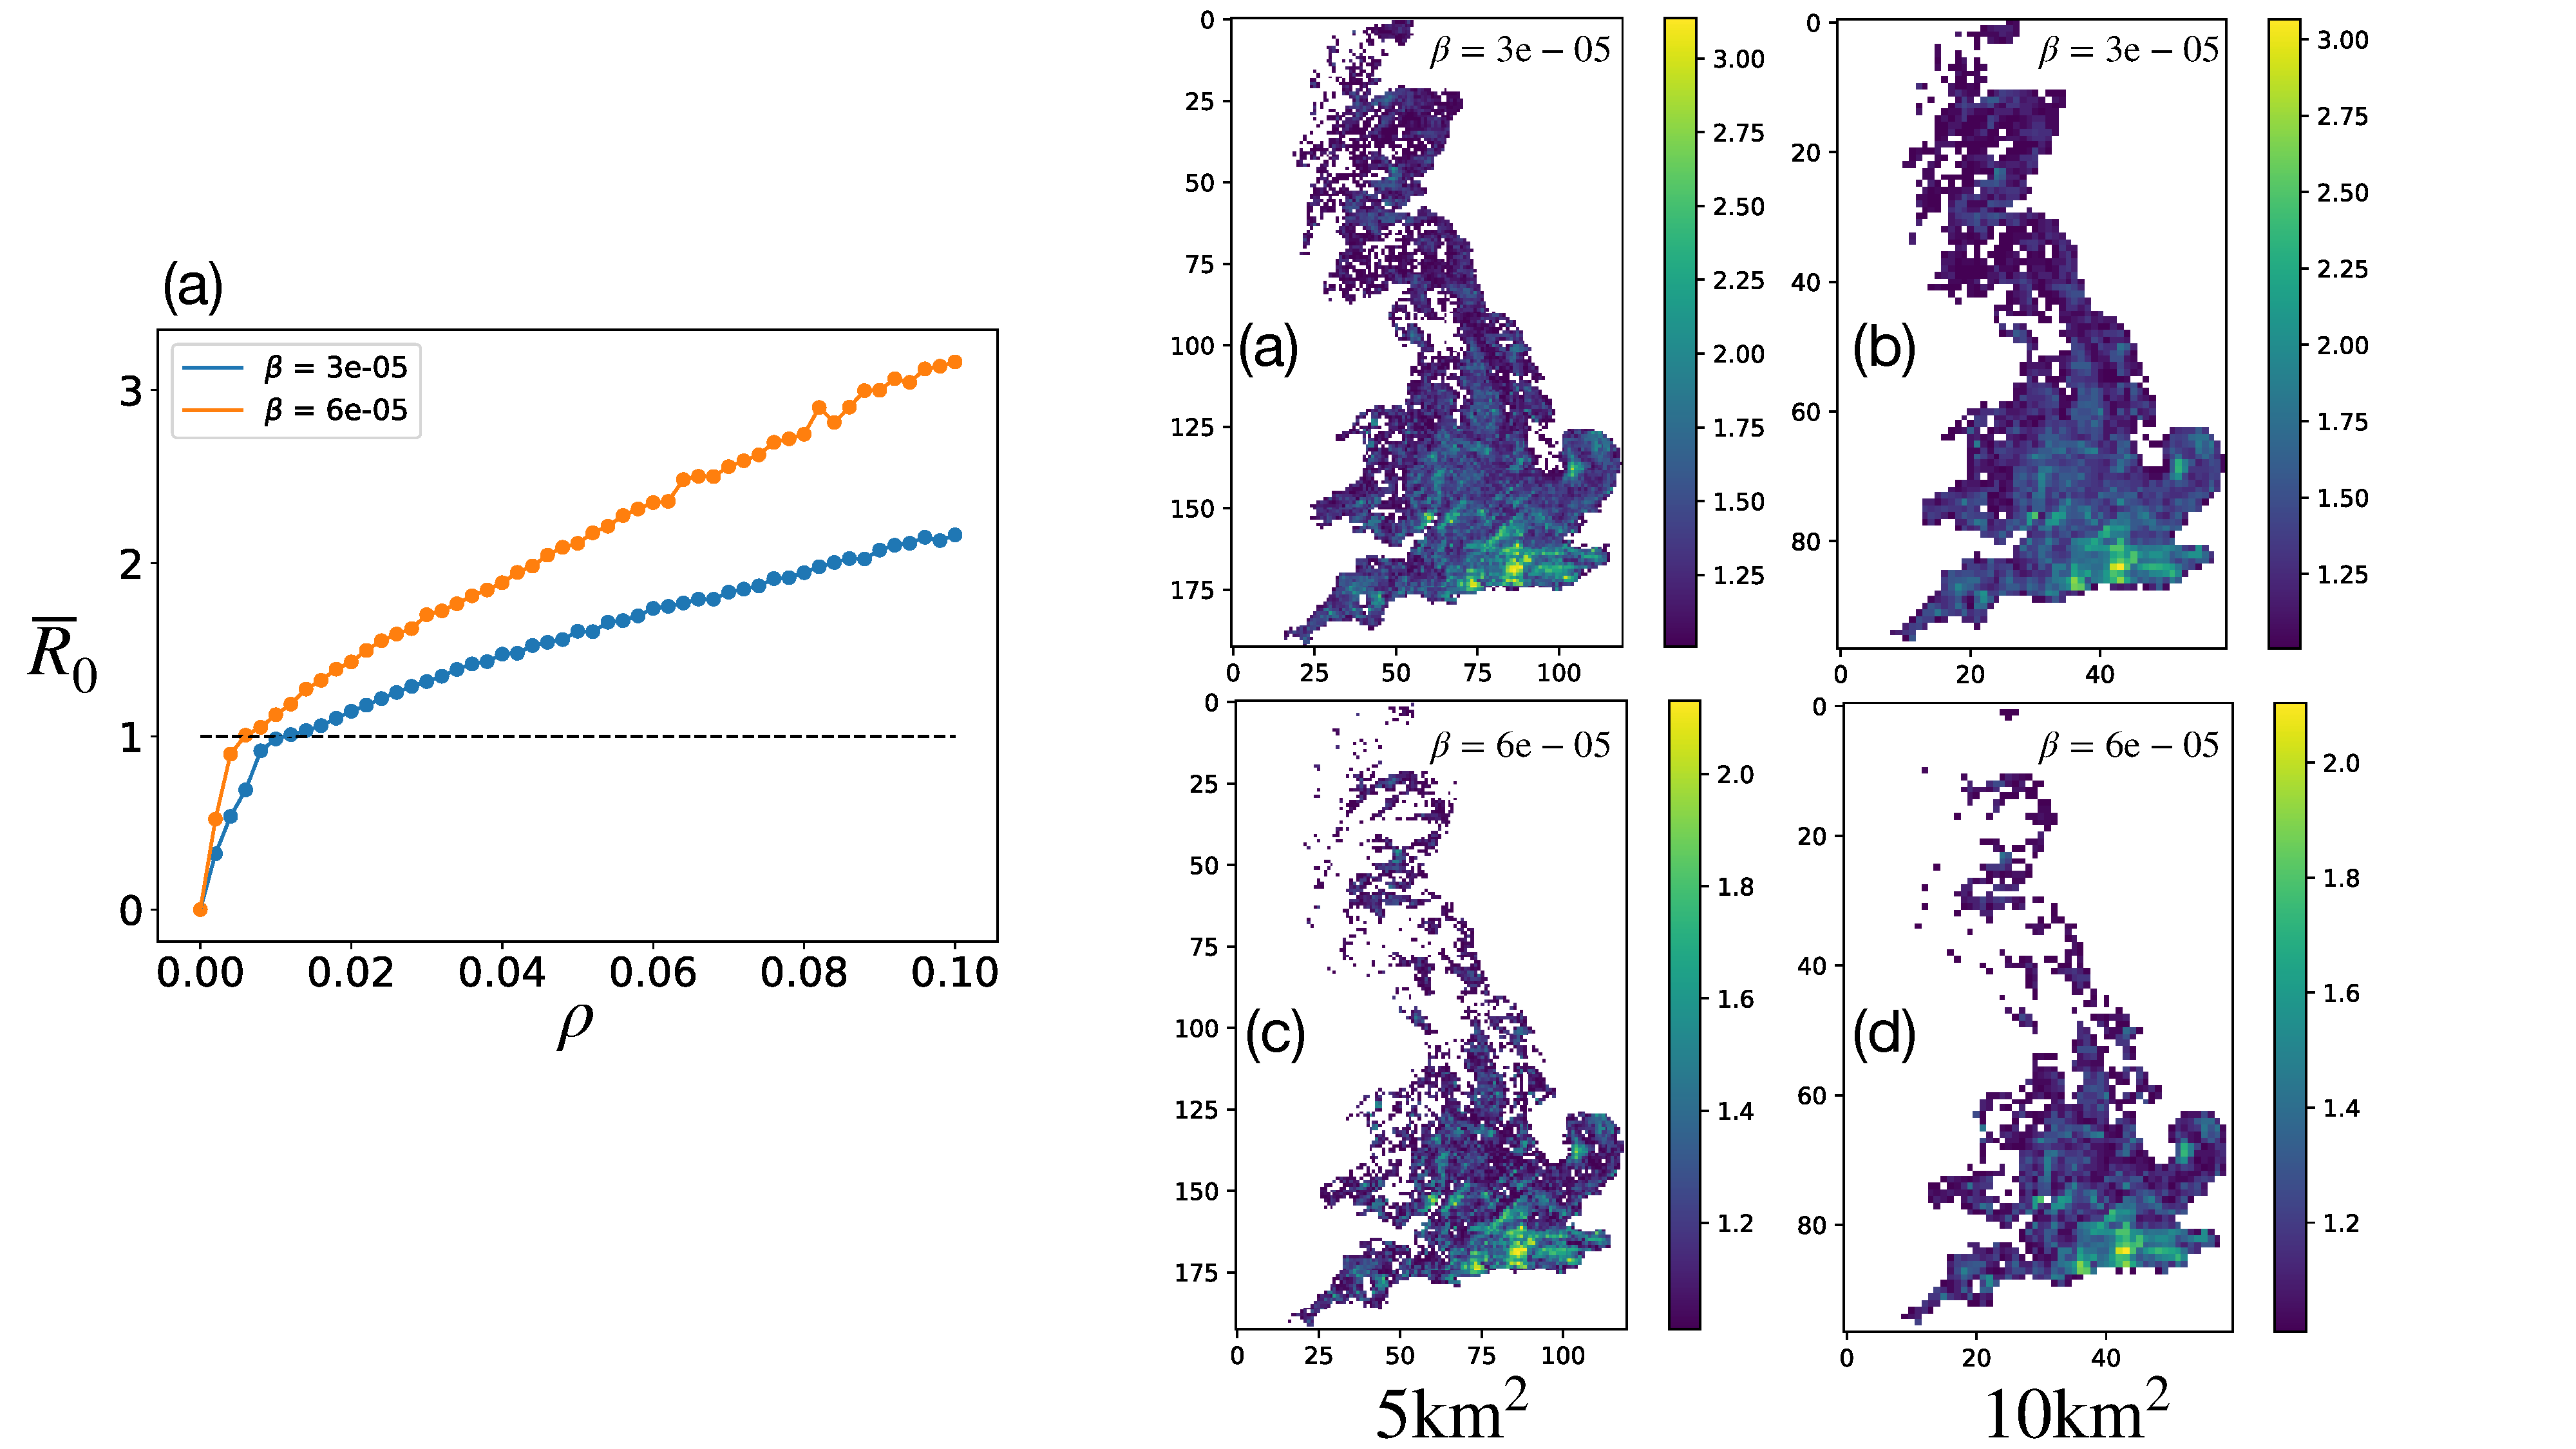
\includegraphics[scale=0.25]{chapter6/figures/fig2.pdf}
    \caption{Dispersal gradients at the local spatial scale, parameters are informed by the work of \cite{grosdidier2018tracking}. The authors provide estimates for Gaussian and inverse power-law kernels: $\ell_{ga} = 195\mathrm{m}$ and ($\ell_{pl} = 205\mathrm{m}$, $a=3.3$) respectively, where $a$ represents the inverse power-law exponent.}
    \label{fig:dispersal-parameterisation}
\end{figure}

Dispersal was informed by data collected in France by \cite{grosdidier2018tracking}. The field study conducted by \cite{grosdidier2018tracking} provide estimates for dispersal parameters by fitting data against a Gaussian and inverse power-law kernels. Notably, the authors studied dispersal at two different spatial scales, local and regional, \textcolor{red}{on the order of $1\mathrm{km}$, to $10-100 \mathrm{km}$ respectively}. For a review on the importance of scale, see chapter \ref{chapter2:litreview}. 

The experimental data analysed by \cite{grosdidier2018tracking} tracked ADB spores about known sources of infection. Although data on spore depositions does not necessarily correspond to a new infection, it sheds essential light on the spatial scale of ADB dispersal. Given that the spatial scale in the $SEIR$ model is small, at a  resolution of $5\mathrm{m} \times 5\mathrm{m}$, a decision was made to parameterise dispersal with the local-level dispersal values given by \cite{grosdidier2018tracking}. See table \ref{tab:SEIR-model} an Fig\ref{fig:dispersal-parameterisation}. 

The decision to use ADB scale parameters given by \cite{grosdidier2018tracking} suppose that the spread of ADB in Great Britain is comparative to the spread of ADB in France. Nonetheless, there is a noticeable difference in the French climate, landscape and, importantly, wind patterns. % references
Notwithstanding these differences, it stands to reason that dispersal parameters, if measured over a smaller, local spatial scale, would be less pronounced. 

Lastly, the regional-scale dispersal analysed by \cite{grosdidier2018tracking}, measured over spatial scales of $10$-$100\ \mathrm{km}$, is thought to contain artefacts of LDD by human-mediated transport. The regional spread of ADB though LDD is, therefore, beyond the scope of the present chapter\textemdash a discussion of LDD will conclude this chapter and lead us to chapter into chapter \ref{ch7:pde}.

% Q: what is the relationship between the mortality ratio (or final fraction of infected hosts) ? 
% If R0 was considered over a larger time-scale, host-regrowth would need to be integrated into the model
% Furthermore, measuring R0 over a larger time-scale could over, or underestimate, the degree to which a response would need to be undertaken in the response time-window. 
% a basic reproduction number $R_0$ is defined for the first life-cycle of the pathogen.
% Moreover, data over a relatively short time scale is typically all that is available when making decisions about control, not to mention the added complexity of incorporating host-regrowth–which becomes an important factor over longer time scales–and so, the constraint of computing R0 over longer time scales is relaxed. 
%  We develop the simplest implementation possible, namely, where R_0 is measured over one pathogen life-cycle, and the course of infection for each host follows the same process with perfect fidelity. This lies in stark contrast to a realistic scenario whereby different hosts show considerable differences.

% \begin{itemize}
%     \item see for a review on how R0 is calculated \cite{perspectives-on-r0}, we use method x in order to estimate and inform R0
%     \item $R_0$ is a complex function which changes in time, to this end, the next generation operator is used to derive a value for $R_0$ \cite{doi:10.1098/rsif.2009.0386}. In order to inform the value of $R_0$ we do xy and
%     \item Although it is hard to enforce a true $R_0$ value, the most important feature introduced from the definition is a threshold from which we can see if a local invasion is likely to take place.
%     \item Since the number of susceptible hosts is fixed, without replacement, the number of susceptible hosts will continually decrease in time in the case of an epidemic. Given the strong spatial component in the model we expect that measuring $R_0$ as-per this definition will give an under-estimate for later times when few susceptible trees remain. Likewise, for earlier times when susceptible neighbours are plentiful $R_0$ will yield an upper estimate for the pathogen. In order to characterise the pathogen in this model, we take the upper bound defined between the $1^{st}-2^{nd}$ generations. This simplification represents a worst-case scenario and the mean value of $R_0$ would be lower for later times when there are less trees available to infect. But most importantly, the threshold of transmission $R_0>1$ is reliable captured \textit{during the initial stage of infection}.
%     \item $R_0$ can be fully characterised by a growth rate \cite{R0-construct}. That is, the growth factor per generation.
% \end{itemize}

\section{Seasonal $SEIR$ model behaviour}

Previously in section \ref{sec:infection-dynamics} the details of sporulation were omitted. For robustness, two sporulation functions are considered, a step function defined by equation \ref{eq:step-function} and a normal distribution located at the midpoint between June and September. For now, the simplest form of sporulation is adopted:
\begin{equation}
\label{eq:step-function}
\phi(t) = 
\begin{array}{cc}
  \{ & 
    \begin{array}{cc}
      1 & t\in [\mathrm{June},\ \mathrm{September}] \\
      0 &  \mathrm{elsewhere}
    \end{array}
\end{array}
\end{equation}

The $SEIR$ model behaviour is shown in Figure \ref{fig:SEIR-spread} for the inverse power-law dispersal model over the average density of ash in Great Britain\textemdash see Appendix \ref{section:ga-SEIR-variant} for the Gaussian variant. During each season, a rise in the number of exposed trees in $E$ can be seen during summertime sporulation, June-September, followed by a rise in the number of infected trees in the Autumn, highlighted by Figure \ref{fig:SEIR-spread}(a). 

The spatial progression of ADB is shown in Figures \ref{fig:SEIR-spread}(b-d). The simulations begin from an initial condition of $25$ infected ash distributed throughout the host landscape. Each sporulation season leads to new secondary infections into the $E$ compartment, shown by the orange markers. The black markers depict a steady transition of infected ash into the $R$ compartment.

The number of ash in the $SEIR$ compartments over $10$ years is shown in Figure \ref{fig:SEIR-spread} for a domain of size $2\mathrm{km}\times2\mathrm{km}$ and three variations of the infectivity parameter $\beta$. Figure \ref{fig:SEIR-spread} shows three scenarios with infectivity parameters $\beta \in [2.5\times 10 ^{-4}, 1.5\times 10 ^{-4}, 1.5\times 10 ^{-5}]$, above, equal to and below the threshold for spread, (e-g) respectively.

Figure (g) highlights that even if the epidemic parameters are below the threshold, as indicated by the slow but steady decline of ash in $I$, the fungus may survive for long periods. This behaviour is known as `\textit{persistence}'. Persistence is, in general, one aspect of plant-based diseases that makes epidemic control difficult\textemdash see chapter \ref{ch3:invasions_and_persistence} for a review of invasion and persistence in the spread of plant-based diseases.  

\begin{landscape}
\begin{figure}
    \centering
    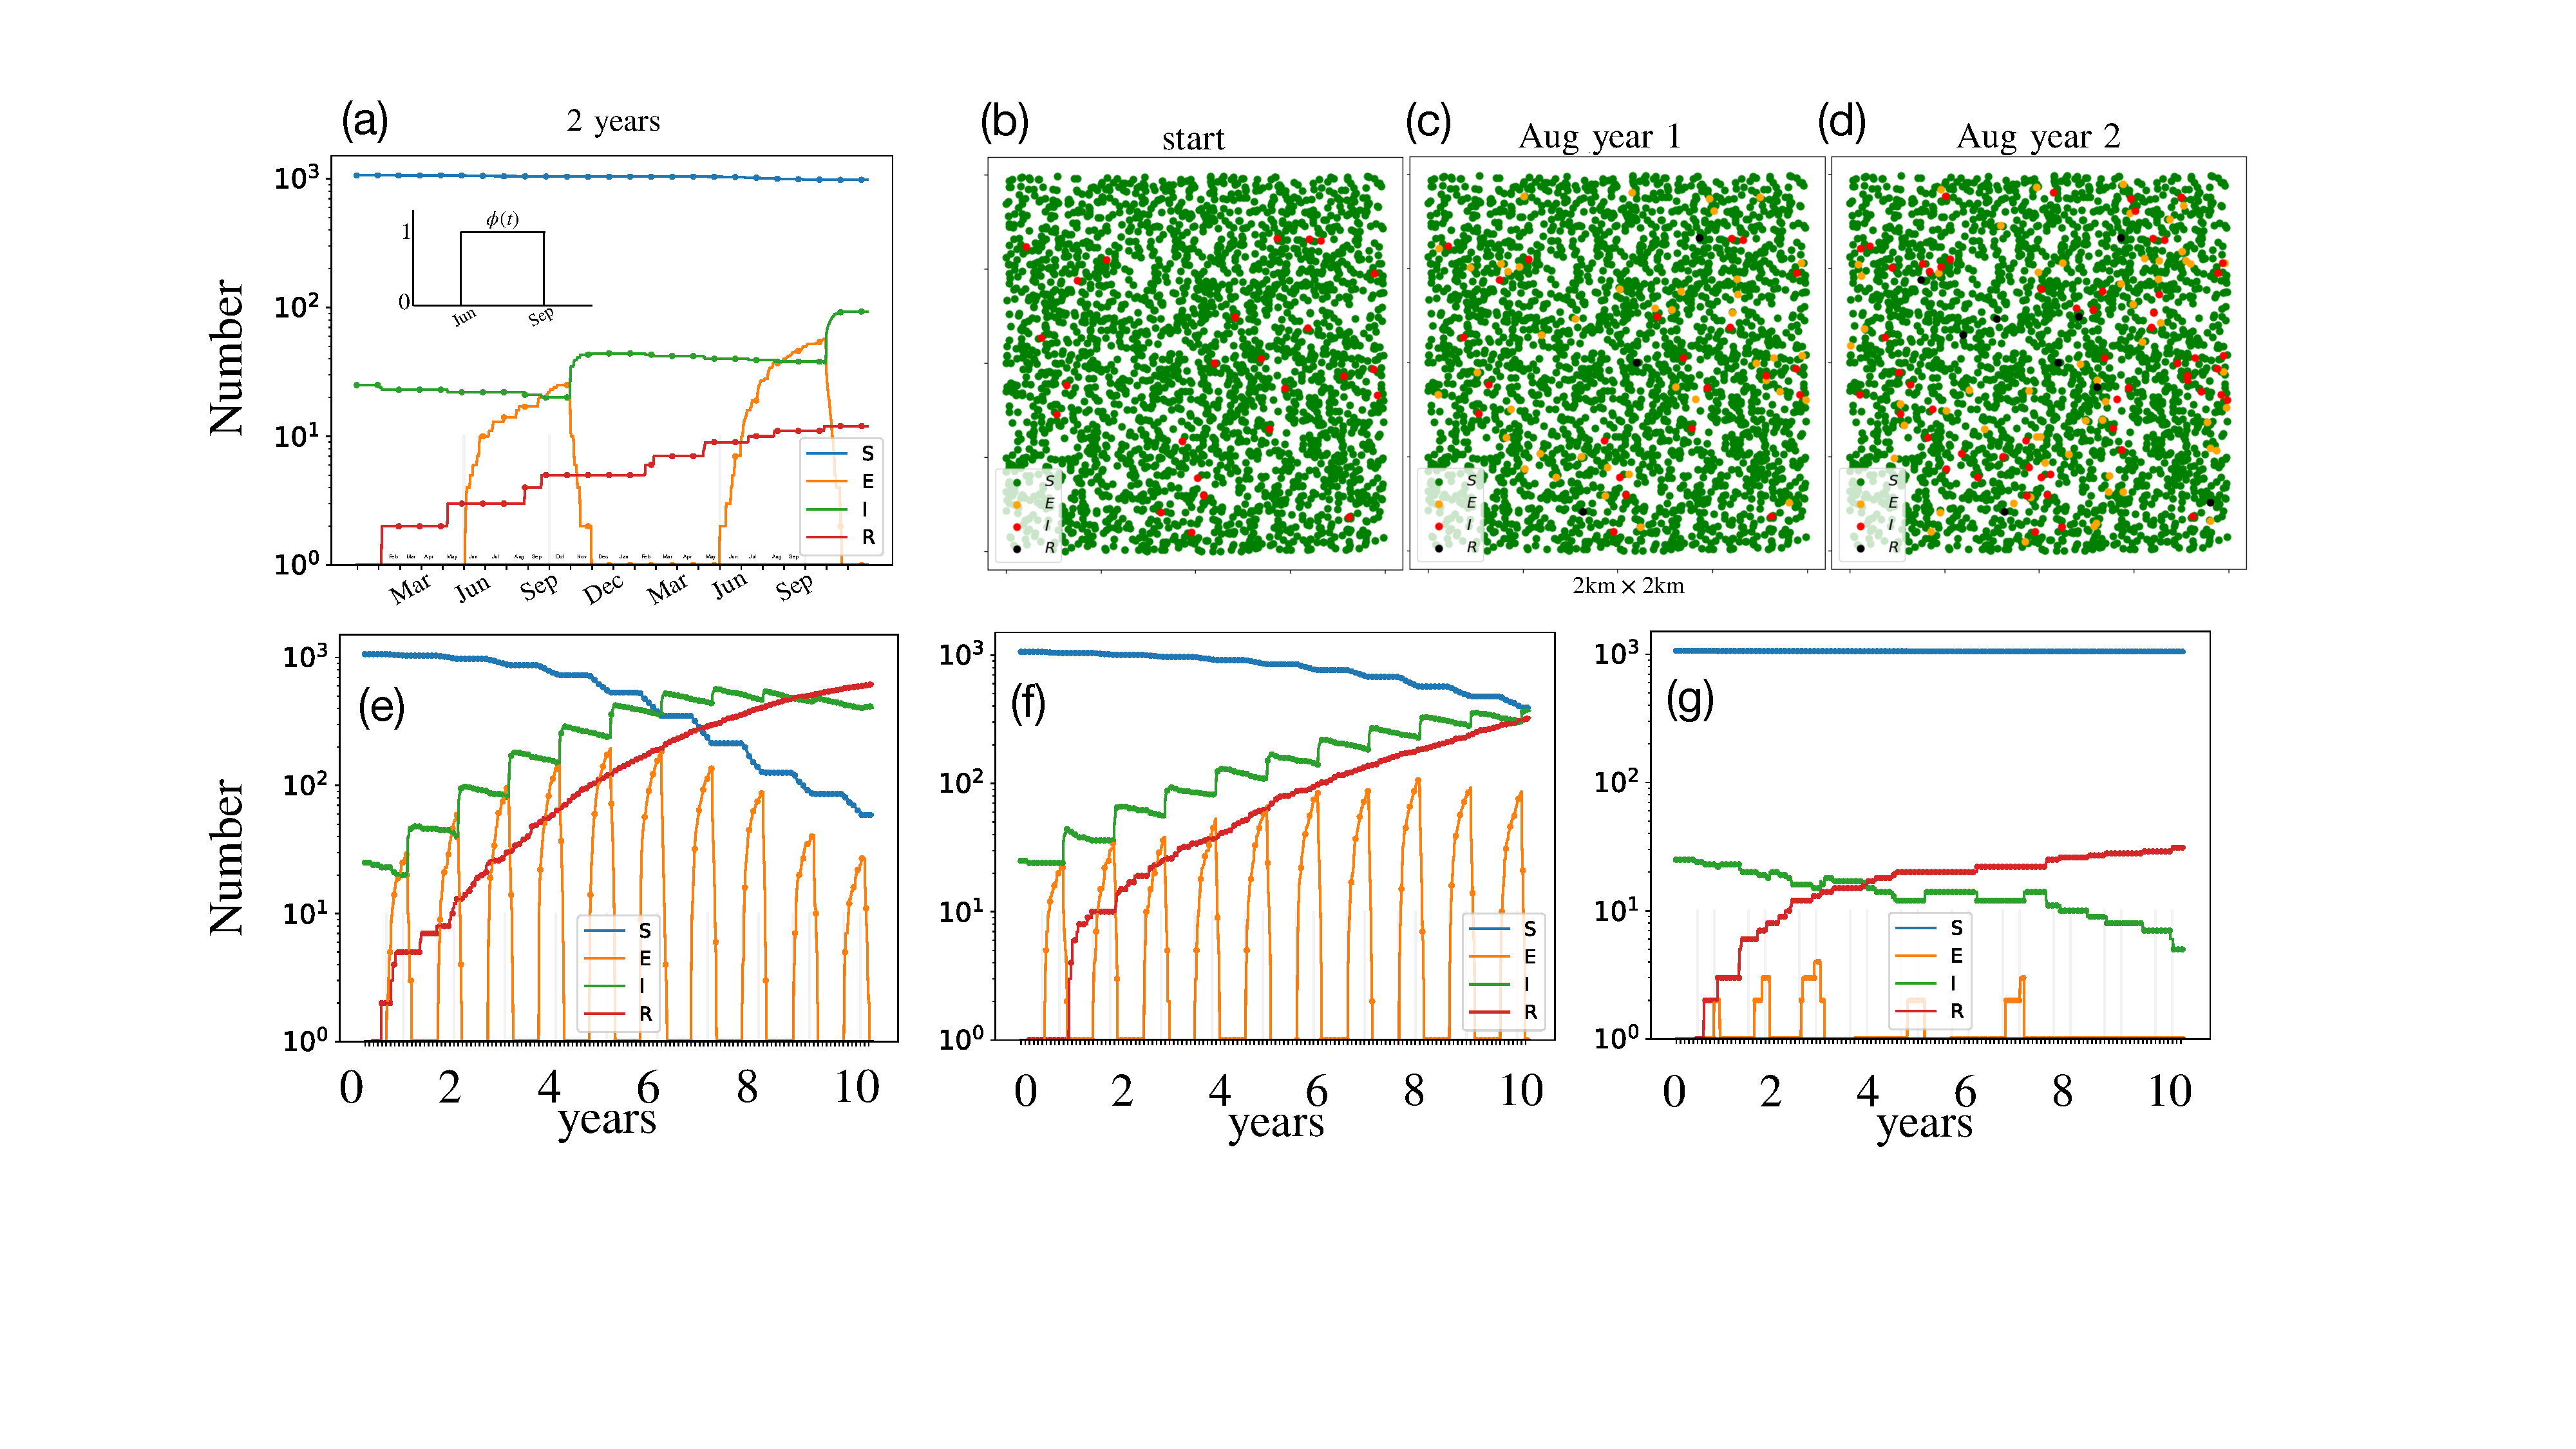
\includegraphics[scale=0.45]{chapter6/figures/fig4-seir.pdf}
    \caption{The number of trees in compartments $SEIR$ for the inverse power law model over the average ash density $\overline{\rho} = 0.017$. (a) A two year simulation above epidemic threshold, the inset axis shows sporulation function (b-d) The spatial progression of disease in a $2\mathrm{km} \times 2\mathrm{km}$ domain.(e-g) Simulations show the epidemic progression over ten years above, around and below the threshold.}
    \label{fig:SEIR-spread}
\end{figure}
\end{landscape}

\subsection{Sporulation}
\textcolor{red}{demonstrate a Gaussian-based sporualation function...}

\section{Defining an $R_0$}

\begin{figure}
    \centering
    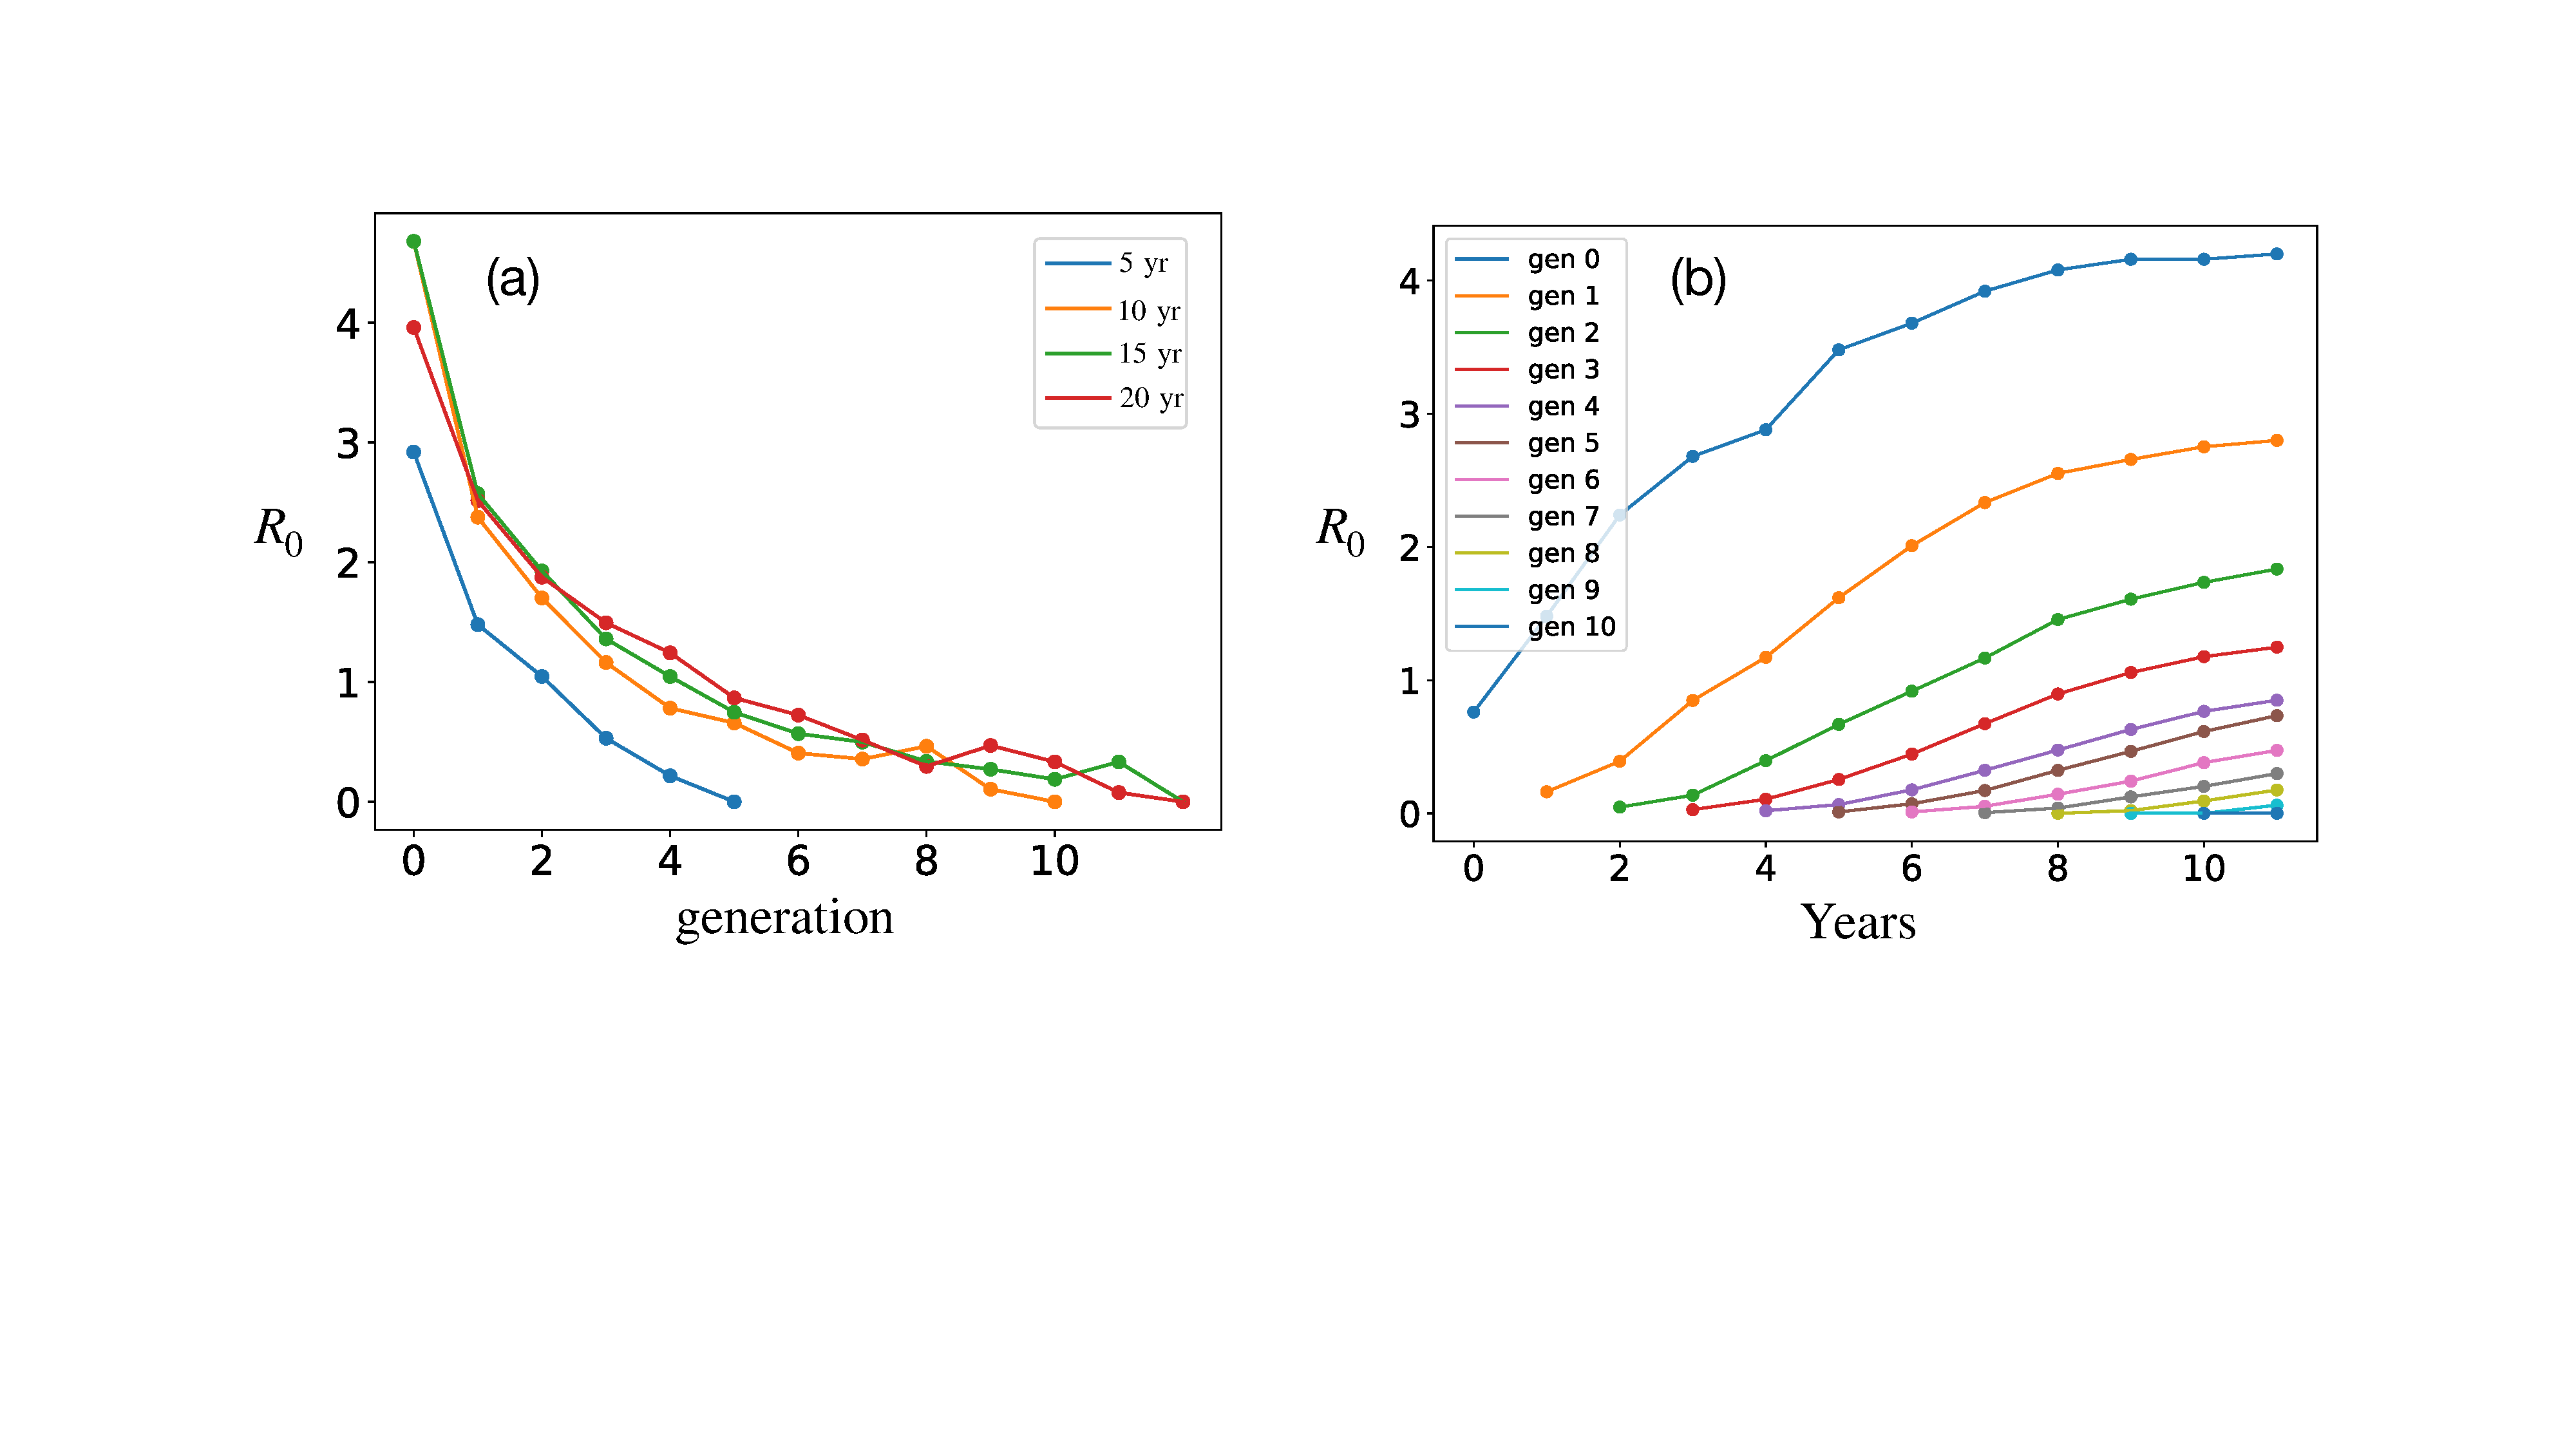
\includegraphics[scale=0.3]{chapter6/figures/fig5-R0-def.pdf}
    \caption{Contact-tracing $R_0$ in the seasonal $SEIR$ model. (a) The average number of secondary infections are shown for ash infected in the $n^{th}$ generation after outbreak (b) The average number of secondary infections is shown against the years after outbreak for different generations $0-10$.}
    \label{fig:SEIR-R0-definition}
\end{figure}

Before the $SEIR$ model can be investigated, a measure of the pathogens ability to invade must be defined. For epidemic systems, this usually comes in the form of a reproduction number $R_0$. There are, however, various challenges involved in defining $R_0$ when there are dispersal-mediated secondary infections and spatial structure, as explored in chapter \ref{ch5:dispersal-model}. Chapter \ref{ch5:dispersal-model} demonstrated that $R_0$ is a spatiotemporal function of various epidemiological parameters, and measuring $R_0$ over different spatiotemporal scales can lead to different, and sometimes misleading, results for $R_0$; for a seasonal-based pathogen such as ADB, additional factors only complicate the definition. 

\textit{From this point on, unless otherwise sated, the method for calculating $R_0$ will refer to the average number contact traced secondary infections for each generation of infection, as per Definition \ref{def:R0_contact_traced}. However, this time, secondary infections characterise the transition $S\rightarrow E$ and successive generations of infected ash arise seasonally during sporulation.}

As demonstrated in chapter \ref{ch5:dispersal-model}, a suitable spatial and temporal scale must be chosen to measure $R_0$. Figure \ref{fig:SEIR-R0-definition} shows the contact-traced $R_0$ for the power-law model $SEIR$ spreading above the threshold\footnote{The Gaussian variant of the $SEIR$ model also follows the same characteristic decline in $R_0$ for each subsequent generation, as demonstrated in chapter \ref{ch5:dispersal-model}}. For the particular combination of pathogen parameters shown in Figure \ref{fig:SEIR-R0-definition}(a), $R_0$ saturates to around $4$ and there is little difference in measuring $R_0$ between $10, 15$ and $20$ years. Although, measuring $R_0$ over a five year is slightly below the $10-20$ year average. This behaviour is also reflected in Figure \ref{fig:SEIR-R0-definition}(b) where $R_0$ for the first generation infected ash saturates at around $R_0 = 4$. On average, we would expect to see more infectious pathogens saturate faster and less infectious pathogens take longer\textemdash see Appendix \ref{fig:a-R0-saturate}.

From Figure \ref{fig:SEIR-R0-definitio}(a-b) we can see the familiar saturation of $R_0$ for later generations. The decline in $R_0$ with each generation can be understood by the decline in susceptible ash with time. The first generation infected ash, at $t=0$, have a higher number of susceptible neighbours available to infect, which declines in time. The saturation point of $R_0$ mirrors the infectious lifetime which, in this model are taken to be exponentially-distributed with mean $\lambda=5\ \mathrm{yr}$. In light of better data, this choice of distribution and parameterisation could be updated. 

It makes sense to define a measure for $R_0$ based on the first generation of infections, given that the first generation has, on average, a higher $R_0$. Choosing an $R_0$ in this manner gives us an upper-bound of invasiveness, which for control, is better than an under-estimate:

\textit{The results of this, and the proceeding chapter, therefore, are based on the average number of first generation infected ash.}

Lastly, a suitable domain size $5\mathrm{km} \times 5\mathrm{km}$ was chosen to measure the $R_0$ for first generation infected ash over a $10$ year period. Primarily, this choice was taken for two reasons: 1) larger domain sizes beyond $5\mathrm{km} \times 5\mathrm{km}$ incur increasingly larger computer run times 2) there is little dependence of $R_0$ at, or beyond, this domain size or most values of $\beta$. Although, as shown in Appendix \ref{a:seir-with-L}, it is possible to under-estimated $R_0$ for high values of $\beta$, albeit slightly.


% - Show three different values of beta, above below and at threshold, for ga vs pl 

%\subsection{Defining an R0 value}
% Show that R0 A) over the season B) the problem policy makers experience by not having 5 years to wait before estimates of R0 C) How to form a crude estimate for R0 based on the first season 

% \subsection{Towards $\beta$ parameter-matching}
% - using mortality/infection \% data over match beta against percentage infected

% \subsection{Persistence}
%  - use a 10 year simulation below seasonal threshold, to show that the pathogen can survive for long periods within an area


% discuss multiple sporulation functions

% A simple time-dependant function $\phi(T)$ takes the value of $1$ between the summer months of June - September, and $0$ otherwise thus reflecting the sporulation peak of \textit{Hymenoscyphus fraxineus} (HF). During these summer months, wind-borne dispersal occurs when fruiting bodies produce large numbers of ascospores. 

\section{Informed ash density maps}

Up to this point, a thorough description of the host data set has been omitted. Ash densities are parameterised by modelled ash abundance data provided by \cite{hill.data}. The canopy cover datasets produced by \cite{hill.data} combine a number of different data sources that cover parts of Great Britain, regression methods are then used to extrapolate canopy cover over the whole of Great Britain\footnote{Previously in chapter chapter \ref{fig:ch4_uk_spread}, the oak canopy cover dataset given by \cite{hill.data} was used in conjunction with the SLM toy model; the insights from doing this then motivated the construction of a generic $SIR$-based dispersal model in chapter \ref{ch5:dispersal-model}.}. Conveniently for the present chapter, ash happened to be among the most accurate data sets given by \cite{hill.data}. For a more in-depth description of the methods used by \cite{hill.data} and a review of host data in general, see chapter \ref{chapter:lit-rev}.

\begin{figure}
    \centering
    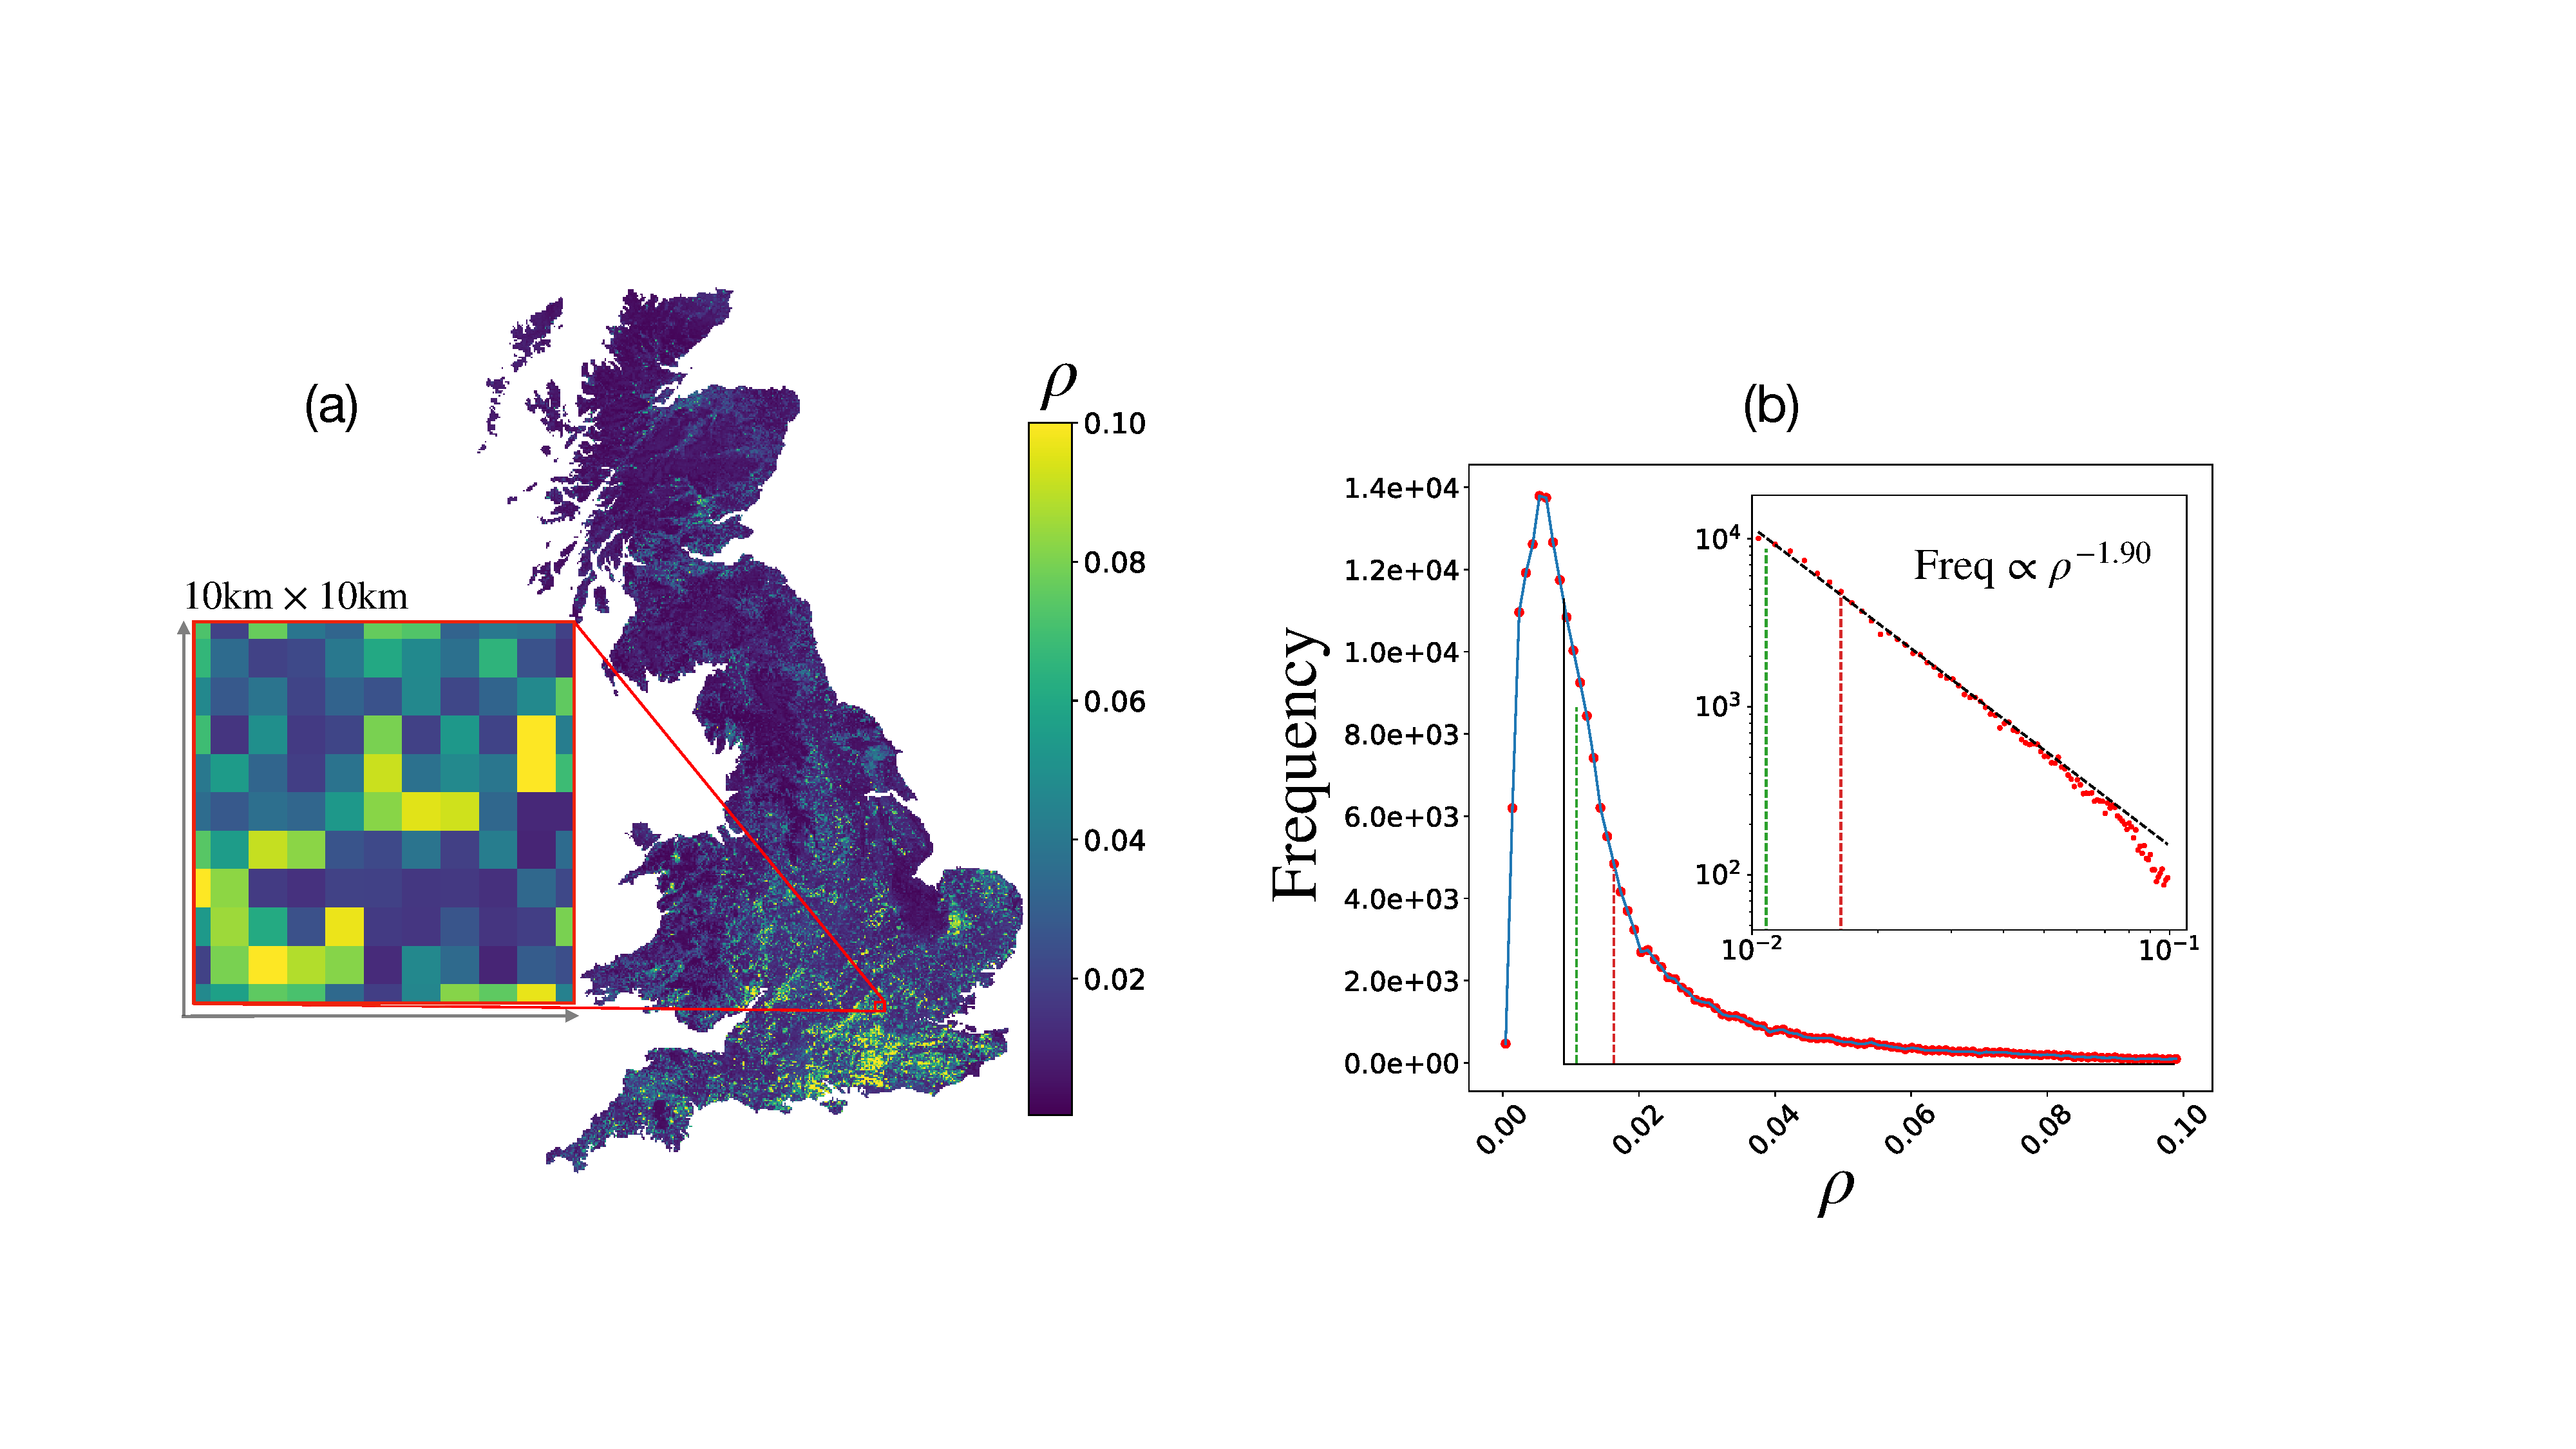
\includegraphics[scale=0.30]{chapter6/figures/fig3-ash-data.pdf}
    \caption{Ash canopy cover data, as modelled by \cite{hill.data} converted into a density. (a) a map of ash densities at a resolution of $1\mathrm{km} \times 1\mathrm{km}$ (b) the distribution of ash density over Great Britain, the inset shows a power-law behaviour.}
    \label{fig:ash-host-data}
\end{figure}

Figure \ref{fig:ash-host-data}(a) shows a density map of ash, at a resolution of $\mathrm{1km}\times \mathrm{1km}$, produced from abundance data given by \cite{hill.data}. From Figure \ref{fig:ash-host-data}(a), the south of England contains the highest concentration of high-density ash patches and ash become progressively less abundant in Scotland and coastal locations, in western Whales for example. A higher density of ash can be expected to yield a higher number of secondary infections, in line with the results of chapters \ref{ch3:two-param-model}-\ref{ch5:dispersal-model}.
 
 The frequency distribution is shown in Figure \ref{fig:ash-host-data}(b) and reveals that the average density of ash in Great Britain is $\rho=0.017$ and that few locations support densities of $\rho=0.10$ and over\footnote{In the original $2.2\times 10^4$ $1\mathrm{km^2}$ data points, there were a handful of outlier points with densities in the interval $\rho \in [0.10, 0.30]$ which were excluded from the analysis.}. Between the limits of $\rho \in [10^{-2}, 10^{-1}]$, the frequency distribution in Figure \ref{fig:ash-host-data}(b) follows a power law of the form $\sim \rho ^{-k}$, as evident from the linearity on the logarithmic inset axes. The distribution had a fitted exponent of $k=1.90$, shown by the dashed black line. Intriguingly, this observation is suggestive of self-similarity in the data.

Two modifications had to be made to the modelled ash canopy cover data in order to complement the $SEIR$ model. Firstly, the raw abundance values were re-scaled into a dimensionless tree density $\rho$. The same process was outlined in chapter \ref{ch5:dispersal-model} i.e. by converting the units $\mathrm{ha/km^2}$ to kilometre-squared of ash cover per kilometre-squared of land. Secondly, the map resolution has to be re-scaled to reflect the intrinsic spatial scale of local wind-borne dispersal, this topic is resumed below in section \ref{ch6:re-scaling-host-data}, when ADB $R_0$-maps are constructed over Great Britain.

\section{Constructing $R_0$-maps over Great Britain}

The invasiveness of a pathogen is though to vary over a landscape \textcolor{red}{citations}. A map of $R_0$ values would therefore be useful to policy makers and plant modelers alike. In this section we will project a set of $R_0$ values over Great Britain for the $SEIR$ model of ADB. Doing so will permit the investigation of a control strategy. 

\subsection{Tree density and $R_0$}
\blindtext

\subsection{Re-scaling the host distribution}
\label{ch6:re-scaling-host-data}

Suppose there are three patches of land, two that have tree densities above the threshold $R_0 = 1$ which are separated by an intermediary patch below the threshold. If we are not careful, it would be possible for pathogen dispersal to traverse the below-threshold patch of land within a single jump even at local spatial scales. As such, it is important we choose a domain resolution that gives some level of assurance that at the local scale, wind-dispersed spores cannot jump over whole patches with singular jumps. There is always the possibility that spores travel larger distances, from mainland Europe to Great Britain, for example, \cite{freer2017tree, wylder2018evidence}. Nevertheless, this chapter is predicated on targeting dispersal at local scales, and LDD can be omitted for now.

In the local scale field study conducted by \cite{grosdidier2018tracking}, fungal spores were only detected at a maximum distance of $500\mathrm{m}$ away from a known source of infection. So on the surface, the original $1\mathrm{km} \times 1 \mathrm{km}$ resolution of the abundance data, as reported by \cite{hill.data}, appears reasonable. However, with moderate-high values of $\beta$ the power-law $SEIR$ model demonstrates that singular jumps can exceed $1\mathrm{km}$ and since we cannot know $\beta$ for sure, it is desirable to air on the side of caution and re-scale the domain.


\begin{figure}
    \centering
    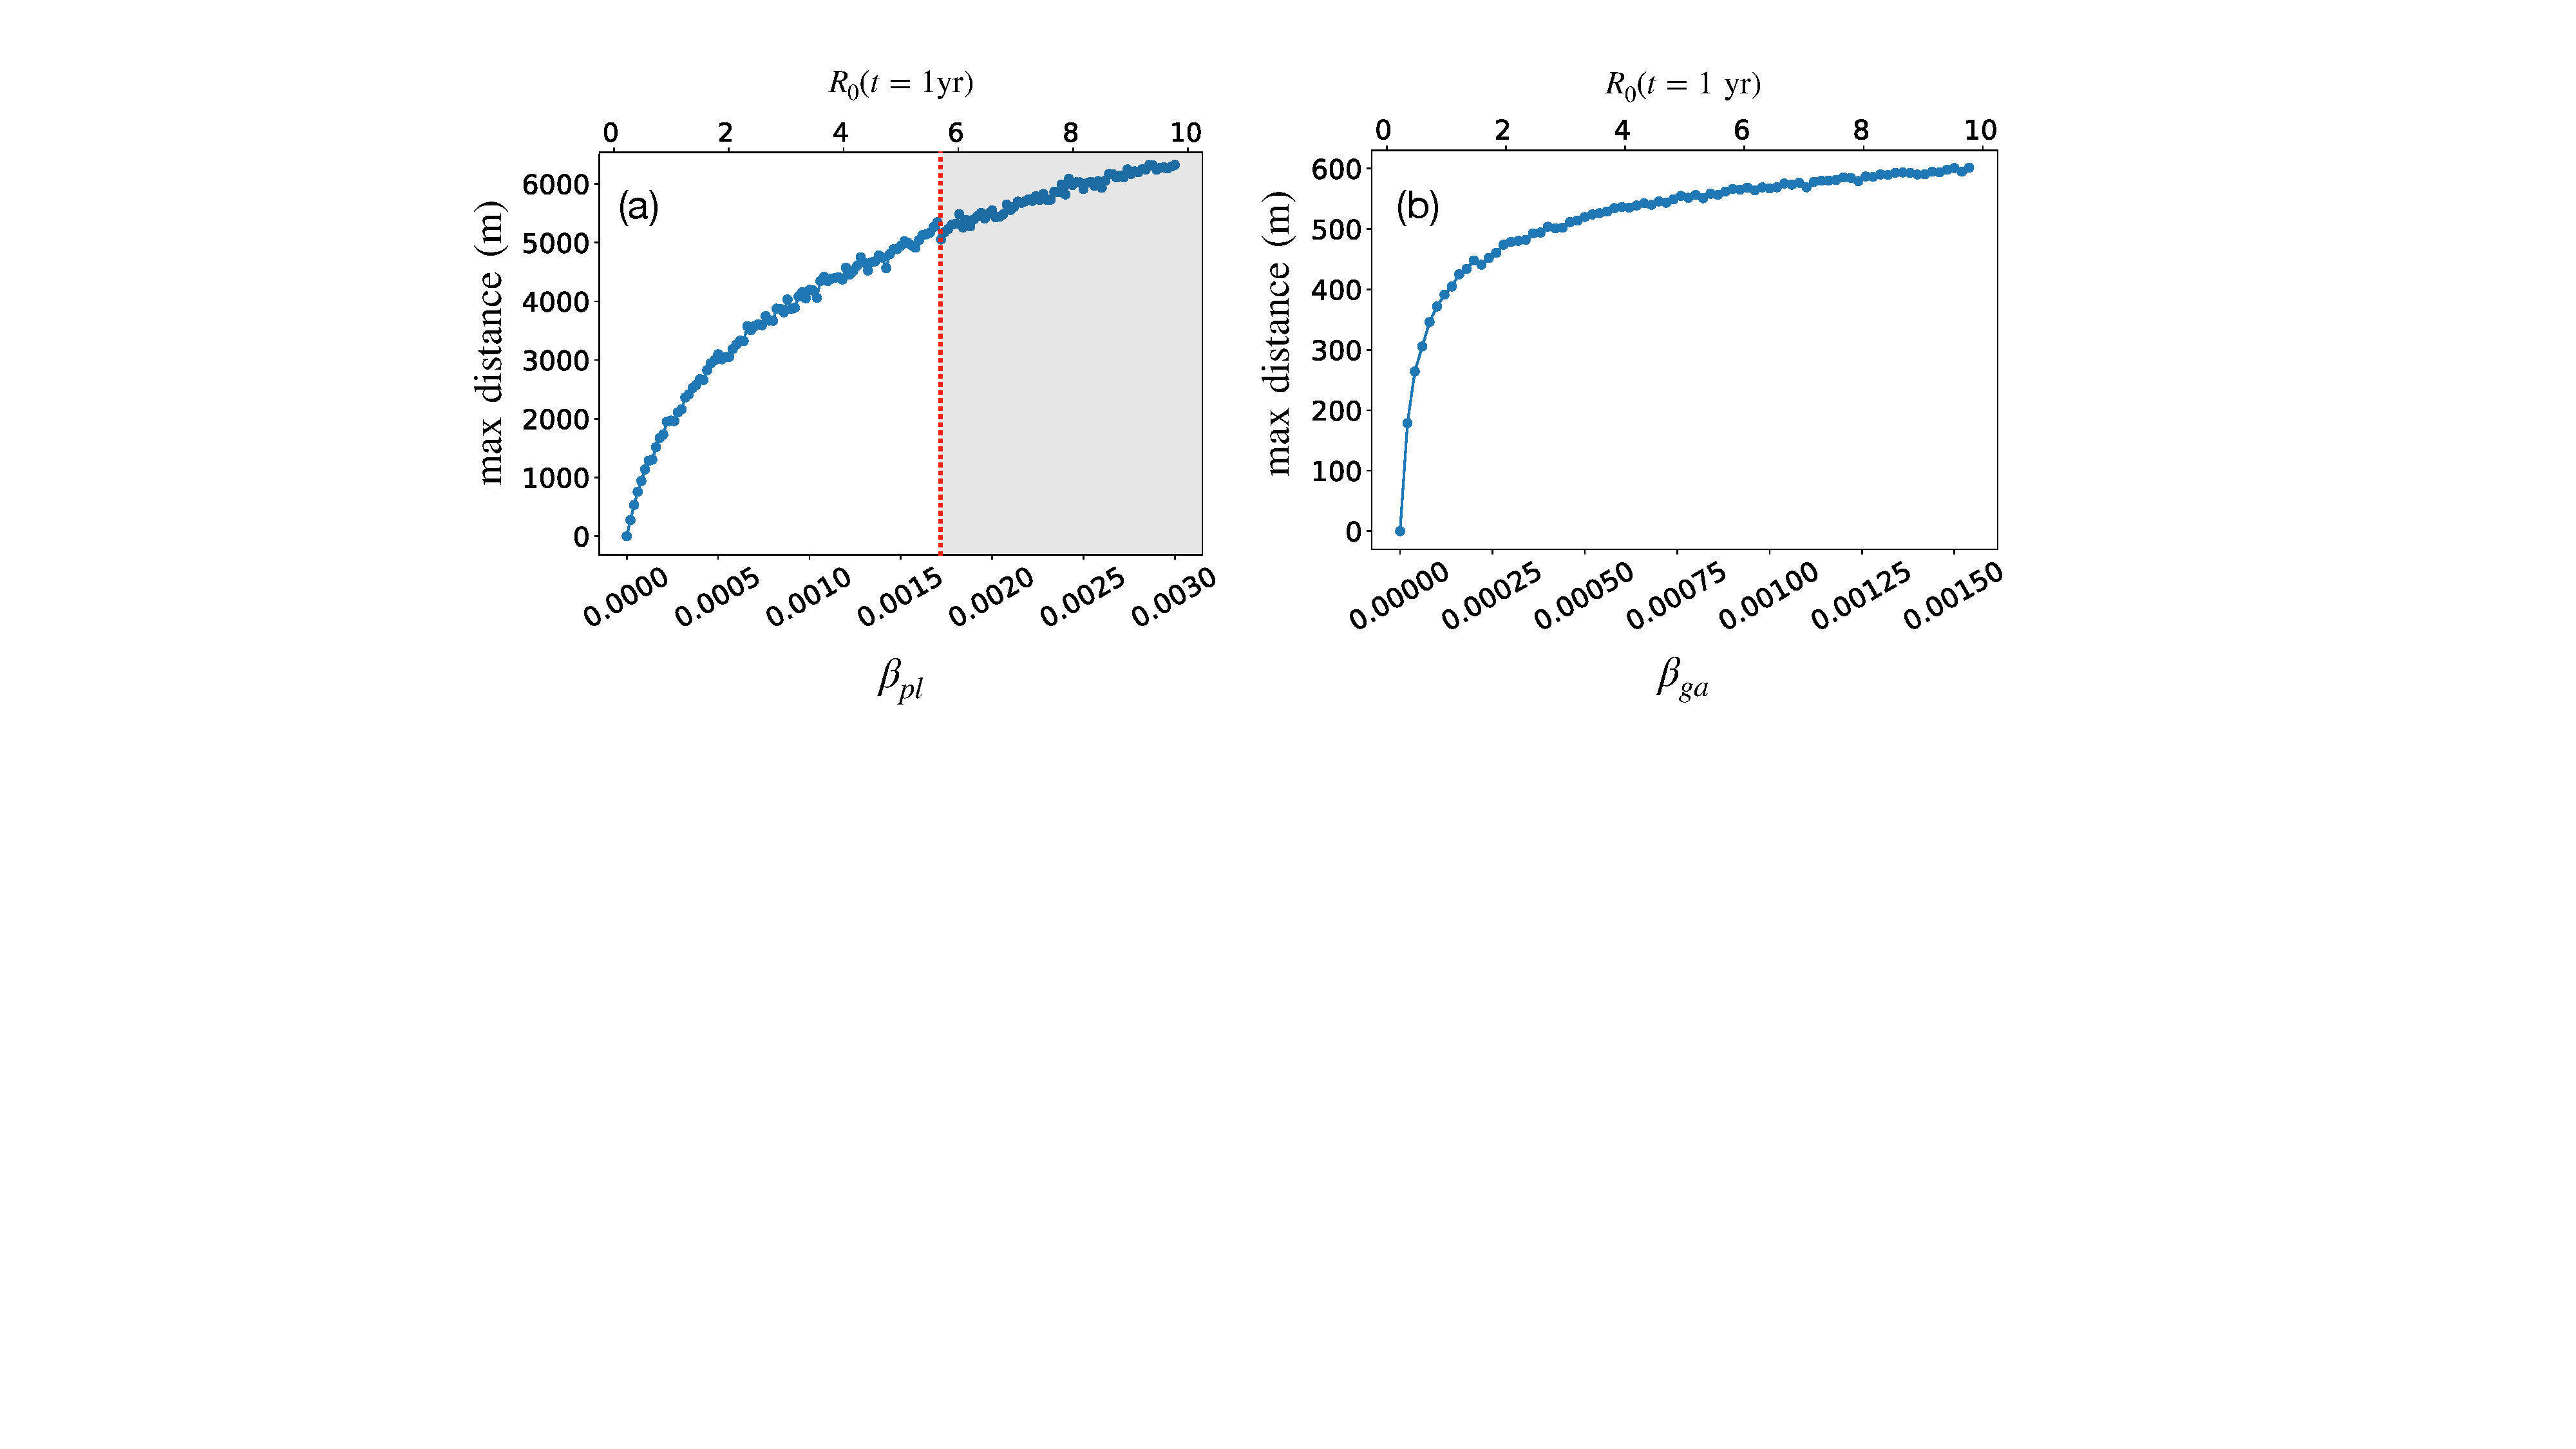
\includegraphics[scale=0.40]{chapter6/figures/fig5-beta-vs-max_d.pdf}
    \caption{Caption}
    \label{fig:my_label}
\end{figure}

% \begin{figure}
%     \centering
%     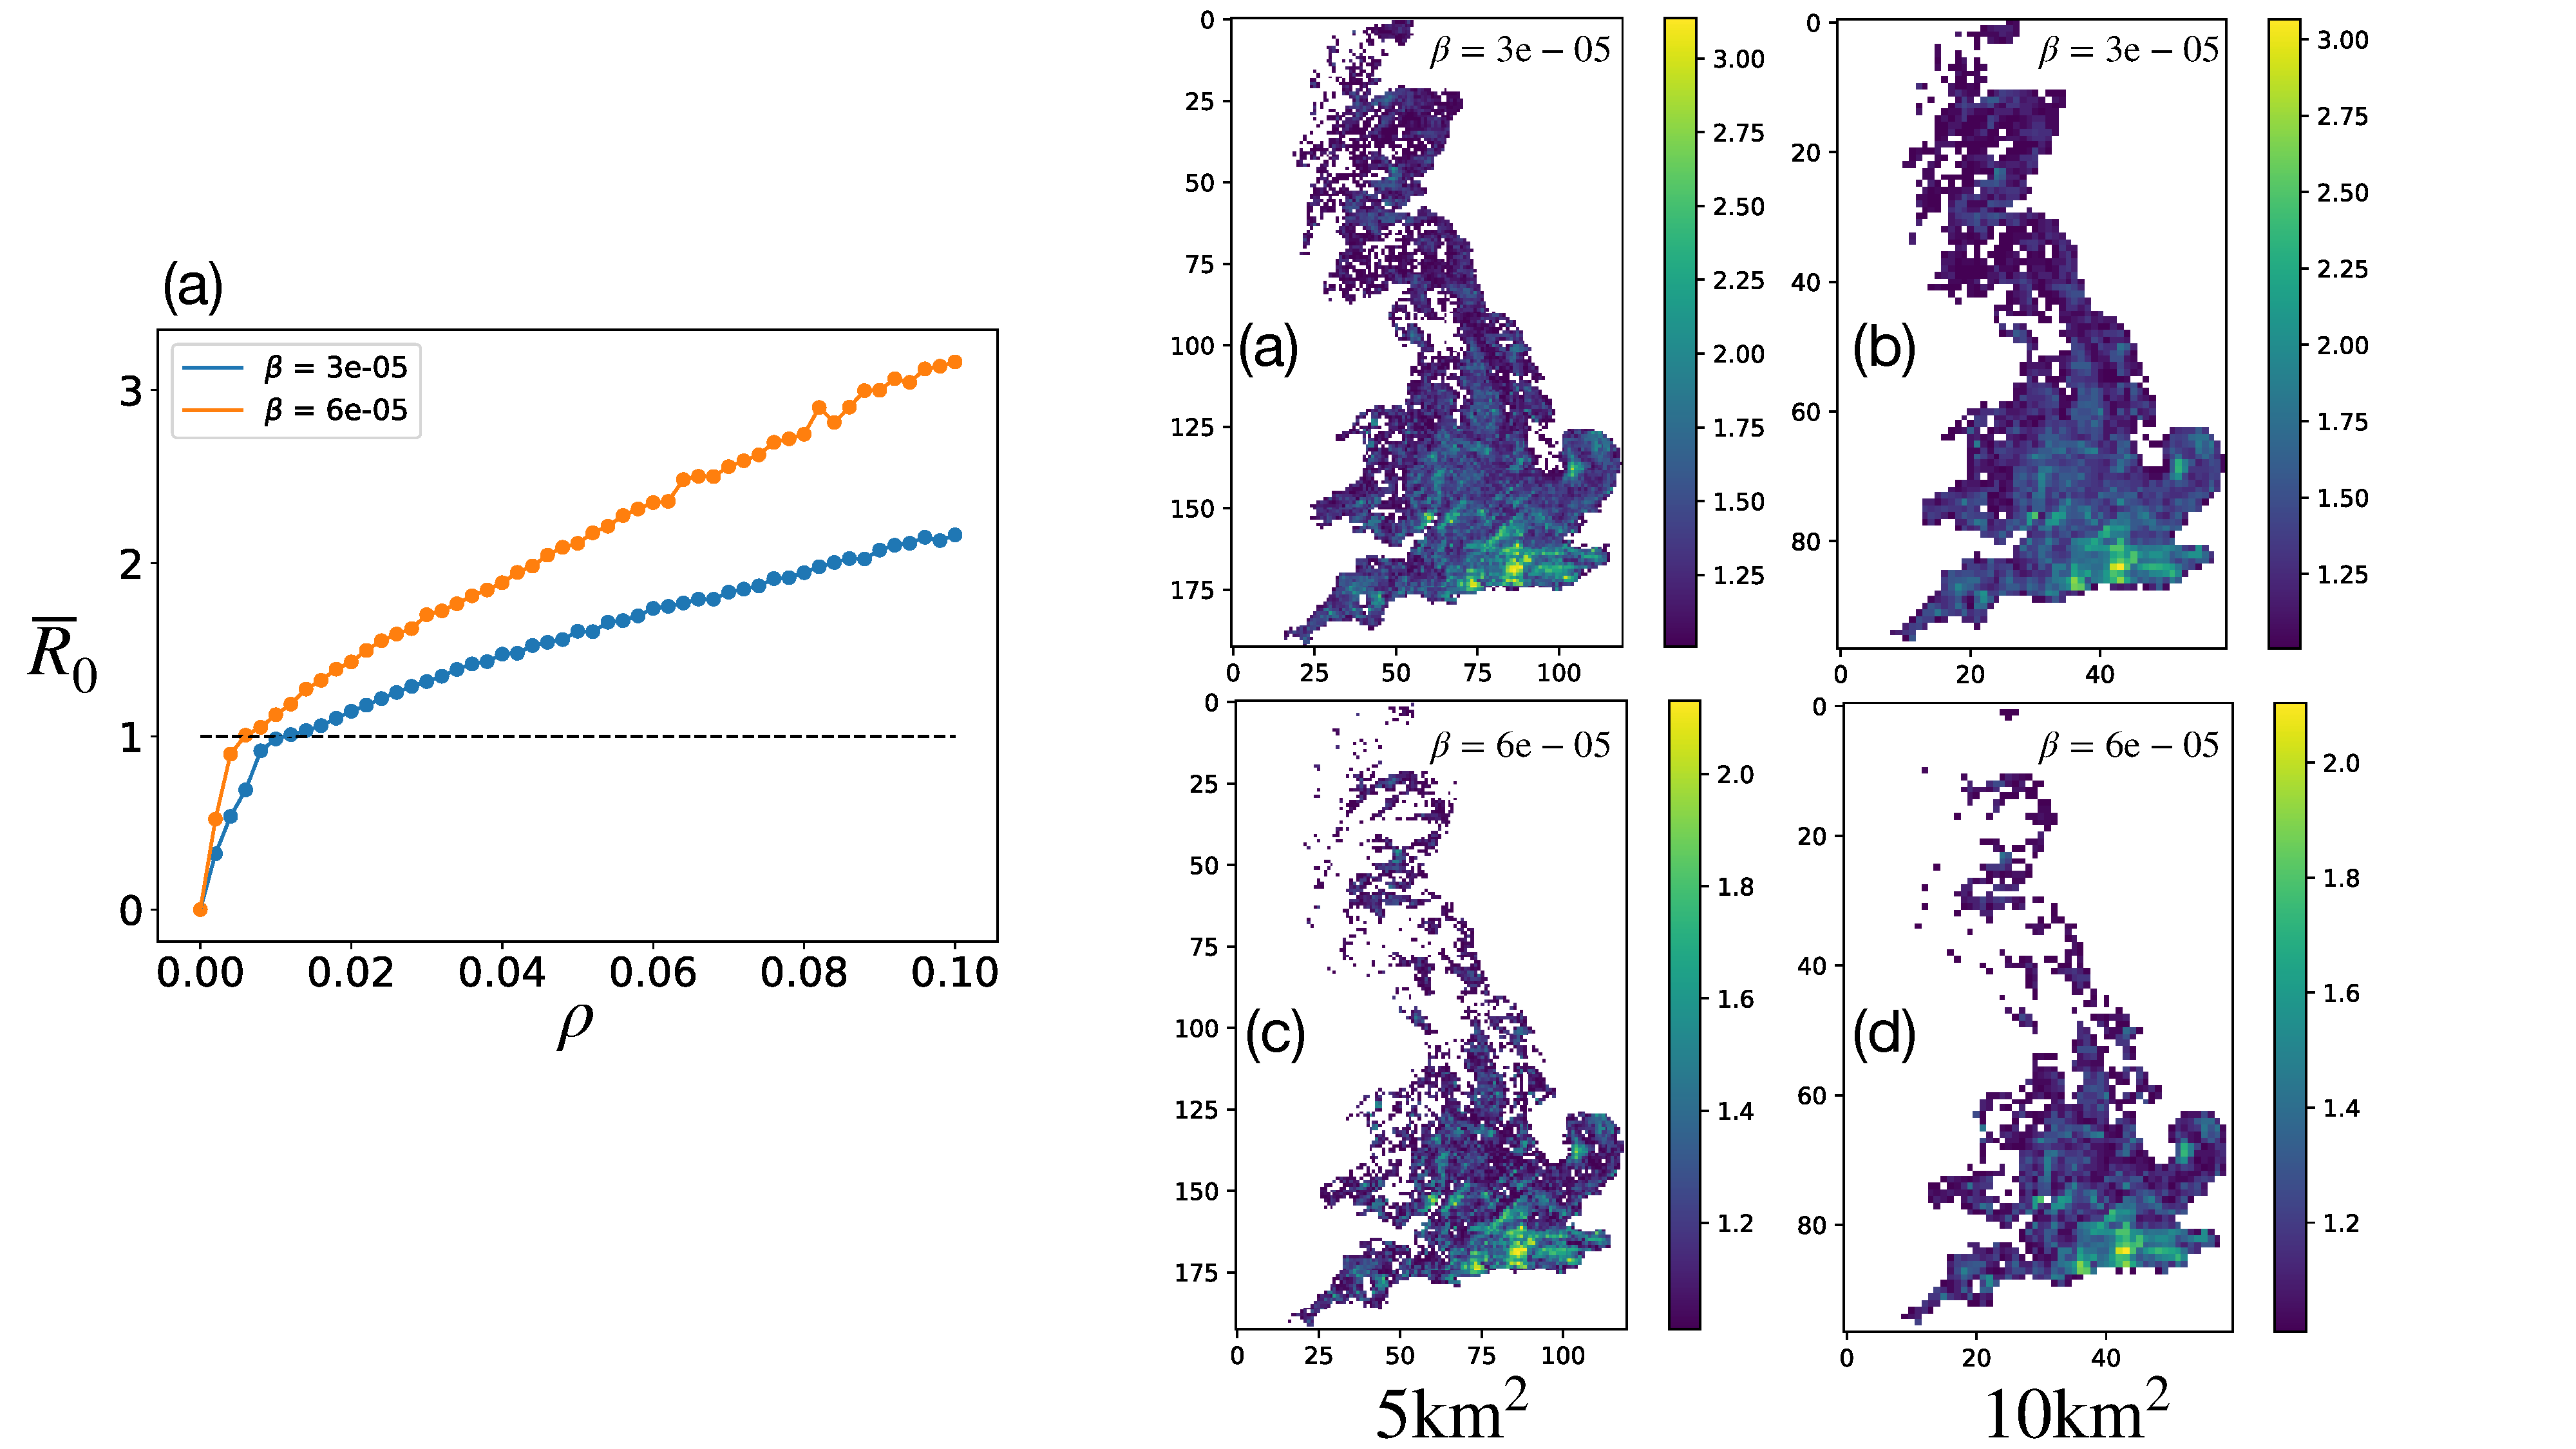
\includegraphics[scale=0.25]{chapter6/figures/fig4.pdf}
%       \caption{(a) Ensemble-averaged $R_0$ between two values of $\beta$, for Gaussian dispersal of $\ell=1.6\mathrm{km}$. (a-b) $R_0$-map for $\beta=3\mathrm{e}-05$, coarse-grained at $5$, $ 10\mathrm{km^2}$. (c-d) $R_0$-map for $\beta=6\mathrm{e}-05$.}
%     \label{fig:uk-mapping}
% \end{figure}


% 1 ) Show R0 vs beta vs max d 2) take betas < 5km 3) explain that if beta is larger, we need a bigger re-scaling.


% \footnote{A review on the landscape epidemiology of ADB \cite{doi:10.1111/1365-2745.13383} concluded that the effect of host abundance in the neighborhood of ADB decayed with distance, according to an exponential distribution with scale parameter $200\mathrm{m}$. That is, the severity of ADB symptoms depended on the surrounding abundance of ash.} 
% 

% discuss  projecting R0-maps
% Assumption, there is considerable genetic variation in susceptibility that varies between spatial location \cite{stocks2017first}

% In Figure\ref{fig:uk-mapping}, we can begin to identify heterogeneity and high-risk clusters of Ash. However, visualising which pixels connect to form large clusters is non-trivial. An image processing technique, `connected component analysis' (or CCA) \cite{CCA1, CCA2}, was used to identify and label susceptible clusters and simplify the $R_0$-map. This was performed using the function `label' from the Python-SciPy package `ndimage' \cite{scipy}. Doing so classified all susceptible (Moore) neighbours as connected members of the same cluster. \textcolor{red}{Figure \ref{fig:uk-mapping}(b) shows the top 10 largest $R_0$-clusters found in the map of Figure\ref{fig:uk-mapping}(a).}

% % Interpretation of clusters
% In this simplified interpretation, clusters represent a connected medium of Ash capable of supporting an epidemic, whereas regions below threshold act as barriers that inhibit the spread. Provided there is no long range dispersal (over $\mathrm{1km}$), a pathogen will not jump between clusters and will remain localised. Epidemic impact in this model will therefore correlate closely to cluster size as only large clusters have the potential of tending towards a nationwide spread of disease. Subsequent analysis will therefore concentrate on the largest susceptible clusters of Ash.\\

% \begin{figure}
%     \centering
%     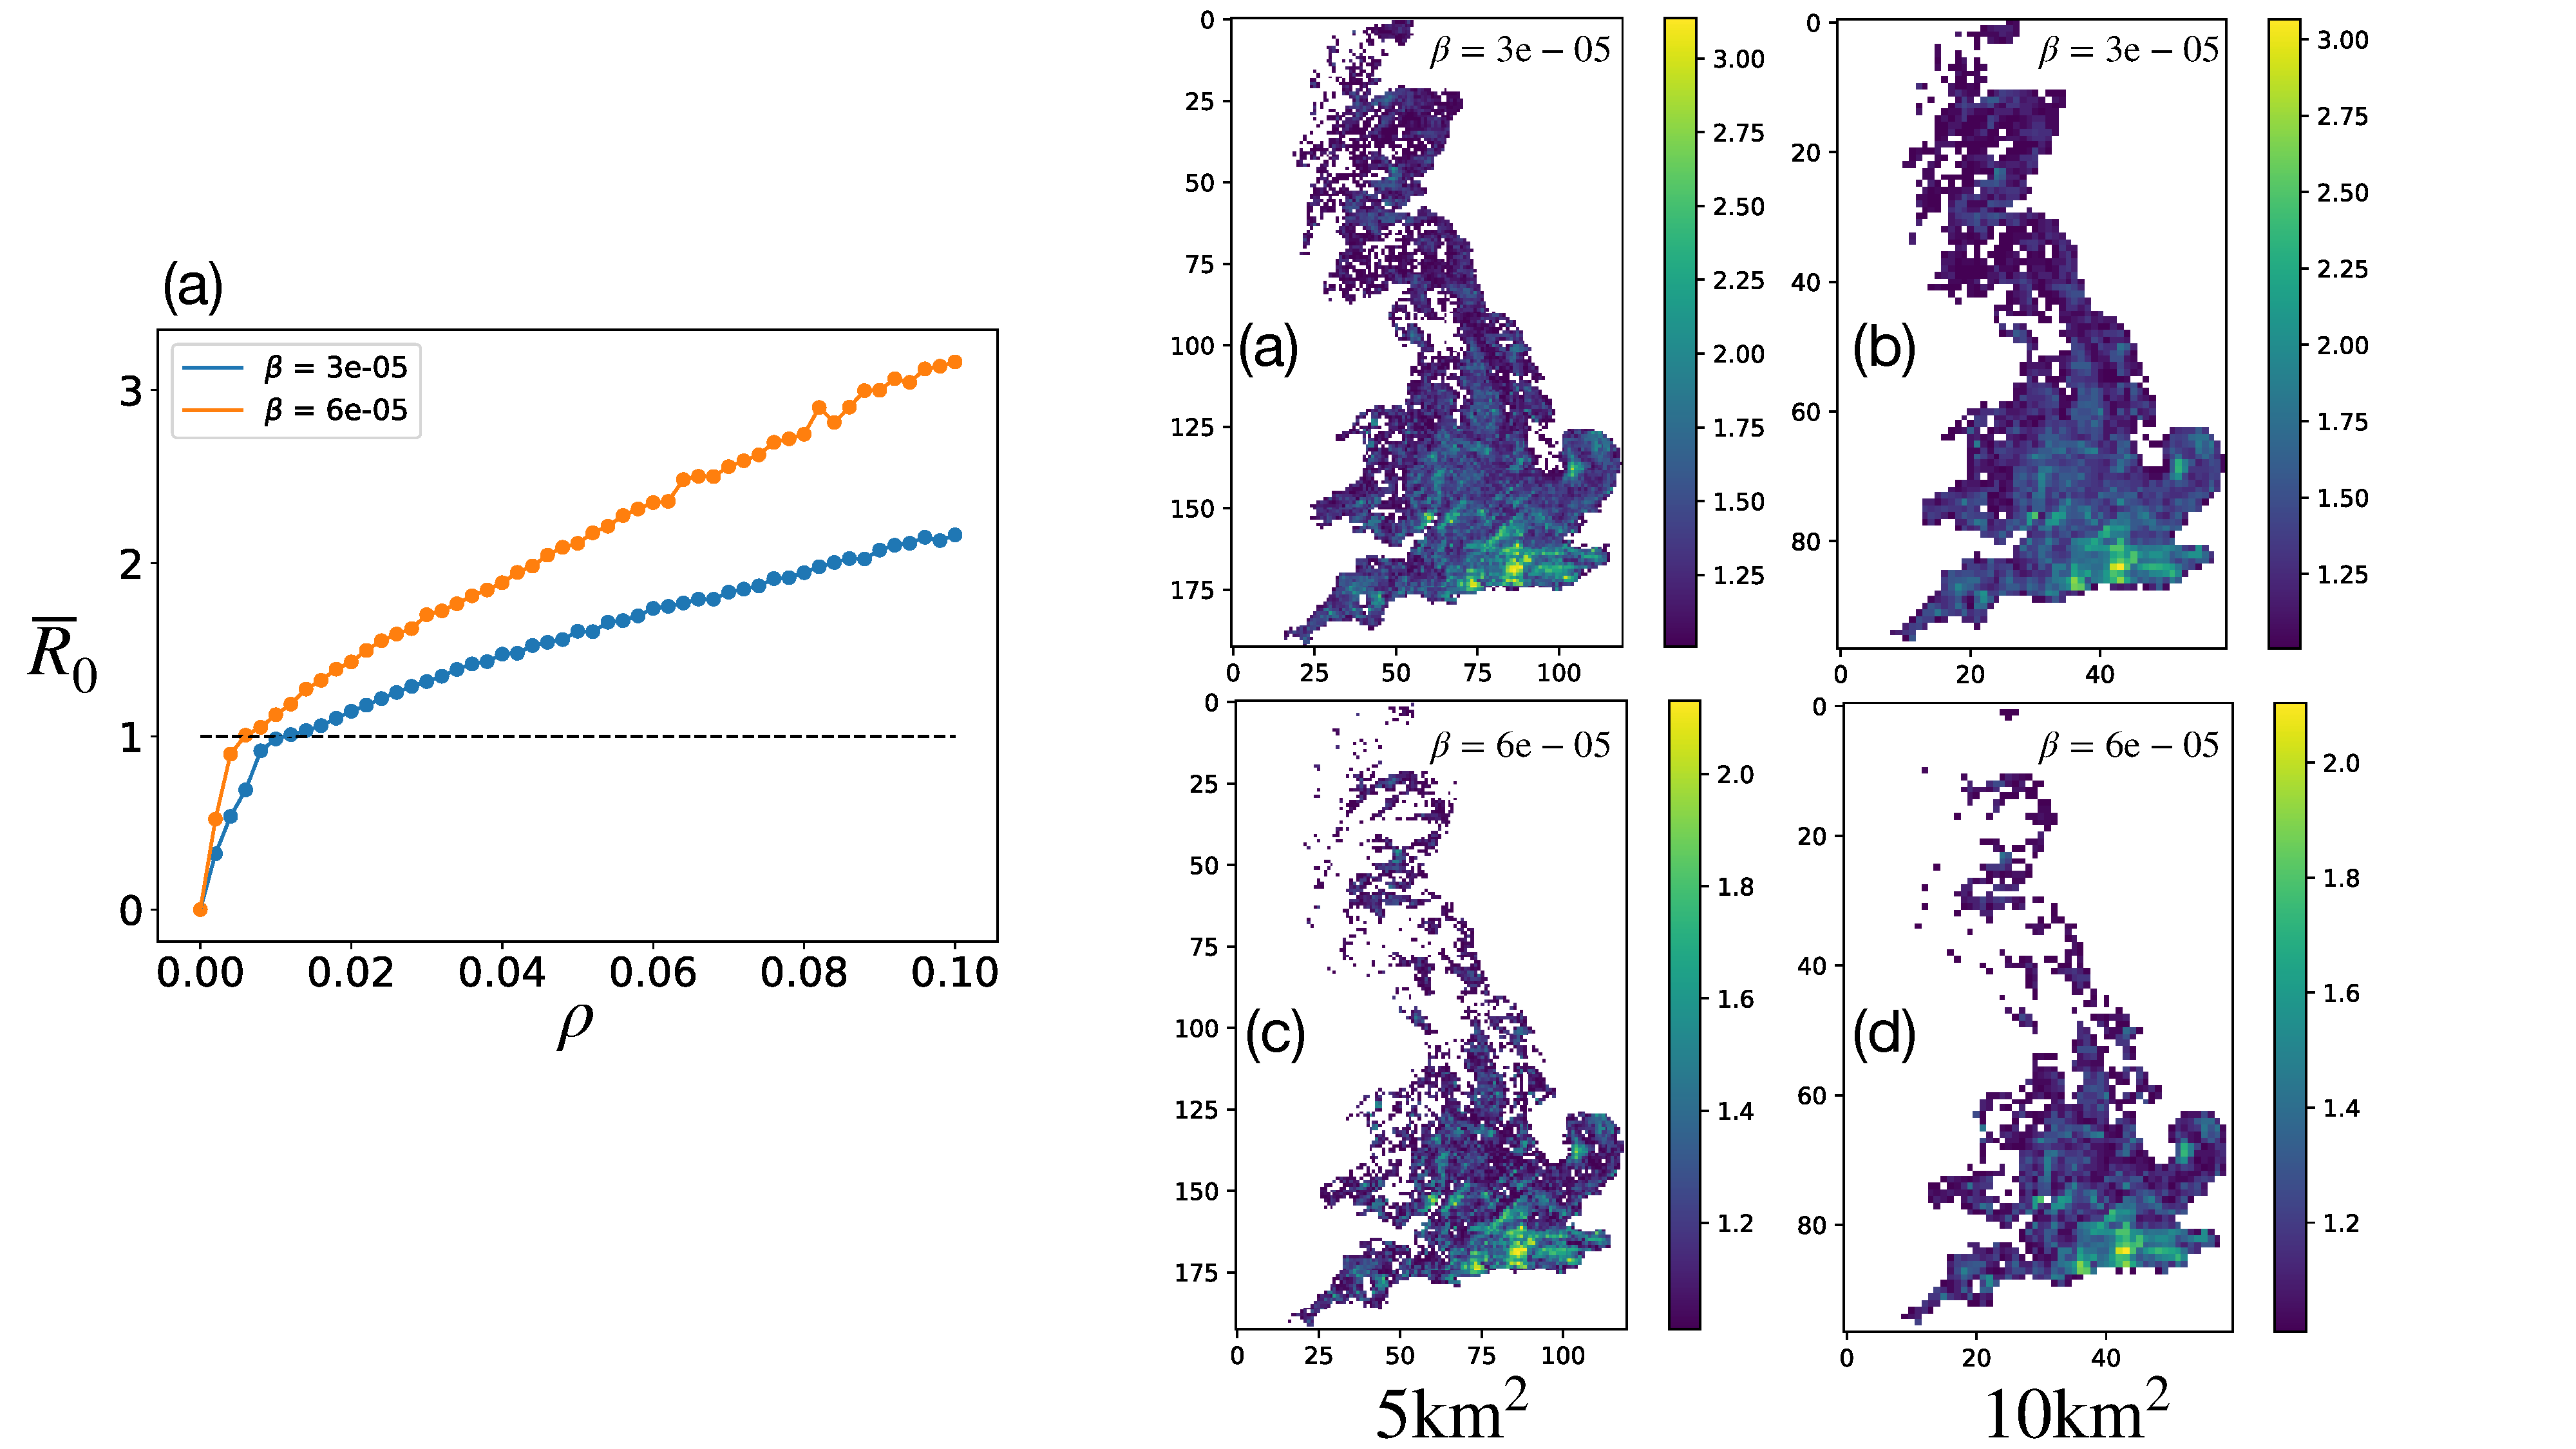
\includegraphics[scale=0.25]{chapter6/figures/fig4.pdf}
%       \caption{(a) Ensemble-averaged $R_0$ between two values of $\beta$, for Gaussian dispersal of $\ell=1.6\mathrm{km}$. (a-b) $R_0$-map for $\beta=3\mathrm{e}-05$, coarse-grained at $5$, $ 10\mathrm{km^2}$. (c-d) $R_0$-map for $\beta=6\mathrm{e}-05$.}
%     \label{fig:uk-mapping}
% \end{figure}

% % Linking R0 clusters to percolation theory
% The structure of connected $R_0$-clusters can be considered through the lens of a `\textit{percolation-like}' theory: if the $R_0$-map were homogeneous, a minimum number of susceptible (or `open' in percolation theory) positions defines a critical density. At the critical density, a `spanning' cluster is realised and percolates through the domain. In Figure\ref{fig:uk-mapping}(b), this picture is complicated by heterogeneity. Subsequently, we found connectedness inside a given cluster could depend on just a small number of `connecting points' which if removed, thinned below $\rho_c$, would lead to significant fragmentation and divide the cluster\footnote{An analogy to this idea can be found in the study of `conductive-insulator' percolation networks, with so called `\textit{hot-bonds}'. If broken, a \textit{single} hot bond can prevent the whole system from conducting \cite{RevModPhys.45.574, Herrmann_1984, hot-bond}. Although, in our analysis, a generalisation of this analogy is presented to include a set of \textit{multiple} hot-bonds.}.\\

% \textcolor{red}{Strictly speaking, the comparison with percolation theory breaks down on account of clustering in the $R_0$-map. That is, the susceptibility of a given pixel is likely dependent on its neighbours $R_0$-value. This contradicts classical percolation theory where lattice points are not correlated but exist independently of one another\textemdash much like the random-homogeneous distribution of trees presented in Section \ref{section:sgm-expo}. We precede by describing how these findings can be used to achieve efficient regional containment of an epidemic.\\}

\section{Optimal fragmentation of $R_0$-maps}

% Each cluster (denoted by $\mathbf{C}$) detected in the $R_0$-map represents a connected network of susceptible Ash where pathogen survival and spread is possible. The shape of each cluster is constrained by landscape topography and geography. If no control is attempted, all trees within a cluster are put at risk if one point in the cluster becomes infected. Given this, a control strategy is formulated by noting that removing specific positions of Ash (or breaking critical `links') via selective tree felling would efficiently break the cluster into two fragments. A technical explanation of the fragmentation algorithm is given in Appendix B.\\

% Cluster fragments define two disconnected `sub-clusters' (named $\mathbf{C_1}$ and $\mathbf{C_2}$). This eliminates risk for trees inside one sub-cluster and accomplishes control by regionally containing an epidemic inside a `confining cluster'. Ash trees inside the confining cluster are assumed to be removed by the pathogen while Ash trees inside the remaining sub-cluster survive and remain susceptible. If the number of felled trees is low in comparison to the number saved, then efficient control is achieved.\\

% The notion of fragmenting a cluster $\mathbf{C}$ into two sub-clusters $\mathbf{C_1}$ and $\mathbf{C_2}$ may be repeated $N$ times to produce a set of disconnected sub-clusters. After each fragmentation, sub-clusters were ranked according to the Ash population size they contained. This allowed the largest sub-cluster to be targeted in the next iteration. \textcolor{red}{Figure X} shows the largest cluster identified in the $R_0$-map (named $\mathbf{C_T}$) iteratively fragmented $N=5$ times culminating in six disconnected sub-clusters, depicted as the colour-filled regions from orange-green. The zoomed inset of $\mathbf{C_T}$ highlights the critically-connecting links found during each fragmentation.\\


% We assume the average Ash tree in the population covers an area of $\mathrm{25m^2}$ (giving a maximum of $400$ trees per hectare of canopy cover \cite{ash-tree2, ash-tree1}). Combining this assumption with the data permits us to estimate the number density of Ash trees per point and subsequently the population size of Ash contained inside each sub-cluster. Additionally, an estimate towards the number of felled trees can be formed, thus giving insight into the scale of resource expenditure. This is achieved by first finding the difference between $\rho_c$ and the density values of critical links (i.e. the level of required density reductions), then multiplying this by the number density.\\

% \textcolor{red}{Figure \ref{fig:result-cluster-reductions}(b)} shows the maximum sub-cluster population size in blue alongside the estimated number of trees needed to be felled in red. The largest sub-cluster continually decreased over $N=30$ iterations of fragmentation. Size reductions occurred more rapidly at first, starting from $\mathrm{3.5\times 10^7}$ trees and decreasing to $\mathrm{1.1\times 10^7}$ trees within $5$ iterations. By $N=30$, the rate of sub-cluster size reductions leveled off suggesting fragmentation in the field may tend towards diminishing returns on control efficiency. That is, larger values of $N$ produce smaller changes in the number of saved trees in proportion to the expenditure of resources needed to fell trees. This is demonstrated when the red and blue lines begin to approach each other, attaining comparable values.\\ 

% \textcolor{red}{Figure \ref{fig:result-cluster-reductions}(c)}, sub-cluster size reductions in $\mathbf{C_T}$ are shown alongside the $2^{nd}$ and $3^{rd}$ largest $R_0$-clusters on a log-log plot\textemdash from solid blue through to green. The straight lines indicate a power-law. The sub-cluster size reductions were fitted to a power-law of the form $f(x) = ax^{-k}$, shown by the corresponding dashed lines. Fitted parameter values of $a$ and $k$ represent the initial cluster population size and rate of decrease respectively. Importantly, all sub-cluster size reductions demonstrate an exponent of $k\sim 3/4$. In addition to the Ash species shown here, Conifer (\textit{Pseudotsuga menziesii}) and Beech (\textit{Fagus sylvatica}) were given by \cite{hill.data} and were used comparatively to test fragmentation. For each species considered, all iteratively fragmented clusters had similar exponent values, $k\sim 3/4$.\\


% \subsection{Towards epidemic control}
% % Main results figure 7
% Regional containment as a strategy of epidemic control was tested by considering outbreaks from different epicenters inside the target cluster $\mathbf{C_T}$. Starting from an epicenter, epidemic containment can be achieved in a variety of ways. \textcolor{red}{Figure \ref{fig:scenario-expo}} demonstrates this for a single epicenter marked by the black cross. The number of fragmentation iterations is varied from $N=1$ to $N=30$. For each step $N$, we identify which critical links, shown in red and denoted as $F$, should be felled below $\rho_c$ in order to define a confining sub-cluster around the epicenter. The population of saved Ash, illustrated in light grey, remains in state $S$ while all trees inside the confining sub-cluster, shown in dark grey, are assumed to transition into state $R$. By assessing the number of trees saved against the number of trees felled we can define a `payoff' ratio as $N_S/N_F$.\\

% A set of epicenters were defined in $\mathbf{C_T}$ (by identifying the center of mass for each sub-cluster when $\mathbf{C_T}$ was iteratively fragmented $N=30$ times). From $31$ different epicenters and $30$ iterations, $930$ containment scenarios were simulated. For some epicenters, typically in close proximity, containment looked identical up to $N$ iterations before a different payoff ratio was registered. Subsequently, less than $930$ unique data-points between $N_S$ and $N_F$ were found\textemdash shown in \textcolor{red}{Figure\ref{fig:result-culling-efficiency}}.\\

% The payoff ratios determined from the top $50$ performing containment scenarios were then ranked and plotted, shown in Figure\ref{fig:result-culling-efficiency}(a) by the blue line overlaid with a coloured scatter plot. For the purposes of our model, the payoff efficiency is shown alongside the corresponding number of felled trees in dashed grey. Payoff efficiencies begin to level off around $\mathrm{10^3}$ involving around $\mathrm{10^4}$ felled trees. In reality, this would be a challenge to accomplish in a reasonable time-frame. Figure\ref{fig:result-culling-efficiency}(b) shows a scatter plot of all the data, $N_S$ and $N_F$ are plotted with color corresponding to the payoff. The efficiency ranged over multiple orders of magnitude up to a maximum efficiency of $\mathrm{10^6}$. The top left quadrant of Figure \ref{fig:result-culling-efficiency}(b) represents viable scenarios where containment felling could be pragmatically implemented by policy makers with the greatest efficiency.\\

% A small number of exceedingly high payoff results were found. In Figure\ref{fig:result-culling-efficiency}(c), the top three ranking payoff scenarios are illustrated on the same map and reinforces the intuitive notion that epicenters around edge positions can be most efficiently contained. The zoomed inset highlights just $\mathrm{2\times 1km^2}$ Ash patches located at a single point of contact for the top ranked sub-cluster. Critical links for the best performing scenarios were all found in lower-density regions within the $R_0$-cluster and were easily fragmented with a low number of felled trees. This highlights the possibility that fragmentation is most easily achieved with tree felling through critically linking regions and demonstrates how regional variation in host density can be exploited for efficient control. 

\section{Chapter summary}

% Where we consider spatial structure and others have not
% - In this chapter, we focused on disrupting local-level dispersal by implementing control at landscape-level.
% -  In this chapter we undertook the ambitious task of scaling up a small-scale model, to large spatial distances covering GB, and developed a new approach to controlling the spread of disease.
% - introduce the regime of pathogen spread we are interested in, we are not modelling continental long-range spread via upper atmosphere, nor are we interested in long-range human trade networks. We are interested in dispersal at the local level whereby passive means of wind, soil and or insects/animals. 

These results are focused toward help policy makers implement informed decisions, about \textit{where} to control the spread of disease, based on spatial arguments, when budgets are low\textemdash as noted by \cite{time-varying-infectivity}. Our approach of spatially scaling small-scale epidemiological principles was conducted through computational, opposed to analytical, means. 

The article published by \cite{time-varying-infectivity} indicates the possibility of \textit{preferentially} controlling an area based on the final-sized epidemic. It goes without saying that areas of land that have the largest final sized epidemic are likely the most density populated. However, we outline the possibility it might be more beneficial to preferentially control an area based on its spatial location and how it couples to to neighbouring areas.

% The scaling up of our model
The scaling up of our model resembles a metapopulation model, now commonplace when modelling plant-based epidemics, but crucially our large-scale model is not dynamic. A dynamic large-scale model is indeed useful for the prediction of time-scales and the movement of disease-fronts movement; however, we suggest they might be at best less useful for optimised large-scale control, and at worse, nicely complemented by the approach we develop.

If early data through a particular region, with known data, was collected, it would be a relatively short step to fit the dispersal model and scale up the model over large distances given the seemingly simple relation to host density $\rho$.
% At the small scale we have a uniform population. However for larger scales we have considerable spatial heterogeneity.
% spatial-scale and control, over a multi-seasonal pathosystem, have been investigated for sugar beet in the UK, see \cite{doi:10.1146/annurev.phyto.45.062806.094357} for a review.

% On the SEIR model

The cyclic nature of the $SEIR$-type model constructed in this article can also find resemblance in the, well established body of literature, of crop-based epidemics. It is common-place for a field of crops to become infested, then at the end of the growing season be totally eradicated by virtue of harvesting % \cite{time-varying-infectivity} has 
% we contend the SnIEmR model, considered over one sporulation peak, is a simplistic implementation of the SEIR-based model needed to compute an invasion threshold that represent the infection dynamics ash dieback. 
% The SEIR-based model is made more flexible, and can be readily extended or adapted to incorporate more biological realism, by virtue of splitting the E and I into multiple compartments\textemdash this is frequently done in human and animal-based models \citations..

%- Although the main result of our work was conduced over one sporulation peak, or life-cycle of ash dieback, splitting the model into various compartments was a useful and necessary step towards developing accurate large-tree species. reference  \cite{https://doi.org/10.1111/ppa.12894} alludes to multiple exposed periods being useful

%- A quantity of interest that appears frequently in the literature is the initial growth rate $r$, that is the density-independent growth at the start of any epidemic.
% See \cite{ferrandino2012time} for a review on the time-scales and sporulation of plant-based diseases.

% Fitting data to the early phases of an epidemic has been shown to give large differences in the final-size epidemic, or severity \cite{time-varying-infectivity}. However, we are only interested in a pathogens ability to invade and this can be closely approximated by measuring R0 over the fist observation (\see appendix)

% The variability between the particular life-cycle history followed by hosts is thought to be an important factor to consider\cite{ferrandino2012time}, and we intentionally neglected this for the purpose of simplicity...

% Accurately modelling time-varying infectivity is difficult \cite{13-challenges}, and as such, we opted for parsimony.

% Main assumptions in the method: 
% 1) Assumptions about dispersal
Dispersal over small spatial-scale is thought to predominately occur passively through wind, however other means of dispersal exist such as soil and or insects. There are many pathways a pathogen can use to spread through a landscape, including long-range dispersal, mediated through either human-trade networks %
\cite{hulme2009trade, banks2015role, chapman2017global} or dispersal in the upper atmosphere \cite{westbrook1999atmospheric, isard2005principles}.  

% We assumed some regions can sustain an epidemic and some cannot, we assume that $R_0>1$ is the threshold separating these regimes.

% 2) Assumptions about R0
To our knowledge, $R_0$ has not been estimated for Ash dieback, or indeed for any large deciduous tree species, unlike for some crop-based pathogens \cite{segarra2001epidemic}. The lack of $R_0$-estimates made it hard to scrutinize which $\beta$-valued $R_0$-map would be likely to reflect reality. This gap in the body of literature is hardly surprising given the complexity of measuring time-varying infectivity rates \cite{13-challenges}. Thus, as it stands, our results hint-towards the utility of landscape-level control but come short of definitive proof.

% Looking at \cite{R0-perc-ref}, it makes me think our notion of $R_0$ is pretty simplistic. We only measure the local-level $R_0$. We do not consider $R_0$ from patch to patch. What scale we measure $R_0$ has a huge impact on what the result is. Could we rank land-patches not only on there local $R_0$ level, but also on the impact they have on there immediate neighbours ? This would, in theory be an improvement to the clustering algorithm.

% Improvements to the model:
% 1) The algorithm
% The algorithm to target not only the critically connecting patches, but also find fragmenting lines which minimise risk at the landscape-level ? Incorporating the local impact a particular patch may have on its neighbours.
% 2) Multi-year R0 analysis
% However, we .... xyz cover all basis of using a one-season approximation. <- this leads to a risk-based argument in which we could capture a 2nd-order R0 which does, xyz. We mainly interested in a pathogens ability to invade. 

% Analysis was aired towards simplicity, a more expansive study with e.g. more sophisticated sporulation functions could be the subject of future work.

% The most important message of our work was...
% The spatial and temporal scale of the control-strategy should match intrinsic spatial and temporal scale of the invasion. <- Hence R0 measured over one season. 


% our modelling approach and results are in their infancy,  

% Last remarks and future modelling work:
To our knowledge, there is a surprising lack of spatio-temporal ADB models exist in the literature, probably because of the significant challenges involved in containment. Although our findings are far from complete, it suggests the spread of ash dieback, between spatial locations, could be reduced by preferentially targeting sites to minimise epidemiological connectivity. Not surprisingly, more work will need to be done to ascertain the degree to which this strategy could impede the spread. 

% Crucially, future work will involve integrating LDD mechanisms into the model in order to understand the relative importance long vs local distance dispersal. We may speculate about the relative importance looking at figure x, whereby the maximum distance spread in season due to local-scale spread is xm/year, in stark contrast from the observed spread of 40-60km/yr.

% We cannot overstate the importance of LDD, and it is hard to say the degree to which targeting the local dispersal mechanism alone will inhibit the spread. We will revisit this question in future work, however, we contend that preferentially targeting diseased trees based on spatial location.....could help control epidemics with greater efficacy. 

% We may speculate how our result could aid the effort of choosing where to re-plant ash stands genetically engineered to be less susceptible; if re-planting efforts were undertaken in certain location.... <- speculative

% We may speculate about how persistent ash dieback would be, even if a large-scale control effort was undertaken

% There is evidence to suggest regional variation in mortality due to ash dieback \cite{stocks2017first}, this could be incorporated into the model...

% Our results support the call for more research to be undertaken into multi-scale dispersal, 

% Recently, it has been suggested that the dispersal-kernel of wind-borne pathogens might follow a scaling law \cite{https://doi.org/10.1111/jbi.13642}. The significance of such a finding would allow us to analyse the $R_0$-maps over much more flexible spatial scales. % Explain.

% This sentence is wrong, the cited paper makes an argument for the spatially-scaling up of dispersal kernels, which happens to still be useful paper to cite, re-phrase and re-frame accordingly.

% see \cite{ash-dieback-costs}, and the references therein (methodology excel spread sheet S1), for mortality references the latest findings suggest a mean mortality rate of 95%.





% 7) A method of control at the landscape level 
% ------------------------------------------------------------------------------
% A primer on continuum models and how this relates to the work we have done
% 1) Introduce logistic growth and diffusion
% 2) Introduce FKPP in all its glory .
% 3) Show one and two d spread
% 4) Couple to the sub-grid, what this says about the sub-grid...
% 5) Talk about growth rate-alpha and growth rate of sub-grid... an assumption about mixing and SIR <--         appendix territory
% 6) Show `toy model properties in alpha and d' get realistic looking spread...
% 7) Show realistic spread and give a primer to things which could be done.
% 8) Talk about alternate more, non-linear models and consult Rammile...
% ------------------------------------------------------------------------------

\chapter{Continuum Models of tree diseases}
The typical approach is spatial-$SIR$ \textcolor{red}{REVIEW SPATIAL SIR}, however, tree disease is localised and will does not fit well to an $SIR$ model\textcolor{blue}{CITE MASTERS PROJECT (unpublished)}. %whose  Masters project is this ??
As such we opt for 

\textcolor{blue}{Lit-review: 1) PDE/continuum models for disease 2) reaction-diffusion models}
\textcolor{red}{This chapter takes a different modelling approach from the ones seen so far. %
A continuum approach, formulated on reaction diffusion equations, is used to describe the spread of disease. %
The aim of this Chapter is to offer a first approximation towards a continuum model. %
PDE models have been  studied rigorously in the context of biological waves, disease and population dynamics. %
The most basic reaction diffusion equation is the Fisher equation, also known as the the Kolmogorov–Petrovsky–Piskunov equation or FKPP equation for short. %
FKPP equation. This equation makes for an attractive off-the-shelf model, with known solutions, well-studied behaviour and a simple form involving both logistic growth and diffusion-based propagation.}                                                


\textcolor{red}{Firstly we establish the two components of reaction-diffusion, that being logistic growth and diffusion, in separate models. Then we proceed to show how diffusion coefficients can be informed by the non-local dispersal model and data sets presented in Chapter \ref{chapter:regional-containment1} }. We explored how modelling individual trees within a map covering GB  was computationally infeasible. Another approach that works around this problem is to use a continuum model. Using a continuous model in the form a partial-differential equation permits the averaging-out of previously discrete quantities, such as the number of infected trees or the concentration of the unit of infected  trees.

 Ahybrid modelling approach was developed, both flexible and generalisable, based on a Monte Carlo sub-grid model at resolution 5m and a reactive-diffusive PDE model at resolution 1km. %
 The Monte Carlo sub-grid model uses a non-local compartmental SIR model and is shown to demonstrate travelling wave-like behaviour when ensemble-averaged. %
 The reaction-diffusion system chosen is the FKPP equation, as the simplest model that  demonstrates the propagation of travelling waves and logistic growth of the pathogen. From simple epidemiological input parameters travelling wave-speeds of the sub-grid are pre-determined and mapped to diffusion coefficients informing the FKPP equation. %
 The FKPP then simulates a pathogen spreading over GB. This framework relies on a species abundance distribution. %
 Although efforts are being undertaken to attain high quality abundance data over large distances, at present no such data is publicly available. %
 For this reason we use modelled abundance data of GB tree species. This chapter contributes in  developing resalable large-scale epidemic models based on small scale epidemiological principles. %

\section{PDE modelling for tree disease}
PDE models are useful because they can model averaged, or smoothed, quantities such as the number of infected trees at each point in time and space. Reaction-diffusion (RD) PDE's  have been used extensively for the purpose of epidemic modelling in space and time, \textcolor{red}{see Chapter \ref{chapter:lit-rev}}. The simplest description that can be used to model the spread of a non-static pathogen comes in the form of a reaction-diffusion PDE. That is, the Fisher-Kolmogorov (FKPP) model. The FKPP model has well-studied solutions that exhibit travelling waves. The FKPP model is based on the diffusion and logistic growth of a given quantity or field $u$. %
Together, the growth and diffusion of a quantity give rise to a self-propagating wave that spreads outwards in time and maintains the same shape.\\

\subsection{The FKPP model}

In one spatial dimension, the FKPP model is given by:
\begin{equation}
\label{eq:fkpp-expo}
    \frac{\partial u}{\partial t} = \mathcal{D}\frac{\partial u}{\partial x} + ru(u - 1)
\end{equation}
where $\mathcal{D}$ is a diffusion coefficient measured in units $\mathrm{m^2 t^{-1}}$ and $r$ is a growth constant (or rate) with units $t^{-1}$. %
This model assumes logistic growth and diffusion of the field $u$. In the context of modelling the spread of disease through a population of trees, the field $u$ constitutes the `concentration' of pathogen at a particular point. %
When the pathogen concentration reaches the maximum value of $1.00$ all susceptible tissue is taken as infected. This is an assumption that could lead to an over-estimation of disease  as pathogens are unlikely to infect all susceptible units of trees in a given region \cite{neher1992underestimation}. %
However,  modifications, for example \ref{eq:fkpp-expo} are possible. One example is seen with the inclusion of a carrying capacity $K$\footnote{A carrying capacity could easily be included into the model given in the logistic growth term $(\frac{u}{K} - 1)$ The field $u$ is then interpreted as a raw number of infected. \textcolor{red}{SEE REFERENCE...}}, here , I keep using   the most basic variant.

\begin{figure}
    \centering
    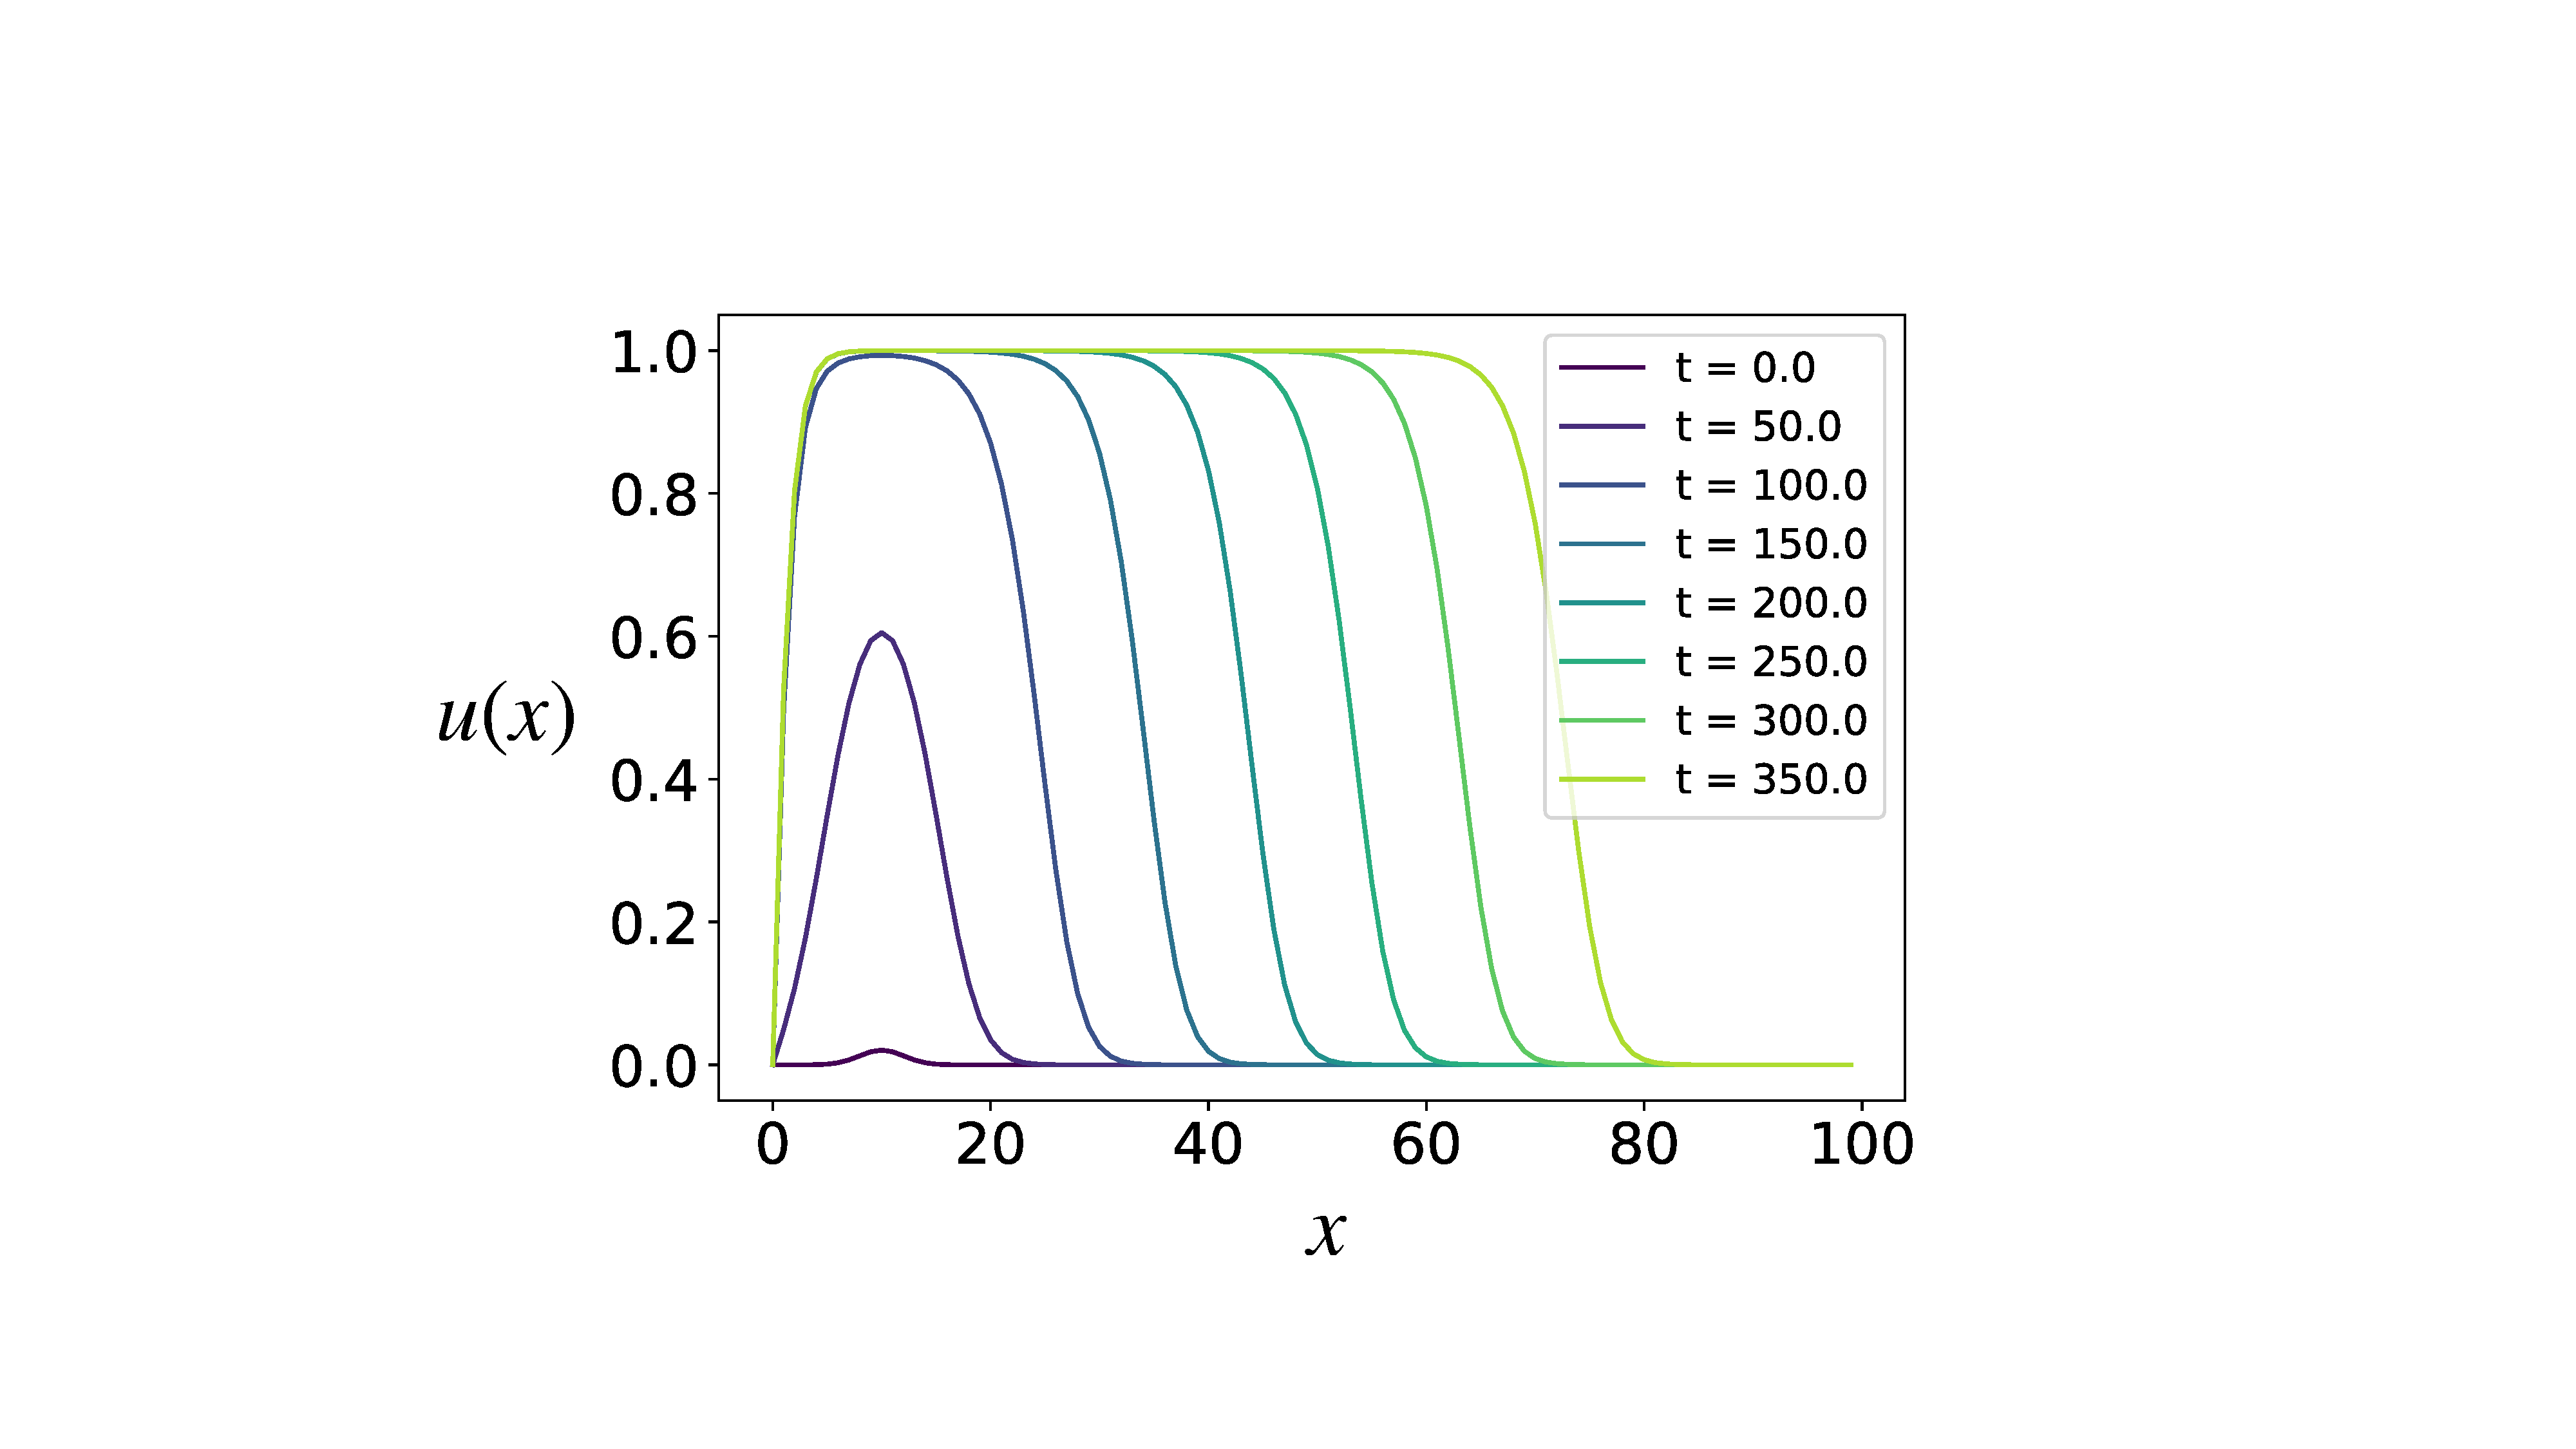
\includegraphics[scale=0.25]{chapter7/figures/figure1xy.pdf}
    \caption{A simulations of the FKPP model for $r=0.10$ and $\mathcal{D}=0.10$ in one spatial dimension. A non-zero field value is initialised at $x=10$ at time $t=0$. Uniform growth and diffusion give rise to a wave-front that propagates with constant speed.}
    \label{fig:fkpp-expo1D}
\end{figure}


\begin{figure}
    \centering
    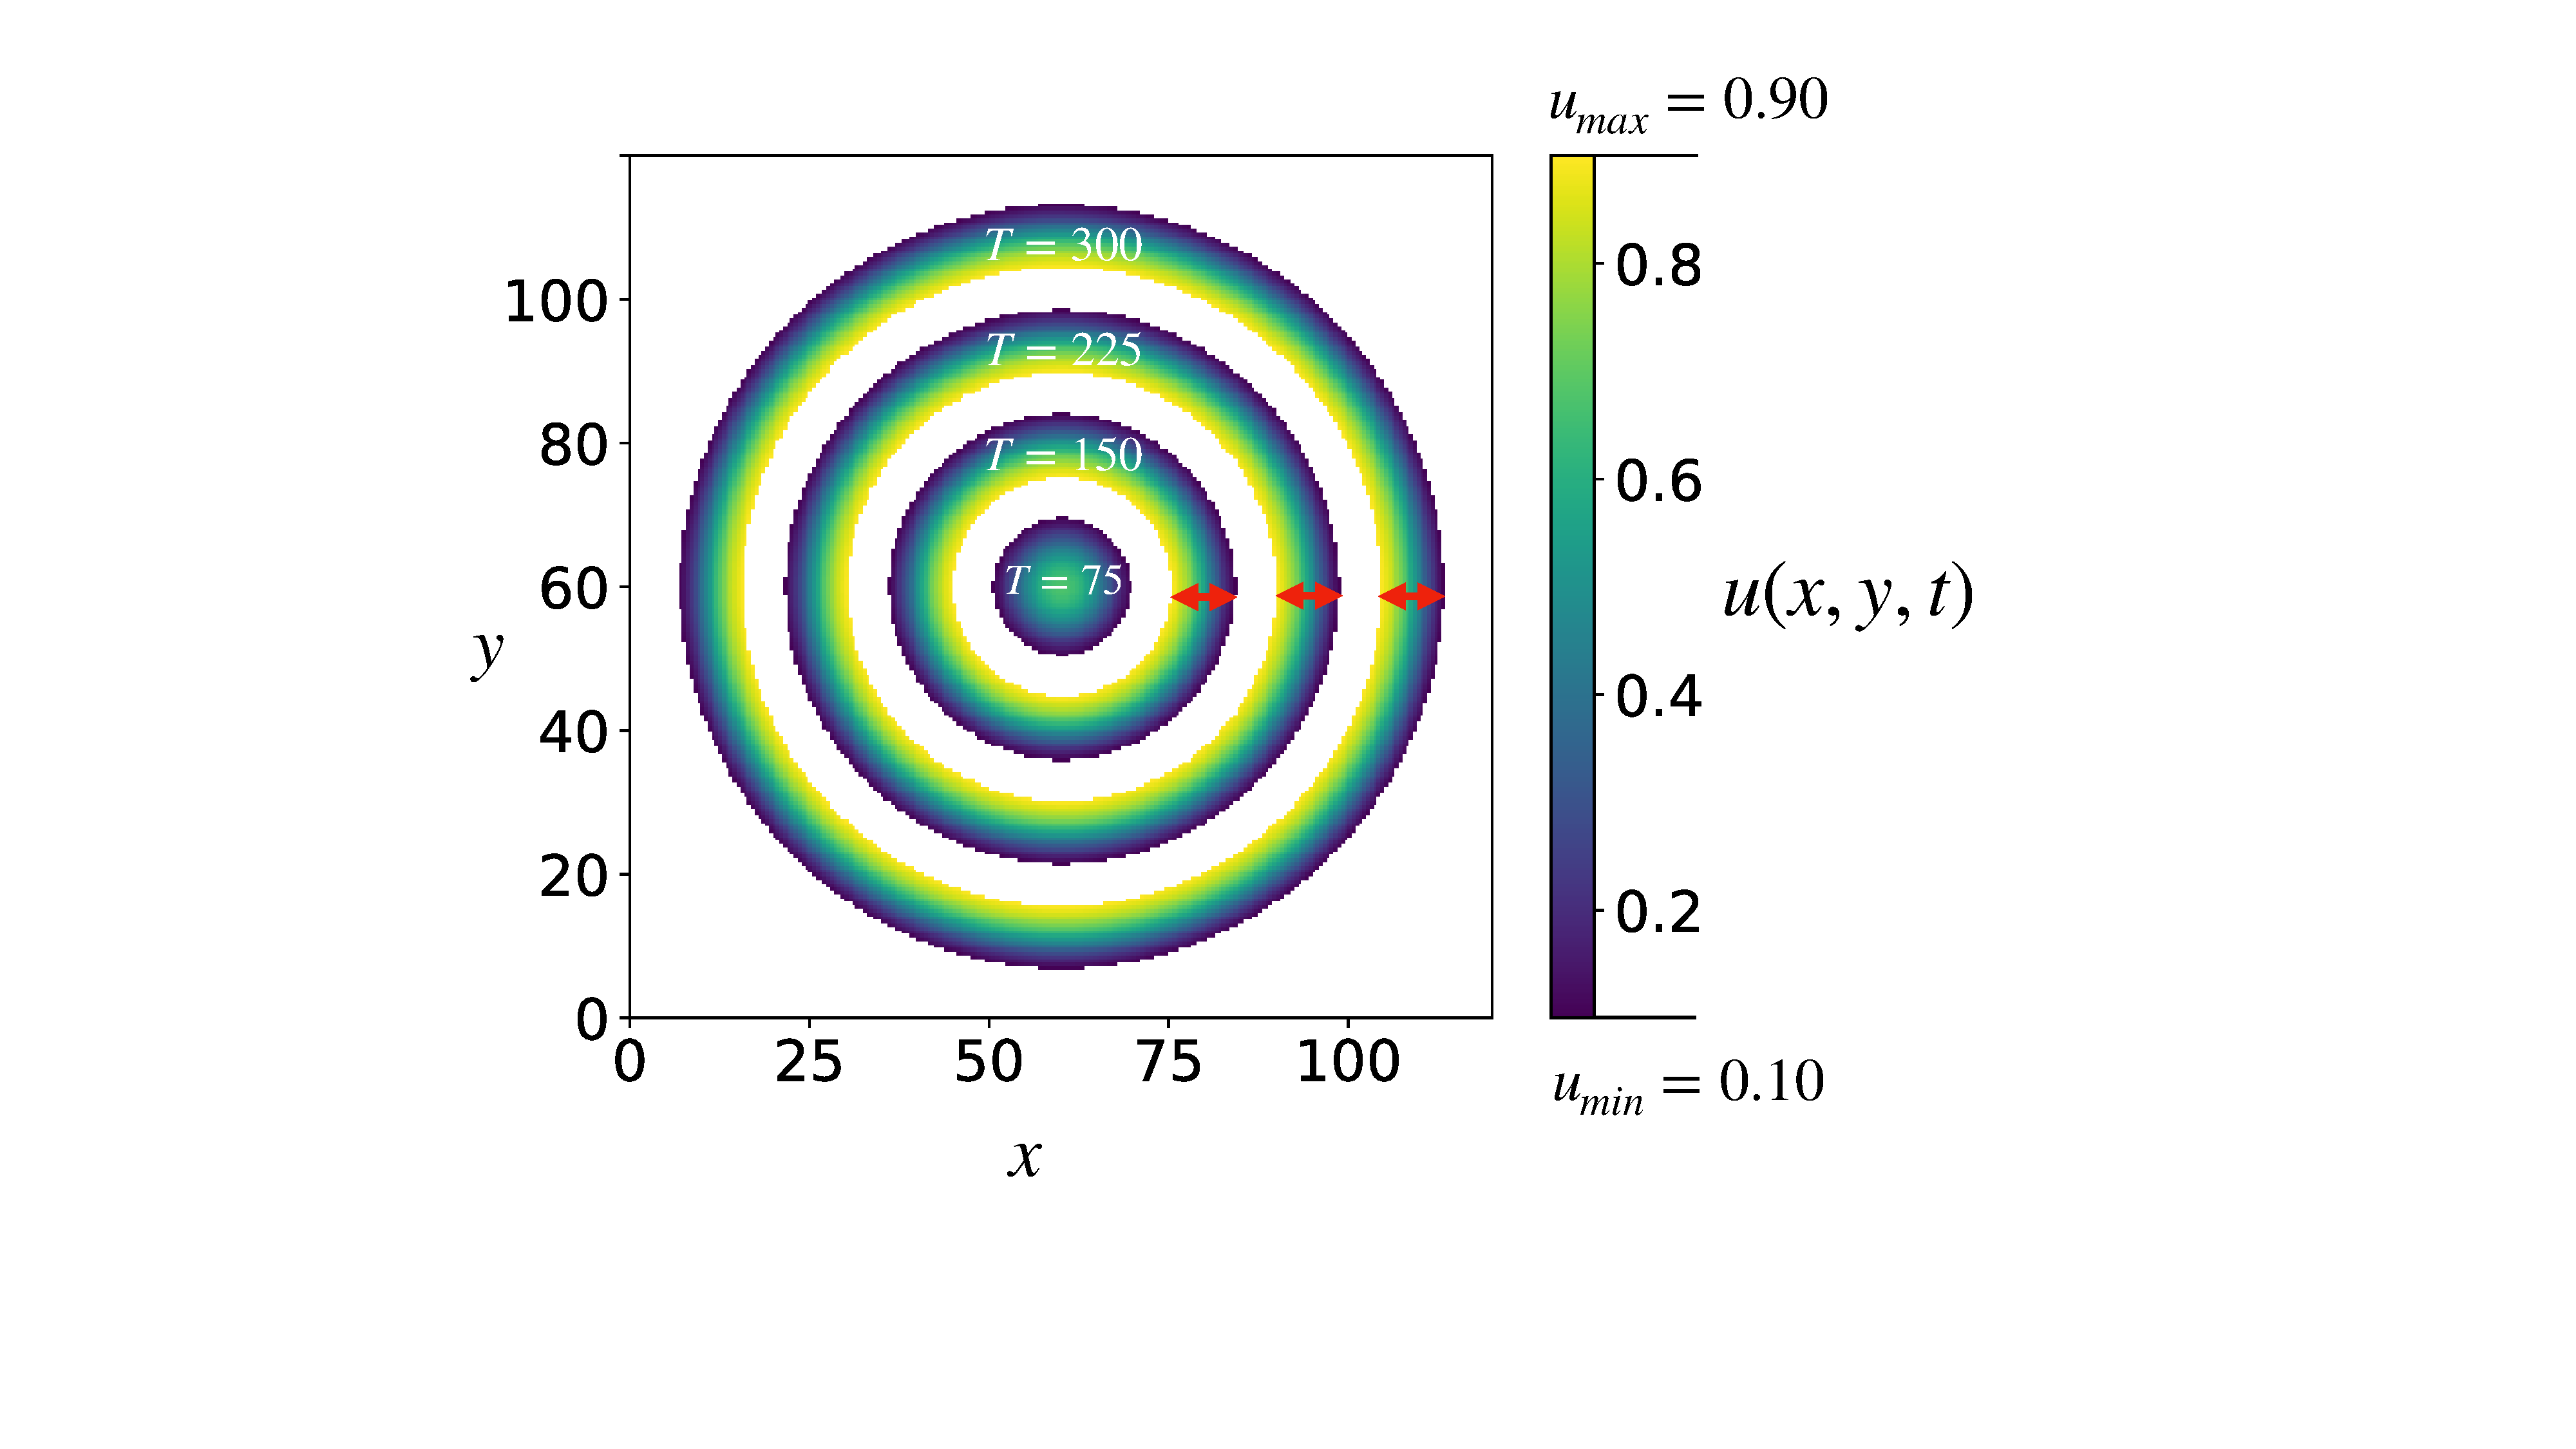
\includegraphics[scale=0.25]{chapter7/figures/figure2x.pdf}
    \caption{A simulation of the FKPP model wave-front for $r=0.10$ and $\mathcal{D}=0.10$ in two spatial dimensions. A non-zero field value is initialised at the domain center at time $t=0$. The field values $0.10 < u < 0.90$ are used to trace out the evolving wave-front and ascertain the speed of propagation. Uniform growth and diffusion give rise to a symmetric front that propagates with constant speed $v=0.200$.}
    \label{fig:fkpp-expo2D}
\end{figure}

Figure \ref{fig:fkpp-expo1D} shows the simulated FKPP model in one spatial dimensions using a forward-time centred-difference (FTCD) scheme, see Appendix \ref{a:pde}. Constant diffusion and growth coefficients, $r=0.05$ and $\mathcal{D}=0.10$, lead to a travelling wave that propagates in the positive $x$ direction with constant speed. The travelling wave solutions of Eq \ref{eq:fkpp-expo} can be shown to advance with speed:
\begin{equation}
    \label{eq:fkpp_vel}
    v \geq v_{min} = 2\sqrt{r\mathcal{D}}
\end{equation}
where $v_{min}$ is the minimum wave-speed admitted by the front, see \cite{murray1993mathematical} for a complete derivation. %
For the purpose of modelling an epidemiological wave, it suffices to take $v\approx v_{min}$ as an approximation to the speed of propagation. %
Using Eq \ref{eq:fkpp_vel} the predicted wave-front speed in Figure \ref{fig:fkpp-expo1D} is given by $v=0.200$. %
The numerical stability of simulations is ensured provided that the Courant–Friedrichs–Lewy (CFL) condition is met\cite{cfl-condition}. %
In the case of the FKPP model, the CFL condition is given by:
\begin{equation}
    \mathcal{D} \frac{dt}{dx^2} < \frac{1}{2}
\end{equation}
where $dx$ and $dt$ represent the discretized domain and time-steps respectively. %
The observed wave-speed of simulations can be calculated by %
tracing the time-evolution of the wave-front mid-point (ie. where $u(x) = \frac{1}{2}$). %
After initial transience, the wave-front in Figure  \ref{fig:fkpp-expo1D} was found to evolve with speed $0.199$ with discretized steps $dx=0.50$ and $dt=0.10$. %

The two dimensional variant of the FKPP model is similarly given by:
\begin{equation}
    \frac{\partial u}{\partial t} = \mathcal{D}\nabla u + ru(1 - u)
\end{equation}
where the field $u$ is now a function of both $x$ and $y$. %
Strictly speaking, Eq \ref{eq:fkpp_vel} is only valid for a one dimensional domain, however, it was found to offer a close approximation for the two dimensional wave-speed,  \textcolor{red}{SEE APPENDIX \ref{a:pde}}. %
\textcolor{red}{Murray, find that curvature 1/r approximation, eq 6.2 only valid for a straight front}. %
Using a FTCD scheme with steps $dx = 0.50$ and $dt = 0.10$, the measured front-speed of the field $u$ in Figure \ref{fig:fkpp-expo2D} was found to be $v=0.189$. %
Using smaller discretized steps of $dx = 0.25$ and $dt = 0.05$ the front-speed can be improved to $v=0.200$ to three decimal places.

Crucially, $\mathcal{D}$ and $r$ control the thickness of the wave front, shown by the red arrows in Figure \ref{fig:fkpp-expo2D}. %
Approximately, the length-scale of the wave-front $\ell_{w}$ can be informed by the quantity $\sqrt{ \frac{\mathcal{D}}{r}}$ (as can be seen by the cancellation of units $\frac{length^2}{t} \frac{1}{t^{-1}}$). %
This can have useful epidemiological implication and is  discussed later on. 

\section{FKPP\textemdash coupling to non-local dispersal model}

The travelling wave solutions of the FKPP model presents a simple starting place to model the spread of disease through a population of trees. %
However, problems arise when estimating the parameter values of $\mathcal{D}$ and $r$ for a particular pathogen (\textcolor{red}{look into lg Plank-formulation and parameter estimates.}). %
A step toward to overcom this problem % what problem?
can be taken by looking towards the non-local dispersal model established in Chapter \ref{chapter:regional-containment1}. %
Specifically, the FKPP model can be informed by the non-local dispersal model via Eq (\ref{eq:fkpp_vel}).

Given fixed growth rates, the non-local dispersal model can be used to inform diffusion coefficients for the FKPP model. %
Re-arranging Eq (\ref{eq:fkpp_vel}) for the diffusion coefficients leads to $\mathcal{D} = \frac{v^2}{4r}$ and the %
investigation moves toward ascertaining $v$ from the non-local dispersal model. %
Figure \ref{fig:fkpp-sgm-vel} shows the process of informing diffusion coefficients based on simulations of the non-local dispersal model. 

The Gaussian dispersal model defined in Chapter \ref{chapter:regional-containment1} gives rise to an epidemic wave-front, defining an interface between infected and susceptible trees. %
Figure \ref{fig:fkpp-sgm-vel}(a) depicts such an epidemic wave propagating through a domain of size $2\mathrm{km}^2$ for arbitrary parameters shown. 5
A distance can be calculated by assessing the furthest distance of an infected tree away from the epicenter, at the domain center, in this example shown by the blue arrow. %

Recording the maximum distance for each simulation time-step leads to a time-series. %
Figure \ref{fig:fkpp-sgm-vel}(b) shows the time-series generated for fixed parameters $\ell, \beta$ and five values of $\rho$. %
The vertical dashed lines indicate positions in time where the pathogen reached the domain boundary, this is analogous to percolation, see Chapter \ref{chapter:regional-containment1}. %
If the pathogen reaches the domain boundary, the  simulation is terminated. %
At the end of the simulations the last recorded distance is divided by the elapsed time, in order to form a naive estimate for the pathogen wave-speed.\footnote{There are many metrics that could be used to trace the evolving front, such as, radially averaged velocity, radially averaged center of mass velocity, median infected distance and average infected distance. However, ensemble-averaged simulations approach the same value and as such the maximum distance was chosen for simplicity.} %

As discussed in Chapter \ref{chapter:regional-containment1}, a pathogen with parameters below the threshold can spread for a time before becoming extinct. This leads to a non-zero spreading speed being registered even though parameters are below the threshold for propagation. %
If non-zero wave-speeds are registered, inferred diffusion coefficients would also assume non-zero values and given the FKPP model levels of infection would logistically increase to unity. %
This is clearly unrealistic for parameters below the threshold for propagation and presents a issue that needs to be addressed and  resolved by considering the wave-speed \textit{multiplied by} the probability of percolation, shown in Figure \ref{fig:fkpp-sgm-vel}. %  

Given stochasticity in the time-series, more reliable estimates for the wave-speed can be generated by ensemble averaging simulations. %
Figure \ref{fig:fkpp-sgm-vel} shows ensemble-averaged results of wave-speed over the parameter space of tree density $\rho$ and pathogen infectivity $\beta$. %
Solid lines show the ensemble-averaged wave-speeds corrected for by multiplying by the probability of percolation. %
Dashed lines show only the wave-speed, without multiplying by the probability of percolation. Dashed lines emphasize regions of parameter space that would be subject to pathogen extinction, pinning these regions to zero keeps the generated diffusion coefficients to zero and constrains spreading in the FKPP model.

Figure \ref{fig:fkpp-sgm-vel}(c) and Eq (\ref{eq:fkpp_vel}) present a mapping function to FKPP diffusion coefficients. %
This relies on fixed growth rates, $r$, and informed tree densities $\rho$. %
As in Chapter \ref{chapter:regional-containment1}, we can use the data-sets reported by \cite{hill.data} to inform tree canopy cover and values of $\rho$ (tree density) over Great Britain. %

Figure \ref{fig:fkpp-diff}(a) shows the diffusion coefficients generated for fixed values $r=0.01\ \mathrm{day^{-1}},\ \beta=0.020\ \mathrm{day^{-1}},\ \ell=25\ \mathrm{m}$ projected onto the Ash tree abundance data from \cite{hill.data}. %
First, each pixel of tree density is mapped onto a predicted wave-speed using results from the non-local dispersal model shown in Figure \ref{fig:fkpp-sgm-vel}(c). %
Each pixel-valued wave-speed is then mapped to a diffusion coefficient using Eq(\ref{eq:fkpp_vel}). %
This paradigm constitutes a continuum-based variant of the sub-grid model presented in Chapter \ref{chapter:regional-containment1}. %
This time however, the model does describe dynamic spread of the pathogen. 

A zoomed $150\mathrm{km^2}$ subset of the diffusion coefficients is plotted in the inset. %
Figures \ref{fig:fkpp-diff}(b-d) depict the FKPP model running with the sub-grid informed diffusion coefficients and a fixed value of $r=0.01\ \mathrm{day^{-1}}$ from years $1, 5, 10$ respectively. %
Initially, a small patch of land $5\mathrm{km^2}$ is infected with a value of $u=0.10$ pathogen occupation. Growth and spread of the pathogen can then be seen to take place in the form of a wave-front.  %

As the field $u$ is bounded between $[0, 1]$, fixing the growth rate to $r=0.01\ \mathrm{day^{-1}}$ approximates a reasonable, %
albeit uninformed, growth rate of a pathogen\footnote{For a fixed growth rate of $r=0.01$, it takes approximately $2$ years for an initially infected field value of $u(x)=0.01$ to attain a final value of $u(x)=0.95$ pathogen occupation.}. %
The final extent of pathogen spread over a $10$ year period is indicated by the double arrow in Figure \ref{fig:fkpp-diff}(d) spanning a distance of $\sim 35\mathrm{km}$. %
From this, we can see that the spreading rate is too small in comparison to a typical epidemic (see \cite{dutch-elm-mismanage} for a discussion on the Dutch elm disease epidemic) and presents a set of problems with the model. %


\begin{figure}
    \centering
    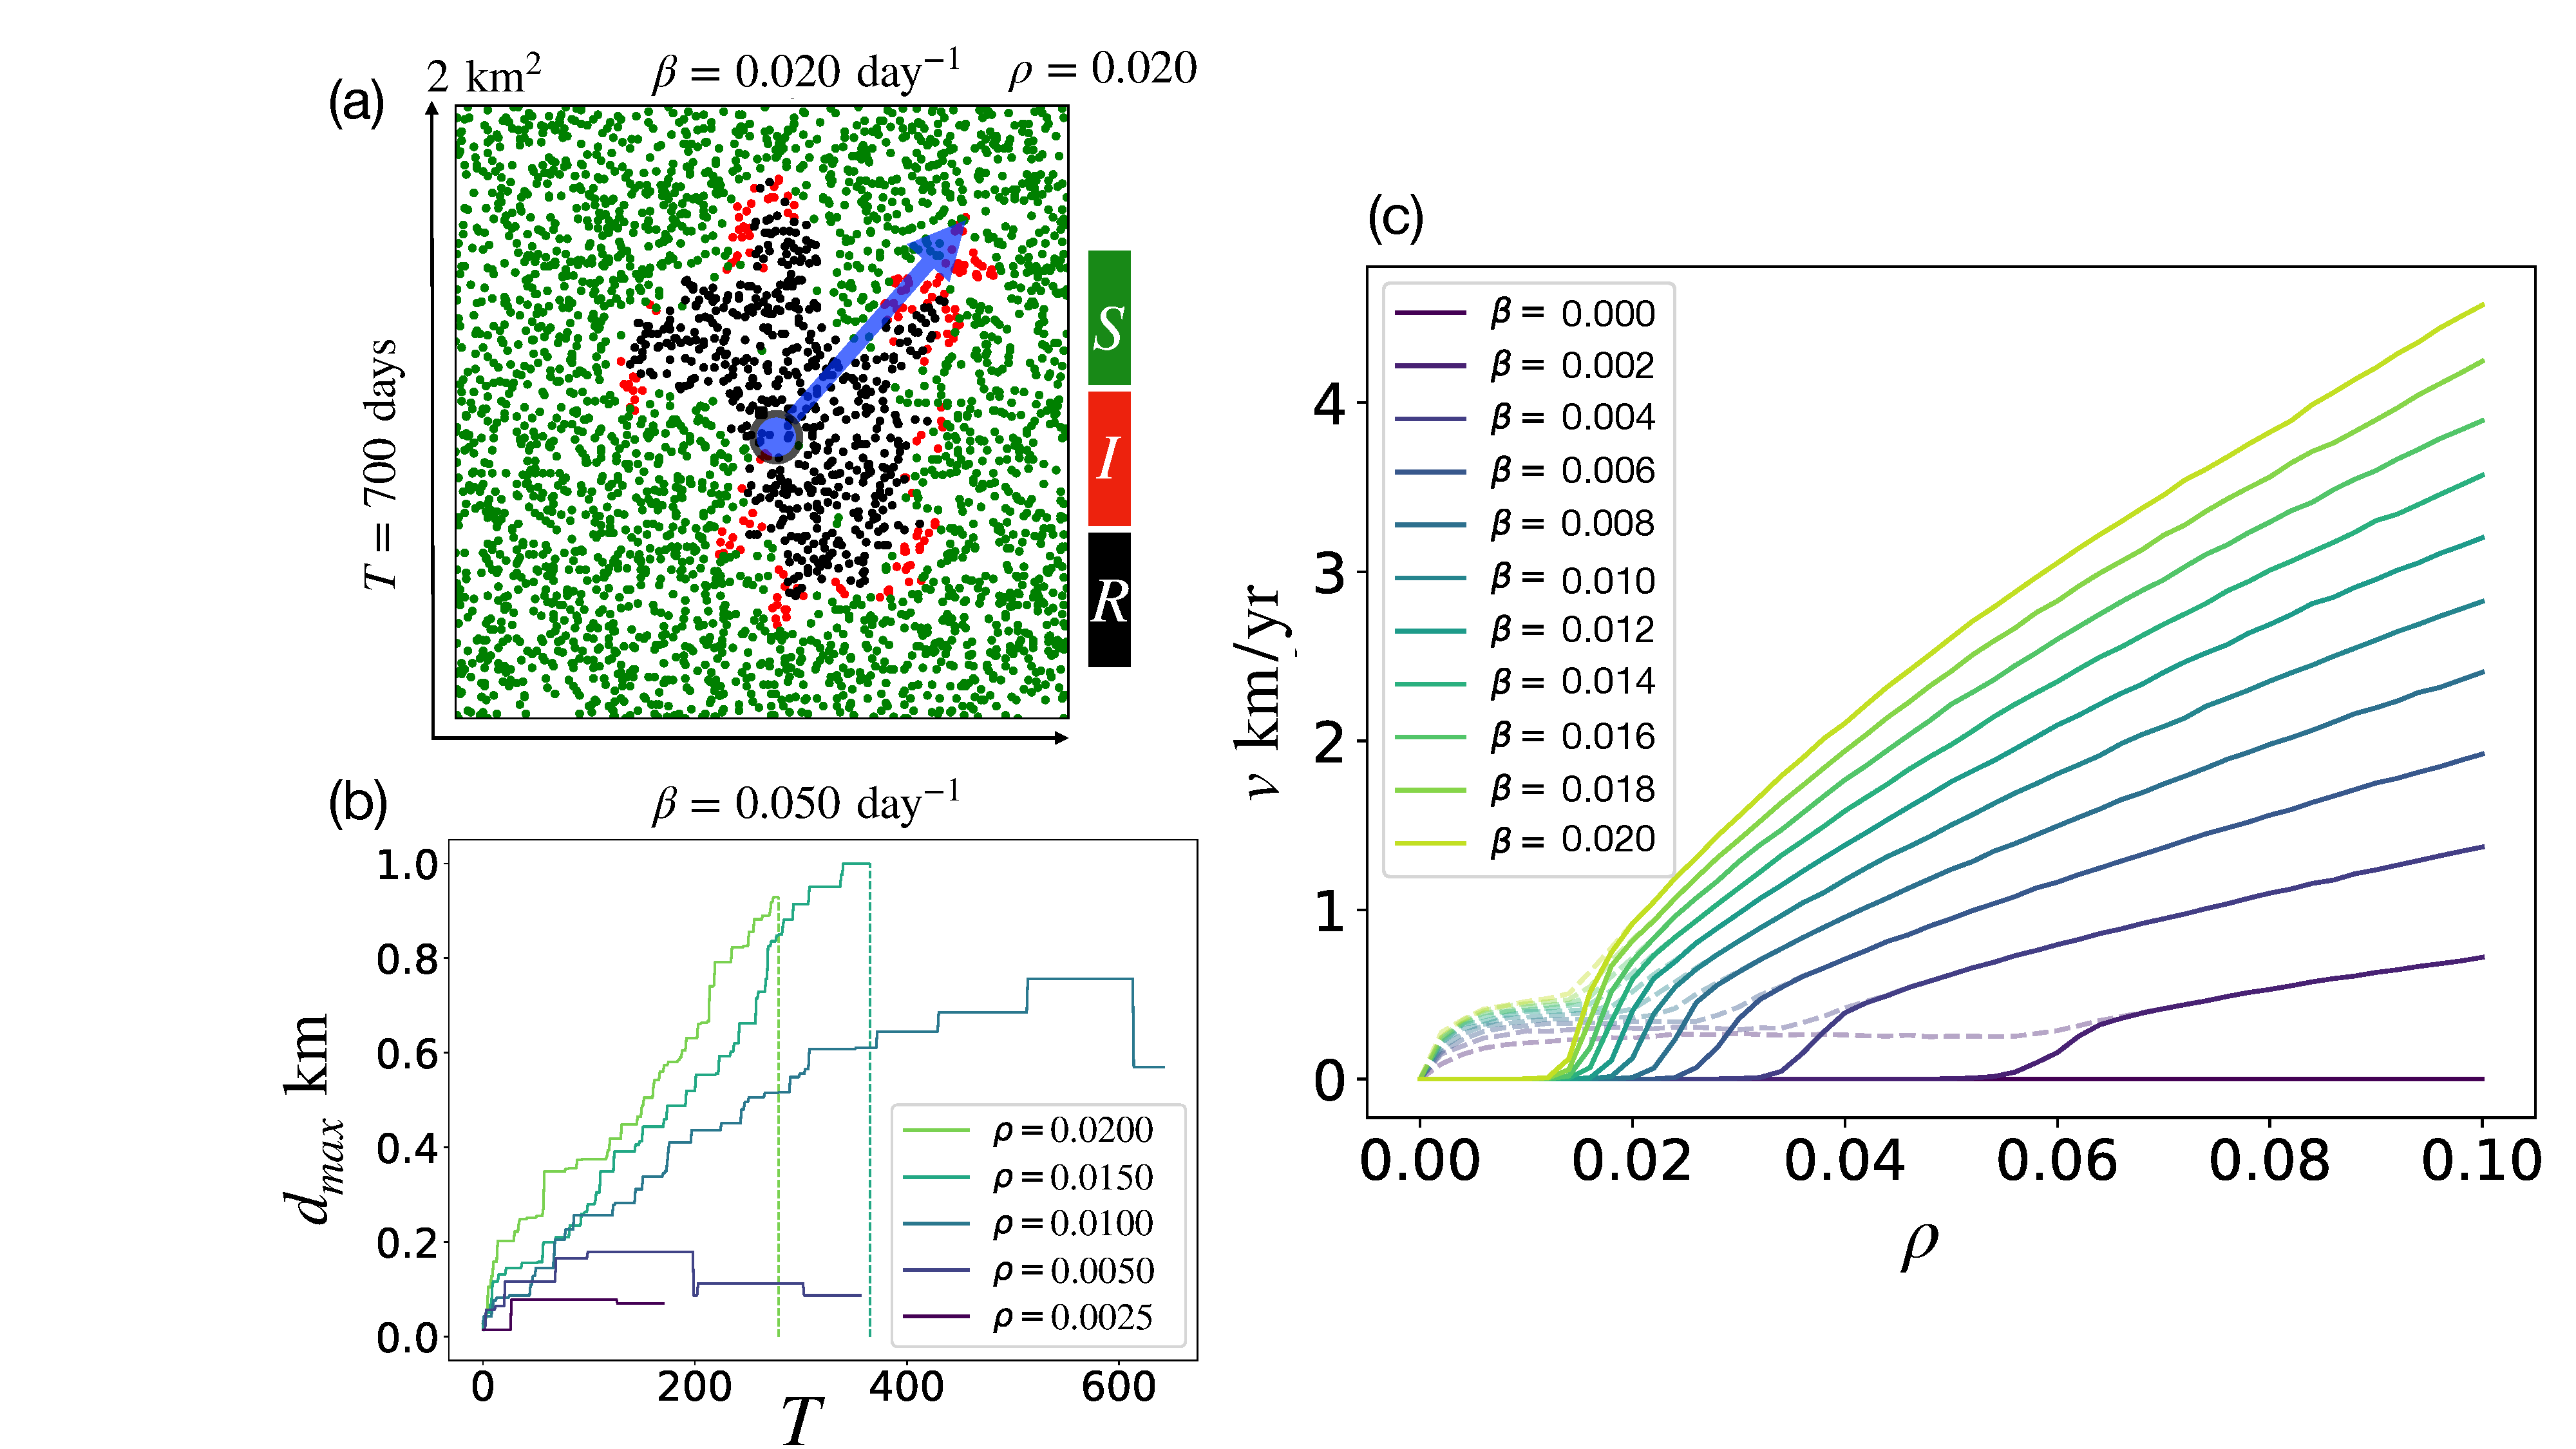
\includegraphics[scale=0.25]{chapter7/figures/figure3x.pdf}
    \caption{Generating estimates of the epidemic wave-speed from the non-local dispersal model, for fixed dispersal distance $\ell = 25\ \mathrm{m}$. (a) For each time-step in the dispersal model, a distance can be calculated by assessing the furthest position of an infected/removed tree away from the epicenter. (b) The time-series of maximum-distance is shown for fixed infectivity $\beta$ and five different parameter values of density $\rho$. An estimate for wave-speed is formed by dividing the maximum-distanced reached by the total elapsed time of the simulation. (c) Ensemble-averages of the wave-speed are shown for different combinations of $\rho$ and $\beta$.}
    \label{fig:fkpp-sgm-vel}
\end{figure}

\begin{figure}
    \centering
    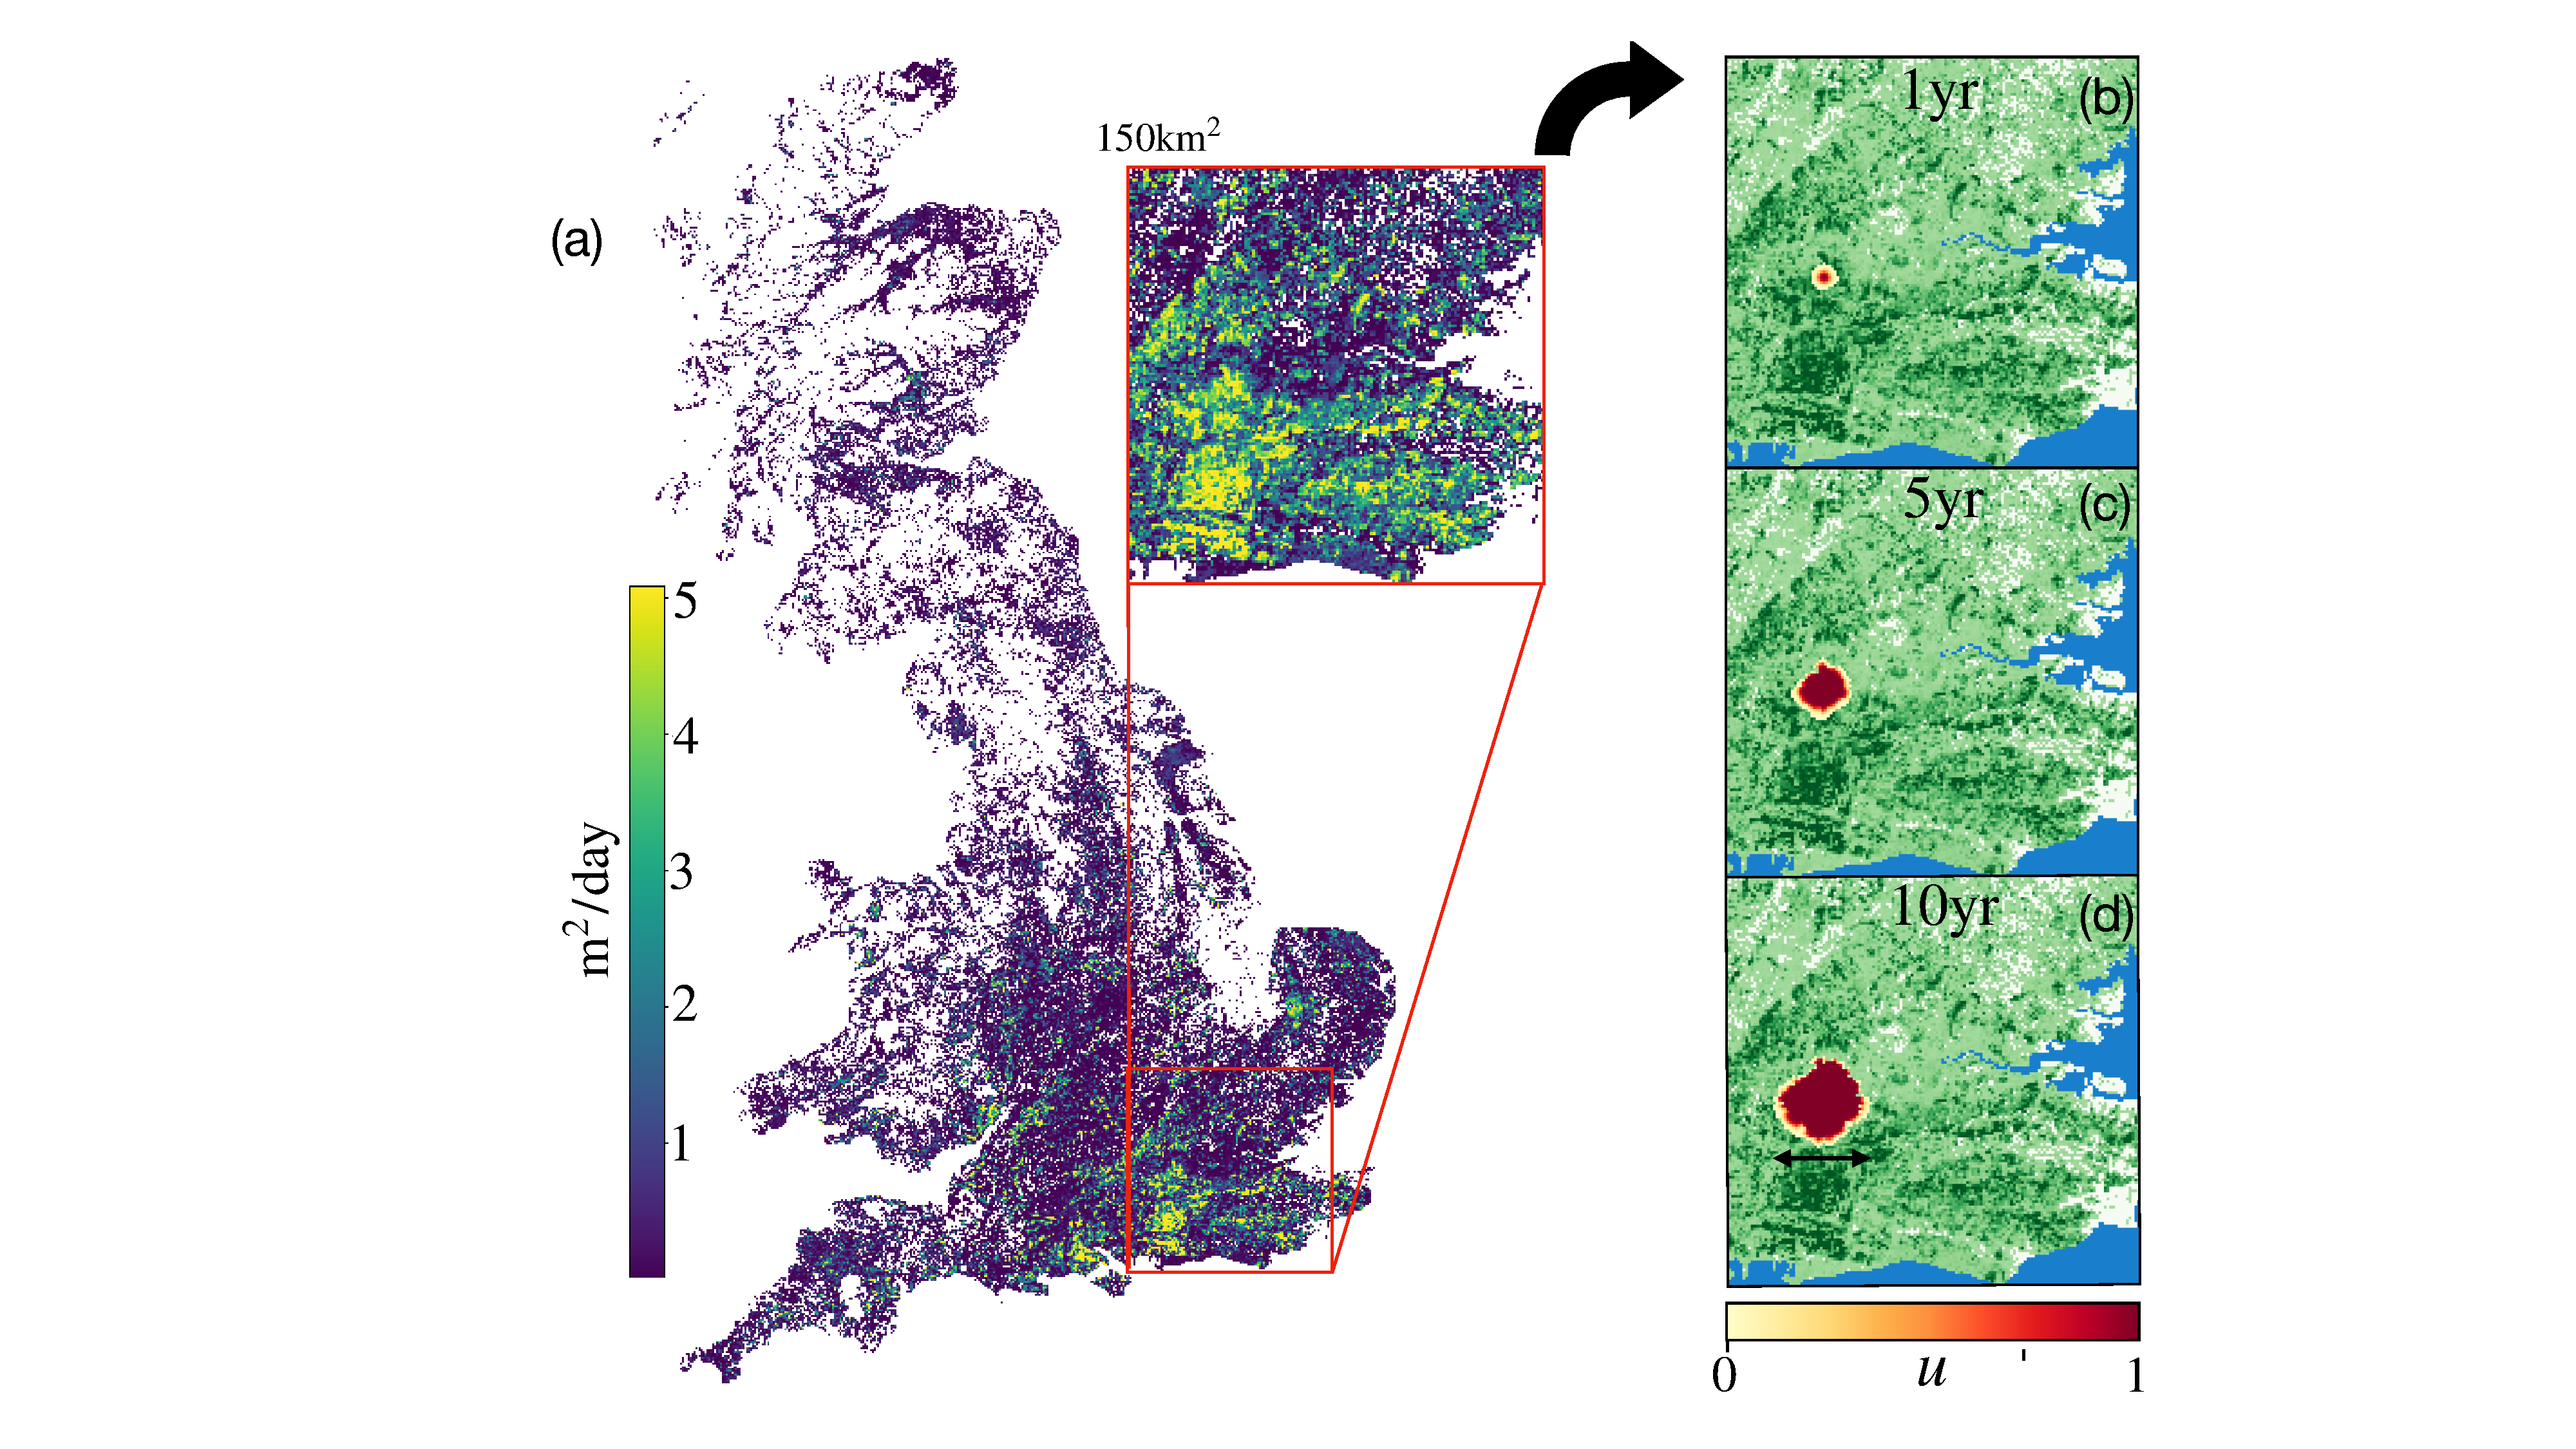
\includegraphics[scale=0.30]{chapter7/figures/figure4x.pdf}
    \caption{Diffusion coefficients generated from the sub-grid dispersal model for fixed parameters $r=0.01\ \mathrm{day^{-1}},\ \beta=0.020\ \mathrm{day^{-1}},\ \ell=25\ \mathrm{m}$. Diffusion value are projected onto the canopy cover data for Great British Ash distribution reported by \cite{hill.data}.}
    \label{fig:fkpp-diff}
\end{figure}

In the model,  constructed so far, there are three parameters that control the rate of spread: $\rho$, $\beta$ and $\ell$. %
Given that $\rho$ is fixed by the number of trees in the system, the only way to increase the speed of spread is to increase $\beta$ or $\ell$ (or both). %
However, as shown in Chapter \ref{chapter:regional-containment1} the relationship between $\beta$ and $\ell$ can be approximated to follow $\beta \propto \ell^{-2}$. %
Therefore, in order for the pathogen to spread faster the infectivity rate must substantially decrease in order to constrain realistic values of $R_0$. This precludes the possibility of increasing both $\beta$ and $\ell$ simultaneously. %

In order to avoid modelling unrealistic values of $R_0$ whilst increasing the rate of spread, %
we are left with the two options of increasing $\beta$ and decreasing $\ell$, or vice versa. %
Consider the thought experiment of increasing $\beta$ and decreasing $\ell$. Doing so would lead to more secondary infections inside a smaller area set by the dispersal kernel. %
On the other hand, if $\ell$ is increased and $\beta$ decreased, more secondary infections would result at further distances away from the infectious source. %
Thus, increasing $\ell$ and decreasing $\beta$ would at first appear to be means of constraining $R_0$ and increasing the speeds shown in Figure \ref{fig:fkpp-sgm-vel}(c). %
However, this in-turn leads to a problem which calls into question the validity of Gaussian dispersal. %


When $\ell$ becomes large in comparison to the average space between trees, %
a lower-rate of secondary infections amongst nearest-neighbours is observed in comparison to trees further away. %
This results because close to the source of infection, the  Gaussian dispersal does not decay rapidly enough. Pathogen dispersal with high values of $\ell$ can therefore become insensitive to immediate neighbours leading to a loss of short-range structure in the model. %
This exists in stark contrast to the intuitive notion that nearest-neighbours will become infected first, in response to an infected source. %
As discussed in Chapter \ref{chapter:regional-containment1} Gaussian dispersal was merely chosen as a convenient approximation. The limits of this approximation are now clearly exposed in the face of modelling longer-range dispersal events. %

%finish this please 
\section{Exponential dispersal}
%finish this please 
In Chapter \ref{chapter:regional-containment1}, the reproductive number $R_0$ of the model was explored in detail. Parameter values of $\beta=0.005\mathrm{day^{-1}}$ and $\ell\mathrm{m}$ were considered based on constraints of $R_0$, that is, roughly speaking $R_0 \in [0, 10]$. 
%finish this please 
\blindtext[1]
\blindtext[1]




\section{Chapter summary}
%finish this please 
\blindtext[1]
\textcolor{blue}{Detail all... the above...}






% 8) Final chapter

\chapter{Discussion}

In this thesis, a simple model of forest epidemics was incrementally extended into a more elaborate framework.
Each incremental improvement led to a novel, general-purpose framework to visualise epidemic severity across GB.
The framework is computationally efficient and adaptable to any wind-dispersed tree pathogen, provided a sufficient host density distribution is available. Conclusively, more research is required to progress and test the model against observational disease incidence data.
However, several exciting research avenues emerge from the work conducted in this thesis\textemdash discussed more below.

After setting the scene with a simple lattice model (SLM) of tree disease in Chapter \ref{chapter:SLM}, 
Chapter \ref{chapter:SLM-applications} linked the SLM with a map of predicted oak abundance given by \cite{hill.data} to produce a large-scale `toy' model. 
A key result emerged from Chapter \ref{chapter:SLM-applications}.
Namely, that \acrshort{nn} interactions were fundamentally insufficient to describe the spread of disease across lower, more realistic landscape tree densities. 
Fortunately, Chapter \ref{ch5:dispersal-model} resolved the issue by constructing a non-local dispersal model.
Nonetheless, Chapter \ref{ch5:dispersal-model} also demonstrated that a small dispersal length scale can still gives rise to an unnatural, wave/percolation-like epidemic. 
At the very least, these results bolster the growing body of research highlighting the importance of dispersal and help guide modellers to construct more representative models in botanical epidemiology.

Additionally, Chapter \ref{ch5:dispersal-model} examined two methods of calculating $R_0$ for a non-local dispersal model (NLM) over a range of epidemic parameters. Results from Chapter \ref{ch5:dispersal-model} indicate that when the scale of dispersal is comparable to the domain, the model approximates a mass-action well-mixed system described by the standard $SIR$ model. However, comparisons to the $SIR$ model were simplified and limited to one parameter (i.e. the ratio $\beta/\gamma$). Subsequently, the analysis constitutes a preliminary result, and a more sophisticated comparison method is required to glean further insight.

Most intriguingly, the spatially-explicit derivation of $R_0$ led to an `entire function' in Equation \ref{eq:ein}, a well-known function in complex analysis  \cite{abramowitz1948handbook}. 
Equation \ref{eq:ein} contrasts with the majority of approaches to calculate $R_0$, which generally rest on infectivity/removal rates without including spatial structure or dispersal. Instead, Equation \ref{eq:ein} was a function of infectivity, removal, dispersal, and tree density parameters. Further theoretical studies could explore a more rigorous analysis of Equation \ref{eq:ein}, and perhaps examine an alternate derivation incorporating inverse power law dispersal with exponentially-distributed removal lifetime dynamics.
However, it is clear to see that the mathematical derivation might ultimately become too challenging in the face of more complicated epidemic models. 

Then in Chapter \ref{ch5:dispersal-model}, the analytic expression of $R_0$ was compared against the `actual' contact-traced reproduction ratio. Both methods to determine the reproduction ratio demonstrated a clear epidemic threshold at $R_0=1$, thereby marking an important finding. Nevertheless, comparing both methods revealed that the analytic expression overestimates $R_0$ for progressively higher values ($R_0 \sim 10$), highlighting a significant limitation in the approach. 
Had the analytic expression been applied to a dense forest or highly aggregated distribution (where $\rho >10\%$ and $R_0$ is likely higher), the overestimation would only increase.
Therefore, the value of Equation \ref{eq:ein} rapidly diminishes when used to describe highly infectious regimes, but serves as an accurate approximation around the threshold $R_0 \approx 1$.

In contrast, the contact-tracing method computes the mean number of infections per infected tree over different infected generations.
Computing the mean-generational reproductive ratio proved convenient and led to a sharper epidemic threshold for later generations. These observations relate nicely to \cite{R0-perc-ref}, who studied a similar method to calculate $R_0$ for foot and mouth disease.
Despite the convenience of contact-tracing secondary infections in the model, it would be challenging to measure in natural systems experimentally.
As such, the method remains applicable to abstract modelling work alone and not in-the-field experiments.

The central value of Chapter \ref{ch:6-adb} results from outlining a novel framework to link a wind-dispersed epidemic model with species abundance data. 
The framework focused on the fungus ADB, which is well-established and already spread throughout Europe and the UK.
Thus, unfortunately, attempting eradication at this stage of pathogen development is untenable \cite{ash-dieback-costs}. 
Still, Chapter \ref{ch:6-adb} marks a step towards a general framework that can help policymakers reach informed decisions about \textit{where} to focus epidemic control.
In particular, the framework could provide value as an approach to threat assessment and rapid response modelling during the early phase of an epidemic.

In addition, Chapter \ref{ch:6-adb} developed a simplified spatially-explicit $SEIR$ model that described the seasonal spread of ash dieback (ADB) over local spatial scales.
Subsequently, the ADB model was coupled with the map of predicted ash abundance given by \cite{hill.data}, thus producing an $R_0$-map that covered GB.  
Surprisingly, no compartmentalised model of ADB could be found in the literature. Therefore, to my knowledge, the ADB model presented in this thesis 
is the first mechanistic (compartmentalised) attempt at modelling the epidemic spread of ADB.

Treating infectivity as a free parameter in Chapter \ref{ch:6-adb} led to several notable observations. When infectivity is low, the $R_0$-maps become sparsely populated with susceptible patches above the epidemic threshold. Consequently, the $R_0$-maps indicate that ADB would be unlikely to invade GB below a hypothetical minimum infectivity value.
In a similar vein, clusters in the $R_0$-map grew rapidly over four orders of magnitude between a narrow range of infectivity parameters.
Altogether, the model alludes to behaviour akin to a global epidemic phase transition across GB, though numerous assumptions place limitations on the framework.

As mentioned previously, infectivity ($\beta$) was unfitted to data and kept as a free parameter, enabling $R_0$-map analysis over a spectrum of infectivity parameters. 
However, arbitrarily defining infectivity underpinned a central limitation in work, and future research should aim to address this. 
Several works have published spatio-temporal and ADB mortality data in Europe \cite{https://doi.org/10.1111/1365-2745.13383, https://doi.org/10.1002/ppp3.11, stocks2017first, lohmus2014ash}, which could be used to estimate epidemic speed and lifecycle parameters using Bayesian Markov-chain-Monte-Carlo methods.
Similar approaches have been adopted to infer the spread of SOD in California \cite{10.1371/journal.pcbi.1002328} and citrus canker in Florida \cite{neri2014bayesian}, though no such work has been undertaken for ADB.
Further research is ultimately required to confirm the suitability of statistically fitting data to the spread of ADB, yet the prospect remains positive given the quantity of available data.

ADB mortality rates depend heavily on the landscape, composed of either rural, woodland or urban settings.
The type of environment is one particular consideration relevant for future epidemic parameter inference studies.
For simplicity, Chapter \ref{ch:6-adb} neglected environment types and employed a one-to-one mapping between infectivity and each $R_0$-map. In a more sophisticated model, each gird in the $R_0$-map would depend on a $\beta$ parameter dependent on the type of environment.
Thus, statistical inference based on the environment type goes hand-in-hand with improving accuracy in the $R_0$-map.
The national forest inventory could conveniently aid these future improvements, as it holds relevant information on which regions are woodland, forest or urban\textemdash discussed previously in section \ref{sec:nationa-surveyes}.

Chapter \ref{ch7:landscape-level-control} outlined the first steps toward epidemic control predicated on the host spatial structure.
That is, identifying and targeting positions in the host distribution that may disrupt epidemic dispersal between regions.
Initial results reveal that epidemic connectivity can depend on a small number of `connecting' positions in the host distribution.
Nevertheless, more research is required to assess the utility and efficiency of the control strategy. Chapter \ref{ch7:landscape-level-control}
outlined a potential research direction to examine and test the control strategy by considering a set of coupled patches in section \ref{sec:future-questions}.
From the coupled system,  the transmission probability and effect of control between host patches can be assessed.
Until this work is undertaken, the strategy remains speculative.
Following the research direction posed in section \ref{sec:future-questions}, future work should develop the definition of connectivity inside the $R_0$-map. Each pixel within an $R_0$-map reflects only isolated within-patch interactions and not between-patch LDD.
As such, there is no non-local connectivity between pixels in the map, 
a limitation clearly revealed when analysing clusters at different landscape resolutions in section \ref{sec:gaussian-r0-clustering}.

Unsurprisingly, insufficient host data underpins a significant limitation in this thesis.
Although the predicted ash abundance map captured the overarching large-scale distribution of ash in GB, Hill et al. reported a RMSE of $5\mathrm{ha}$. Therefore, in reality, regions below the threshold might be susceptible\textemdash and vice-versa for above threshold regions.
Unfortunately, such errors mean that the host distribution is not accurate enough to inform the hypothetical (fine-scale) management scenarios presented in Chapter 7. Until species abundance data captures the host distribution more reliably, country-wide applications remain extraordinarily ambitious. In response to this limitation, future research could concentrate on smaller-scale areas where abundance data is known. For example, by examining well-surveyed areas inside the UKCEH Countryside Survey data.

In conclusion, the research narrative developed in this thesis aims to help inform policymakers about where to focus epidemic control.
The approach constitutes an epidemic mapping framework for tree disease with parallels to the emerging field of Infectious Disease Cartography in human epidemiology. 
The framework is computationally efficient, flexible, and adaptable to other pathosystems.
Several theoretical insights were ascertained from deriving a spatially-explicit expression for $R_0$ and comparing it against a stochastic non-local dispersal model. Lastly, a novel epidemic control strategy was outlined, though more work is needed to progress the framework and rigorously validate results.

% The framework produced epidemic maps  differs from other large-scale approaches to model the spread of tree disease 
% Infectious Disease Cartography, one seeks to map the likelihood, or risk, of infectious disease outbreaks and produce risk-maps.
% Infectious Disease Cartography
% Disease cartography using 

% \begin{itemize
%     \item We have...Disease cartography using liking species abundance with spatially-explicit epidemic model. A notable challenge posed by a dispersal-based system
%     is that regions of land couple together non-locally. Throughout this thesis, CCA assessed clustering based on neighbour links. 
%     Going forward, a more sophisticated notion of connectivity could permit higher resolution maps for Inverse power law... method could add significant value... 
%     \item focus on a small study area, as in \cite{he2019integrating}
% \end{itemize}

%---------------------------------------------------------
% relation of work to more commonplace Metapopulation models
% In the process of computing a value for $R_0$, several insights into dispersal-based epidemic progression and spatial-scale came to light.
% Namely, computing $R_0$ for a fat-tailed inverse power law dispersal kernel required a larger to domain-size in comparison to the thin-tailed Gaussian variants.
% A larger domain-size necessitated a lower landscape-level resolution (or equivalently larger patch-size) when forming the $R_0$-map.
% Thus to define an $R_0$-value in the framework, landscape-level patch-size needs to reflect the nature of dispersal;
% metapopulation-type models do not have this limitation. 
% Yet, at the same time typical metapopulation models are not predicated on small-scale epidemiological properties, 
% but tend to model patch-sizes on the order of $100\mathrm{m}-1\mathrm{km}$ \cite{large-scale-control, doi:10.1111/j.1365-3059.2010.02391.x}.

%---------------------------------------------------------
% generalisation to the approach
% In favour of parsimony, infectivity $\beta$ was kept constant over the entire landscape of Great Britain.
% However, epidemic severity of ADB is known to vary in response to either urban or rural environments \cite{marciulyniene2017can}.
% So in reality, $\beta$ may very well exhibit a spatial dependence.
% Likewise, including an index on, $\beta_i$, could reflect yearly changes due to climate change or habitat suitability\textemdash thus generalising the yearly infection cycles according to Figure \ref{fig:SEIR-transitions}.
% An attractive feature of the $SEIR$ model therefore includes the scope of its adaptability 
% and generalisations to our notion of $\beta$ could support more in-depth studies on spatio-temporal epidemic heterogeneity.

%-------------------------------------------------------
% - Crucially, future work will involve integrating LDD mechanisms into the model in order to understand the relative importance long vs local distance dispersal. We may speculate about the relative importance looking at figure x, whereby the maximum distance spread in season due to local-scale spread is xm/year, in stark contrast from the observed spread of 40-60km/yr.
% - We cannot overstate the importance of LDD, and it is hard to say the degree to which targeting the local dispersal mechanism alone will inhibit the spread. We will revisit this question in future work, however, we contend that preferentially targeting diseased trees based on spatial location.....could help control epidemics with greater efficacy. 
% - We may speculate how our result could aid the effort of choosing where to re-plant ash stands genetically engineered to be less susceptible; if re-planting efforts were undertaken in certain location.... <- speculative
% - We may speculate about how persistent ash dieback would be, even if a large-scale control effort was undertaken
% - There is evidence to suggest regional variation in mortality due to ash dieback \cite{stocks2017first}, this could be incorporated into the model...
% - Recently, it has been suggested that the dispersal-kernel of wind-borne pathogens might follow a scaling law \cite{https://doi.org/10.1111/jbi.13642}


\appendix
\chapter{Simple lattice Model}

\section{Propagation algorithm}
\label{a:propagation}
Starting from simplicity, the model assumes local transmission between nearest neighbours. Local structure within the network is described by the von Neumann neighbourhood. To demonstrate the algorithm, take a $3 \times 3$  matrix $\mathbb{S}$ representing a small patch of forest, $1's$ represent trees in state $S$ while $0's$ represent insusceptible states $\emptyset$. An and infection matrix $\mathbb{I}$ is defined with an infected matrix element $I_{2,2}=2$. A removed matrix is also given by $\mathbb{R}$. At time $t=0$:
\begin{equation}
\mathbb{S}= \left( \begin{array}{ccc}
0 & 1 & 0\\
1 & 0 & 0\\
0& 1 & 0 \\
\end{array} \right)\qquad
\mathbb{I}= \left( \begin{array}{ccc}
0 & 0 & 0\\
0 &2 & 0\\
0& 0 & 0 \\
\end{array} \right)\qquad
\mathbb{R} = \left( \begin{array}{ccc}
0 & 0 & 0\\
0 & 0 & 0\\
0 & 0 & 0 \\
\end{array} \right)\qquad
\end{equation}

\subsection{Assessing the probability of transition}
\label{a:probablity-transition}

A centrally infected state in $\mathbb{I}$ can be seen\textemdash when $\mathbb{I}_{i,j} = 2,\ \mathbb{S}_{i,j} = 0$. The algorithm singles out neighbours surrounding the infected tree and generates random numbers $\{ R_{0,1},R_{1,0},R_{3,2}\}$. From this a potential infection matrix $\mathbb{I}^{'}$ is formed:

\begin{equation}
    \mathbb{I}^{'} = \begin{pmatrix}
        0 & R_{0,1} & 0 \\
        R_{1,0} & 2 & 0 \\
        0 & R_{2,1} & 0 
     \end{pmatrix}
\end{equation}

Each random number is generated uniformly between $[0,1] $. If  $R_{i,j} \leqslant \beta$ the infection jumps to site $(i,j)$. For example, assume $R_{0,1}\leqslant \beta$ and $R_{1,0}, R_{2,1} \geq \beta $, then at time $t=1$ the matrices are updated:

\begin{equation}
    \mathbb{S} = \left( \begin{array}{ccc}
    0 & 0 & 0\\
    1 & 0 & 0\\
    0& 1 & 0 \\
    \end{array} \right)\qquad
    \mathbb{I}= \left( \begin{array}{ccc}
    0 & 2 & 0\\
    0 & 3 & 0\\
    0& 0 & 0 \\
    \end{array} \right)\qquad
    \mathbb{R}= \left( \begin{array}{ccc}
    0 & 0 & 0\\
    0 & 0 & 0\\
    0 & 0 & 0\\
    \end{array} \right)\qquad
\end{equation}
    
When $\mathbb{I}_{i,j}=T+1, \mathbb{R}_{i,j} = 1$. The algorithm is repeated over a set time-horizon (typically $t=3000$) and eventually one of the three boundary conditions is met and the simulation ends. In python this is implemented by matrix operations:

\begin{lstlisting}[style=pythoncode,
    caption = An alorithm written in python to compute matrix equations and simulate disease spread. Code can be found in: \textcolor{red}{cite github repo?}.,
    label = py:rand]

def run(S, I, R, beta, T=10, L=500):
    """
    Run algorithm
    :param S: array-like, susceptible matrix
    :param I: array-like, infected matrix
    :param R: array-like, removed matrix
    :param beta: float, transmission probability
    :param T: int, infectious life-time of a tree
    :param L: int, lattice dimension
    :return:
    """
    # - Begin - #
    for t in range(3000):
            # nn : nearest neighbours, 
            # - single out vertical and horizontal nn respectively
            nn = np.roll(I, 1, axis=0) + np.roll(I, -1, axis=0)
            nn = nn + np.roll(I, 1, axis=1) + np.roll(I, -1, axis=1)
            nn = (nn * S) > 0  # sigle out susceptible trees only
            # inf_dyn : infection dynamics (a probability)
            inf_dyn = np.array(np.random.uniform(size=[L, L]) < beta)
            # add 1 to exitsting ifectes 
            # combine neaibourhood to infection status
            I = I + (I > 0) + 2 * nn * inf_dyn. 
            S = S * np.where(I > 0, 0, 1) # take away infecteds from S
            R = R + np.where(I == T, 1, 0)  # transition I to R
            R = np.array(R_tree > 0).astype(int). # Hold R as binary
            I = I * np.where(R > 0, 0, 1) # Remove infected status 
            # continue...
\end{lstlisting}


\section{Towards a continuum model}
\label{a:slm-mean-field-theory}

% section short summary:
Here, we move away from the discrete stochastic percolation model outlined previously and examine alternate modelling paradigms. 
A set of field equations describing the evolution of the probability fields $S$, $I$ and $R$ for the simple lattice model are described.

From the percolation model in section \ref{ch3:two-param-model}, three states were defined for each lattice site $i$: susceptible, infected, removed $S_i, I_i, R_i$. The evolution of these lattice sites were dictated by Mote-Carlo steps where each infected lattice site has a chance to infect a nearest neighbour moving a susceptible tree in state $S$ to infectious state $I$ before finally transitioning into the $R$ compartment in $T=10$ time steps. Each simulation can be seen as an individual realisation of the physical process, however, a great many other potential realisations could have occurred. This is easily demonstrated around percolation threshold where successive iterations lead to differing results, some simulations will percolate and be considered an epidemic while some will not. Even if well above or below the threshold of transmission, infected trees will propagate differently and trace out unique pathways through the domain owing to a very small probability of tracing out exactly the same pathway. Therefore, this individuum paradigm is noisy and only useful for understanding average behavioural quantities when ensemble averaged which is limited in scope by computer memory.

An alternate method, requiring no ensemble-averaging, would be to formulate a set of differential equations which describe the probability-evolution of lattice sites $i$ in the domain being in either states $S,I,R$. This method would yield the benefit of not needing to ensemble-average results in order to determine average behaviours as a single iteration of the simulation by construction gives us the \textit{mean} field evolution. Furthermore, simulations when animated spatially would give \textit{average} travelling wave behaviour equivalent to running many stochastic simulations and combining frames (which could require large amounts of data). As before, the initial population of trees in the domain is seeded with probability $p$, with exception of a small number of initially infected trees at the center of the domain. The empty lattice sites at $t=0$ and the removed lattice sites at $t \ge T$ behave exactly the same remaining non-infectious to susceptible trees therefore both empty and removed lattice sites can be described by state $R$
\begin{equation}
       S_i = p;\quad I_i = 0;\quad R_i = (1 - p) 
\end{equation}{}

Where $p$ is the probability of being occupied by a susceptible tree (\textit{equivalent to tree density}). Now a set of dynamical equations which govern the evolution of fields $S,I,R$ can be outlined by considering the dynamics of the simple lattice model; over a single time-step an infected tree at position $i$ has probability $\beta$ of infecting a healthy nearest neighbour, this is given by $\beta I(t)_i$ i.e. the probability of transmission multiplied by the probability being infected. Considering a healthy tree at position $i$ surrounded by 4 nearest neighbours $j$, where j denotes $j= \pm \Delta x $ or $ j=\pm \Delta y$, we can describe the probability of $S_i$ remaining healthy by: 
\begin{equation}
    \prod_j (1 - \beta I(t)_{i+j})
    \label{eq:rep-prod-S}
\end{equation}{}
where the repeated product gives us the chance of \textit{not being} infected iterated over all nearest neighbours \footnote{In reality the event of a healthy tree being infected by its neighbours are statistically independent events and therefore calculating the total probability of being infected constitutes a combinatorics problem of combining the union of n events. It is much simpler to consider the single event of \textit{remaining healthy}.}. The reduction of probability in a tree at site $i$ remaining susceptible is then given by:
\begin{equation}
    S_i(t+\Delta t) - S_i(t) =  - S_i(t)\prod_j \Big [1 - \beta I(t)_{i+j} \Big ] 
    \label{eq:s-field-evol}
\end{equation}{}
From this, the field $S$ can be seen to monotonically decrease. From this point it is easiest to consider the evolution of field $R$. In the simple percolation model transition times where set to $n$ time-steps before an infected tree transitions into the removed compartment, therefore a tree infected at time-step $t-n\Delta t$ will during time-step $t \rightarrow t + \Delta t$. In original simulations in chapter \ref{ch3:two-param-model} the value was held constant at $n = 10$. The change in field $R$ can then be given in terms of field $S$ by:
\begin{multline}
     R_i(t+\Delta t) - R_i(t)  = -\Big[S_i(t - n\Delta t) - S_i(t-(n+1)\Delta t\Big] = \\
     S(t - (n+1)\Delta t) \Big[ 1 - \prod_j \big(1 - \beta I_{i+j}(t - (n+1)\Delta t)\big)\Big]
     \label{eq:r-field-evol}
\end{multline}
Where the right hand side of the top line is substituted with the right hand side of equation \ref{eq:s-field-evol} at time $t-(n+1)\Delta t$. Lastly, noting that all probabilities add to unity, $S_i(t) + I_i(t) + R_i(t) = 1$, the equations which govern the evolution of infectious field $I$ can be written as:
\begin{multline}
    I_i(t+\Delta t) - I_i(t) = S_i(t)\Big[1 - \prod_j\big( 1 - \beta I_{i+j}\big)\Big] - \\ S(t - (n+1)\Delta t) \Big[ 1 - \prod_j \big(1 - \beta I_{i+j}(t - (n+1)\Delta t)\big)\Big]
    \label{eq:i-field-evol}
\end{multline}

equations \ref{eq:s-field-evol} - \ref{eq:i-field-evol} are finite-difference equations and thus describe the evolution of probabilities at lattice site $i$ given a set of initial conditions. These finite difference equations can be iterated over a set of time-steps to model average behaviour of an ideal system away from the critical regime. At criticallity there will be large fluctuations in behaviour, as the system is in a highly chaotic state and does not belong to any one power-law distribution, therefore simulations would deviate quite considerably and fail to show any fractal-like critical structure. Furthermore, equations \ref{eq:s-field-evol} - \ref{eq:i-field-evol} only describe systems of sufficiently large domain size due to domain sensitivity effects.

\begin{figure}
    \centering
    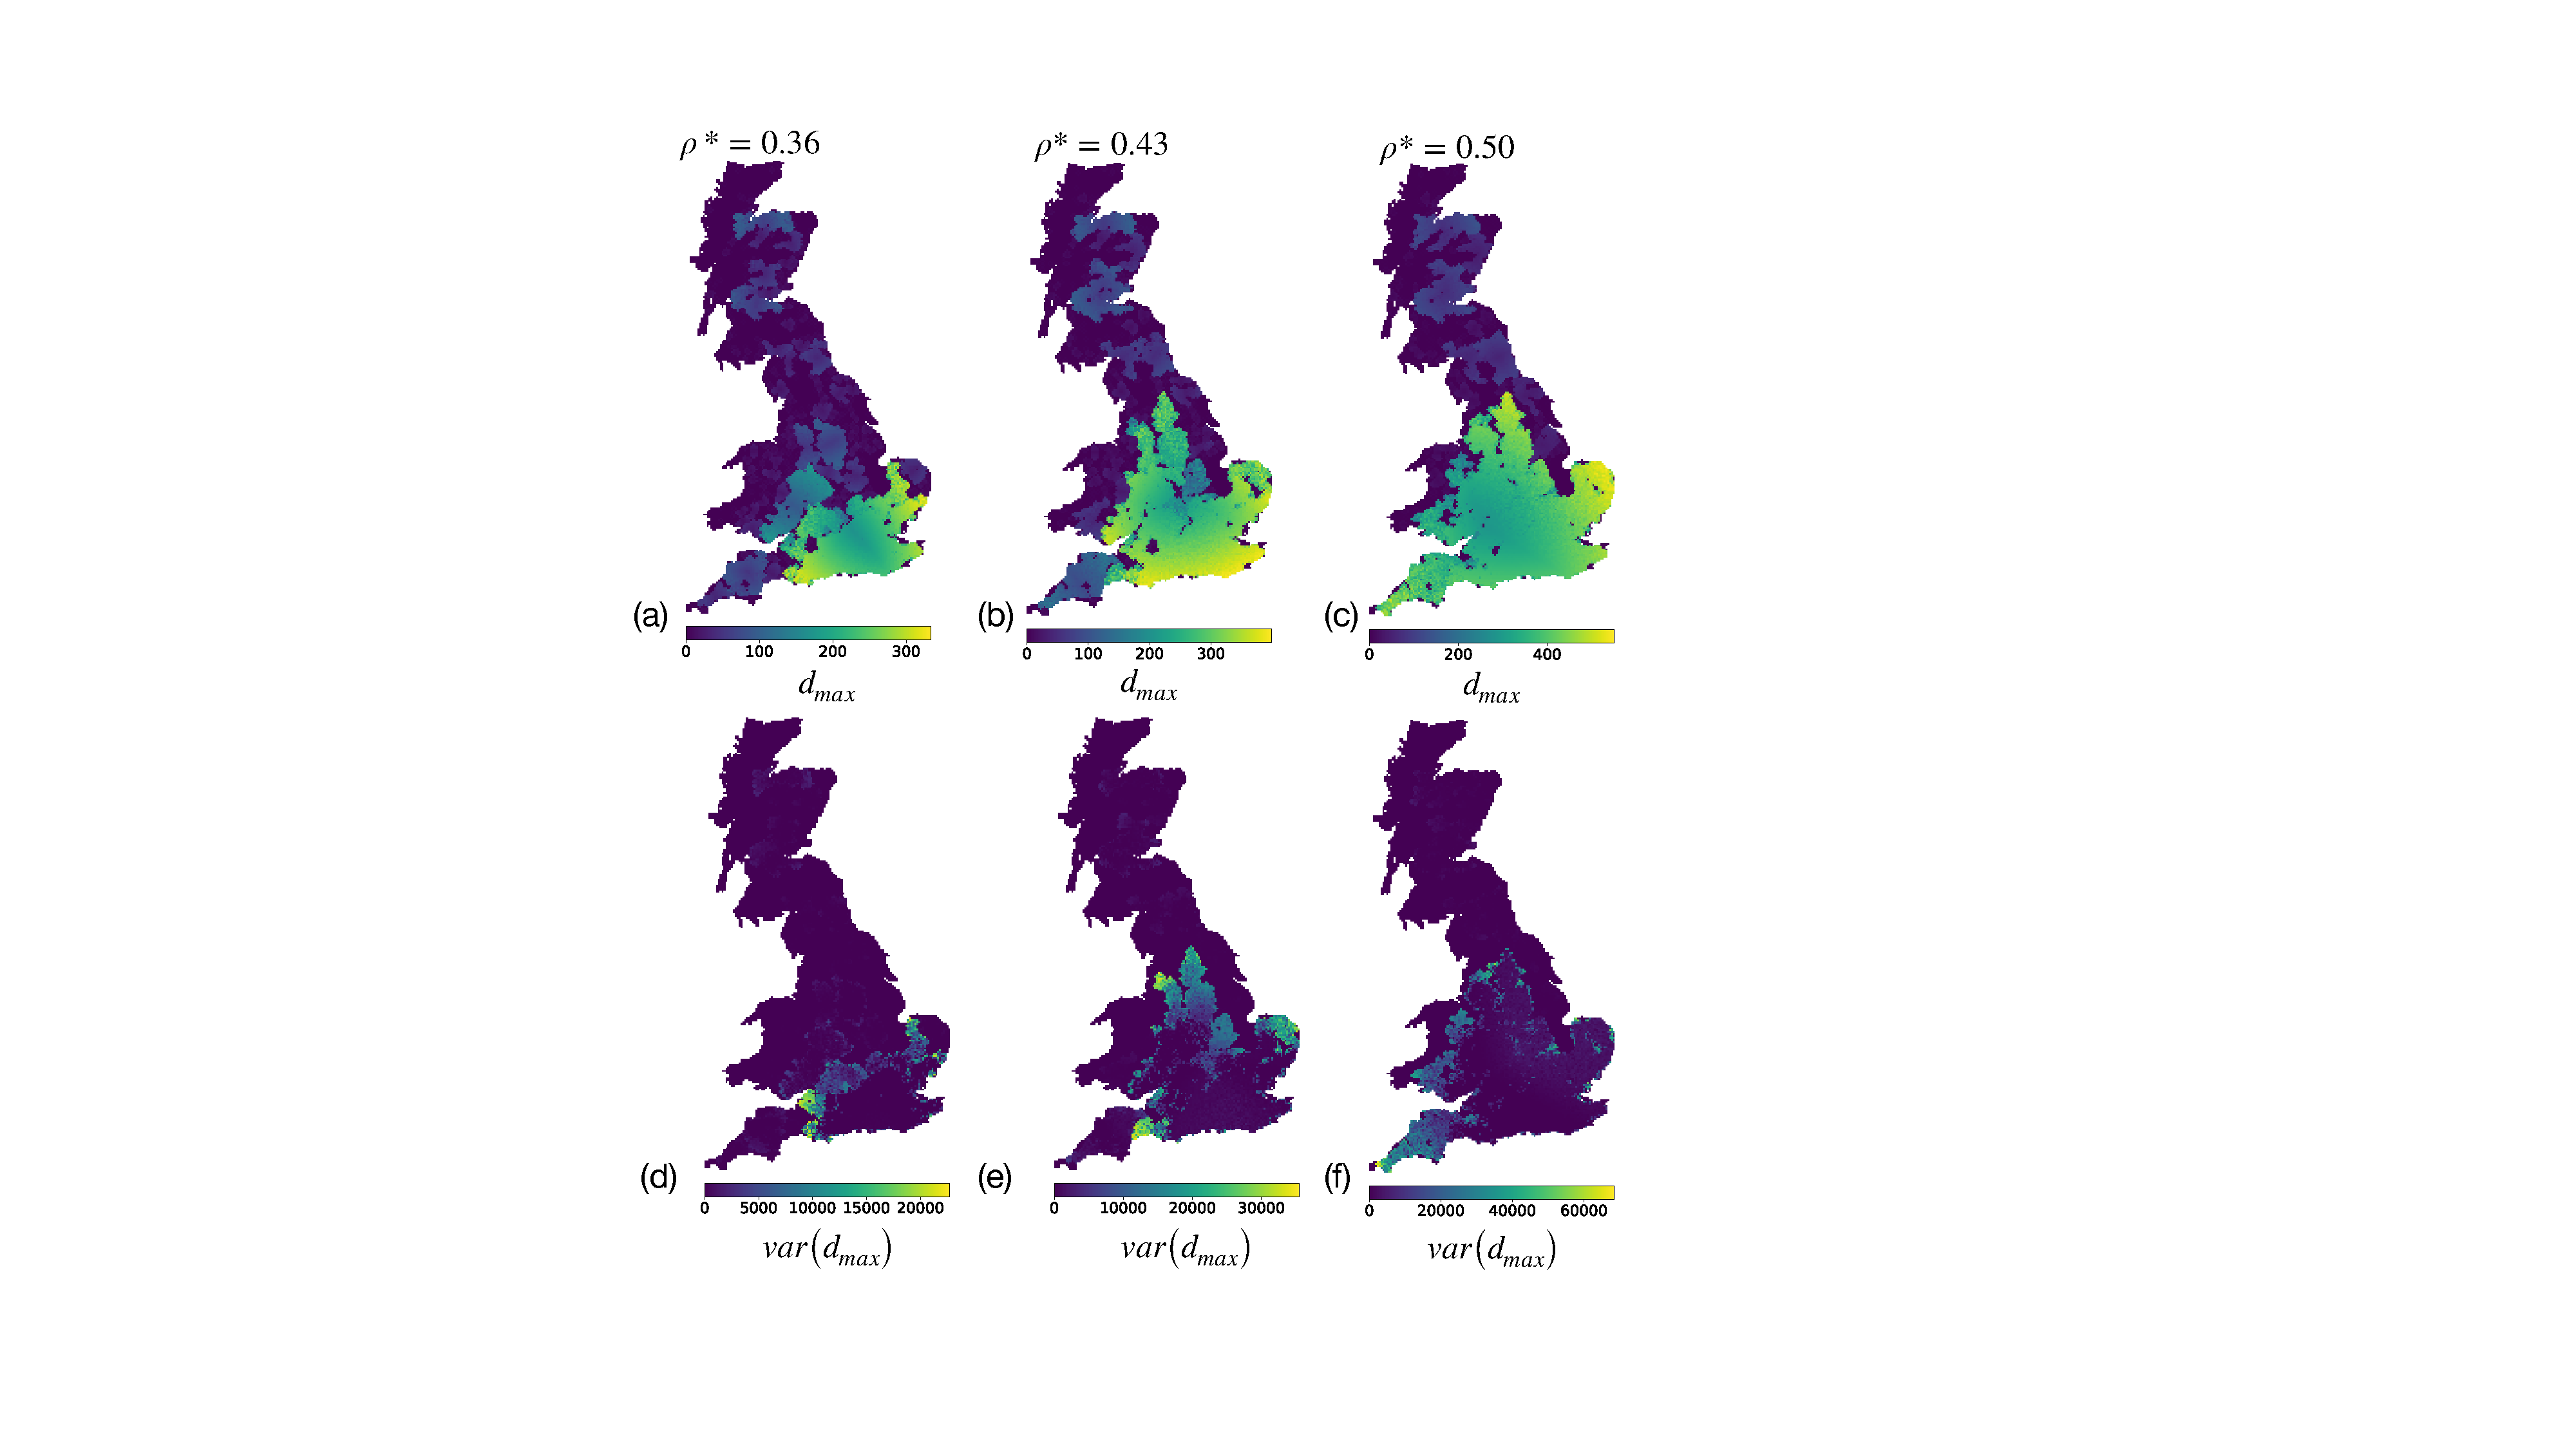
\includegraphics[scale=0.55]{appendix/figures/A-ch4figure1.pdf}
    \caption{The max-distance ($d_{max}$)} metric...
    \label{fig:my_label}
\end{figure}

\chapter{The non-local dispersal model}
\label{section:apendix_A}

\section{An alternate derivation}
\label{eq:alternate-R0}
Starting from an un-normalised Gaussian kernel $g(p, q; \ell) = \exp(\frac{p^2-q^2}{2\ell^2})$ and infectivity constant $\beta$, we may define the probability of position $q$ being infected due to an infected tree at $p$ as $Pr(q; p) = \beta g(p, q; \ell)$. The domain has tree density $\rho_0$ at time $t=0$ and trees transition through states: $S\rightarrow I\rightarrow R$, with $I$ lasting for $T$ time-steps. Considering the probability of point $q = (x, y)$ becoming infected on account of an infected tree located at the origin during the first time-step:
\begin{equation}
    Pr(x, y, t=0) = \beta \rho_0 \exp(-\frac{x^2+y^2}{2\ell^2})
\end{equation}{}
 Integrating this over an infinite domain gives $R_0(t=0)$ expected infections, given by:
\begin{equation}
    R_0(t = 0) = \beta \rho_0 \int^{\infty}_{-\infty} \exp(-\frac{x^2+y^2}{2\ell^2})dx dy= 2\pi\beta\rho_0\ell^2
\end{equation}{}
At time-step $t+1$ there are less trees to infect. Therefore tree density $\rho$ should also be considered as a monotonically decreasing function of time $\rho(t)$, and the number of expected infections should be given by:
\begin{equation}
    R_0(t) = 2\pi\beta\ell^2\rho(t)
    \label{eq:r0-A}
\end{equation}{}
 Considering density as a function of time\footnote{Density also varies with space as trees are removed quicker for regions closer around the primary infection. However, negating this lead to an easily solvable expression valid for lower-value regimes.} in a discrete domain of size $L$, the average decrease in tree density over one time-step is given by:

\begin{equation}
\label{eq:discrete-rho-t-A}
\begin{split}
\rho(t+1) & = \rho(t) - \frac{R_0(t)}{L^2} \\
 & = \rho(t)\Big(1 - 2\pi\beta\frac{\ell^2}{L^2} \Big)
\end{split}
\end{equation}

at $\rho(t=0)=\rho_0$, therefore, equation (\ref{eq:discrete-rho-t-A}) forms a series from which we may expand to give a continuous equation of $\rho$:
\begin{equation}
    \rho(t) = \rho_0 \big(1 - 2\pi\beta\frac{\ell^2}{L^2}\big)^t
\end{equation}{}
upon substitution back into equation (\ref{eq:r0-A}) we have an approximation for how the number of expected infections from one infected tree is expected to change over time:
\begin{equation}
    R_0(t) = 2\pi\beta\ell^2\rho_0 \big(1 - 2\pi\beta\frac{\ell^2}{L^2} \big)^t
    \label{eq:Rt-A}
\end{equation}{}
This expression is compared against numerical simulations in Fig \ref{fig:sgm-evol}(c). Then integrating over the infectious life-time $t=T$ gives an approximation to an effective reproductive number denoted by $R_0$:

\begin{equation} \label{eq1}
\begin{split}
R_0 & = 2\pi\beta\ell^2\rho_0 \int ^T _0 \big(1 - 2\pi\beta\frac{\ell^2}{L^2} \big)^t dt \\
 & = 2\pi\beta\ell^2\rho_0 \frac{ (1 - 2\pi \beta\frac{\ell^2}{L^2})^T - 1}{\ln(1 - 2\pi\beta\frac{\ell^2}{L^2})}
\end{split}
\end{equation}

(from $\int c^t dt = \frac{c^t}{\ln(c)}$). The expression for $R_0$ can be simplified by noting the pathogen is unlikely to infect trees beyond a distance of $3\ell$, therefore, we can replace the area of the domain with the area over three standard deviations (i.e. $9\pi\ell^2$), thus leading to the approximation:
\begin{align*}
    R_0 = 2\pi\beta\rho_0\ell^2 \frac{(1 - 2/9\beta)^T - 1}{\ln(1-2/9\beta)}
\end{align*}

\newpage

\section{SIR fitting}
\label{A:sir-fitting}
\begin{figure}
    \centering
    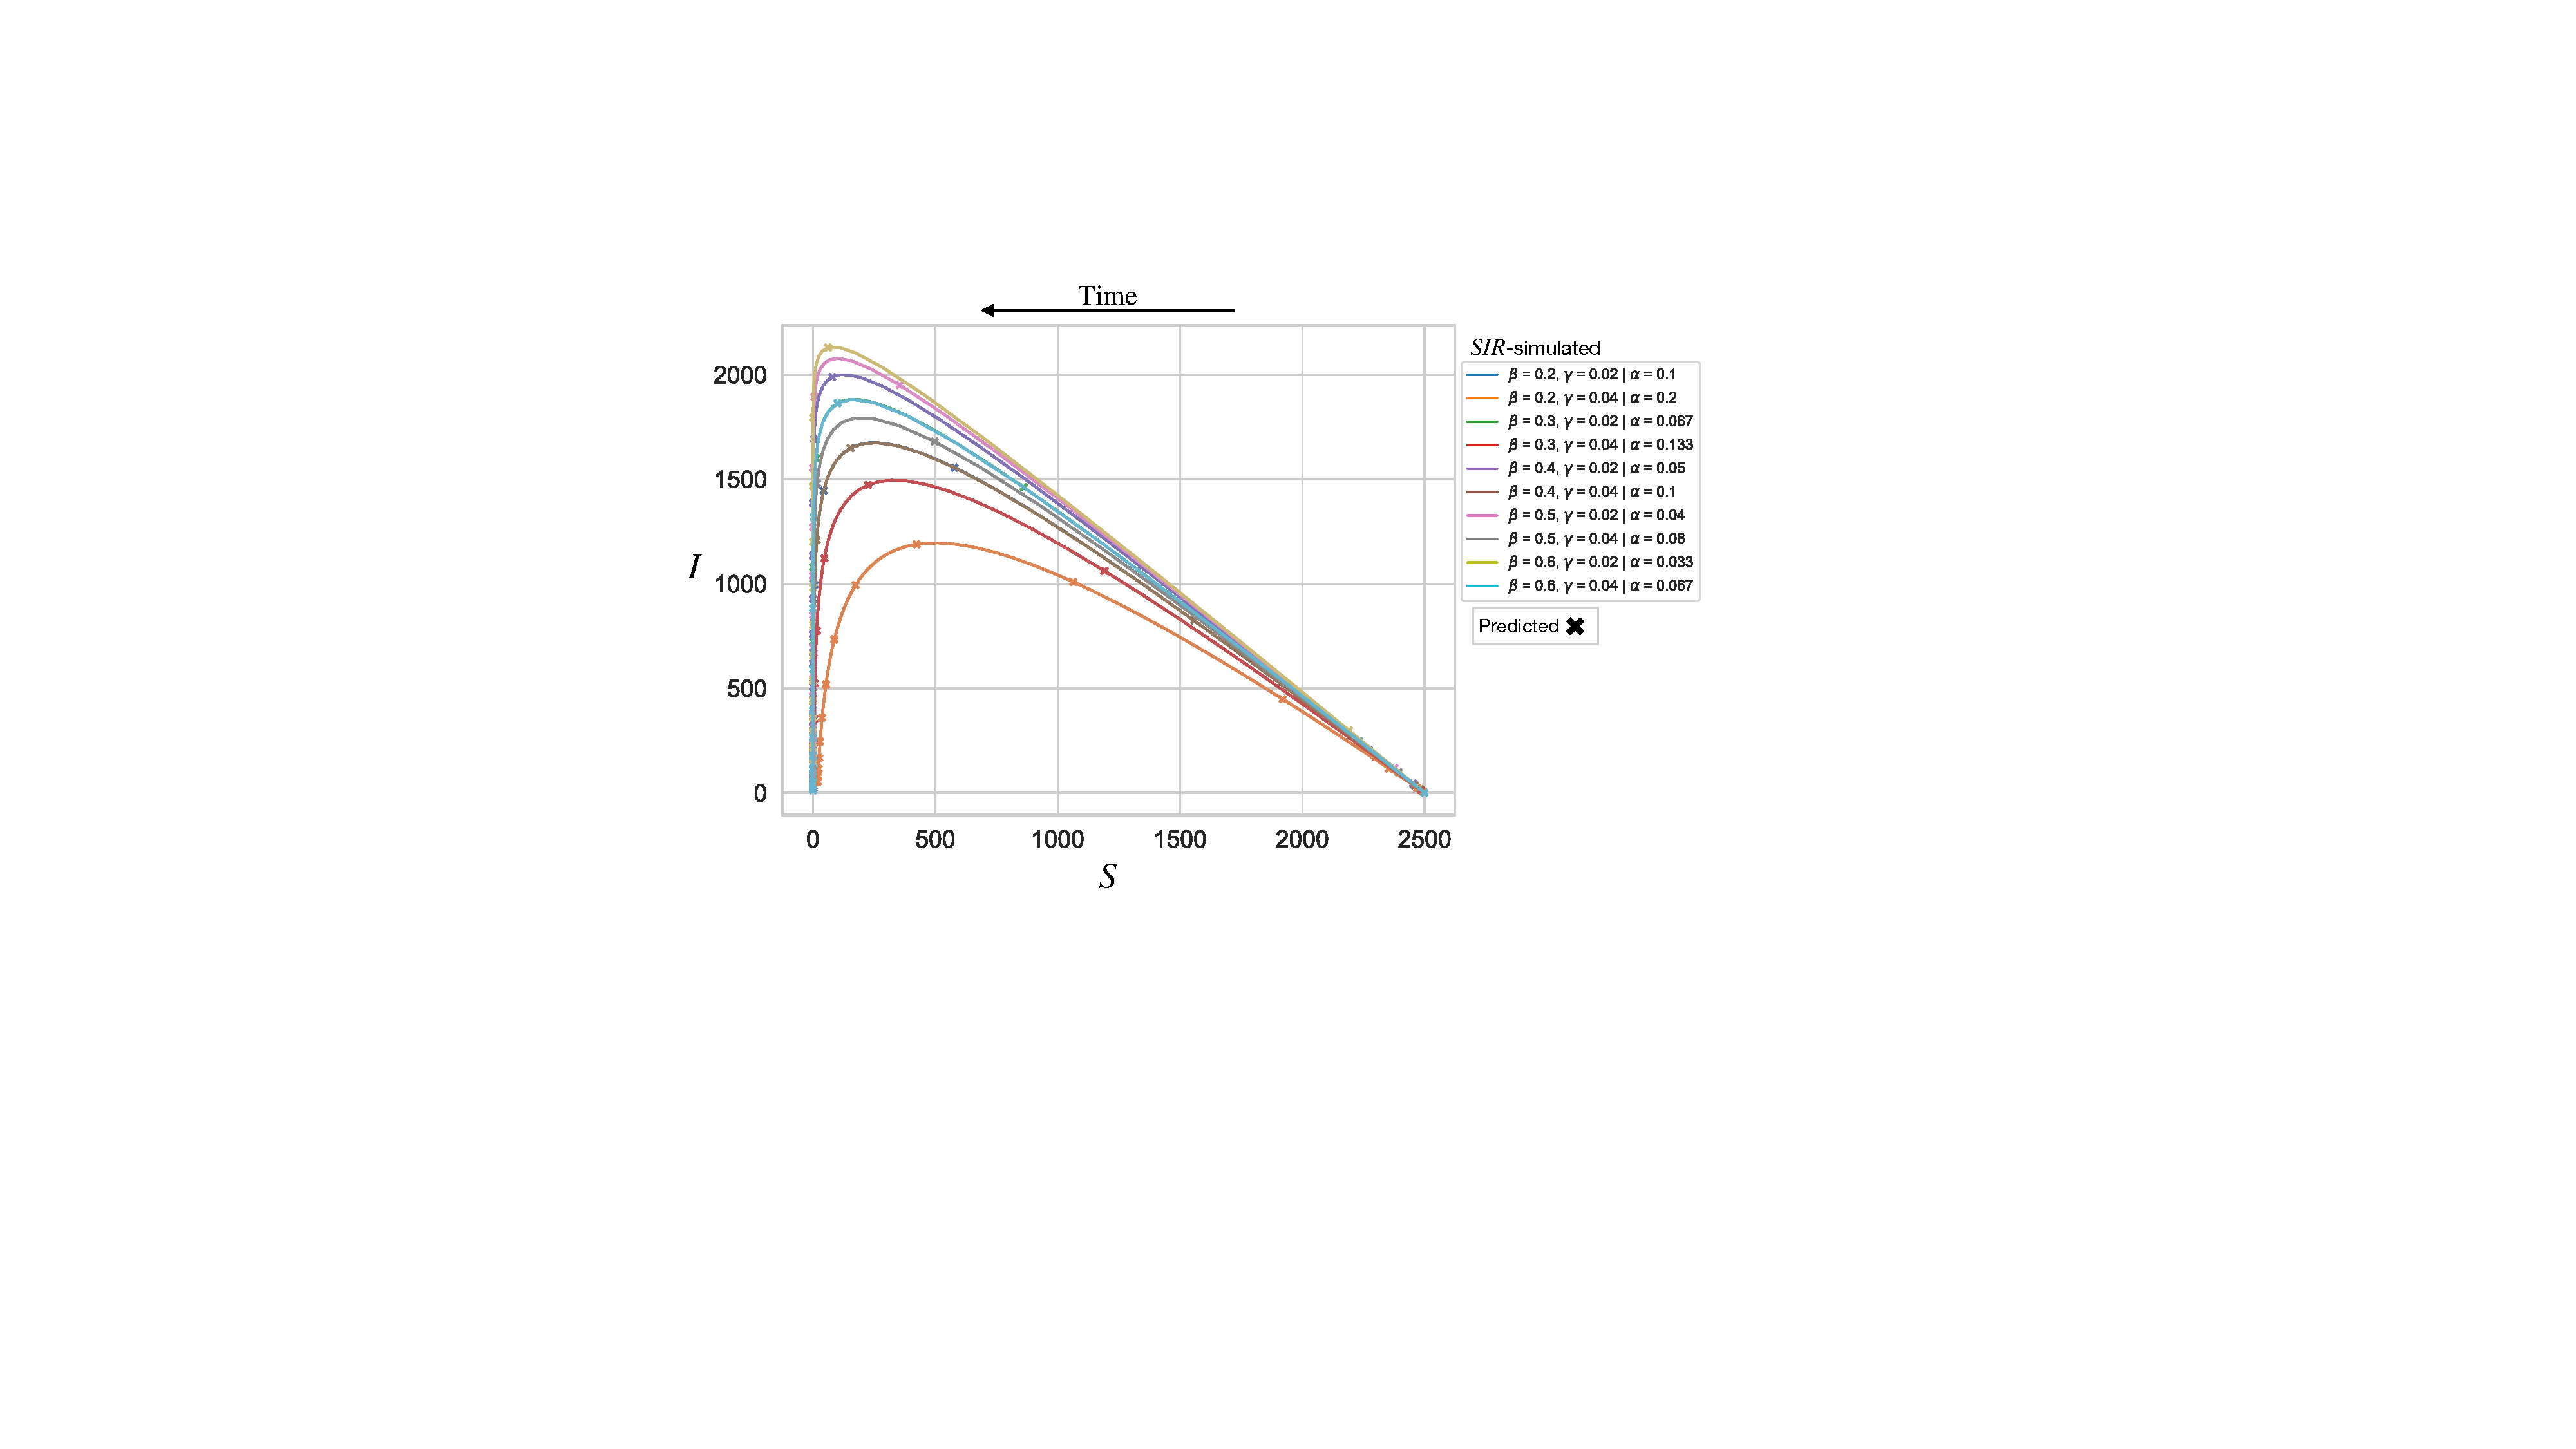
\includegraphics[scale=0.54]{chapter5/figures/fig2-sir-fitting-A.pdf}
    \caption{Infected hosts are plotted as a function hosts, according to the $SIR$ model for various ratios of $\alpha=\gamma / \beta$.
            Initial conditions began from one infected and 2500 susceptible hosts\textemdash equivalent to a $500\times500$ domain at tree density $0.01$.
            Numerical solutions of the $SIR$ model are plotted against predictions from equation \ref{eq:SIR-1param1}, shown as crosses.}
    \label{fig:sir-fitting-a}
\end{figure}

The standard $SIR$ model has no well-known analytic solution, which complicates model fitting.
As such, a simplified scheme that reduced the $SIR$ model to one parameter was used as a comparative tool to access NLM simulations.
Previously in chapter \ref{ch:dispersal-model}, details were omitted about the behaviour of equation \ref{eq:SIR-1param1}, i.e.
\[
I(S) = -S +  N \Big( 1 + \alpha \ln(S / S_0) \Big)
\]
In Figure \ref{fig:sir-fitting-a}, numerical simulations of the $SIR$ model are compared against analytic predictions from equation \ref{eq:SIR-1param1}.
Specifically, the $SIR$ model was simulated\textemdash using the Euler method\textemdash for various combinations of infectivity rate $\beta$ and removal rate $\gamma$ beginning from
one initially infected and 2500 susceptible hosts.
Numerical $SIR$ simulations and predictions of infected hosts $I$ (from equation \ref{eq:SIR-1param1}) are shown as solid lines and crosses respectively.
As the ratio $\alpha=\gamma/\beta$ decreases, a sharper rise in the infections field $I$ results, indicating a more infectious outbreak.
In contrast, a larger value of $\alpha$ defines a smoother curve which attains a lower peak.
Although equation \ref{eq:SIR-1param1} has clear limitations and descriptive power, it allows a simple one-parameter model to fit the NLM against.

\newpage

\section{Exponentially distributed times}

\begin{figure}[h]
    \centering
    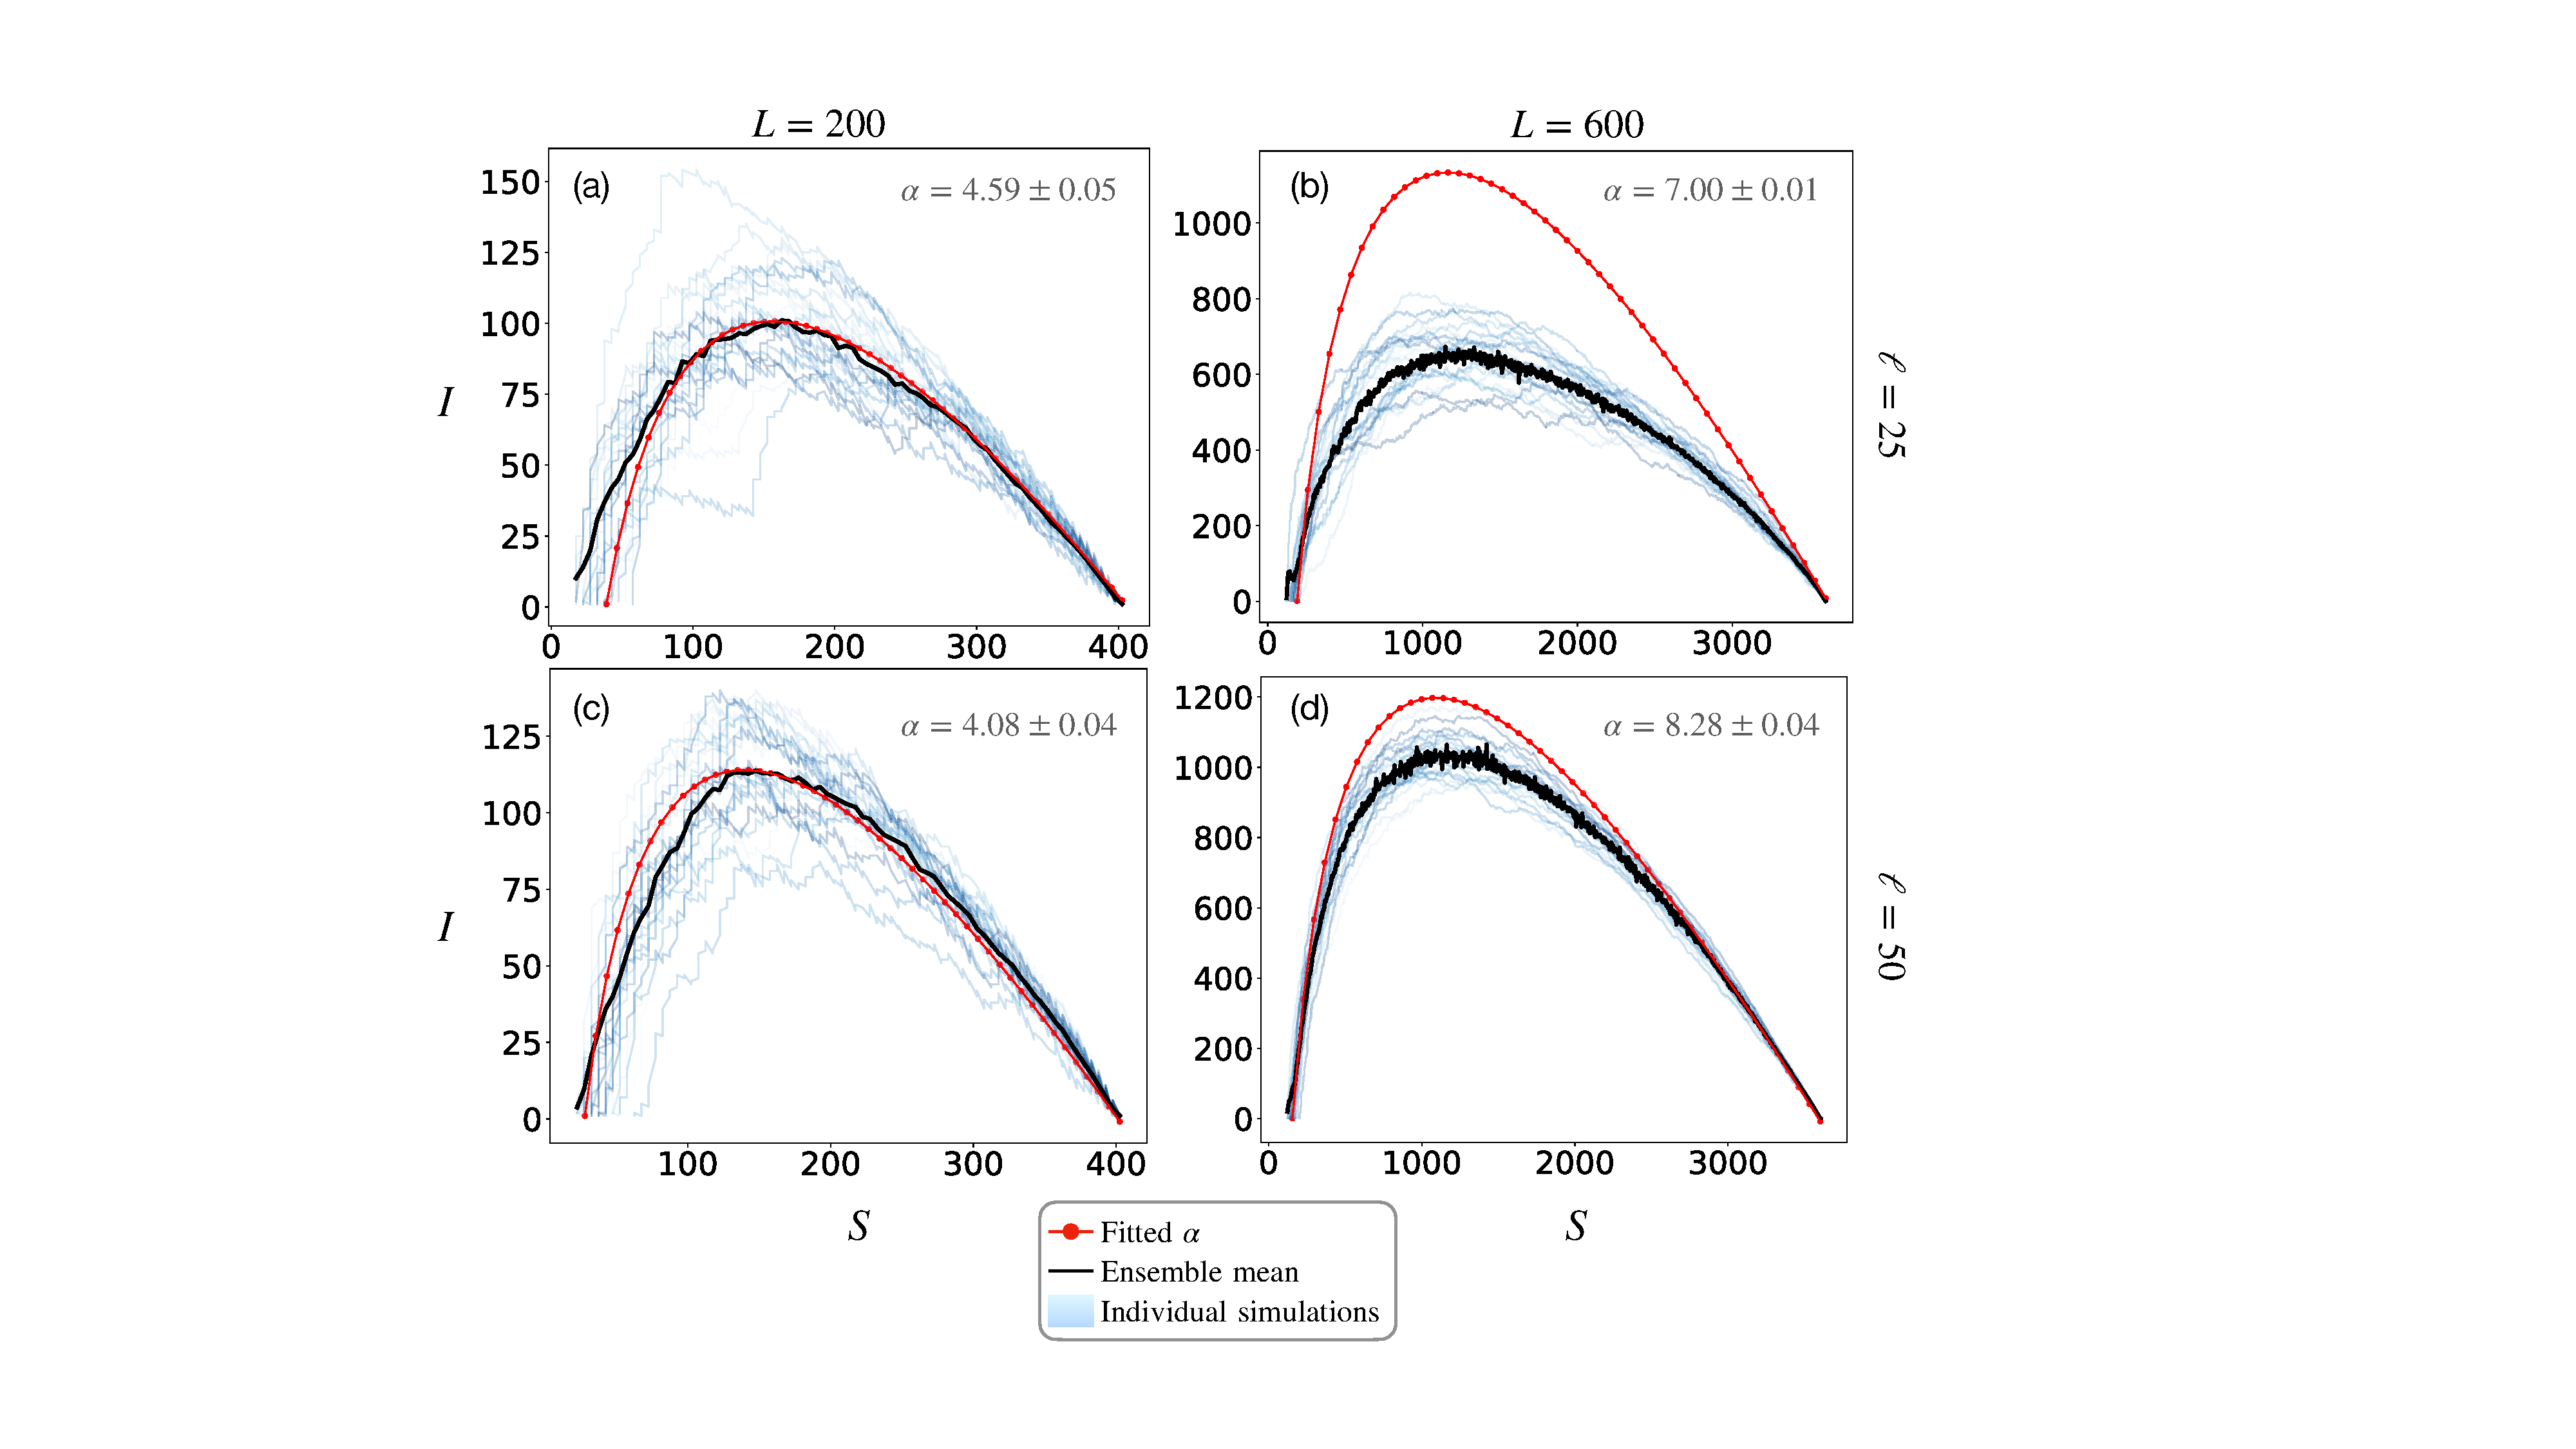
\includegraphics[scale=0.4]{chapter5/figures/fig2-sir-fitting-exp.pdf}
    \caption{Caption}
    \label{fig:SIR-fitting-expontial}
\end{figure}


\label{a:exponentially-distributed-lt}
In chapter 5 the NLM was constructed with uniform transitions into the removed compartment. 
Here, uniform refers to a transition into the $R$ compartment exactly $T$ time-steps after the host becomes infected.
Arguably, uniform life-time transitions are simple and unrealistic.
As such, the NLM constructed in chapter \ref{ch:dispersal-model} was re-run with exponentially-distributed life-times. 
Figure \ref{fig:SIR-fitting-expontial} shows the SIR fitting procedure against the exponentially-distributed variant of the NLM. 
Model behaviour in Figure \ref{fig:SIR-fitting-expontial} looks much the same, although fitting the exponentially-distributed NLM to the SIR model resulted in a closer fit for all panels except (b). 
Figure \ref{fig:SIR-fitting-expontial}(b) shows a much larger disparity between the NLM and SIR model.


\newpage

\section{Combining probabilities in the NLM}
\label{A:combiniing-probabilities}

As mentioned in section \ref{sec:contract-traced-R0}, probabilities in the NLM are simplistic.
That is, we consider interactions between infected and susceptible hosts one by one at each time-step.
In pseudo-code, the essential implementation follows:

\begin{lstlisting}[style=pythoncode,
    caption = ,
    label = py:rand]

def run_algorithm():
    for time_step in range(run_times):  # iterate over time
        for infected_tree in I_arr:  # iterate over I trees
            for susceptible_tree in S_arr:  # iterate over S trees
                Pr(S_x --> I_x ; I_y)
                ...
                ...
                ...
\end{lstlisting}

although these singular between-tree interactions (handled sequentially) are sufficient to model the spread of disease, it would be interesting to compare against a `multi-interaction' implementation by combining probabilities of the form:
\begin{equation}
    Pr(S_x \rightarrow I_{x}; I_{y1}, I_{y2})
\end{equation}
where $I_{y1}$ and $I_{y2}$ are two distinct trees and $y1 \neq y2$.
Now, suppose infection pressure from the two infected trees at location $y1$ and $y2$ simultaneously interact with one susceptible tree at location $x$.
Over a single time-step the combined probability is then:
\begin{equation}
    Pr(S_x \rightarrow I_{x}; I_{y1}, I_{y2}) = P_{y1} + P_{y2} - \big[ P_{y1} \cap P_{yn} \big] 
\end{equation}
where $P_{y1}$ and $P_{y2}$ are the individual probabilities of transition due to $y1$ and $y2$ respectively.
Now, suppose there are $yN$ infected trees, the combined probability is given by the inclusion-exclusion principle:
\begin{equation}
\label{eq:combined-pr}
     Pr(S_x \rightarrow I_{x}; I_{y1}, I_{y2}...I_{yN}) = \sum_{k=1}^{N} \big(  -1 \big)^{k+1} \Big[ \sum _{1\leq y1 \leq y2 \leq....\leq P_{yk} \leq N} \big| P_{y1}\cap ...\cap P_{yk}  \big|   \Big]
\end{equation}

where each union $P_{y1} \cap ... \cap P_{yk}$ adds a small order correction to the original NLM formulation.
It must be remarked how equation \ref{eq:combined-pr} would incur a significant computational cost.
Moreover, because secondary can be induced under the influence of multiple sources the definition of $R_0$ becomes obscure.  
Although implementing equation \ref{eq:combined-pr} would be an interesting\textemdash and potentially insightful\textemdash endeavour, the analysis was not undertaken.

\section{Contact-tracing $R_0$}
\label{A:R0-contact-traced-mortality}

\begin{figure}
    \centering
    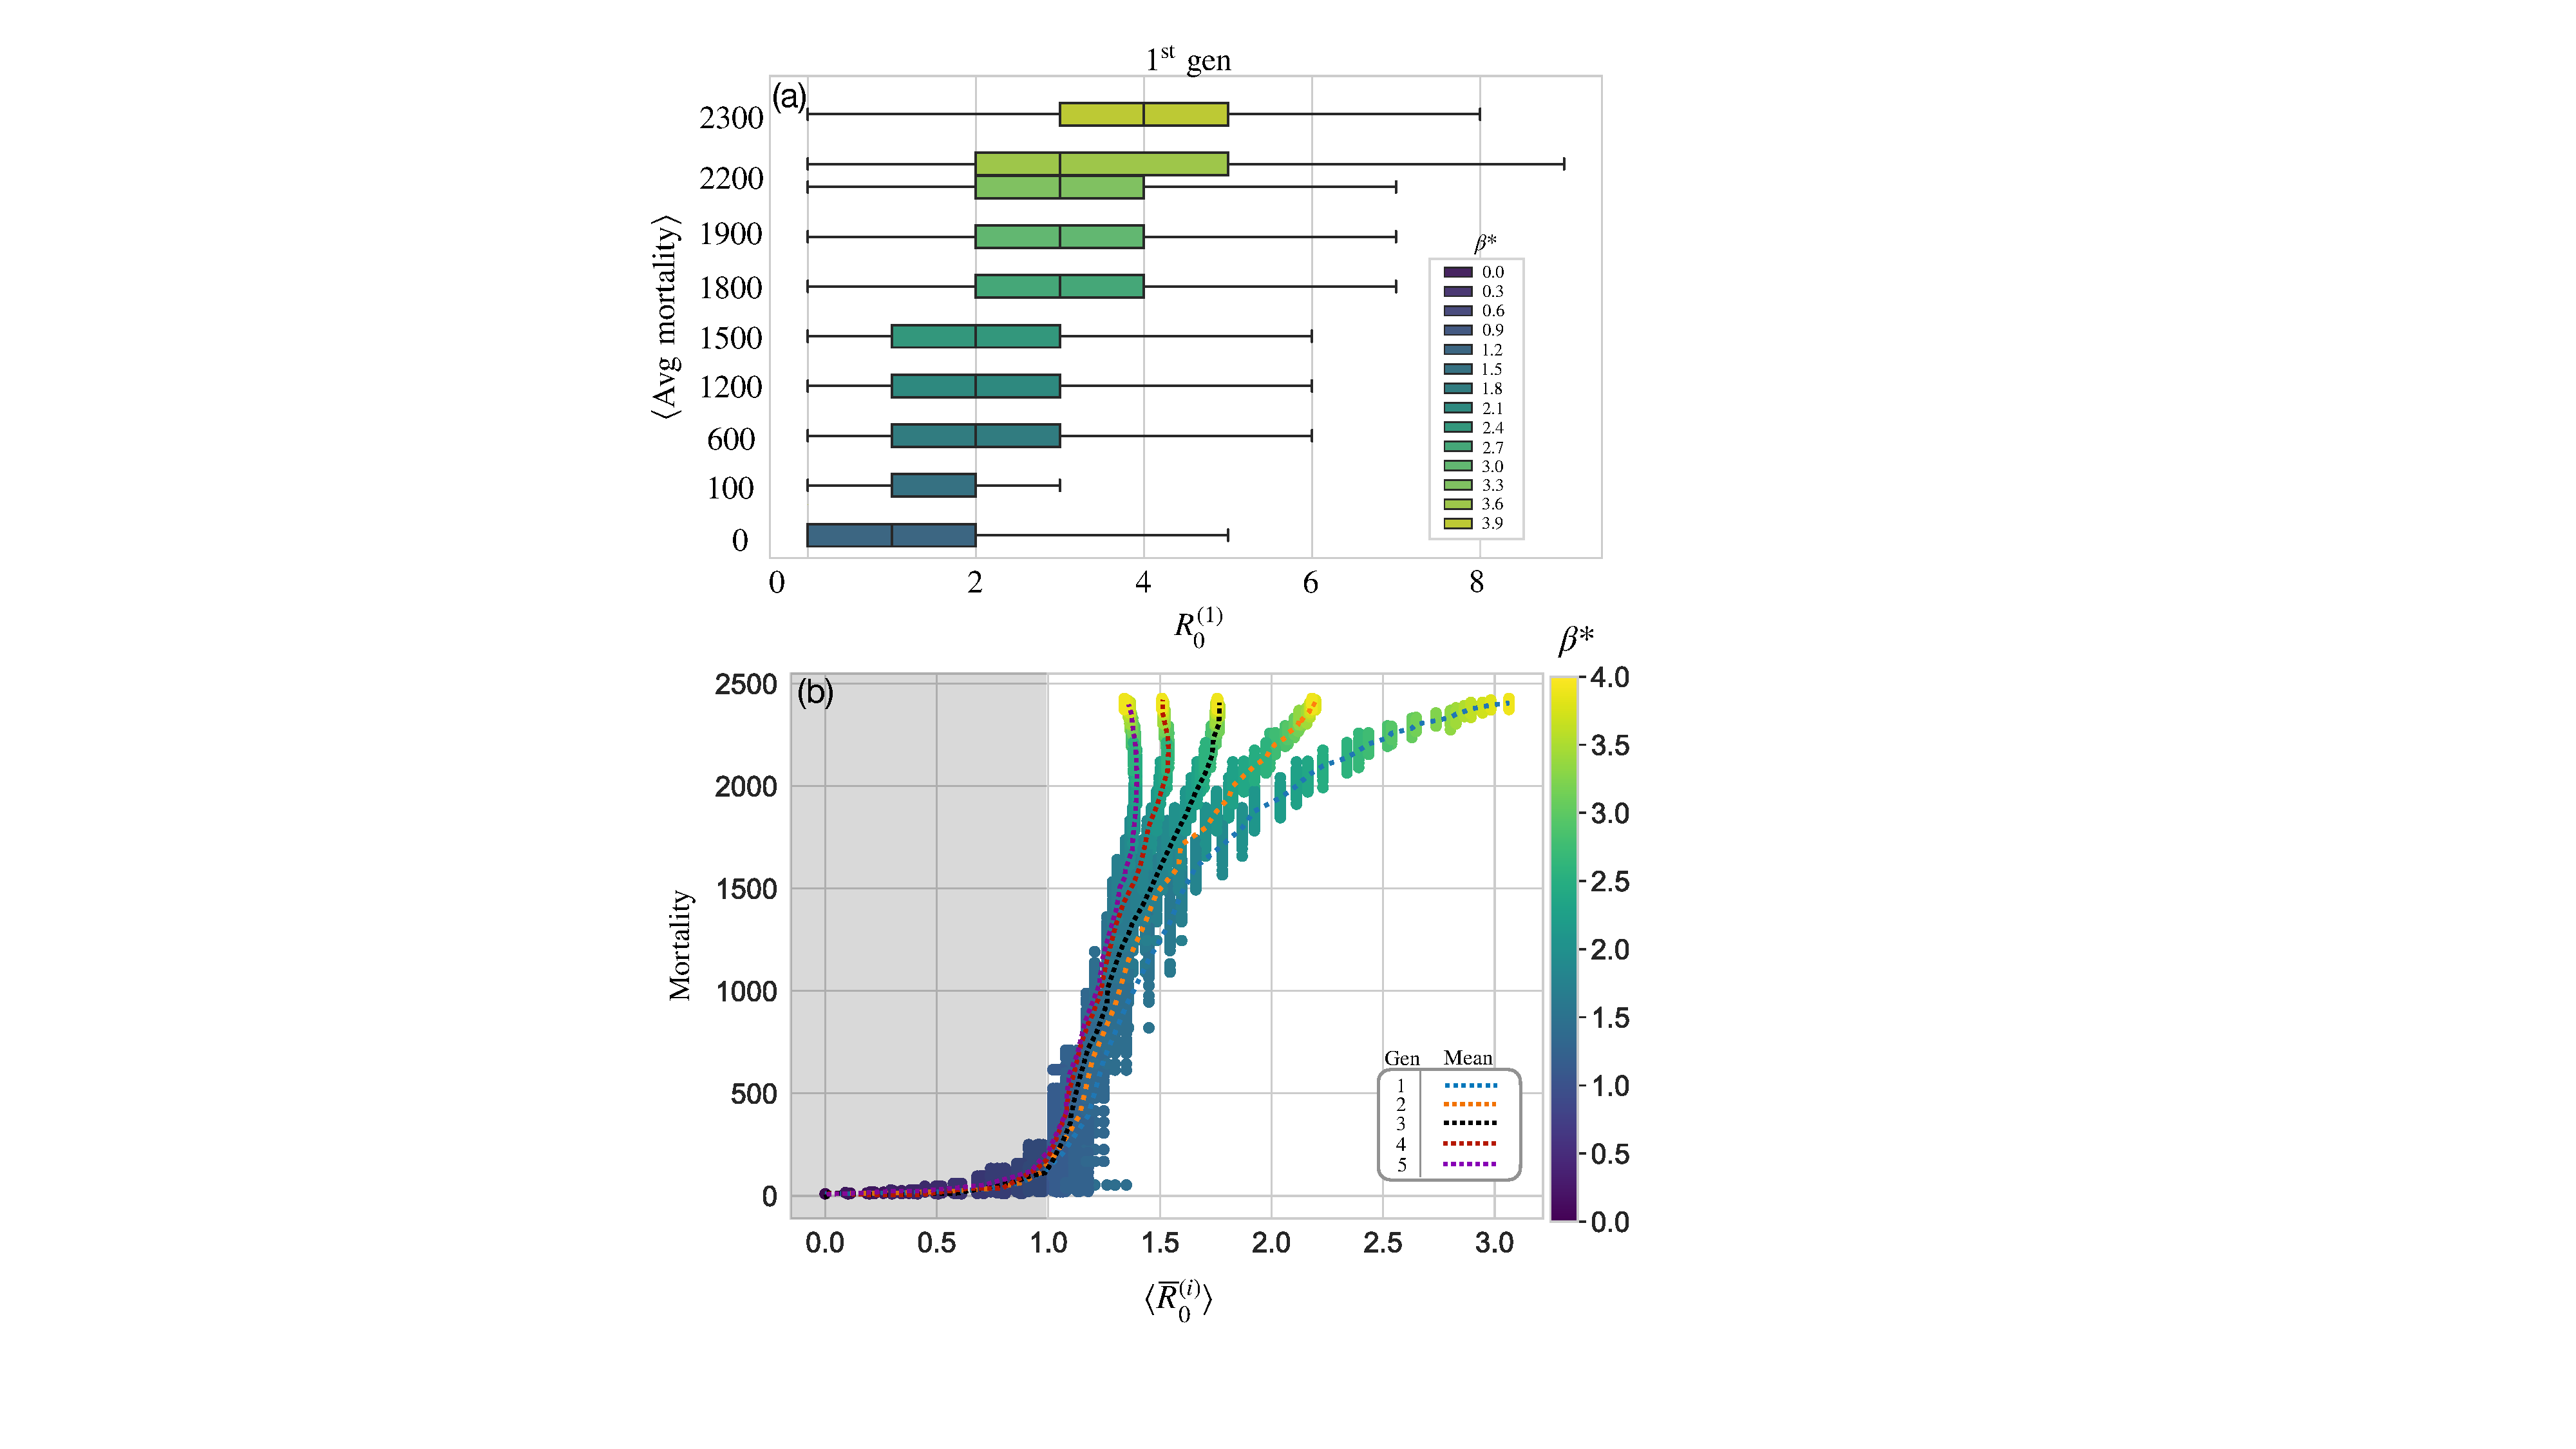
\includegraphics[scale=0.60]{chapter5/figures/fig6-R0-contact-vs-mortality-A.pdf}
    \caption{Comparing the contact-traced reproduction ratio against tree mortality. (a) Inverting the plot of Figure \ref{fig:contact-trace-vs-mortality} to show the spread of $R_0^{(1)}$ against the ensemble averaged tree mortality. (b)
    Re-running the ensemble shown in Figure \ref{fig:contact-trace-vs-mortality} with $10$ initially infected trees. The threshold appears more abrupt and stochasticity is reduced.}
    \label{fig:R0-contact-vs-morality-A}
\end{figure}

In Figure \ref{fig:R0-contact-vs-morality-A}(a), we invert the plot (shown in chapter \ref{ch:dispersal-model} Figure \ref{fig:contact-trace-vs-mortality}) and show the range of first generation reproduction ratios $R_0^{(i1)}$ against the ensemble-averaged tree mortality.
Inverting the plot gives information about the spread of $R_0^{(1)}$;
as we can see, low values of infectiviy produce a skewed distribution which becomes more centered as infectivity increases.
A threshold can be seen around $R_0^{(1)}=1$, although a number of simulations can produce a low-valued $R_0^{(1)}$ for any value of infectivity due to initial extinction events.

In chapter \ref{ch:dispersal-model} both the contact and analytic values of $R_0$ were computed/observed for a single infectious tree at the domain center.
As elaborated in chapter \ref{ch:dispersal-model}, initial stochastic forces had the tendency to reduce the chance of epidemic by causing early extinction events\textemdash thereby reducing the mean tree mortality.
However, a number of initial conditions are possible.
As such, the plot of Figure \ref{fig:contact-trace-vs-mortality} was re-run with $10$ infectious trees in the domain center at $t=0$ to test how initial stochasticity in the system changes, shown by Figure \ref{fig:R0-contact-vs-morality-A}(b).

As expected, increasing the number of infected trees at $t=0$ reduces stochastic and early extinction events;
this is demonstrated by noting that Figure \ref{fig:R0-contact-vs-morality-A}(b) has a smoother ensemble mean, and no instances of zero mortality for highly infectious epidemics (c.f. the bottom right hand side of Figure \ref{fig:contact-trace-vs-mortality} where multiple observations can be seen of zero tree mortality for high $\beta^*$).
Surprisingly, for later generations the degree of inflexion for $R_0^{(4)}$-$R_0^{(5)}$ is reduced at high $\beta^*$ in comparison to Figure \ref{fig:contact-trace-vs-mortality},

\newpage


\chapter{Seasonal $SEIR$ model of Ash dieback}

\label{section:ga-SEIR-variant}
\begin{itemize}
    \item The Gaussian and inverse power-law models are distinct and could be considered to have different infecitivity parameters $\beta_{ga}$ and $\beta_{pl}$k.
\end{itemize}

\section{Connected component analysis}

\blindtext

\blindtext


\chapter{Towards landscape-level control}

\blindtext

\blindtext

\begin{figure}
    \centering
    \includegraphics[scale=0.5]{appendix/Graphical_Abstract.pdf}
    \caption{Caption}
    \label{fig:my_label}
\end{figure}






% -----------------------------------------------------------------------------
% Reference list
% \bibliographystyle{apalike}. 
\bibliographystyle{acm}
\bibliography{references}
\end{document}
